\documentclass[twoside]{book}

% Packages required by doxygen
\usepackage{fixltx2e}
\usepackage{calc}
\usepackage{doxygen}
\usepackage[export]{adjustbox} % also loads graphicx
\usepackage{graphicx}
\usepackage[utf8]{inputenc}
\usepackage{makeidx}
\usepackage{multicol}
\usepackage{multirow}
\PassOptionsToPackage{warn}{textcomp}
\usepackage{textcomp}
\usepackage[nointegrals]{wasysym}
\usepackage[table]{xcolor}

% Font selection
\usepackage[T1]{fontenc}
\usepackage[scaled=.90]{helvet}
\usepackage{courier}
\usepackage{amssymb}
\usepackage{sectsty}
\renewcommand{\familydefault}{\sfdefault}
\allsectionsfont{%
  \fontseries{bc}\selectfont%
  \color{darkgray}%
}
\renewcommand{\DoxyLabelFont}{%
  \fontseries{bc}\selectfont%
  \color{darkgray}%
}
\newcommand{\+}{\discretionary{\mbox{\scriptsize$\hookleftarrow$}}{}{}}

% Page & text layout
\usepackage{geometry}
\geometry{%
  a4paper,%
  top=2.5cm,%
  bottom=2.5cm,%
  left=2.5cm,%
  right=2.5cm%
}
\tolerance=750
\hfuzz=15pt
\hbadness=750
\setlength{\emergencystretch}{15pt}
\setlength{\parindent}{0cm}
\setlength{\parskip}{3ex plus 2ex minus 2ex}
\makeatletter
\renewcommand{\paragraph}{%
  \@startsection{paragraph}{4}{0ex}{-1.0ex}{1.0ex}{%
    \normalfont\normalsize\bfseries\SS@parafont%
  }%
}
\renewcommand{\subparagraph}{%
  \@startsection{subparagraph}{5}{0ex}{-1.0ex}{1.0ex}{%
    \normalfont\normalsize\bfseries\SS@subparafont%
  }%
}
\makeatother

% Headers & footers
\usepackage{fancyhdr}
\pagestyle{fancyplain}
\fancyhead[LE]{\fancyplain{}{\bfseries\thepage}}
\fancyhead[CE]{\fancyplain{}{}}
\fancyhead[RE]{\fancyplain{}{\bfseries\leftmark}}
\fancyhead[LO]{\fancyplain{}{\bfseries\rightmark}}
\fancyhead[CO]{\fancyplain{}{}}
\fancyhead[RO]{\fancyplain{}{\bfseries\thepage}}
\fancyfoot[LE]{\fancyplain{}{}}
\fancyfoot[CE]{\fancyplain{}{}}
\fancyfoot[RE]{\fancyplain{}{\bfseries\scriptsize Generated by Doxygen }}
\fancyfoot[LO]{\fancyplain{}{\bfseries\scriptsize Generated by Doxygen }}
\fancyfoot[CO]{\fancyplain{}{}}
\fancyfoot[RO]{\fancyplain{}{}}
\renewcommand{\footrulewidth}{0.4pt}
\renewcommand{\chaptermark}[1]{%
  \markboth{#1}{}%
}
\renewcommand{\sectionmark}[1]{%
  \markright{\thesection\ #1}%
}

% Indices & bibliography
\usepackage{natbib}
\usepackage[titles]{tocloft}
\setcounter{tocdepth}{3}
\setcounter{secnumdepth}{5}
\makeindex

% Hyperlinks (required, but should be loaded last)
\usepackage{ifpdf}
\ifpdf
  \usepackage[pdftex,pagebackref=true]{hyperref}
\else
  \usepackage[ps2pdf,pagebackref=true]{hyperref}
\fi
\hypersetup{%
  colorlinks=true,%
  linkcolor=blue,%
  citecolor=blue,%
  unicode%
}

% Custom commands
\newcommand{\clearemptydoublepage}{%
  \newpage{\pagestyle{empty}\cleardoublepage}%
}

\usepackage{caption}
\captionsetup{labelsep=space,justification=centering,font={bf},singlelinecheck=off,skip=4pt,position=top}

%===== C O N T E N T S =====

\begin{document}

% Titlepage & ToC
\hypersetup{pageanchor=false,
             bookmarksnumbered=true,
             pdfencoding=unicode
            }
\pagenumbering{alph}
\begin{titlepage}
\vspace*{7cm}
\begin{center}%
{\Large My Project }\\
\vspace*{1cm}
{\large Generated by Doxygen 1.8.12}\\
\end{center}
\end{titlepage}
\clearemptydoublepage
\pagenumbering{roman}
\tableofcontents
\clearemptydoublepage
\pagenumbering{arabic}
\hypersetup{pageanchor=true}

%--- Begin generated contents ---
\chapter{Namespace Index}
\section{Namespace List}
Here is a list of all documented namespaces with brief descriptions\+:\begin{DoxyCompactList}
\item\contentsline{section}{\hyperlink{namespace_blaze___brigade}{Blaze\+\_\+\+Brigade} }{\pageref{namespace_blaze___brigade}}{}
\item\contentsline{section}{\hyperlink{namespace_controller}{Controller} \\*The controller in M\+VC. These classes will control how the \hyperlink{namespace_model}{Model} is used, and how the \hyperlink{namespace_view}{View} will be displayed to the user. }{\pageref{namespace_controller}}{}
\item\contentsline{section}{\hyperlink{namespace_model}{Model} \\*The model in M\+VC. These classes contain the structure of the game, and will be controlled by \hyperlink{namespace_controller}{Controller}, and displayed in \hyperlink{namespace_view}{View}. }{\pageref{namespace_model}}{}
\item\contentsline{section}{\hyperlink{namespace_model_1_1_map_module}{Model.\+Map\+Module} \\*The Map Module, containing all classes related to setting up the working game map. }{\pageref{namespace_model_1_1_map_module}}{}
\item\contentsline{section}{\hyperlink{namespace_model_1_1_unit_module}{Model.\+Unit\+Module} \\*The module containing all unit related classes and interface. }{\pageref{namespace_model_1_1_unit_module}}{}
\item\contentsline{section}{\hyperlink{namespace_model_1_1_weapon_module}{Model.\+Weapon\+Module} \\*The module containing all weapon related classes and interfaces. }{\pageref{namespace_model_1_1_weapon_module}}{}
\item\contentsline{section}{\hyperlink{namespace_view}{View} \\*The view in M\+VC. These classes deal with the view that the user sees in the game. }{\pageref{namespace_view}}{}
\item\contentsline{section}{\hyperlink{namespace_view_1_1_menu_module}{View.\+Menu\+Module} \\*The Menu Module containing all menu related classes. }{\pageref{namespace_view_1_1_menu_module}}{}
\end{DoxyCompactList}

\chapter{Hierarchical Index}
\section{Class Hierarchy}
This inheritance list is sorted roughly, but not completely, alphabetically\+:\begin{DoxyCompactList}
\item \contentsline{section}{View.\+Animation}{\pageref{class_view_1_1_animation}}{}
\item \contentsline{section}{Model.\+Button}{\pageref{class_model_1_1_button}}{}
\item \contentsline{section}{View.\+Camera}{\pageref{class_view_1_1_camera}}{}
\item \contentsline{section}{Controller.\+Damage\+Calculations}{\pageref{class_controller_1_1_damage_calculations}}{}
\item \contentsline{section}{View.\+Draw\+Class}{\pageref{class_view_1_1_draw_class}}{}
\item Form\begin{DoxyCompactList}
\item \contentsline{section}{View.\+Menu\+Module.\+How\+To\+Play}{\pageref{class_view_1_1_menu_module_1_1_how_to_play}}{}
\item \contentsline{section}{View.\+Menu\+Module.\+How\+To\+Play2}{\pageref{class_view_1_1_menu_module_1_1_how_to_play2}}{}
\item \contentsline{section}{View.\+Menu\+Module.\+How\+To\+Play3}{\pageref{class_view_1_1_menu_module_1_1_how_to_play3}}{}
\item \contentsline{section}{View.\+Menu\+Module.\+Main\+Menu}{\pageref{class_view_1_1_menu_module_1_1_main_menu}}{}
\end{DoxyCompactList}
\item Game\begin{DoxyCompactList}
\item \contentsline{section}{Controller.\+Game}{\pageref{class_controller_1_1_game}}{}
\end{DoxyCompactList}
\item \contentsline{section}{Controller.\+Game\+Function}{\pageref{class_controller_1_1_game_function}}{}
\item \contentsline{section}{Model.\+Game\+State}{\pageref{class_model_1_1_game_state}}{}
\item \contentsline{section}{Model.\+Map\+Module.\+Graph}{\pageref{class_model_1_1_map_module_1_1_graph}}{}
\item \contentsline{section}{Controller.\+Mouse\+Handler}{\pageref{class_controller_1_1_mouse_handler}}{}
\item \contentsline{section}{Model.\+Map\+Module.\+Node}{\pageref{class_model_1_1_map_module_1_1_node}}{}
\item \contentsline{section}{Model.\+Player}{\pageref{class_model_1_1_player}}{}
\item \contentsline{section}{View.\+Sounds}{\pageref{class_view_1_1_sounds}}{}
\item \contentsline{section}{Model.\+Unit\+Module.\+Unit}{\pageref{interface_model_1_1_unit_module_1_1_unit}}{}
\begin{DoxyCompactList}
\item \contentsline{section}{Model.\+Unit\+Module.\+Archer}{\pageref{class_model_1_1_unit_module_1_1_archer}}{}
\item \contentsline{section}{Model.\+Unit\+Module.\+Mage}{\pageref{class_model_1_1_unit_module_1_1_mage}}{}
\item \contentsline{section}{Model.\+Unit\+Module.\+Warrior}{\pageref{class_model_1_1_unit_module_1_1_warrior}}{}
\end{DoxyCompactList}
\item \contentsline{section}{Model.\+Weapon\+Module.\+Weapon}{\pageref{interface_model_1_1_weapon_module_1_1_weapon}}{}
\begin{DoxyCompactList}
\item \contentsline{section}{Model.\+Weapon\+Module.\+Bronze\+Sword}{\pageref{class_model_1_1_weapon_module_1_1_bronze_sword}}{}
\item \contentsline{section}{Model.\+Weapon\+Module.\+Fireball}{\pageref{class_model_1_1_weapon_module_1_1_fireball}}{}
\item \contentsline{section}{Model.\+Weapon\+Module.\+Fireblast}{\pageref{class_model_1_1_weapon_module_1_1_fireblast}}{}
\item \contentsline{section}{Model.\+Weapon\+Module.\+Iron\+Sword}{\pageref{class_model_1_1_weapon_module_1_1_iron_sword}}{}
\item \contentsline{section}{Model.\+Weapon\+Module.\+Long\+Bow}{\pageref{class_model_1_1_weapon_module_1_1_long_bow}}{}
\item \contentsline{section}{Model.\+Weapon\+Module.\+Short\+Bow}{\pageref{class_model_1_1_weapon_module_1_1_short_bow}}{}
\end{DoxyCompactList}
\end{DoxyCompactList}

\chapter{Class Index}
\section{Class List}
Here are the classes, structs, unions and interfaces with brief descriptions\+:\begin{DoxyCompactList}
\item\contentsline{section}{\hyperlink{class_view_1_1_animation}{View.\+Animation} \\*Static class containing all animation methods }{\pageref{class_view_1_1_animation}}{}
\item\contentsline{section}{\hyperlink{class_model_1_1_unit_module_1_1_archer}{Model.\+Unit\+Module.\+Archer} \\*The \hyperlink{class_model_1_1_unit_module_1_1_archer}{Archer} model class, extends \hyperlink{interface_model_1_1_unit_module_1_1_unit}{Unit}. This unit has a high skill and speed, and excels in dealing accurate ranged, high critical, physical attacks, but suffers from overall defense against physical attacks. }{\pageref{class_model_1_1_unit_module_1_1_archer}}{}
\item\contentsline{section}{\hyperlink{class_model_1_1_weapon_module_1_1_bronze_sword}{Model.\+Weapon\+Module.\+Bronze\+Sword} \\*Melee Physical \hyperlink{interface_model_1_1_weapon_module_1_1_weapon}{Weapon}. }{\pageref{class_model_1_1_weapon_module_1_1_bronze_sword}}{}
\item\contentsline{section}{\hyperlink{class_model_1_1_button}{Model.\+Button} \\*Buttons for the drop down menu buttons when selecting units. }{\pageref{class_model_1_1_button}}{}
\item\contentsline{section}{\hyperlink{class_view_1_1_camera}{View.\+Camera} \\*The camera class for making the scrollable camera. }{\pageref{class_view_1_1_camera}}{}
\item\contentsline{section}{\hyperlink{class_controller_1_1_damage_calculations}{Controller.\+Damage\+Calculations} \\*This class calculates all damage related calculations }{\pageref{class_controller_1_1_damage_calculations}}{}
\item\contentsline{section}{\hyperlink{class_view_1_1_draw_class}{View.\+Draw\+Class} \\*Draw Class containing all the different draw methods }{\pageref{class_view_1_1_draw_class}}{}
\item\contentsline{section}{\hyperlink{class_model_1_1_weapon_module_1_1_fireball}{Model.\+Weapon\+Module.\+Fireball} \\*Ranged Magical \hyperlink{interface_model_1_1_weapon_module_1_1_weapon}{Weapon}. }{\pageref{class_model_1_1_weapon_module_1_1_fireball}}{}
\item\contentsline{section}{\hyperlink{class_model_1_1_weapon_module_1_1_fireblast}{Model.\+Weapon\+Module.\+Fireblast} \\*Ranged Magical \hyperlink{interface_model_1_1_weapon_module_1_1_weapon}{Weapon}. }{\pageref{class_model_1_1_weapon_module_1_1_fireblast}}{}
\item\contentsline{section}{\hyperlink{class_controller_1_1_game}{Controller.\+Game} \\*Main \hyperlink{namespace_controller}{Controller} for game }{\pageref{class_controller_1_1_game}}{}
\item\contentsline{section}{\hyperlink{class_controller_1_1_game_function}{Controller.\+Game\+Function} \\*Contains functions that update the \hyperlink{namespace_model}{Model}. }{\pageref{class_controller_1_1_game_function}}{}
\item\contentsline{section}{\hyperlink{class_model_1_1_game_state}{Model.\+Game\+State} \\*This class holds states in the scope of the entire gameplay. }{\pageref{class_model_1_1_game_state}}{}
\item\contentsline{section}{\hyperlink{class_model_1_1_map_module_1_1_graph}{Model.\+Map\+Module.\+Graph} \\*Structure that represents the game map. }{\pageref{class_model_1_1_map_module_1_1_graph}}{}
\item\contentsline{section}{\hyperlink{class_view_1_1_menu_module_1_1_how_to_play}{View.\+Menu\+Module.\+How\+To\+Play} \\*How to Play Menu }{\pageref{class_view_1_1_menu_module_1_1_how_to_play}}{}
\item\contentsline{section}{\hyperlink{class_view_1_1_menu_module_1_1_how_to_play2}{View.\+Menu\+Module.\+How\+To\+Play2} \\*How to Play Menu 2 is opened with next is clicked on \hyperlink{class_view_1_1_menu_module_1_1_how_to_play}{How\+To\+Play} Menu }{\pageref{class_view_1_1_menu_module_1_1_how_to_play2}}{}
\item\contentsline{section}{\hyperlink{class_view_1_1_menu_module_1_1_how_to_play3}{View.\+Menu\+Module.\+How\+To\+Play3} \\*How to Play Menu 3 is opened with next is clicked on \hyperlink{class_view_1_1_menu_module_1_1_how_to_play2}{How\+To\+Play2} Menu }{\pageref{class_view_1_1_menu_module_1_1_how_to_play3}}{}
\item\contentsline{section}{\hyperlink{class_model_1_1_weapon_module_1_1_iron_sword}{Model.\+Weapon\+Module.\+Iron\+Sword} \\*Melee Physical \hyperlink{interface_model_1_1_weapon_module_1_1_weapon}{Weapon}. }{\pageref{class_model_1_1_weapon_module_1_1_iron_sword}}{}
\item\contentsline{section}{\hyperlink{class_model_1_1_weapon_module_1_1_long_bow}{Model.\+Weapon\+Module.\+Long\+Bow} \\*Ranged physical \hyperlink{interface_model_1_1_weapon_module_1_1_weapon}{Weapon}. }{\pageref{class_model_1_1_weapon_module_1_1_long_bow}}{}
\item\contentsline{section}{\hyperlink{class_model_1_1_unit_module_1_1_mage}{Model.\+Unit\+Module.\+Mage} \\*The \hyperlink{class_model_1_1_unit_module_1_1_mage}{Mage} model class, extends \hyperlink{interface_model_1_1_unit_module_1_1_unit}{Unit}. ~\newline
 This \hyperlink{interface_model_1_1_unit_module_1_1_unit}{Unit} has strong magical capabilities, and is capable of powerful ranged magic attacks, but makes up with poor physical stats. }{\pageref{class_model_1_1_unit_module_1_1_mage}}{}
\item\contentsline{section}{\hyperlink{class_view_1_1_menu_module_1_1_main_menu}{View.\+Menu\+Module.\+Main\+Menu} \\*The Main Menu class. This window is displayed upon starting game, and can link you to \hyperlink{class_view_1_1_menu_module_1_1_how_to_play}{How\+To\+Play} playing the Game. }{\pageref{class_view_1_1_menu_module_1_1_main_menu}}{}
\item\contentsline{section}{\hyperlink{class_controller_1_1_mouse_handler}{Controller.\+Mouse\+Handler} \\*Handles all user mouse input. }{\pageref{class_controller_1_1_mouse_handler}}{}
\item\contentsline{section}{\hyperlink{class_model_1_1_map_module_1_1_node}{Model.\+Map\+Module.\+Node} \\*Structure that represents a tile on the game map grid. }{\pageref{class_model_1_1_map_module_1_1_node}}{}
\item\contentsline{section}{\hyperlink{class_model_1_1_player}{Model.\+Player} \\*Represents a \hyperlink{class_model_1_1_player}{Player} in the game. }{\pageref{class_model_1_1_player}}{}
\item\contentsline{section}{\hyperlink{class_model_1_1_weapon_module_1_1_short_bow}{Model.\+Weapon\+Module.\+Short\+Bow} \\*Ranged physical \hyperlink{interface_model_1_1_weapon_module_1_1_weapon}{Weapon}. }{\pageref{class_model_1_1_weapon_module_1_1_short_bow}}{}
\item\contentsline{section}{\hyperlink{class_view_1_1_sounds}{View.\+Sounds} \\*Sound class containing methods to play all different sounds to be used in the game }{\pageref{class_view_1_1_sounds}}{}
\item\contentsline{section}{\hyperlink{interface_model_1_1_unit_module_1_1_unit}{Model.\+Unit\+Module.\+Unit} \\*\hyperlink{interface_model_1_1_unit_module_1_1_unit}{Unit} Interface for \hyperlink{class_model_1_1_unit_module_1_1_warrior}{Warrior}, \hyperlink{class_model_1_1_unit_module_1_1_mage}{Mage}, and \hyperlink{class_model_1_1_unit_module_1_1_archer}{Archer}. }{\pageref{interface_model_1_1_unit_module_1_1_unit}}{}
\item\contentsline{section}{\hyperlink{class_model_1_1_unit_module_1_1_warrior}{Model.\+Unit\+Module.\+Warrior} \\*The \hyperlink{class_model_1_1_unit_module_1_1_warrior}{Warrior} model class, extends \hyperlink{interface_model_1_1_unit_module_1_1_unit}{Unit}. This unit excels in dealing melee physical damage, with a high defense, but suffers from lack of any magical attack or resistance. }{\pageref{class_model_1_1_unit_module_1_1_warrior}}{}
\item\contentsline{section}{\hyperlink{interface_model_1_1_weapon_module_1_1_weapon}{Model.\+Weapon\+Module.\+Weapon} \\*\hyperlink{interface_model_1_1_weapon_module_1_1_weapon}{Weapon} Interface to be implemented when creating new weapons. }{\pageref{interface_model_1_1_weapon_module_1_1_weapon}}{}
\end{DoxyCompactList}

\chapter{Namespace Documentation}
\hypertarget{namespace_blaze___brigade}{}\section{Blaze\+\_\+\+Brigade Namespace Reference}
\label{namespace_blaze___brigade}\index{Blaze\+\_\+\+Brigade@{Blaze\+\_\+\+Brigade}}
\subsection*{Classes}
\begin{DoxyCompactItemize}
\item 
class {\bfseries Resource1}
\begin{DoxyCompactList}\small\item\em A strongly-\/typed resource class, for looking up localized strings, etc. \end{DoxyCompactList}\end{DoxyCompactItemize}

\hypertarget{namespace_controller}{}\section{Controller Namespace Reference}
\label{namespace_controller}\index{Controller@{Controller}}


The controller in M\+VC. These classes will control how the \hyperlink{namespace_model}{Model} is used, and how the \hyperlink{namespace_view}{View} will be displayed to the user.  


\subsection*{Classes}
\begin{DoxyCompactItemize}
\item 
class \hyperlink{class_controller_1_1_damage_calculations}{Damage\+Calculations}
\begin{DoxyCompactList}\small\item\em This class calculates all damage related calculations \end{DoxyCompactList}\item 
class \hyperlink{class_controller_1_1_game}{Game}
\begin{DoxyCompactList}\small\item\em Main \hyperlink{namespace_controller}{Controller} for game \end{DoxyCompactList}\item 
class \hyperlink{class_controller_1_1_game_function}{Game\+Function}
\begin{DoxyCompactList}\small\item\em Contains functions that update the \hyperlink{namespace_model}{Model}. \end{DoxyCompactList}\item 
class \hyperlink{class_controller_1_1_mouse_handler}{Mouse\+Handler}
\begin{DoxyCompactList}\small\item\em Handles all user mouse input. \end{DoxyCompactList}\end{DoxyCompactItemize}


\subsection{Detailed Description}
The controller in M\+VC. These classes will control how the \hyperlink{namespace_model}{Model} is used, and how the \hyperlink{namespace_view}{View} will be displayed to the user. 


\hypertarget{namespace_model}{}\section{Model Namespace Reference}
\label{namespace_model}\index{Model@{Model}}


The model in M\+VC. These classes contain the structure of the game, and will be controlled by \hyperlink{namespace_controller}{Controller}, and displayed in \hyperlink{namespace_view}{View}.  


\subsection*{Namespaces}
\begin{DoxyCompactItemize}
\item 
namespace \hyperlink{namespace_model_1_1_map_module}{Map\+Module}
\begin{DoxyCompactList}\small\item\em The Map Module, containing all classes related to setting up the working game map. \end{DoxyCompactList}\item 
namespace \hyperlink{namespace_model_1_1_unit_module}{Unit\+Module}
\begin{DoxyCompactList}\small\item\em The module containing all unit related classes and interface. \end{DoxyCompactList}\item 
namespace \hyperlink{namespace_model_1_1_weapon_module}{Weapon\+Module}
\begin{DoxyCompactList}\small\item\em The module containing all weapon related classes and interfaces. \end{DoxyCompactList}\end{DoxyCompactItemize}
\subsection*{Classes}
\begin{DoxyCompactItemize}
\item 
class \hyperlink{class_model_1_1_button}{Button}
\begin{DoxyCompactList}\small\item\em Buttons for the drop down menu buttons when selecting units. \end{DoxyCompactList}\item 
class \hyperlink{class_model_1_1_game_state}{Game\+State}
\begin{DoxyCompactList}\small\item\em This class holds states in the scope of the entire gameplay. \end{DoxyCompactList}\item 
class \hyperlink{class_model_1_1_player}{Player}
\begin{DoxyCompactList}\small\item\em Represents a \hyperlink{class_model_1_1_player}{Player} in the game. \end{DoxyCompactList}\end{DoxyCompactItemize}
\subsection*{Enumerations}
\begin{DoxyCompactItemize}
\item 
enum \hyperlink{namespace_model_ac76b3489c9d704f49912608bd36cd0e7}{Button\+Type} \{ \newline
{\bfseries Attack}, 
{\bfseries Attack\+Confirm}, 
{\bfseries Move}, 
{\bfseries Items}, 
\newline
{\bfseries Wait}, 
{\bfseries Inventory1}, 
{\bfseries Inventory2}, 
{\bfseries Inventory3}, 
\newline
{\bfseries Inventory4}
 \}
\item 
enum \hyperlink{namespace_model_a37db30f781c99ca4eb226b512958bded}{Game\+Menu\+State} \{ \newline
{\bfseries Main\+Menu}, 
{\bfseries How\+To\+Play}, 
{\bfseries How\+To\+Play2}, 
{\bfseries How\+To\+Play3}, 
\newline
{\bfseries Playing}
 \}
\item 
enum \hyperlink{namespace_model_abc9786019e8deab9844b28c3d9c58f86}{Turn\+State} \{ \newline
{\bfseries Wait}, 
{\bfseries Attack\+Menu}, 
{\bfseries Attack}, 
{\bfseries Move}, 
\newline
{\bfseries Items}
 \}
\end{DoxyCompactItemize}


\subsection{Detailed Description}
The model in M\+VC. These classes contain the structure of the game, and will be controlled by \hyperlink{namespace_controller}{Controller}, and displayed in \hyperlink{namespace_view}{View}. 



\subsection{Enumeration Type Documentation}
\hypertarget{namespace_model_ac76b3489c9d704f49912608bd36cd0e7}{}\label{namespace_model_ac76b3489c9d704f49912608bd36cd0e7} 
\index{Model@{Model}!Button\+Type@{Button\+Type}}
\index{Button\+Type@{Button\+Type}!Model@{Model}}
\subsubsection{\texorpdfstring{Button\+Type}{ButtonType}}
{\footnotesize\ttfamily enum \hyperlink{namespace_model_ac76b3489c9d704f49912608bd36cd0e7}{Model.\+Button\+Type}\hspace{0.3cm}{\ttfamily [strong]}}

Enumerated list for the possible button types. \hypertarget{namespace_model_a37db30f781c99ca4eb226b512958bded}{}\label{namespace_model_a37db30f781c99ca4eb226b512958bded} 
\index{Model@{Model}!Game\+Menu\+State@{Game\+Menu\+State}}
\index{Game\+Menu\+State@{Game\+Menu\+State}!Model@{Model}}
\subsubsection{\texorpdfstring{Game\+Menu\+State}{GameMenuState}}
{\footnotesize\ttfamily enum \hyperlink{namespace_model_a37db30f781c99ca4eb226b512958bded}{Model.\+Game\+Menu\+State}\hspace{0.3cm}{\ttfamily [strong]}}

Enumerated list for different possible Game States. \hypertarget{namespace_model_abc9786019e8deab9844b28c3d9c58f86}{}\label{namespace_model_abc9786019e8deab9844b28c3d9c58f86} 
\index{Model@{Model}!Turn\+State@{Turn\+State}}
\index{Turn\+State@{Turn\+State}!Model@{Model}}
\subsubsection{\texorpdfstring{Turn\+State}{TurnState}}
{\footnotesize\ttfamily enum \hyperlink{namespace_model_abc9786019e8deab9844b28c3d9c58f86}{Model.\+Turn\+State}\hspace{0.3cm}{\ttfamily [strong]}}

Enumerated list for what the current turn state is (per unit). 
\hypertarget{namespace_model_1_1_map_module}{}\section{Model.\+Map\+Module Namespace Reference}
\label{namespace_model_1_1_map_module}\index{Model.\+Map\+Module@{Model.\+Map\+Module}}


The Map Module, containing all classes related to setting up the working game map.  


\subsection*{Classes}
\begin{DoxyCompactItemize}
\item 
class \hyperlink{class_model_1_1_map_module_1_1_graph}{Graph}
\begin{DoxyCompactList}\small\item\em Structure that represents the game map. \end{DoxyCompactList}\item 
class \hyperlink{class_model_1_1_map_module_1_1_node}{Node}
\begin{DoxyCompactList}\small\item\em Structure that represents a tile on the game map grid. \end{DoxyCompactList}\end{DoxyCompactItemize}


\subsection{Detailed Description}
The Map Module, containing all classes related to setting up the working game map. 


\hypertarget{namespace_model_1_1_unit_module}{}\section{Model.\+Unit\+Module Namespace Reference}
\label{namespace_model_1_1_unit_module}\index{Model.\+Unit\+Module@{Model.\+Unit\+Module}}


The module containing all unit related classes and interface.  


\subsection*{Classes}
\begin{DoxyCompactItemize}
\item 
class \hyperlink{class_model_1_1_unit_module_1_1_archer}{Archer}
\begin{DoxyCompactList}\small\item\em The \hyperlink{class_model_1_1_unit_module_1_1_archer}{Archer} model class, extends \hyperlink{interface_model_1_1_unit_module_1_1_unit}{Unit}. This unit has a high skill and speed, and excels in dealing accurate ranged, high critical, physical attacks, but suffers from overall defense against physical attacks. \end{DoxyCompactList}\item 
class \hyperlink{class_model_1_1_unit_module_1_1_mage}{Mage}
\begin{DoxyCompactList}\small\item\em The \hyperlink{class_model_1_1_unit_module_1_1_mage}{Mage} model class, extends \hyperlink{interface_model_1_1_unit_module_1_1_unit}{Unit}. ~\newline
 This \hyperlink{interface_model_1_1_unit_module_1_1_unit}{Unit} has strong magical capabilities, and is capable of powerful ranged magic attacks, but makes up with poor physical stats. \end{DoxyCompactList}\item 
interface \hyperlink{interface_model_1_1_unit_module_1_1_unit}{Unit}
\begin{DoxyCompactList}\small\item\em \hyperlink{interface_model_1_1_unit_module_1_1_unit}{Unit} Interface for \hyperlink{class_model_1_1_unit_module_1_1_warrior}{Warrior}, \hyperlink{class_model_1_1_unit_module_1_1_mage}{Mage}, and \hyperlink{class_model_1_1_unit_module_1_1_archer}{Archer}. \end{DoxyCompactList}\item 
class \hyperlink{class_model_1_1_unit_module_1_1_warrior}{Warrior}
\begin{DoxyCompactList}\small\item\em The \hyperlink{class_model_1_1_unit_module_1_1_warrior}{Warrior} model class, extends \hyperlink{interface_model_1_1_unit_module_1_1_unit}{Unit}. This unit excels in dealing melee physical damage, with a high defense, but suffers from lack of any magical attack or resistance. \end{DoxyCompactList}\end{DoxyCompactItemize}
\subsection*{Enumerations}
\begin{DoxyCompactItemize}
\item 
enum \hyperlink{namespace_model_1_1_unit_module_aba9769f408747bf38d0d8adca8f68c98}{Unit\+Type} \{ {\bfseries Warrior}, 
{\bfseries Archer}, 
{\bfseries Mage}
 \}
\item 
\hypertarget{namespace_model_1_1_unit_module_a2190d47860930ffa3dd911d3a3075c02}{}\label{namespace_model_1_1_unit_module_a2190d47860930ffa3dd911d3a3075c02} 
enum {\bfseries Direction} \{ {\bfseries Down}, 
{\bfseries Left}, 
{\bfseries Right}, 
{\bfseries Up}
 \}
\end{DoxyCompactItemize}


\subsection{Detailed Description}
The module containing all unit related classes and interface. 



\subsection{Enumeration Type Documentation}
\hypertarget{namespace_model_1_1_unit_module_aba9769f408747bf38d0d8adca8f68c98}{}\label{namespace_model_1_1_unit_module_aba9769f408747bf38d0d8adca8f68c98} 
\index{Model\+::\+Unit\+Module@{Model\+::\+Unit\+Module}!Unit\+Type@{Unit\+Type}}
\index{Unit\+Type@{Unit\+Type}!Model\+::\+Unit\+Module@{Model\+::\+Unit\+Module}}
\subsubsection{\texorpdfstring{Unit\+Type}{UnitType}}
{\footnotesize\ttfamily enum \hyperlink{namespace_model_1_1_unit_module_aba9769f408747bf38d0d8adca8f68c98}{Model.\+Unit\+Module.\+Unit\+Type}\hspace{0.3cm}{\ttfamily [strong]}}

Defines the possible classes of a unit 
\hypertarget{namespace_model_1_1_weapon_module}{}\section{Model.\+Weapon\+Module Namespace Reference}
\label{namespace_model_1_1_weapon_module}\index{Model.\+Weapon\+Module@{Model.\+Weapon\+Module}}


The module containing all weapon related classes and interfaces.  


\subsection*{Classes}
\begin{DoxyCompactItemize}
\item 
class \hyperlink{class_model_1_1_weapon_module_1_1_bronze_sword}{Bronze\+Sword}
\begin{DoxyCompactList}\small\item\em Melee Physical \hyperlink{interface_model_1_1_weapon_module_1_1_weapon}{Weapon}. \end{DoxyCompactList}\item 
class \hyperlink{class_model_1_1_weapon_module_1_1_fireball}{Fireball}
\begin{DoxyCompactList}\small\item\em Ranged Magical \hyperlink{interface_model_1_1_weapon_module_1_1_weapon}{Weapon}. \end{DoxyCompactList}\item 
class \hyperlink{class_model_1_1_weapon_module_1_1_fireblast}{Fireblast}
\begin{DoxyCompactList}\small\item\em Ranged Magical \hyperlink{interface_model_1_1_weapon_module_1_1_weapon}{Weapon}. \end{DoxyCompactList}\item 
class \hyperlink{class_model_1_1_weapon_module_1_1_iron_sword}{Iron\+Sword}
\begin{DoxyCompactList}\small\item\em Melee Physical \hyperlink{interface_model_1_1_weapon_module_1_1_weapon}{Weapon}. \end{DoxyCompactList}\item 
class \hyperlink{class_model_1_1_weapon_module_1_1_long_bow}{Long\+Bow}
\begin{DoxyCompactList}\small\item\em Ranged physical \hyperlink{interface_model_1_1_weapon_module_1_1_weapon}{Weapon}. \end{DoxyCompactList}\item 
class \hyperlink{class_model_1_1_weapon_module_1_1_short_bow}{Short\+Bow}
\begin{DoxyCompactList}\small\item\em Ranged physical \hyperlink{interface_model_1_1_weapon_module_1_1_weapon}{Weapon}. \end{DoxyCompactList}\item 
interface \hyperlink{interface_model_1_1_weapon_module_1_1_weapon}{Weapon}
\begin{DoxyCompactList}\small\item\em \hyperlink{interface_model_1_1_weapon_module_1_1_weapon}{Weapon} Interface to be implemented when creating new weapons. \end{DoxyCompactList}\end{DoxyCompactItemize}
\subsection*{Enumerations}
\begin{DoxyCompactItemize}
\item 
enum \hyperlink{namespace_model_1_1_weapon_module_a3390c266f89e3399c2bc7fa31f13cbec}{weapon\+Type} \{ {\bfseries Sword}, 
{\bfseries Bow}, 
{\bfseries Magic}
 \}
\end{DoxyCompactItemize}


\subsection{Detailed Description}
The module containing all weapon related classes and interfaces. 



\subsection{Enumeration Type Documentation}
\hypertarget{namespace_model_1_1_weapon_module_a3390c266f89e3399c2bc7fa31f13cbec}{}\label{namespace_model_1_1_weapon_module_a3390c266f89e3399c2bc7fa31f13cbec} 
\index{Model\+::\+Weapon\+Module@{Model\+::\+Weapon\+Module}!weapon\+Type@{weapon\+Type}}
\index{weapon\+Type@{weapon\+Type}!Model\+::\+Weapon\+Module@{Model\+::\+Weapon\+Module}}
\subsubsection{\texorpdfstring{weapon\+Type}{weaponType}}
{\footnotesize\ttfamily enum \hyperlink{namespace_model_1_1_weapon_module_a3390c266f89e3399c2bc7fa31f13cbec}{Model.\+Weapon\+Module.\+weapon\+Type}\hspace{0.3cm}{\ttfamily [strong]}}

The enum for different weapon types. 
\hypertarget{namespace_view}{}\section{View Namespace Reference}
\label{namespace_view}\index{View@{View}}


The view in M\+VC. These classes deal with the view that the user sees in the game.  


\subsection*{Namespaces}
\begin{DoxyCompactItemize}
\item 
namespace \hyperlink{namespace_view_1_1_menu_module}{Menu\+Module}
\begin{DoxyCompactList}\small\item\em The Menu Module containing all menu related classes. \end{DoxyCompactList}\end{DoxyCompactItemize}
\subsection*{Classes}
\begin{DoxyCompactItemize}
\item 
class \hyperlink{class_view_1_1_animation}{Animation}
\begin{DoxyCompactList}\small\item\em Static class containing all animation methods \end{DoxyCompactList}\item 
class \hyperlink{class_view_1_1_camera}{Camera}
\begin{DoxyCompactList}\small\item\em The camera class for making the scrollable camera. \end{DoxyCompactList}\item 
class \hyperlink{class_view_1_1_draw_class}{Draw\+Class}
\begin{DoxyCompactList}\small\item\em Draw Class containing all the different draw methods \end{DoxyCompactList}\item 
class \hyperlink{class_view_1_1_sounds}{Sounds}
\begin{DoxyCompactList}\small\item\em Sound class containing methods to play all different sounds to be used in the game \end{DoxyCompactList}\end{DoxyCompactItemize}


\subsection{Detailed Description}
The view in M\+VC. These classes deal with the view that the user sees in the game. 


\hypertarget{namespace_view_1_1_menu_module}{}\section{View.\+Menu\+Module Namespace Reference}
\label{namespace_view_1_1_menu_module}\index{View.\+Menu\+Module@{View.\+Menu\+Module}}


The Menu Module containing all menu related classes.  


\subsection*{Classes}
\begin{DoxyCompactItemize}
\item 
class \hyperlink{class_view_1_1_menu_module_1_1_how_to_play}{How\+To\+Play}
\begin{DoxyCompactList}\small\item\em How to Play Menu \end{DoxyCompactList}\item 
class \hyperlink{class_view_1_1_menu_module_1_1_how_to_play2}{How\+To\+Play2}
\begin{DoxyCompactList}\small\item\em How to Play Menu 2 is opened with next is clicked on \hyperlink{class_view_1_1_menu_module_1_1_how_to_play}{How\+To\+Play} Menu \end{DoxyCompactList}\item 
class \hyperlink{class_view_1_1_menu_module_1_1_how_to_play3}{How\+To\+Play3}
\begin{DoxyCompactList}\small\item\em How to Play Menu 3 is opened with next is clicked on \hyperlink{class_view_1_1_menu_module_1_1_how_to_play2}{How\+To\+Play2} Menu \end{DoxyCompactList}\item 
class \hyperlink{class_view_1_1_menu_module_1_1_main_menu}{Main\+Menu}
\begin{DoxyCompactList}\small\item\em The Main Menu class. This window is displayed upon starting game, and can link you to \hyperlink{class_view_1_1_menu_module_1_1_how_to_play}{How\+To\+Play} playing the Game. \end{DoxyCompactList}\end{DoxyCompactItemize}


\subsection{Detailed Description}
The Menu Module containing all menu related classes. 


\chapter{Class Documentation}
\hypertarget{class_view_1_1_animation}{}\section{View.\+Animation Class Reference}
\label{class_view_1_1_animation}\index{View.\+Animation@{View.\+Animation}}


Static class containing all animation methods  


\subsection*{Static Public Member Functions}
\begin{DoxyCompactItemize}
\item 
static void \hyperlink{class_view_1_1_animation_aac990350f0970496abd40f47618d657d}{attack\+Animation} (Direction direction, \hyperlink{interface_model_1_1_unit_module_1_1_unit}{Unit} unit)
\item 
static void \hyperlink{class_view_1_1_animation_a008dc7bbb7014aca9c1284613b25f356}{animate\+Unit\+Position} (\hyperlink{class_model_1_1_map_module_1_1_graph}{Graph} graph, \hyperlink{interface_model_1_1_unit_module_1_1_unit}{Unit} unit, \hyperlink{class_model_1_1_map_module_1_1_node}{Node} node)
\item 
static void \hyperlink{class_view_1_1_animation_a1b3724548dfd54526a24c8ed4706ee05}{animate} (Direction direction, \hyperlink{interface_model_1_1_unit_module_1_1_unit}{Unit} unit)
\end{DoxyCompactItemize}


\subsection{Detailed Description}
Static class containing all animation methods 



\subsection{Member Function Documentation}
\hypertarget{class_view_1_1_animation_a1b3724548dfd54526a24c8ed4706ee05}{}\label{class_view_1_1_animation_a1b3724548dfd54526a24c8ed4706ee05} 
\index{View\+::\+Animation@{View\+::\+Animation}!animate@{animate}}
\index{animate@{animate}!View\+::\+Animation@{View\+::\+Animation}}
\subsubsection{\texorpdfstring{animate()}{animate()}}
{\footnotesize\ttfamily static void View.\+Animation.\+animate (\begin{DoxyParamCaption}\item[{Direction}]{direction,  }\item[{\hyperlink{interface_model_1_1_unit_module_1_1_unit}{Unit}}]{unit }\end{DoxyParamCaption})\hspace{0.3cm}{\ttfamily [inline]}, {\ttfamily [static]}}

Animate sprite to \char`\"{}walk\char`\"{} in the specified direction. This is done by cycling through 3 frames. For each direction, there is a frame with right foot forward, one with both at neutral, and one with left forward. The \char`\"{}walking\char`\"{} animation is done by cycling through the 3 frames. ~\newline
{\bfseries Exceptions\+:} ~\newline

\begin{DoxyItemize}
\item The unit passed in must be alive, otherwise nothing will be shown to screen.
\item This function will not function properly if a direction other then Up, Down, Left or Right is given. 
\begin{DoxyParams}{Parameters}
{\em direction} & The direction the unit is moving in. \\
\hline
\end{DoxyParams}

\end{DoxyItemize}\hypertarget{class_view_1_1_animation_a008dc7bbb7014aca9c1284613b25f356}{}\label{class_view_1_1_animation_a008dc7bbb7014aca9c1284613b25f356} 
\index{View\+::\+Animation@{View\+::\+Animation}!animate\+Unit\+Position@{animate\+Unit\+Position}}
\index{animate\+Unit\+Position@{animate\+Unit\+Position}!View\+::\+Animation@{View\+::\+Animation}}
\subsubsection{\texorpdfstring{animate\+Unit\+Position()}{animateUnitPosition()}}
{\footnotesize\ttfamily static void View.\+Animation.\+animate\+Unit\+Position (\begin{DoxyParamCaption}\item[{\hyperlink{class_model_1_1_map_module_1_1_graph}{Graph}}]{graph,  }\item[{\hyperlink{interface_model_1_1_unit_module_1_1_unit}{Unit}}]{unit,  }\item[{\hyperlink{class_model_1_1_map_module_1_1_node}{Node}}]{node }\end{DoxyParamCaption})\hspace{0.3cm}{\ttfamily [inline]}, {\ttfamily [static]}}

Animates unit movement from current unit location to future unit location. Unit moves through the inbetween nodes obtained from pathing algorith by first moving horizontally, then vertically. For horizontally, the unit will move right if the future position is greater in the x direction, otherwise it will move left. For vertical, the unit will move down if future y position is greater then current, otherwise it will move up. animate is called to animate the walking from node to node, and the direction parameter in that call is determined by which direction the unit is moving. A tracker is kept for walking sounds, which counts up by 1 each time and plays a walking sound everytime it reaches 5. ~\newline
 {\bfseries Exception\+:} ~\newline

\begin{DoxyItemize}
\item Thie function will only execute if the original and new location are different, otherwise nothing will happen.
\item The function assumes that the the path between original location and new location is valid. 
\begin{DoxyParams}{Parameters}
{\em graph} & The graph of the game map. \\
\hline
{\em unit} & The unit to be animated. \\
\hline
{\em node} & The node to move to. \\
\hline
\end{DoxyParams}

\end{DoxyItemize}\hypertarget{class_view_1_1_animation_aac990350f0970496abd40f47618d657d}{}\label{class_view_1_1_animation_aac990350f0970496abd40f47618d657d} 
\index{View\+::\+Animation@{View\+::\+Animation}!attack\+Animation@{attack\+Animation}}
\index{attack\+Animation@{attack\+Animation}!View\+::\+Animation@{View\+::\+Animation}}
\subsubsection{\texorpdfstring{attack\+Animation()}{attackAnimation()}}
{\footnotesize\ttfamily static void View.\+Animation.\+attack\+Animation (\begin{DoxyParamCaption}\item[{Direction}]{direction,  }\item[{\hyperlink{interface_model_1_1_unit_module_1_1_unit}{Unit}}]{unit }\end{DoxyParamCaption})\hspace{0.3cm}{\ttfamily [inline]}, {\ttfamily [static]}}

Animates attack of unit in specified direction. The animation consists of moving 10 pixels towards that direction, then moving back to original location. Upon execution, game\+State is\+Animating is set to true, and false after it is finished. ~\newline
 {\bfseries Exceptions\+:} ~\newline

\begin{DoxyItemize}
\item The unit passed in must be alive, otherwise nothing will be shown to screen.
\item This function will not function properly if a direction other then Up, Down, Left or Right is given. 
\begin{DoxyParams}{Parameters}
{\em direction} & The direction of the attack -\/ it can be Up, Down, Left, or Right. \\
\hline
{\em unit} & The unit to be animated. \\
\hline
\end{DoxyParams}

\end{DoxyItemize}

The documentation for this class was generated from the following file\+:\begin{DoxyCompactItemize}
\item 
Animation.\+cs\end{DoxyCompactItemize}

\hypertarget{class_model_1_1_unit_module_1_1_archer}{}\section{Model.\+Unit\+Module.\+Archer Class Reference}
\label{class_model_1_1_unit_module_1_1_archer}\index{Model.\+Unit\+Module.\+Archer@{Model.\+Unit\+Module.\+Archer}}


The \hyperlink{class_model_1_1_unit_module_1_1_archer}{Archer} model class, extends \hyperlink{interface_model_1_1_unit_module_1_1_unit}{Unit}. This unit has a high skill and speed, and excels in dealing accurate ranged, high critical, physical attacks, but suffers from overall defense against physical attacks.  


Inheritance diagram for Model.\+Unit\+Module.\+Archer\+:\begin{figure}[H]
\begin{center}
\leavevmode
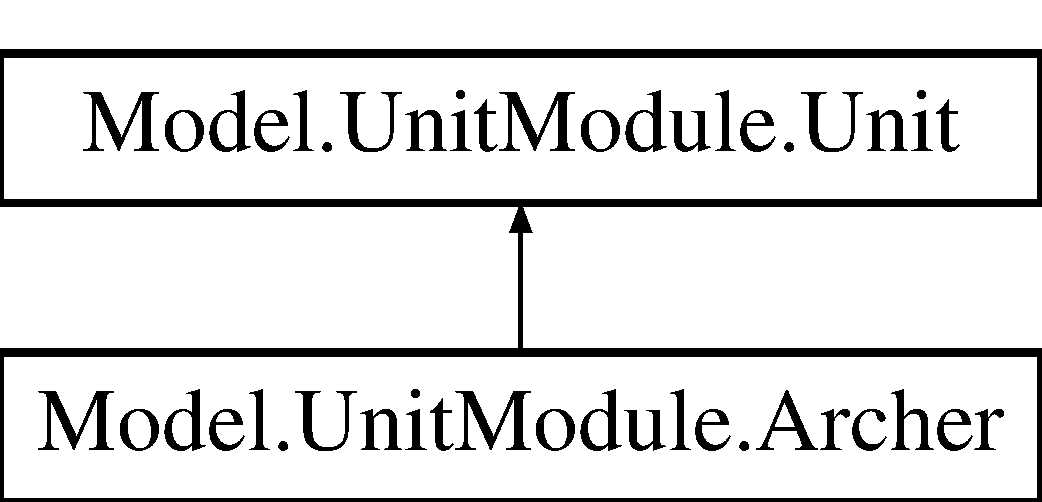
\includegraphics[height=2.000000cm]{class_model_1_1_unit_module_1_1_archer}
\end{center}
\end{figure}
\subsection*{Public Member Functions}
\begin{DoxyCompactItemize}
\item 
\hyperlink{class_model_1_1_unit_module_1_1_archer_acb9f7b98dd16e29be30ee2fd97ce0cbc}{Archer} (Texture2D sprite\+Image, \hyperlink{class_model_1_1_button}{Button}\mbox{[}$\,$\mbox{]} unit\+Buttons, Texture2D char\+Info, Texture2D char\+Attack\+Info, Vector2 coordinates, Texture2D health\+Bar)
\item 
void \hyperlink{class_model_1_1_unit_module_1_1_archer_acd305143313040a061b7482039c7a9b6}{set\+Initial\+Stats} ()
\item 
int \hyperlink{class_model_1_1_unit_module_1_1_archer_a54970d1557f24e41507c5bd056ac1f03}{get\+Movability} ()
\item 
int \mbox{[}$\,$\mbox{]} \hyperlink{class_model_1_1_unit_module_1_1_archer_a1b339759429e0a031aadf2b3e2505e66}{get\+Stats} ()
\item 
\hyperlink{interface_model_1_1_weapon_module_1_1_weapon}{Weapon} \mbox{[}$\,$\mbox{]} \hyperlink{class_model_1_1_unit_module_1_1_archer_a470c428226089a8872e1bc3901388196}{get\+Equipable\+Weapons} ()
\item 
\hyperlink{namespace_model_1_1_unit_module_aba9769f408747bf38d0d8adca8f68c98}{Unit\+Type} \hyperlink{class_model_1_1_unit_module_1_1_archer_a2211d99610a907939dac87cb75c3afb1}{get\+Class} ()
\item 
Texture2D \hyperlink{class_model_1_1_unit_module_1_1_archer_a2a400bdeef5aaaa34ffe6428ecaaf2c2}{get\+Sprite\+Image} ()
\item 
Texture2D \hyperlink{class_model_1_1_unit_module_1_1_archer_a6890f21c7dd51b1e22fed4047906f85f}{get\+Button\+Image} (\hyperlink{namespace_model_ac76b3489c9d704f49912608bd36cd0e7}{Button\+Type} button\+Type)
\item 
bool \hyperlink{class_model_1_1_unit_module_1_1_archer_ae3a17a1d3f60e9e35e0d25c45158a8eb}{is\+Button\+Active} (\hyperlink{namespace_model_ac76b3489c9d704f49912608bd36cd0e7}{Button\+Type} button\+Type)
\item 
Texture2D \hyperlink{class_model_1_1_unit_module_1_1_archer_acfcb3e900ee60c0bd9ed800efc9abcac}{get\+Char\+Info} ()
\item 
Texture2D \hyperlink{class_model_1_1_unit_module_1_1_archer_aafb7e46f581d1710a16d054dfef03ddf}{get\+Char\+Attack\+Info} ()
\item 
\hyperlink{class_model_1_1_button}{Button} \mbox{[}$\,$\mbox{]} \hyperlink{class_model_1_1_unit_module_1_1_archer_a8306cd02babf69626ce85bed7e76d089}{get\+Buttons} ()
\item 
\hyperlink{class_model_1_1_button}{Button} \hyperlink{class_model_1_1_unit_module_1_1_archer_af4d544ecd34e57d071a129fb7d0f155d}{get\+Button\+Type} (\hyperlink{namespace_model_ac76b3489c9d704f49912608bd36cd0e7}{Button\+Type} button\+Type)
\item 
void \hyperlink{class_model_1_1_unit_module_1_1_archer_ad1e9c182bc11a0ea83134421a24c7987}{set\+Button\+Coordinates} (Vector2 pixel\+Coordinates)
\item 
Rectangle \hyperlink{class_model_1_1_unit_module_1_1_archer_ac116699a7276c0549d2be5c3998d8813}{get\+Current\+Frame} ()
\item 
Texture2D \hyperlink{class_model_1_1_unit_module_1_1_archer_a113518d26ecdbf45aca30fed1f884b3b}{get\+Health\+Bar} ()
\item 
int \hyperlink{class_model_1_1_unit_module_1_1_archer_abbb5c6501863bea35613df66a094b490}{get\+Max\+Hp} ()
\end{DoxyCompactItemize}
\subsection*{Properties}
\begin{DoxyCompactItemize}
\item 
bool \hyperlink{class_model_1_1_unit_module_1_1_archer_a20bece941fa5cf234326fb10d09f92e0}{Alive}\hspace{0.3cm}{\ttfamily  \mbox{[}get, set\mbox{]}}
\item 
int \hyperlink{class_model_1_1_unit_module_1_1_archer_ae944f41f10572d4a183229726950eeec}{Speed}\hspace{0.3cm}{\ttfamily  \mbox{[}get, set\mbox{]}}
\item 
int \hyperlink{class_model_1_1_unit_module_1_1_archer_a6b001252ea85b654e1c85fa47efd9d7b}{Def}\hspace{0.3cm}{\ttfamily  \mbox{[}get, set\mbox{]}}
\item 
int \hyperlink{class_model_1_1_unit_module_1_1_archer_ae930922325e02ed61ff2be93d8ee24b0}{Res}\hspace{0.3cm}{\ttfamily  \mbox{[}get, set\mbox{]}}
\item 
int \hyperlink{class_model_1_1_unit_module_1_1_archer_a8f0956dcf4b5053754652649e72655e2}{Level}\hspace{0.3cm}{\ttfamily  \mbox{[}get, set\mbox{]}}
\item 
\hyperlink{interface_model_1_1_weapon_module_1_1_weapon}{Weapon} \hyperlink{class_model_1_1_unit_module_1_1_archer_aff2e126518d4eb4e64a06ac44542fefe}{equipped\+Weapon}\hspace{0.3cm}{\ttfamily  \mbox{[}get, set\mbox{]}}
\item 
int \hyperlink{class_model_1_1_unit_module_1_1_archer_adfb64d60ccce91e614bdbf834feff655}{current\+Frame}\hspace{0.3cm}{\ttfamily  \mbox{[}get, set\mbox{]}}
\item 
int \hyperlink{class_model_1_1_unit_module_1_1_archer_a4dd2b6dcabc11e4d5fcfa0856a9f85aa}{Str}\hspace{0.3cm}{\ttfamily  \mbox{[}get, set\mbox{]}}
\item 
int \hyperlink{class_model_1_1_unit_module_1_1_archer_ae003038905be807ec42d56ac979b1369}{Int}\hspace{0.3cm}{\ttfamily  \mbox{[}get, set\mbox{]}}
\item 
int \hyperlink{class_model_1_1_unit_module_1_1_archer_ad2b77a7ad32761658101c22051c35f7e}{Skill}\hspace{0.3cm}{\ttfamily  \mbox{[}get, set\mbox{]}}
\item 
int \hyperlink{class_model_1_1_unit_module_1_1_archer_aa98508c9166b0d5661952efc2577e2f7}{Hp}\hspace{0.3cm}{\ttfamily  \mbox{[}get, set\mbox{]}}
\item 
Tuple$<$ int, int $>$ \hyperlink{class_model_1_1_unit_module_1_1_archer_a0038f1b30e38e431dee388f6fdf8b6d7}{Position}\hspace{0.3cm}{\ttfamily  \mbox{[}get, set\mbox{]}}
\item 
Vector2 \hyperlink{class_model_1_1_unit_module_1_1_archer_abe69c6c957abd5c25c7c52576faa015c}{Pixel\+Coordinates}\hspace{0.3cm}{\ttfamily  \mbox{[}get, set\mbox{]}}
\end{DoxyCompactItemize}


\subsection{Detailed Description}
The \hyperlink{class_model_1_1_unit_module_1_1_archer}{Archer} model class, extends \hyperlink{interface_model_1_1_unit_module_1_1_unit}{Unit}. This unit has a high skill and speed, and excels in dealing accurate ranged, high critical, physical attacks, but suffers from overall defense against physical attacks. 



\subsection{Constructor \& Destructor Documentation}
\hypertarget{class_model_1_1_unit_module_1_1_archer_acb9f7b98dd16e29be30ee2fd97ce0cbc}{}\label{class_model_1_1_unit_module_1_1_archer_acb9f7b98dd16e29be30ee2fd97ce0cbc} 
\index{Model\+::\+Unit\+Module\+::\+Archer@{Model\+::\+Unit\+Module\+::\+Archer}!Archer@{Archer}}
\index{Archer@{Archer}!Model\+::\+Unit\+Module\+::\+Archer@{Model\+::\+Unit\+Module\+::\+Archer}}
\subsubsection{\texorpdfstring{Archer()}{Archer()}}
{\footnotesize\ttfamily Model.\+Unit\+Module.\+Archer.\+Archer (\begin{DoxyParamCaption}\item[{Texture2D}]{sprite\+Image,  }\item[{\hyperlink{class_model_1_1_button}{Button} \mbox{[}$\,$\mbox{]}}]{unit\+Buttons,  }\item[{Texture2D}]{char\+Info,  }\item[{Texture2D}]{char\+Attack\+Info,  }\item[{Vector2}]{coordinates,  }\item[{Texture2D}]{health\+Bar }\end{DoxyParamCaption})\hspace{0.3cm}{\ttfamily [inline]}}

The constructor for \hyperlink{interface_model_1_1_unit_module_1_1_unit}{Unit} \hyperlink{class_model_1_1_unit_module_1_1_archer}{Archer}. Stores all relevent data in model. 
\begin{DoxyParams}{Parameters}
{\em sprite\+Image} & The character sprite texture. \\
\hline
{\em unit\+Buttons} & The Texture2D Array containing all the different textures for each button. \\
\hline
{\em char\+Info} & The character info popup texture. \\
\hline
{\em char\+Attack\+Info} & The character attack menu popup texture. \\
\hline
{\em coordinates} & The unit\textquotesingle{}s current vector coordinate on screen. \\
\hline
{\em player} & The player of which the unit belongs to. \\
\hline
\end{DoxyParams}


\subsection{Member Function Documentation}
\hypertarget{class_model_1_1_unit_module_1_1_archer_a6890f21c7dd51b1e22fed4047906f85f}{}\label{class_model_1_1_unit_module_1_1_archer_a6890f21c7dd51b1e22fed4047906f85f} 
\index{Model\+::\+Unit\+Module\+::\+Archer@{Model\+::\+Unit\+Module\+::\+Archer}!get\+Button\+Image@{get\+Button\+Image}}
\index{get\+Button\+Image@{get\+Button\+Image}!Model\+::\+Unit\+Module\+::\+Archer@{Model\+::\+Unit\+Module\+::\+Archer}}
\subsubsection{\texorpdfstring{get\+Button\+Image()}{getButtonImage()}}
{\footnotesize\ttfamily Texture2D Model.\+Unit\+Module.\+Archer.\+get\+Button\+Image (\begin{DoxyParamCaption}\item[{\hyperlink{namespace_model_ac76b3489c9d704f49912608bd36cd0e7}{Button\+Type}}]{button\+Type }\end{DoxyParamCaption})\hspace{0.3cm}{\ttfamily [inline]}}

This method returns the texture associated with the buntton\+Type passed in, by going through a switch case and matching it. 
\begin{DoxyParams}{Parameters}
{\em button\+Type} & The buttontype that was clicked. \\
\hline
\end{DoxyParams}


Implements \hyperlink{interface_model_1_1_unit_module_1_1_unit_ac8e47a3f8d13fe8a719f962a3ee9ee46}{Model.\+Unit\+Module.\+Unit}.

\hypertarget{class_model_1_1_unit_module_1_1_archer_a8306cd02babf69626ce85bed7e76d089}{}\label{class_model_1_1_unit_module_1_1_archer_a8306cd02babf69626ce85bed7e76d089} 
\index{Model\+::\+Unit\+Module\+::\+Archer@{Model\+::\+Unit\+Module\+::\+Archer}!get\+Buttons@{get\+Buttons}}
\index{get\+Buttons@{get\+Buttons}!Model\+::\+Unit\+Module\+::\+Archer@{Model\+::\+Unit\+Module\+::\+Archer}}
\subsubsection{\texorpdfstring{get\+Buttons()}{getButtons()}}
{\footnotesize\ttfamily \hyperlink{class_model_1_1_button}{Button} \mbox{[}$\,$\mbox{]} Model.\+Unit\+Module.\+Archer.\+get\+Buttons (\begin{DoxyParamCaption}{ }\end{DoxyParamCaption})\hspace{0.3cm}{\ttfamily [inline]}}

Returns the dropdown menu buttons of the unit. 

Implements \hyperlink{interface_model_1_1_unit_module_1_1_unit_a5256d2141e9c59e0454e47ac65246bda}{Model.\+Unit\+Module.\+Unit}.

\hypertarget{class_model_1_1_unit_module_1_1_archer_af4d544ecd34e57d071a129fb7d0f155d}{}\label{class_model_1_1_unit_module_1_1_archer_af4d544ecd34e57d071a129fb7d0f155d} 
\index{Model\+::\+Unit\+Module\+::\+Archer@{Model\+::\+Unit\+Module\+::\+Archer}!get\+Button\+Type@{get\+Button\+Type}}
\index{get\+Button\+Type@{get\+Button\+Type}!Model\+::\+Unit\+Module\+::\+Archer@{Model\+::\+Unit\+Module\+::\+Archer}}
\subsubsection{\texorpdfstring{get\+Button\+Type()}{getButtonType()}}
{\footnotesize\ttfamily \hyperlink{class_model_1_1_button}{Button} Model.\+Unit\+Module.\+Archer.\+get\+Button\+Type (\begin{DoxyParamCaption}\item[{\hyperlink{namespace_model_ac76b3489c9d704f49912608bd36cd0e7}{Button\+Type}}]{button\+Type }\end{DoxyParamCaption})\hspace{0.3cm}{\ttfamily [inline]}}

This method takes in the button\+Type enum, then returns the object associated with that enum. 
\begin{DoxyParams}{Parameters}
{\em button\+Type} & The button to return (Move, Attack, Item, Wait, and attack confirm). \\
\hline
\end{DoxyParams}


Implements \hyperlink{interface_model_1_1_unit_module_1_1_unit_a6e9528d09bca7702fe99cc95135ede36}{Model.\+Unit\+Module.\+Unit}.

\hypertarget{class_model_1_1_unit_module_1_1_archer_aafb7e46f581d1710a16d054dfef03ddf}{}\label{class_model_1_1_unit_module_1_1_archer_aafb7e46f581d1710a16d054dfef03ddf} 
\index{Model\+::\+Unit\+Module\+::\+Archer@{Model\+::\+Unit\+Module\+::\+Archer}!get\+Char\+Attack\+Info@{get\+Char\+Attack\+Info}}
\index{get\+Char\+Attack\+Info@{get\+Char\+Attack\+Info}!Model\+::\+Unit\+Module\+::\+Archer@{Model\+::\+Unit\+Module\+::\+Archer}}
\subsubsection{\texorpdfstring{get\+Char\+Attack\+Info()}{getCharAttackInfo()}}
{\footnotesize\ttfamily Texture2D Model.\+Unit\+Module.\+Archer.\+get\+Char\+Attack\+Info (\begin{DoxyParamCaption}{ }\end{DoxyParamCaption})\hspace{0.3cm}{\ttfamily [inline]}}

Returns the char attack info screen texture. 

Implements \hyperlink{interface_model_1_1_unit_module_1_1_unit_a7c89d9a1dc648b556b7e57cdcdbf2930}{Model.\+Unit\+Module.\+Unit}.

\hypertarget{class_model_1_1_unit_module_1_1_archer_acfcb3e900ee60c0bd9ed800efc9abcac}{}\label{class_model_1_1_unit_module_1_1_archer_acfcb3e900ee60c0bd9ed800efc9abcac} 
\index{Model\+::\+Unit\+Module\+::\+Archer@{Model\+::\+Unit\+Module\+::\+Archer}!get\+Char\+Info@{get\+Char\+Info}}
\index{get\+Char\+Info@{get\+Char\+Info}!Model\+::\+Unit\+Module\+::\+Archer@{Model\+::\+Unit\+Module\+::\+Archer}}
\subsubsection{\texorpdfstring{get\+Char\+Info()}{getCharInfo()}}
{\footnotesize\ttfamily Texture2D Model.\+Unit\+Module.\+Archer.\+get\+Char\+Info (\begin{DoxyParamCaption}{ }\end{DoxyParamCaption})\hspace{0.3cm}{\ttfamily [inline]}}

Returns the char info screen texture. 

Implements \hyperlink{interface_model_1_1_unit_module_1_1_unit_a4e2aeae552d85c8938e609729bcd1a44}{Model.\+Unit\+Module.\+Unit}.

\hypertarget{class_model_1_1_unit_module_1_1_archer_a2211d99610a907939dac87cb75c3afb1}{}\label{class_model_1_1_unit_module_1_1_archer_a2211d99610a907939dac87cb75c3afb1} 
\index{Model\+::\+Unit\+Module\+::\+Archer@{Model\+::\+Unit\+Module\+::\+Archer}!get\+Class@{get\+Class}}
\index{get\+Class@{get\+Class}!Model\+::\+Unit\+Module\+::\+Archer@{Model\+::\+Unit\+Module\+::\+Archer}}
\subsubsection{\texorpdfstring{get\+Class()}{getClass()}}
{\footnotesize\ttfamily \hyperlink{namespace_model_1_1_unit_module_aba9769f408747bf38d0d8adca8f68c98}{Unit\+Type} Model.\+Unit\+Module.\+Archer.\+get\+Class (\begin{DoxyParamCaption}{ }\end{DoxyParamCaption})\hspace{0.3cm}{\ttfamily [inline]}}

Returns the unit\textquotesingle{}s class. 

Implements \hyperlink{interface_model_1_1_unit_module_1_1_unit_a84dbb2982a68ec530e53662d747da9fa}{Model.\+Unit\+Module.\+Unit}.

\hypertarget{class_model_1_1_unit_module_1_1_archer_ac116699a7276c0549d2be5c3998d8813}{}\label{class_model_1_1_unit_module_1_1_archer_ac116699a7276c0549d2be5c3998d8813} 
\index{Model\+::\+Unit\+Module\+::\+Archer@{Model\+::\+Unit\+Module\+::\+Archer}!get\+Current\+Frame@{get\+Current\+Frame}}
\index{get\+Current\+Frame@{get\+Current\+Frame}!Model\+::\+Unit\+Module\+::\+Archer@{Model\+::\+Unit\+Module\+::\+Archer}}
\subsubsection{\texorpdfstring{get\+Current\+Frame()}{getCurrentFrame()}}
{\footnotesize\ttfamily Rectangle Model.\+Unit\+Module.\+Archer.\+get\+Current\+Frame (\begin{DoxyParamCaption}{ }\end{DoxyParamCaption})\hspace{0.3cm}{\ttfamily [inline]}}

returns the current sprite frame in animation sequence. The rectangle starts at current\+Frame $\ast$ 32, where 32 is the sprite sheet offset between frames, and is 32 high and wide. ~\newline
 {\bfseries Exceptions\+:} ~\newline
 -\/\+Assumes that each sprite frame is 32pixels wide. 

Implements \hyperlink{interface_model_1_1_unit_module_1_1_unit_accb79e396c6066707f2d11f63e3fdd99}{Model.\+Unit\+Module.\+Unit}.

\hypertarget{class_model_1_1_unit_module_1_1_archer_a470c428226089a8872e1bc3901388196}{}\label{class_model_1_1_unit_module_1_1_archer_a470c428226089a8872e1bc3901388196} 
\index{Model\+::\+Unit\+Module\+::\+Archer@{Model\+::\+Unit\+Module\+::\+Archer}!get\+Equipable\+Weapons@{get\+Equipable\+Weapons}}
\index{get\+Equipable\+Weapons@{get\+Equipable\+Weapons}!Model\+::\+Unit\+Module\+::\+Archer@{Model\+::\+Unit\+Module\+::\+Archer}}
\subsubsection{\texorpdfstring{get\+Equipable\+Weapons()}{getEquipableWeapons()}}
{\footnotesize\ttfamily \hyperlink{interface_model_1_1_weapon_module_1_1_weapon}{Weapon} \mbox{[}$\,$\mbox{]} Model.\+Unit\+Module.\+Archer.\+get\+Equipable\+Weapons (\begin{DoxyParamCaption}{ }\end{DoxyParamCaption})\hspace{0.3cm}{\ttfamily [inline]}}

Returns the list weapons the unit can equip (T\+O\+DO). 

Implements \hyperlink{interface_model_1_1_unit_module_1_1_unit_a7b64e60f28d516a5fb4e28a9b7cd8eec}{Model.\+Unit\+Module.\+Unit}.

\hypertarget{class_model_1_1_unit_module_1_1_archer_a113518d26ecdbf45aca30fed1f884b3b}{}\label{class_model_1_1_unit_module_1_1_archer_a113518d26ecdbf45aca30fed1f884b3b} 
\index{Model\+::\+Unit\+Module\+::\+Archer@{Model\+::\+Unit\+Module\+::\+Archer}!get\+Health\+Bar@{get\+Health\+Bar}}
\index{get\+Health\+Bar@{get\+Health\+Bar}!Model\+::\+Unit\+Module\+::\+Archer@{Model\+::\+Unit\+Module\+::\+Archer}}
\subsubsection{\texorpdfstring{get\+Health\+Bar()}{getHealthBar()}}
{\footnotesize\ttfamily Texture2D Model.\+Unit\+Module.\+Archer.\+get\+Health\+Bar (\begin{DoxyParamCaption}{ }\end{DoxyParamCaption})\hspace{0.3cm}{\ttfamily [inline]}}

Returns the healthbar texture. 

Implements \hyperlink{interface_model_1_1_unit_module_1_1_unit_a5be18da3857bb22525feb89dd49b76b1}{Model.\+Unit\+Module.\+Unit}.

\hypertarget{class_model_1_1_unit_module_1_1_archer_abbb5c6501863bea35613df66a094b490}{}\label{class_model_1_1_unit_module_1_1_archer_abbb5c6501863bea35613df66a094b490} 
\index{Model\+::\+Unit\+Module\+::\+Archer@{Model\+::\+Unit\+Module\+::\+Archer}!get\+Max\+Hp@{get\+Max\+Hp}}
\index{get\+Max\+Hp@{get\+Max\+Hp}!Model\+::\+Unit\+Module\+::\+Archer@{Model\+::\+Unit\+Module\+::\+Archer}}
\subsubsection{\texorpdfstring{get\+Max\+Hp()}{getMaxHp()}}
{\footnotesize\ttfamily int Model.\+Unit\+Module.\+Archer.\+get\+Max\+Hp (\begin{DoxyParamCaption}{ }\end{DoxyParamCaption})\hspace{0.3cm}{\ttfamily [inline]}}

Returns the character\textquotesingle{}s max HP. 

Implements \hyperlink{interface_model_1_1_unit_module_1_1_unit_adee907637c0ce8487149ae4549fb4cf1}{Model.\+Unit\+Module.\+Unit}.

\hypertarget{class_model_1_1_unit_module_1_1_archer_a54970d1557f24e41507c5bd056ac1f03}{}\label{class_model_1_1_unit_module_1_1_archer_a54970d1557f24e41507c5bd056ac1f03} 
\index{Model\+::\+Unit\+Module\+::\+Archer@{Model\+::\+Unit\+Module\+::\+Archer}!get\+Movability@{get\+Movability}}
\index{get\+Movability@{get\+Movability}!Model\+::\+Unit\+Module\+::\+Archer@{Model\+::\+Unit\+Module\+::\+Archer}}
\subsubsection{\texorpdfstring{get\+Movability()}{getMovability()}}
{\footnotesize\ttfamily int Model.\+Unit\+Module.\+Archer.\+get\+Movability (\begin{DoxyParamCaption}{ }\end{DoxyParamCaption})\hspace{0.3cm}{\ttfamily [inline]}}

Returns the unit\textquotesingle{}s movability range on grid (number of spaces the unit can move in one turn). ~\newline
{\bfseries Exceptions\+:} ~\newline
 -\/\+Negative movement will be treated as 0 in path finding algorithm. 

Implements \hyperlink{interface_model_1_1_unit_module_1_1_unit_a670aae31f46980c871774352f5fe3a3f}{Model.\+Unit\+Module.\+Unit}.

\hypertarget{class_model_1_1_unit_module_1_1_archer_a2a400bdeef5aaaa34ffe6428ecaaf2c2}{}\label{class_model_1_1_unit_module_1_1_archer_a2a400bdeef5aaaa34ffe6428ecaaf2c2} 
\index{Model\+::\+Unit\+Module\+::\+Archer@{Model\+::\+Unit\+Module\+::\+Archer}!get\+Sprite\+Image@{get\+Sprite\+Image}}
\index{get\+Sprite\+Image@{get\+Sprite\+Image}!Model\+::\+Unit\+Module\+::\+Archer@{Model\+::\+Unit\+Module\+::\+Archer}}
\subsubsection{\texorpdfstring{get\+Sprite\+Image()}{getSpriteImage()}}
{\footnotesize\ttfamily Texture2D Model.\+Unit\+Module.\+Archer.\+get\+Sprite\+Image (\begin{DoxyParamCaption}{ }\end{DoxyParamCaption})\hspace{0.3cm}{\ttfamily [inline]}}

Returns the sprite image of the unit. 

Implements \hyperlink{interface_model_1_1_unit_module_1_1_unit_a797013e0463ea2e8c9ae8171f7d305f0}{Model.\+Unit\+Module.\+Unit}.

\hypertarget{class_model_1_1_unit_module_1_1_archer_a1b339759429e0a031aadf2b3e2505e66}{}\label{class_model_1_1_unit_module_1_1_archer_a1b339759429e0a031aadf2b3e2505e66} 
\index{Model\+::\+Unit\+Module\+::\+Archer@{Model\+::\+Unit\+Module\+::\+Archer}!get\+Stats@{get\+Stats}}
\index{get\+Stats@{get\+Stats}!Model\+::\+Unit\+Module\+::\+Archer@{Model\+::\+Unit\+Module\+::\+Archer}}
\subsubsection{\texorpdfstring{get\+Stats()}{getStats()}}
{\footnotesize\ttfamily int \mbox{[}$\,$\mbox{]} Model.\+Unit\+Module.\+Archer.\+get\+Stats (\begin{DoxyParamCaption}{ }\end{DoxyParamCaption})\hspace{0.3cm}{\ttfamily [inline]}}

Returns all stats as an array, where the index in array corresponds to stats in this order\+: ~\newline
 Level, Strength, Int, Skill, Speed, Def, Res. 

Implements \hyperlink{interface_model_1_1_unit_module_1_1_unit_a32890c6e0bf19a58dde71cc4240576a8}{Model.\+Unit\+Module.\+Unit}.

\hypertarget{class_model_1_1_unit_module_1_1_archer_ae3a17a1d3f60e9e35e0d25c45158a8eb}{}\label{class_model_1_1_unit_module_1_1_archer_ae3a17a1d3f60e9e35e0d25c45158a8eb} 
\index{Model\+::\+Unit\+Module\+::\+Archer@{Model\+::\+Unit\+Module\+::\+Archer}!is\+Button\+Active@{is\+Button\+Active}}
\index{is\+Button\+Active@{is\+Button\+Active}!Model\+::\+Unit\+Module\+::\+Archer@{Model\+::\+Unit\+Module\+::\+Archer}}
\subsubsection{\texorpdfstring{is\+Button\+Active()}{isButtonActive()}}
{\footnotesize\ttfamily bool Model.\+Unit\+Module.\+Archer.\+is\+Button\+Active (\begin{DoxyParamCaption}\item[{\hyperlink{namespace_model_ac76b3489c9d704f49912608bd36cd0e7}{Button\+Type}}]{button\+Type }\end{DoxyParamCaption})\hspace{0.3cm}{\ttfamily [inline]}}

This method takes in the button\+Type specified, and checks if that button is currently active by calling the getter in button. 
\begin{DoxyParams}{Parameters}
{\em button\+Type} & The buttontype that was clicked. \\
\hline
\end{DoxyParams}


Implements \hyperlink{interface_model_1_1_unit_module_1_1_unit_a3931ef1523507e7261411dc79ee4e4af}{Model.\+Unit\+Module.\+Unit}.

\hypertarget{class_model_1_1_unit_module_1_1_archer_ad1e9c182bc11a0ea83134421a24c7987}{}\label{class_model_1_1_unit_module_1_1_archer_ad1e9c182bc11a0ea83134421a24c7987} 
\index{Model\+::\+Unit\+Module\+::\+Archer@{Model\+::\+Unit\+Module\+::\+Archer}!set\+Button\+Coordinates@{set\+Button\+Coordinates}}
\index{set\+Button\+Coordinates@{set\+Button\+Coordinates}!Model\+::\+Unit\+Module\+::\+Archer@{Model\+::\+Unit\+Module\+::\+Archer}}
\subsubsection{\texorpdfstring{set\+Button\+Coordinates()}{setButtonCoordinates()}}
{\footnotesize\ttfamily void Model.\+Unit\+Module.\+Archer.\+set\+Button\+Coordinates (\begin{DoxyParamCaption}\item[{Vector2}]{pixel\+Coordinates }\end{DoxyParamCaption})\hspace{0.3cm}{\ttfamily [inline]}}

Sets the coordinates of menu buttons. One for loop will position the main Drop Down menu (potentailly containing attack, move, item and wait directly 32 pixels to the right of unit (so the tile to right of unit) , and for each active button, increment it downwards by 32 pixels (height of each button). The second for loop is similiar and is for the inventory menu buttons, except it starts 160 pixels offsetted to right (to the right of the main drop down menu). 
\begin{DoxyParams}{Parameters}
{\em pixel\+Coordinates} & The pixel coordinate of the button. \\
\hline
\end{DoxyParams}


Implements \hyperlink{interface_model_1_1_unit_module_1_1_unit_ad48776b3bd231bf80d2eec87b7498302}{Model.\+Unit\+Module.\+Unit}.

\hypertarget{class_model_1_1_unit_module_1_1_archer_acd305143313040a061b7482039c7a9b6}{}\label{class_model_1_1_unit_module_1_1_archer_acd305143313040a061b7482039c7a9b6} 
\index{Model\+::\+Unit\+Module\+::\+Archer@{Model\+::\+Unit\+Module\+::\+Archer}!set\+Initial\+Stats@{set\+Initial\+Stats}}
\index{set\+Initial\+Stats@{set\+Initial\+Stats}!Model\+::\+Unit\+Module\+::\+Archer@{Model\+::\+Unit\+Module\+::\+Archer}}
\subsubsection{\texorpdfstring{set\+Initial\+Stats()}{setInitialStats()}}
{\footnotesize\ttfamily void Model.\+Unit\+Module.\+Archer.\+set\+Initial\+Stats (\begin{DoxyParamCaption}{ }\end{DoxyParamCaption})\hspace{0.3cm}{\ttfamily [inline]}}

Sets the initial unit stats before modifiers. 

Implements \hyperlink{interface_model_1_1_unit_module_1_1_unit_a3b67c1b9e929a9f7d4191de20996220a}{Model.\+Unit\+Module.\+Unit}.



\subsection{Property Documentation}
\hypertarget{class_model_1_1_unit_module_1_1_archer_a20bece941fa5cf234326fb10d09f92e0}{}\label{class_model_1_1_unit_module_1_1_archer_a20bece941fa5cf234326fb10d09f92e0} 
\index{Model\+::\+Unit\+Module\+::\+Archer@{Model\+::\+Unit\+Module\+::\+Archer}!Alive@{Alive}}
\index{Alive@{Alive}!Model\+::\+Unit\+Module\+::\+Archer@{Model\+::\+Unit\+Module\+::\+Archer}}
\subsubsection{\texorpdfstring{Alive}{Alive}}
{\footnotesize\ttfamily bool Model.\+Unit\+Module.\+Archer.\+Alive\hspace{0.3cm}{\ttfamily [get]}, {\ttfamily [set]}}

Sets and returns whether or not unit is alive. \hypertarget{class_model_1_1_unit_module_1_1_archer_adfb64d60ccce91e614bdbf834feff655}{}\label{class_model_1_1_unit_module_1_1_archer_adfb64d60ccce91e614bdbf834feff655} 
\index{Model\+::\+Unit\+Module\+::\+Archer@{Model\+::\+Unit\+Module\+::\+Archer}!current\+Frame@{current\+Frame}}
\index{current\+Frame@{current\+Frame}!Model\+::\+Unit\+Module\+::\+Archer@{Model\+::\+Unit\+Module\+::\+Archer}}
\subsubsection{\texorpdfstring{current\+Frame}{currentFrame}}
{\footnotesize\ttfamily int Model.\+Unit\+Module.\+Archer.\+current\+Frame\hspace{0.3cm}{\ttfamily [get]}, {\ttfamily [set]}}

Gets and sets current frame the sprite is on. \hypertarget{class_model_1_1_unit_module_1_1_archer_a6b001252ea85b654e1c85fa47efd9d7b}{}\label{class_model_1_1_unit_module_1_1_archer_a6b001252ea85b654e1c85fa47efd9d7b} 
\index{Model\+::\+Unit\+Module\+::\+Archer@{Model\+::\+Unit\+Module\+::\+Archer}!Def@{Def}}
\index{Def@{Def}!Model\+::\+Unit\+Module\+::\+Archer@{Model\+::\+Unit\+Module\+::\+Archer}}
\subsubsection{\texorpdfstring{Def}{Def}}
{\footnotesize\ttfamily int Model.\+Unit\+Module.\+Archer.\+Def\hspace{0.3cm}{\ttfamily [get]}, {\ttfamily [set]}}

Sets and returns a unit\textquotesingle{}s Defense. ~\newline
 {\bfseries Exceptions\+:} ~\newline
 -\/\+Negative defense will result in an attacker doing more damage than their attack. \hypertarget{class_model_1_1_unit_module_1_1_archer_aff2e126518d4eb4e64a06ac44542fefe}{}\label{class_model_1_1_unit_module_1_1_archer_aff2e126518d4eb4e64a06ac44542fefe} 
\index{Model\+::\+Unit\+Module\+::\+Archer@{Model\+::\+Unit\+Module\+::\+Archer}!equipped\+Weapon@{equipped\+Weapon}}
\index{equipped\+Weapon@{equipped\+Weapon}!Model\+::\+Unit\+Module\+::\+Archer@{Model\+::\+Unit\+Module\+::\+Archer}}
\subsubsection{\texorpdfstring{equipped\+Weapon}{equippedWeapon}}
{\footnotesize\ttfamily \hyperlink{interface_model_1_1_weapon_module_1_1_weapon}{Weapon} Model.\+Unit\+Module.\+Archer.\+equipped\+Weapon\hspace{0.3cm}{\ttfamily [get]}, {\ttfamily [set]}}

Gets and sets the unit is currently equipping. \hypertarget{class_model_1_1_unit_module_1_1_archer_aa98508c9166b0d5661952efc2577e2f7}{}\label{class_model_1_1_unit_module_1_1_archer_aa98508c9166b0d5661952efc2577e2f7} 
\index{Model\+::\+Unit\+Module\+::\+Archer@{Model\+::\+Unit\+Module\+::\+Archer}!Hp@{Hp}}
\index{Hp@{Hp}!Model\+::\+Unit\+Module\+::\+Archer@{Model\+::\+Unit\+Module\+::\+Archer}}
\subsubsection{\texorpdfstring{Hp}{Hp}}
{\footnotesize\ttfamily int Model.\+Unit\+Module.\+Archer.\+Hp\hspace{0.3cm}{\ttfamily [get]}, {\ttfamily [set]}}

Sets and get a unit\textquotesingle{}s HP. Should HP fall under 0, \hyperlink{interface_model_1_1_unit_module_1_1_unit}{Unit}\textquotesingle{}s Alive Boolean should change to false. \hypertarget{class_model_1_1_unit_module_1_1_archer_ae003038905be807ec42d56ac979b1369}{}\label{class_model_1_1_unit_module_1_1_archer_ae003038905be807ec42d56ac979b1369} 
\index{Model\+::\+Unit\+Module\+::\+Archer@{Model\+::\+Unit\+Module\+::\+Archer}!Int@{Int}}
\index{Int@{Int}!Model\+::\+Unit\+Module\+::\+Archer@{Model\+::\+Unit\+Module\+::\+Archer}}
\subsubsection{\texorpdfstring{Int}{Int}}
{\footnotesize\ttfamily int Model.\+Unit\+Module.\+Archer.\+Int\hspace{0.3cm}{\ttfamily [get]}, {\ttfamily [set]}}

Sets and gets the new intelligence value. ~\newline
 Gets the effective intelligence -\/$>$ \hyperlink{interface_model_1_1_unit_module_1_1_unit}{Unit} intelligence + weapon intelligence ~\newline
 {\bfseries Exceptions\+:} ~\newline
 -\/\+Negative strength will be treated as 0 in damage calculation, as damage dealt can not be negative. \hypertarget{class_model_1_1_unit_module_1_1_archer_a8f0956dcf4b5053754652649e72655e2}{}\label{class_model_1_1_unit_module_1_1_archer_a8f0956dcf4b5053754652649e72655e2} 
\index{Model\+::\+Unit\+Module\+::\+Archer@{Model\+::\+Unit\+Module\+::\+Archer}!Level@{Level}}
\index{Level@{Level}!Model\+::\+Unit\+Module\+::\+Archer@{Model\+::\+Unit\+Module\+::\+Archer}}
\subsubsection{\texorpdfstring{Level}{Level}}
{\footnotesize\ttfamily int Model.\+Unit\+Module.\+Archer.\+Level\hspace{0.3cm}{\ttfamily [get]}, {\ttfamily [set]}}

Sets and returns a unit\textquotesingle{}s Level. Currently does not have any use. \hypertarget{class_model_1_1_unit_module_1_1_archer_abe69c6c957abd5c25c7c52576faa015c}{}\label{class_model_1_1_unit_module_1_1_archer_abe69c6c957abd5c25c7c52576faa015c} 
\index{Model\+::\+Unit\+Module\+::\+Archer@{Model\+::\+Unit\+Module\+::\+Archer}!Pixel\+Coordinates@{Pixel\+Coordinates}}
\index{Pixel\+Coordinates@{Pixel\+Coordinates}!Model\+::\+Unit\+Module\+::\+Archer@{Model\+::\+Unit\+Module\+::\+Archer}}
\subsubsection{\texorpdfstring{Pixel\+Coordinates}{PixelCoordinates}}
{\footnotesize\ttfamily Vector2 Model.\+Unit\+Module.\+Archer.\+Pixel\+Coordinates\hspace{0.3cm}{\ttfamily [get]}, {\ttfamily [set]}}

Returns the pixel coordinate of the unit. ~\newline
 sets the pixel coordinate, and also sets Position (which is the tile location of that coordinate). ~\newline
{\bfseries Exceptions\+:} ~\newline
 -\/\+Dead units will still have a position, but won\textquotesingle{}t impact the rest of the game. \hypertarget{class_model_1_1_unit_module_1_1_archer_a0038f1b30e38e431dee388f6fdf8b6d7}{}\label{class_model_1_1_unit_module_1_1_archer_a0038f1b30e38e431dee388f6fdf8b6d7} 
\index{Model\+::\+Unit\+Module\+::\+Archer@{Model\+::\+Unit\+Module\+::\+Archer}!Position@{Position}}
\index{Position@{Position}!Model\+::\+Unit\+Module\+::\+Archer@{Model\+::\+Unit\+Module\+::\+Archer}}
\subsubsection{\texorpdfstring{Position}{Position}}
{\footnotesize\ttfamily Tuple$<$int, int$>$ Model.\+Unit\+Module.\+Archer.\+Position\hspace{0.3cm}{\ttfamily [get]}, {\ttfamily [set]}}

Gets and sets unit\textquotesingle{}s position by tile. The set also updates pixel\+Coordinate\textquotesingle{}s location by making that vector equivalent to position$\ast$32 (since each tile is 32x32). ~\newline
 {\bfseries Exceptions\+:} ~\newline
 -\/\+Dead units will still have a position, but won\textquotesingle{}t impact the rest of the game. \hypertarget{class_model_1_1_unit_module_1_1_archer_ae930922325e02ed61ff2be93d8ee24b0}{}\label{class_model_1_1_unit_module_1_1_archer_ae930922325e02ed61ff2be93d8ee24b0} 
\index{Model\+::\+Unit\+Module\+::\+Archer@{Model\+::\+Unit\+Module\+::\+Archer}!Res@{Res}}
\index{Res@{Res}!Model\+::\+Unit\+Module\+::\+Archer@{Model\+::\+Unit\+Module\+::\+Archer}}
\subsubsection{\texorpdfstring{Res}{Res}}
{\footnotesize\ttfamily int Model.\+Unit\+Module.\+Archer.\+Res\hspace{0.3cm}{\ttfamily [get]}, {\ttfamily [set]}}

Sets and returns a unit\textquotesingle{}s Resistance. ~\newline
 {\bfseries Exceptions\+:} ~\newline
 -\/\+Negative resistance will result in an attacker doing more damage than their intelligence. \hypertarget{class_model_1_1_unit_module_1_1_archer_ad2b77a7ad32761658101c22051c35f7e}{}\label{class_model_1_1_unit_module_1_1_archer_ad2b77a7ad32761658101c22051c35f7e} 
\index{Model\+::\+Unit\+Module\+::\+Archer@{Model\+::\+Unit\+Module\+::\+Archer}!Skill@{Skill}}
\index{Skill@{Skill}!Model\+::\+Unit\+Module\+::\+Archer@{Model\+::\+Unit\+Module\+::\+Archer}}
\subsubsection{\texorpdfstring{Skill}{Skill}}
{\footnotesize\ttfamily int Model.\+Unit\+Module.\+Archer.\+Skill\hspace{0.3cm}{\ttfamily [get]}, {\ttfamily [set]}}

Sets and gets the new skill value. ~\newline
 Gets the effective skill -\/$>$ \hyperlink{interface_model_1_1_unit_module_1_1_unit}{Unit} skill + weapon skill ~\newline
 {\bfseries Exceptions\+:} ~\newline
 -\/\+Negative skill will not result in an error, but will most likely result in a 0\% hit and crit rate. \hypertarget{class_model_1_1_unit_module_1_1_archer_ae944f41f10572d4a183229726950eeec}{}\label{class_model_1_1_unit_module_1_1_archer_ae944f41f10572d4a183229726950eeec} 
\index{Model\+::\+Unit\+Module\+::\+Archer@{Model\+::\+Unit\+Module\+::\+Archer}!Speed@{Speed}}
\index{Speed@{Speed}!Model\+::\+Unit\+Module\+::\+Archer@{Model\+::\+Unit\+Module\+::\+Archer}}
\subsubsection{\texorpdfstring{Speed}{Speed}}
{\footnotesize\ttfamily int Model.\+Unit\+Module.\+Archer.\+Speed\hspace{0.3cm}{\ttfamily [get]}, {\ttfamily [set]}}

Sets and returns a unit\textquotesingle{}s Speed. ~\newline
 {\bfseries Exceptions\+:} ~\newline
 -\/\+Negative skill will not result in an error as speed is only used for checking double attack boolean, which is binary. \hypertarget{class_model_1_1_unit_module_1_1_archer_a4dd2b6dcabc11e4d5fcfa0856a9f85aa}{}\label{class_model_1_1_unit_module_1_1_archer_a4dd2b6dcabc11e4d5fcfa0856a9f85aa} 
\index{Model\+::\+Unit\+Module\+::\+Archer@{Model\+::\+Unit\+Module\+::\+Archer}!Str@{Str}}
\index{Str@{Str}!Model\+::\+Unit\+Module\+::\+Archer@{Model\+::\+Unit\+Module\+::\+Archer}}
\subsubsection{\texorpdfstring{Str}{Str}}
{\footnotesize\ttfamily int Model.\+Unit\+Module.\+Archer.\+Str\hspace{0.3cm}{\ttfamily [get]}, {\ttfamily [set]}}

Sets and gets the new strength value. ~\newline
 Gets the effective strength -\/$>$ \hyperlink{interface_model_1_1_unit_module_1_1_unit}{Unit} strength + weapon strength ~\newline
 {\bfseries Exceptions\+:} ~\newline
 -\/\+Negative strength will be treated as 0 in damage calculation, as damage dealt can not be negative. 

The documentation for this class was generated from the following file\+:\begin{DoxyCompactItemize}
\item 
Archer.\+cs\end{DoxyCompactItemize}

\hypertarget{class_model_1_1_weapon_module_1_1_bronze_sword}{}\section{Model.\+Weapon\+Module.\+Bronze\+Sword Class Reference}
\label{class_model_1_1_weapon_module_1_1_bronze_sword}\index{Model.\+Weapon\+Module.\+Bronze\+Sword@{Model.\+Weapon\+Module.\+Bronze\+Sword}}


Melee Physical \hyperlink{interface_model_1_1_weapon_module_1_1_weapon}{Weapon}.  


Inheritance diagram for Model.\+Weapon\+Module.\+Bronze\+Sword\+:\begin{figure}[H]
\begin{center}
\leavevmode
\includegraphics[height=2.000000cm]{class_model_1_1_weapon_module_1_1_bronze_sword}
\end{center}
\end{figure}
\subsection*{Public Member Functions}
\begin{DoxyCompactItemize}
\item 
\hyperlink{class_model_1_1_weapon_module_1_1_bronze_sword_afca5f581369ec99d88d3dafa9be47e59}{Bronze\+Sword} ()
\item 
\hyperlink{namespace_model_1_1_weapon_module_a3390c266f89e3399c2bc7fa31f13cbec}{weapon\+Type} \hyperlink{class_model_1_1_weapon_module_1_1_bronze_sword_a3b8efec8bd8cfe293f0bf96dc024a46a}{get\+Weap\+Type} ()
\end{DoxyCompactItemize}
\subsection*{Properties}
\begin{DoxyCompactItemize}
\item 
int \hyperlink{class_model_1_1_weapon_module_1_1_bronze_sword_aa1c6e28081a2ad10cdadec4bb0a527e2}{mod\+Str}\hspace{0.3cm}{\ttfamily  \mbox{[}get\mbox{]}}
\item 
int \hyperlink{class_model_1_1_weapon_module_1_1_bronze_sword_ab87b55d8ac8623f036c66750992731b6}{mod\+Int}\hspace{0.3cm}{\ttfamily  \mbox{[}get\mbox{]}}
\item 
int \hyperlink{class_model_1_1_weapon_module_1_1_bronze_sword_a3e8726ed62fac8f48ce08ce4abb92f19}{mod\+Skill}\hspace{0.3cm}{\ttfamily  \mbox{[}get\mbox{]}}
\item 
string \hyperlink{class_model_1_1_weapon_module_1_1_bronze_sword_ae8545ac8a18b0bbab5d8ddad7fc9b2e0}{name}\hspace{0.3cm}{\ttfamily  \mbox{[}get\mbox{]}}
\item 
int \mbox{[}$\,$\mbox{]} \hyperlink{class_model_1_1_weapon_module_1_1_bronze_sword_aa4760d927116d93aa66a0d29779bbea2}{range}\hspace{0.3cm}{\ttfamily  \mbox{[}get\mbox{]}}
\end{DoxyCompactItemize}


\subsection{Detailed Description}
Melee Physical \hyperlink{interface_model_1_1_weapon_module_1_1_weapon}{Weapon}. 

This class represents a melee weapon. It implements the \hyperlink{interface_model_1_1_weapon_module_1_1_weapon}{Weapon} interface. 

\subsection{Constructor \& Destructor Documentation}
\hypertarget{class_model_1_1_weapon_module_1_1_bronze_sword_afca5f581369ec99d88d3dafa9be47e59}{}\label{class_model_1_1_weapon_module_1_1_bronze_sword_afca5f581369ec99d88d3dafa9be47e59} 
\index{Model\+::\+Weapon\+Module\+::\+Bronze\+Sword@{Model\+::\+Weapon\+Module\+::\+Bronze\+Sword}!Bronze\+Sword@{Bronze\+Sword}}
\index{Bronze\+Sword@{Bronze\+Sword}!Model\+::\+Weapon\+Module\+::\+Bronze\+Sword@{Model\+::\+Weapon\+Module\+::\+Bronze\+Sword}}
\subsubsection{\texorpdfstring{Bronze\+Sword()}{BronzeSword()}}
{\footnotesize\ttfamily Model.\+Weapon\+Module.\+Bronze\+Sword.\+Bronze\+Sword (\begin{DoxyParamCaption}{ }\end{DoxyParamCaption})\hspace{0.3cm}{\ttfamily [inline]}}

Constructs a bronze sword weapon with stats\+: str, 5skill, 0int, and a range of 1 with name Bronze Sword. 

\subsection{Member Function Documentation}
\hypertarget{class_model_1_1_weapon_module_1_1_bronze_sword_a3b8efec8bd8cfe293f0bf96dc024a46a}{}\label{class_model_1_1_weapon_module_1_1_bronze_sword_a3b8efec8bd8cfe293f0bf96dc024a46a} 
\index{Model\+::\+Weapon\+Module\+::\+Bronze\+Sword@{Model\+::\+Weapon\+Module\+::\+Bronze\+Sword}!get\+Weap\+Type@{get\+Weap\+Type}}
\index{get\+Weap\+Type@{get\+Weap\+Type}!Model\+::\+Weapon\+Module\+::\+Bronze\+Sword@{Model\+::\+Weapon\+Module\+::\+Bronze\+Sword}}
\subsubsection{\texorpdfstring{get\+Weap\+Type()}{getWeapType()}}
{\footnotesize\ttfamily \hyperlink{namespace_model_1_1_weapon_module_a3390c266f89e3399c2bc7fa31f13cbec}{weapon\+Type} Model.\+Weapon\+Module.\+Bronze\+Sword.\+get\+Weap\+Type (\begin{DoxyParamCaption}{ }\end{DoxyParamCaption})\hspace{0.3cm}{\ttfamily [inline]}}

Returns the weapon type. 

Implements \hyperlink{interface_model_1_1_weapon_module_1_1_weapon_a175133855ef446d3d87c70d13979be9c}{Model.\+Weapon\+Module.\+Weapon}.



\subsection{Property Documentation}
\hypertarget{class_model_1_1_weapon_module_1_1_bronze_sword_ab87b55d8ac8623f036c66750992731b6}{}\label{class_model_1_1_weapon_module_1_1_bronze_sword_ab87b55d8ac8623f036c66750992731b6} 
\index{Model\+::\+Weapon\+Module\+::\+Bronze\+Sword@{Model\+::\+Weapon\+Module\+::\+Bronze\+Sword}!mod\+Int@{mod\+Int}}
\index{mod\+Int@{mod\+Int}!Model\+::\+Weapon\+Module\+::\+Bronze\+Sword@{Model\+::\+Weapon\+Module\+::\+Bronze\+Sword}}
\subsubsection{\texorpdfstring{mod\+Int}{modInt}}
{\footnotesize\ttfamily int Model.\+Weapon\+Module.\+Bronze\+Sword.\+mod\+Int\hspace{0.3cm}{\ttfamily [get]}}

Returns the weapon intelligence. \hypertarget{class_model_1_1_weapon_module_1_1_bronze_sword_a3e8726ed62fac8f48ce08ce4abb92f19}{}\label{class_model_1_1_weapon_module_1_1_bronze_sword_a3e8726ed62fac8f48ce08ce4abb92f19} 
\index{Model\+::\+Weapon\+Module\+::\+Bronze\+Sword@{Model\+::\+Weapon\+Module\+::\+Bronze\+Sword}!mod\+Skill@{mod\+Skill}}
\index{mod\+Skill@{mod\+Skill}!Model\+::\+Weapon\+Module\+::\+Bronze\+Sword@{Model\+::\+Weapon\+Module\+::\+Bronze\+Sword}}
\subsubsection{\texorpdfstring{mod\+Skill}{modSkill}}
{\footnotesize\ttfamily int Model.\+Weapon\+Module.\+Bronze\+Sword.\+mod\+Skill\hspace{0.3cm}{\ttfamily [get]}}

Returns the weapon skill. \hypertarget{class_model_1_1_weapon_module_1_1_bronze_sword_aa1c6e28081a2ad10cdadec4bb0a527e2}{}\label{class_model_1_1_weapon_module_1_1_bronze_sword_aa1c6e28081a2ad10cdadec4bb0a527e2} 
\index{Model\+::\+Weapon\+Module\+::\+Bronze\+Sword@{Model\+::\+Weapon\+Module\+::\+Bronze\+Sword}!mod\+Str@{mod\+Str}}
\index{mod\+Str@{mod\+Str}!Model\+::\+Weapon\+Module\+::\+Bronze\+Sword@{Model\+::\+Weapon\+Module\+::\+Bronze\+Sword}}
\subsubsection{\texorpdfstring{mod\+Str}{modStr}}
{\footnotesize\ttfamily int Model.\+Weapon\+Module.\+Bronze\+Sword.\+mod\+Str\hspace{0.3cm}{\ttfamily [get]}}

Returns the weapon strength. \hypertarget{class_model_1_1_weapon_module_1_1_bronze_sword_ae8545ac8a18b0bbab5d8ddad7fc9b2e0}{}\label{class_model_1_1_weapon_module_1_1_bronze_sword_ae8545ac8a18b0bbab5d8ddad7fc9b2e0} 
\index{Model\+::\+Weapon\+Module\+::\+Bronze\+Sword@{Model\+::\+Weapon\+Module\+::\+Bronze\+Sword}!name@{name}}
\index{name@{name}!Model\+::\+Weapon\+Module\+::\+Bronze\+Sword@{Model\+::\+Weapon\+Module\+::\+Bronze\+Sword}}
\subsubsection{\texorpdfstring{name}{name}}
{\footnotesize\ttfamily string Model.\+Weapon\+Module.\+Bronze\+Sword.\+name\hspace{0.3cm}{\ttfamily [get]}}

Returns the name of the weapon. \hypertarget{class_model_1_1_weapon_module_1_1_bronze_sword_aa4760d927116d93aa66a0d29779bbea2}{}\label{class_model_1_1_weapon_module_1_1_bronze_sword_aa4760d927116d93aa66a0d29779bbea2} 
\index{Model\+::\+Weapon\+Module\+::\+Bronze\+Sword@{Model\+::\+Weapon\+Module\+::\+Bronze\+Sword}!range@{range}}
\index{range@{range}!Model\+::\+Weapon\+Module\+::\+Bronze\+Sword@{Model\+::\+Weapon\+Module\+::\+Bronze\+Sword}}
\subsubsection{\texorpdfstring{range}{range}}
{\footnotesize\ttfamily int \mbox{[}$\,$\mbox{]} Model.\+Weapon\+Module.\+Bronze\+Sword.\+range\hspace{0.3cm}{\ttfamily [get]}}

Return the range of the weapon, where range\mbox{[}minimum range, maximum range\mbox{]}. 

The documentation for this class was generated from the following file\+:\begin{DoxyCompactItemize}
\item 
Bronze\+Sword.\+cs\end{DoxyCompactItemize}

\hypertarget{class_model_1_1_button}{}\section{Model.\+Button Class Reference}
\label{class_model_1_1_button}\index{Model.\+Button@{Model.\+Button}}


Buttons for the drop down menu buttons when selecting units.  


\subsection*{Public Member Functions}
\begin{DoxyCompactItemize}
\item 
\hyperlink{class_model_1_1_button_a4f1b6a37e4e289588f02d86662122999}{Button} (\hyperlink{namespace_model_ac76b3489c9d704f49912608bd36cd0e7}{Button\+Type} type, Vector2 coordinates, Texture2D image)
\item 
Vector2 \hyperlink{class_model_1_1_button_a85c03ed625cb7b0a71acaff71c0b9720}{get\+Pixel\+Coordinates} ()
\item 
\hyperlink{namespace_model_ac76b3489c9d704f49912608bd36cd0e7}{Button\+Type} \hyperlink{class_model_1_1_button_afe5e70c92c884a901712714f8da9bdb8}{get\+Button\+Type} ()
\item 
Texture2D \hyperlink{class_model_1_1_button_a5de177a3bb153c7679d2b051c45563d2}{get\+Image} ()
\item 
void \hyperlink{class_model_1_1_button_a133007487f6d8537f87c89070655f384}{set\+Pixel\+Coordinates} (int x, int y)
\end{DoxyCompactItemize}
\subsection*{Properties}
\begin{DoxyCompactItemize}
\item 
bool \hyperlink{class_model_1_1_button_a77f2ad040a06defce5c3e8b5cd641a71}{Active}\hspace{0.3cm}{\ttfamily  \mbox{[}get, set\mbox{]}}
\item 
String \hyperlink{class_model_1_1_button_a9aff2e95ee3d23e877593e32a40e99bf}{item}\hspace{0.3cm}{\ttfamily  \mbox{[}get, set\mbox{]}}
\item 
bool \hyperlink{class_model_1_1_button_a6b834edf8485c0dc7a10abfd43c38e77}{has\+Item}\hspace{0.3cm}{\ttfamily  \mbox{[}get, set\mbox{]}}
\item 
\hyperlink{interface_model_1_1_weapon_module_1_1_weapon}{Weapon} \hyperlink{class_model_1_1_button_af435b2d384ae925bfeb6bda7c49db402}{weapon}\hspace{0.3cm}{\ttfamily  \mbox{[}get, set\mbox{]}}
\end{DoxyCompactItemize}


\subsection{Detailed Description}
Buttons for the drop down menu buttons when selecting units. 



\subsection{Constructor \& Destructor Documentation}
\hypertarget{class_model_1_1_button_a4f1b6a37e4e289588f02d86662122999}{}\label{class_model_1_1_button_a4f1b6a37e4e289588f02d86662122999} 
\index{Model\+::\+Button@{Model\+::\+Button}!Button@{Button}}
\index{Button@{Button}!Model\+::\+Button@{Model\+::\+Button}}
\subsubsection{\texorpdfstring{Button()}{Button()}}
{\footnotesize\ttfamily Model.\+Button.\+Button (\begin{DoxyParamCaption}\item[{\hyperlink{namespace_model_ac76b3489c9d704f49912608bd36cd0e7}{Button\+Type}}]{type,  }\item[{Vector2}]{coordinates,  }\item[{Texture2D}]{image }\end{DoxyParamCaption})\hspace{0.3cm}{\ttfamily [inline]}}

Constructor for button. \hyperlink{class_model_1_1_button}{Button} is by defaalt active, and has no item. 
\begin{DoxyParams}{Parameters}
{\em type} & What the button type is. \\
\hline
{\em coordinates} & The pixel coordinate of the button. \\
\hline
{\em image} & The texture for the button. \\
\hline
\end{DoxyParams}


\subsection{Member Function Documentation}
\hypertarget{class_model_1_1_button_afe5e70c92c884a901712714f8da9bdb8}{}\label{class_model_1_1_button_afe5e70c92c884a901712714f8da9bdb8} 
\index{Model\+::\+Button@{Model\+::\+Button}!get\+Button\+Type@{get\+Button\+Type}}
\index{get\+Button\+Type@{get\+Button\+Type}!Model\+::\+Button@{Model\+::\+Button}}
\subsubsection{\texorpdfstring{get\+Button\+Type()}{getButtonType()}}
{\footnotesize\ttfamily \hyperlink{namespace_model_ac76b3489c9d704f49912608bd36cd0e7}{Button\+Type} Model.\+Button.\+get\+Button\+Type (\begin{DoxyParamCaption}{ }\end{DoxyParamCaption})\hspace{0.3cm}{\ttfamily [inline]}}

Returns the button type. \hypertarget{class_model_1_1_button_a5de177a3bb153c7679d2b051c45563d2}{}\label{class_model_1_1_button_a5de177a3bb153c7679d2b051c45563d2} 
\index{Model\+::\+Button@{Model\+::\+Button}!get\+Image@{get\+Image}}
\index{get\+Image@{get\+Image}!Model\+::\+Button@{Model\+::\+Button}}
\subsubsection{\texorpdfstring{get\+Image()}{getImage()}}
{\footnotesize\ttfamily Texture2D Model.\+Button.\+get\+Image (\begin{DoxyParamCaption}{ }\end{DoxyParamCaption})\hspace{0.3cm}{\ttfamily [inline]}}

Returns the button image. \hypertarget{class_model_1_1_button_a85c03ed625cb7b0a71acaff71c0b9720}{}\label{class_model_1_1_button_a85c03ed625cb7b0a71acaff71c0b9720} 
\index{Model\+::\+Button@{Model\+::\+Button}!get\+Pixel\+Coordinates@{get\+Pixel\+Coordinates}}
\index{get\+Pixel\+Coordinates@{get\+Pixel\+Coordinates}!Model\+::\+Button@{Model\+::\+Button}}
\subsubsection{\texorpdfstring{get\+Pixel\+Coordinates()}{getPixelCoordinates()}}
{\footnotesize\ttfamily Vector2 Model.\+Button.\+get\+Pixel\+Coordinates (\begin{DoxyParamCaption}{ }\end{DoxyParamCaption})\hspace{0.3cm}{\ttfamily [inline]}}

Returns the pixel coordinate of the button. \hypertarget{class_model_1_1_button_a133007487f6d8537f87c89070655f384}{}\label{class_model_1_1_button_a133007487f6d8537f87c89070655f384} 
\index{Model\+::\+Button@{Model\+::\+Button}!set\+Pixel\+Coordinates@{set\+Pixel\+Coordinates}}
\index{set\+Pixel\+Coordinates@{set\+Pixel\+Coordinates}!Model\+::\+Button@{Model\+::\+Button}}
\subsubsection{\texorpdfstring{set\+Pixel\+Coordinates()}{setPixelCoordinates()}}
{\footnotesize\ttfamily void Model.\+Button.\+set\+Pixel\+Coordinates (\begin{DoxyParamCaption}\item[{int}]{x,  }\item[{int}]{y }\end{DoxyParamCaption})\hspace{0.3cm}{\ttfamily [inline]}}

Sets the pixel\+Coordinate of button. 
\begin{DoxyParams}{Parameters}
{\em x} & The x coordinate of the button. \\
\hline
{\em y} & the y coordinate of the button. \\
\hline
\end{DoxyParams}


\subsection{Property Documentation}
\hypertarget{class_model_1_1_button_a77f2ad040a06defce5c3e8b5cd641a71}{}\label{class_model_1_1_button_a77f2ad040a06defce5c3e8b5cd641a71} 
\index{Model\+::\+Button@{Model\+::\+Button}!Active@{Active}}
\index{Active@{Active}!Model\+::\+Button@{Model\+::\+Button}}
\subsubsection{\texorpdfstring{Active}{Active}}
{\footnotesize\ttfamily bool Model.\+Button.\+Active\hspace{0.3cm}{\ttfamily [get]}, {\ttfamily [set]}}

sets and gets whether button is active. \hypertarget{class_model_1_1_button_a6b834edf8485c0dc7a10abfd43c38e77}{}\label{class_model_1_1_button_a6b834edf8485c0dc7a10abfd43c38e77} 
\index{Model\+::\+Button@{Model\+::\+Button}!has\+Item@{has\+Item}}
\index{has\+Item@{has\+Item}!Model\+::\+Button@{Model\+::\+Button}}
\subsubsection{\texorpdfstring{has\+Item}{hasItem}}
{\footnotesize\ttfamily bool Model.\+Button.\+has\+Item\hspace{0.3cm}{\ttfamily [get]}, {\ttfamily [set]}}

Sets and gets whether an item is currently bounded to button. \hypertarget{class_model_1_1_button_a9aff2e95ee3d23e877593e32a40e99bf}{}\label{class_model_1_1_button_a9aff2e95ee3d23e877593e32a40e99bf} 
\index{Model\+::\+Button@{Model\+::\+Button}!item@{item}}
\index{item@{item}!Model\+::\+Button@{Model\+::\+Button}}
\subsubsection{\texorpdfstring{item}{item}}
{\footnotesize\ttfamily String Model.\+Button.\+item\hspace{0.3cm}{\ttfamily [get]}, {\ttfamily [set]}}

Sets and gets string name for item name. \hypertarget{class_model_1_1_button_af435b2d384ae925bfeb6bda7c49db402}{}\label{class_model_1_1_button_af435b2d384ae925bfeb6bda7c49db402} 
\index{Model\+::\+Button@{Model\+::\+Button}!weapon@{weapon}}
\index{weapon@{weapon}!Model\+::\+Button@{Model\+::\+Button}}
\subsubsection{\texorpdfstring{weapon}{weapon}}
{\footnotesize\ttfamily \hyperlink{interface_model_1_1_weapon_module_1_1_weapon}{Weapon} Model.\+Button.\+weapon\hspace{0.3cm}{\ttfamily [get]}, {\ttfamily [set]}}

Sets and gets weapon associated with the button. 

The documentation for this class was generated from the following file\+:\begin{DoxyCompactItemize}
\item 
Button.\+cs\end{DoxyCompactItemize}

\hypertarget{class_view_1_1_camera}{}\section{View.\+Camera Class Reference}
\label{class_view_1_1_camera}\index{View.\+Camera@{View.\+Camera}}


The camera class for making the scrollable camera.  


\subsection*{Public Member Functions}
\begin{DoxyCompactItemize}
\item 
\hyperlink{class_view_1_1_camera_a9493580e7485519c5dd9bd496b83165c}{Camera} ()
\end{DoxyCompactItemize}
\subsection*{Properties}
\begin{DoxyCompactItemize}
\item 
Vector2 \hyperlink{class_view_1_1_camera_aafc05b32a065447351d219867908fd88}{Position}\hspace{0.3cm}{\ttfamily  \mbox{[}get, set\mbox{]}}
\item 
Matrix \hyperlink{class_view_1_1_camera_a991c3ad145e3f813a9246284f92e3afd}{Transform\+Matrix}\hspace{0.3cm}{\ttfamily  \mbox{[}get\mbox{]}}
\end{DoxyCompactItemize}


\subsection{Detailed Description}
The camera class for making the scrollable camera. 



\subsection{Constructor \& Destructor Documentation}
\hypertarget{class_view_1_1_camera_a9493580e7485519c5dd9bd496b83165c}{}\label{class_view_1_1_camera_a9493580e7485519c5dd9bd496b83165c} 
\index{View\+::\+Camera@{View\+::\+Camera}!Camera@{Camera}}
\index{Camera@{Camera}!View\+::\+Camera@{View\+::\+Camera}}
\subsubsection{\texorpdfstring{Camera()}{Camera()}}
{\footnotesize\ttfamily View.\+Camera.\+Camera (\begin{DoxyParamCaption}{ }\end{DoxyParamCaption})\hspace{0.3cm}{\ttfamily [inline]}}

Constructor for the camera. Initial location is at 0,0. 

\subsection{Property Documentation}
\hypertarget{class_view_1_1_camera_aafc05b32a065447351d219867908fd88}{}\label{class_view_1_1_camera_aafc05b32a065447351d219867908fd88} 
\index{View\+::\+Camera@{View\+::\+Camera}!Position@{Position}}
\index{Position@{Position}!View\+::\+Camera@{View\+::\+Camera}}
\subsubsection{\texorpdfstring{Position}{Position}}
{\footnotesize\ttfamily Vector2 View.\+Camera.\+Position\hspace{0.3cm}{\ttfamily [get]}, {\ttfamily [set]}}

Sets and gets the camera position. \hypertarget{class_view_1_1_camera_a991c3ad145e3f813a9246284f92e3afd}{}\label{class_view_1_1_camera_a991c3ad145e3f813a9246284f92e3afd} 
\index{View\+::\+Camera@{View\+::\+Camera}!Transform\+Matrix@{Transform\+Matrix}}
\index{Transform\+Matrix@{Transform\+Matrix}!View\+::\+Camera@{View\+::\+Camera}}
\subsubsection{\texorpdfstring{Transform\+Matrix}{TransformMatrix}}
{\footnotesize\ttfamily Matrix View.\+Camera.\+Transform\+Matrix\hspace{0.3cm}{\ttfamily [get]}}

Returns the transformation matrix that specifies the camera position. This is the heart of the camera that enables camera movement. 

The documentation for this class was generated from the following file\+:\begin{DoxyCompactItemize}
\item 
Camera.\+cs\end{DoxyCompactItemize}

\hypertarget{class_controller_1_1_damage_calculations}{}\section{Controller.\+Damage\+Calculations Class Reference}
\label{class_controller_1_1_damage_calculations}\index{Controller.\+Damage\+Calculations@{Controller.\+Damage\+Calculations}}


This class calculates all damage related calculations  


\subsection*{Static Public Member Functions}
\begin{DoxyCompactItemize}
\item 
static int \hyperlink{class_controller_1_1_damage_calculations_acdba16963fcb012c9ca44635e98b2e08}{get\+Damage\+Dealt} (\hyperlink{interface_model_1_1_unit_module_1_1_unit}{Unit} attacker, \hyperlink{interface_model_1_1_unit_module_1_1_unit}{Unit} defender, bool phys\+Or\+Magic)
\item 
static int \hyperlink{class_controller_1_1_damage_calculations_ae499eeb9d40af6df4309bccbe5d20f5c}{get\+Hit\+Rate} (\hyperlink{interface_model_1_1_unit_module_1_1_unit}{Unit} attacker, \hyperlink{interface_model_1_1_unit_module_1_1_unit}{Unit} defender)
\item 
static int \hyperlink{class_controller_1_1_damage_calculations_a82f0d57d7fa391dc3fe6cd88b790321d}{get\+Crit\+Rate} (\hyperlink{interface_model_1_1_unit_module_1_1_unit}{Unit} attacker, \hyperlink{interface_model_1_1_unit_module_1_1_unit}{Unit} defender)
\item 
static int \hyperlink{class_controller_1_1_damage_calculations_a5696e76782491cae7790a824c686d3a6}{get\+Hit\+Count} (\hyperlink{interface_model_1_1_unit_module_1_1_unit}{Unit} attacker, \hyperlink{interface_model_1_1_unit_module_1_1_unit}{Unit} defender)
\item 
static int \hyperlink{class_controller_1_1_damage_calculations_a70890de40fb7272141934e19a631d9d6}{final\+Damage} (\hyperlink{interface_model_1_1_unit_module_1_1_unit}{Unit} attacker, \hyperlink{interface_model_1_1_unit_module_1_1_unit}{Unit} defender, bool phys\+Or\+Magic)
\end{DoxyCompactItemize}


\subsection{Detailed Description}
This class calculates all damage related calculations 



\subsection{Member Function Documentation}
\hypertarget{class_controller_1_1_damage_calculations_a70890de40fb7272141934e19a631d9d6}{}\label{class_controller_1_1_damage_calculations_a70890de40fb7272141934e19a631d9d6} 
\index{Controller\+::\+Damage\+Calculations@{Controller\+::\+Damage\+Calculations}!final\+Damage@{final\+Damage}}
\index{final\+Damage@{final\+Damage}!Controller\+::\+Damage\+Calculations@{Controller\+::\+Damage\+Calculations}}
\subsubsection{\texorpdfstring{final\+Damage()}{finalDamage()}}
{\footnotesize\ttfamily static int Controller.\+Damage\+Calculations.\+final\+Damage (\begin{DoxyParamCaption}\item[{\hyperlink{interface_model_1_1_unit_module_1_1_unit}{Unit}}]{attacker,  }\item[{\hyperlink{interface_model_1_1_unit_module_1_1_unit}{Unit}}]{defender,  }\item[{bool}]{phys\+Or\+Magic }\end{DoxyParamCaption})\hspace{0.3cm}{\ttfamily [inline]}, {\ttfamily [static]}}

This method factors in damage dealt, hit rate, crit rate, and number of attacks (as in how above functions were calculated) to calculate actual damage dealt. Hit and crit is factored in by creating a random number between 0-\/100, and see if that random number is within the range of the crit or hit rate. If it is, then the unit hits with the attack and/or crits. ~\newline
If an attack misses, damage dealt is 0, otherwise damage is dealt normally. ~\newline
If an attack crits, damage dealt is x2 regular normal damage. ~\newline
If num\+Of\+Attacks is 1, damage is dealt once. Else if 2, damage is dealt twice. 
\begin{DoxyParams}{Parameters}
{\em attacker} & The unit performing the attack. \\
\hline
{\em defender} & The unit defending against the attack. \\
\hline
{\em phys\+Or\+Magic} & The boolean that tells the controller if it\textquotesingle{}s physical or magical damage to be calculated. \\
\hline
\end{DoxyParams}
\hypertarget{class_controller_1_1_damage_calculations_a82f0d57d7fa391dc3fe6cd88b790321d}{}\label{class_controller_1_1_damage_calculations_a82f0d57d7fa391dc3fe6cd88b790321d} 
\index{Controller\+::\+Damage\+Calculations@{Controller\+::\+Damage\+Calculations}!get\+Crit\+Rate@{get\+Crit\+Rate}}
\index{get\+Crit\+Rate@{get\+Crit\+Rate}!Controller\+::\+Damage\+Calculations@{Controller\+::\+Damage\+Calculations}}
\subsubsection{\texorpdfstring{get\+Crit\+Rate()}{getCritRate()}}
{\footnotesize\ttfamily static int Controller.\+Damage\+Calculations.\+get\+Crit\+Rate (\begin{DoxyParamCaption}\item[{\hyperlink{interface_model_1_1_unit_module_1_1_unit}{Unit}}]{attacker,  }\item[{\hyperlink{interface_model_1_1_unit_module_1_1_unit}{Unit}}]{defender }\end{DoxyParamCaption})\hspace{0.3cm}{\ttfamily [inline]}, {\ttfamily [static]}}

This method takes in the 2 units, and returns the crit rate as a percentage out of 100 by taking into account both unit\textquotesingle{}s skill. ~\newline
This calculation is found according to the equation \mbox{[}((attacker\+Skill/10) -\/ (defender\+Skill/10) +1) $\ast$0.1\mbox{]} $\ast$100. ~\newline
A negative hitrate will be changed to 0. 
\begin{DoxyParams}{Parameters}
{\em attacker} & The unit performing the attack. \\
\hline
{\em defender} & The unit defending against the attack. \\
\hline
\end{DoxyParams}
\hypertarget{class_controller_1_1_damage_calculations_acdba16963fcb012c9ca44635e98b2e08}{}\label{class_controller_1_1_damage_calculations_acdba16963fcb012c9ca44635e98b2e08} 
\index{Controller\+::\+Damage\+Calculations@{Controller\+::\+Damage\+Calculations}!get\+Damage\+Dealt@{get\+Damage\+Dealt}}
\index{get\+Damage\+Dealt@{get\+Damage\+Dealt}!Controller\+::\+Damage\+Calculations@{Controller\+::\+Damage\+Calculations}}
\subsubsection{\texorpdfstring{get\+Damage\+Dealt()}{getDamageDealt()}}
{\footnotesize\ttfamily static int Controller.\+Damage\+Calculations.\+get\+Damage\+Dealt (\begin{DoxyParamCaption}\item[{\hyperlink{interface_model_1_1_unit_module_1_1_unit}{Unit}}]{attacker,  }\item[{\hyperlink{interface_model_1_1_unit_module_1_1_unit}{Unit}}]{defender,  }\item[{bool}]{phys\+Or\+Magic }\end{DoxyParamCaption})\hspace{0.3cm}{\ttfamily [inline]}, {\ttfamily [static]}}

This method takes in the 2 units, and a boolean on whether attack is physical (false). Damage is then calculated by taking attacker\textquotesingle{}s Str/int, and defender\textquotesingle{}s def/res (where str-\/def is for physical, and int-\/res is for magic). If the defending stat is higher, final damage is 0 as an attack cannot heal. 
\begin{DoxyParams}{Parameters}
{\em attacker} & The unit performing the attack. \\
\hline
{\em defender} & The unit defending against the attack. \\
\hline
{\em phys\+Or\+Magic} & Boolean that tells the controller if it\textquotesingle{}s physical or magical damage to be calculated. \\
\hline
\end{DoxyParams}
\hypertarget{class_controller_1_1_damage_calculations_a5696e76782491cae7790a824c686d3a6}{}\label{class_controller_1_1_damage_calculations_a5696e76782491cae7790a824c686d3a6} 
\index{Controller\+::\+Damage\+Calculations@{Controller\+::\+Damage\+Calculations}!get\+Hit\+Count@{get\+Hit\+Count}}
\index{get\+Hit\+Count@{get\+Hit\+Count}!Controller\+::\+Damage\+Calculations@{Controller\+::\+Damage\+Calculations}}
\subsubsection{\texorpdfstring{get\+Hit\+Count()}{getHitCount()}}
{\footnotesize\ttfamily static int Controller.\+Damage\+Calculations.\+get\+Hit\+Count (\begin{DoxyParamCaption}\item[{\hyperlink{interface_model_1_1_unit_module_1_1_unit}{Unit}}]{attacker,  }\item[{\hyperlink{interface_model_1_1_unit_module_1_1_unit}{Unit}}]{defender }\end{DoxyParamCaption})\hspace{0.3cm}{\ttfamily [inline]}, {\ttfamily [static]}}

This method takes in the 2 units, and determines how many attacks the attacker makes by factoring in both unit\textquotesingle{}s relative speed. If one unit\textquotesingle{}s speed is 4 or more higher then the other unit, hit\+Count will return 2. 
\begin{DoxyParams}{Parameters}
{\em attacker} & The unit performing the attack. \\
\hline
{\em defender} & The unit defending against the attack. \\
\hline
\end{DoxyParams}
\hypertarget{class_controller_1_1_damage_calculations_ae499eeb9d40af6df4309bccbe5d20f5c}{}\label{class_controller_1_1_damage_calculations_ae499eeb9d40af6df4309bccbe5d20f5c} 
\index{Controller\+::\+Damage\+Calculations@{Controller\+::\+Damage\+Calculations}!get\+Hit\+Rate@{get\+Hit\+Rate}}
\index{get\+Hit\+Rate@{get\+Hit\+Rate}!Controller\+::\+Damage\+Calculations@{Controller\+::\+Damage\+Calculations}}
\subsubsection{\texorpdfstring{get\+Hit\+Rate()}{getHitRate()}}
{\footnotesize\ttfamily static int Controller.\+Damage\+Calculations.\+get\+Hit\+Rate (\begin{DoxyParamCaption}\item[{\hyperlink{interface_model_1_1_unit_module_1_1_unit}{Unit}}]{attacker,  }\item[{\hyperlink{interface_model_1_1_unit_module_1_1_unit}{Unit}}]{defender }\end{DoxyParamCaption})\hspace{0.3cm}{\ttfamily [inline]}, {\ttfamily [static]}}

This method takes in the 2 units, and returns the hit rate as a percentage out of 100 by taking into account both unit\textquotesingle{}s skill. ~\newline
This calculation is found according to the equation \mbox{[}((attacker\+Skill/10) -\/ (defender\+Skill/10) +1) $\ast$0.8\mbox{]} $\ast$100. ~\newline
A negative hitrate will be changed to 0. 
\begin{DoxyParams}{Parameters}
{\em attacker} & The unit performing the attack. \\
\hline
{\em defender} & The unit defending against the attack. \\
\hline
\end{DoxyParams}


The documentation for this class was generated from the following file\+:\begin{DoxyCompactItemize}
\item 
Damage\+Calculations.\+cs\end{DoxyCompactItemize}

\hypertarget{class_view_1_1_draw_class}{}\section{View.\+Draw\+Class Class Reference}
\label{class_view_1_1_draw_class}\index{View.\+Draw\+Class@{View.\+Draw\+Class}}


Draw Class containing all the different draw methods  


\subsection*{Static Public Member Functions}
\begin{DoxyCompactItemize}
\item 
static void \hyperlink{class_view_1_1_draw_class_a5b4e02d7c968fe293c2b42b26a3b2945}{Draw\+Unit} (Sprite\+Batch sprite\+Batch, \hyperlink{class_model_1_1_player}{Player} player)
\item 
static void \hyperlink{class_view_1_1_draw_class_a15ffcf74c22681b0867d6214dab77c94}{Draw\+Player\+Turn} (Sprite\+Batch sprite\+Batch, int player, Texture2D player\+Turn)
\item 
static void \hyperlink{class_view_1_1_draw_class_ae99bdbd081b2d201780307a233bfd9d3}{draw\+Damage\+Popup} (Sprite\+Batch sprite\+Batch, Sprite\+Font font)
\item 
static void \hyperlink{class_view_1_1_draw_class_a4f65b2590cbc2d54776fb2e6e8446337}{draw\+Highlight\+Nodes} (Sprite\+Batch sprite\+Batch, \hyperlink{class_model_1_1_map_module_1_1_graph}{Graph} graph, Texture2D moveable\+Node, Texture2D attackable\+Node)
\item 
static void \hyperlink{class_view_1_1_draw_class_ae75363224d26c1de36820c77c00bab4b}{draw\+Drop\+Down\+Menu} (Sprite\+Batch sprite\+Batch)
\item 
static void \hyperlink{class_view_1_1_draw_class_a66b9b84b3e7e82180fe747a5d0ac6af4}{draw\+Inventory\+Menu} (Sprite\+Batch sprite\+Batch, Sprite\+Font font)
\item 
static void \hyperlink{class_view_1_1_draw_class_a69c3edf89c9b736bb8a9921e2e489e1a}{draw\+Units\+At\+Game\+Over} (Sprite\+Batch sprite\+Batch)
\item 
static void \hyperlink{class_view_1_1_draw_class_aadfde5664a486e1dc9581628ce98b0b6}{draw\+End\+Turn\+Button} (Sprite\+Batch sprite\+Batch, Texture2D end\+Turn\+Button)
\item 
static void \hyperlink{class_view_1_1_draw_class_a92a20fce6da929b25cd19c68f37cee03}{draw\+Attack\+Confirm} (Sprite\+Batch sprite\+Batch, Sprite\+Font font, Sprite\+Font large\+Font, Sprite\+Font largest\+Font, \hyperlink{class_model_1_1_map_module_1_1_graph}{Graph} graph)
\item 
static void \hyperlink{class_view_1_1_draw_class_a02cb24dbfed917cc4f9eb2bc9309664e}{draw\+Info\+Screen} (Sprite\+Batch sprite\+Batch, \hyperlink{interface_model_1_1_unit_module_1_1_unit}{Unit} unit, Sprite\+Font font, Sprite\+Font large\+Font)
\item 
static void \hyperlink{class_view_1_1_draw_class_a58026b4efa17fe7b88500b5d58009e41}{draw\+Game\+Over\+Menu} (Sprite\+Batch sprite\+Batch, Texture2D game\+Over, Texture2D back\+Ground, Sprite\+Font largest\+Font)
\item 
static void \hyperlink{class_view_1_1_draw_class_a93919267e711f68a3ebc1087246fbcbe}{draw\+Turn\+Transition} (Sprite\+Batch sprite\+Batch, Texture2D player1\+Transition, Texture2D player2\+Transition)
\end{DoxyCompactItemize}


\subsection{Detailed Description}
Draw Class containing all the different draw methods 



\subsection{Member Function Documentation}
\hypertarget{class_view_1_1_draw_class_a92a20fce6da929b25cd19c68f37cee03}{}\label{class_view_1_1_draw_class_a92a20fce6da929b25cd19c68f37cee03} 
\index{View\+::\+Draw\+Class@{View\+::\+Draw\+Class}!draw\+Attack\+Confirm@{draw\+Attack\+Confirm}}
\index{draw\+Attack\+Confirm@{draw\+Attack\+Confirm}!View\+::\+Draw\+Class@{View\+::\+Draw\+Class}}
\subsubsection{\texorpdfstring{draw\+Attack\+Confirm()}{drawAttackConfirm()}}
{\footnotesize\ttfamily static void View.\+Draw\+Class.\+draw\+Attack\+Confirm (\begin{DoxyParamCaption}\item[{Sprite\+Batch}]{sprite\+Batch,  }\item[{Sprite\+Font}]{font,  }\item[{Sprite\+Font}]{large\+Font,  }\item[{Sprite\+Font}]{largest\+Font,  }\item[{\hyperlink{class_model_1_1_map_module_1_1_graph}{Graph}}]{graph }\end{DoxyParamCaption})\hspace{0.3cm}{\ttfamily [inline]}, {\ttfamily [static]}}

Draws the attack confirmation screen. All the damage calculations, 1 set each for each player\+: Attack\+Type, damage\+Dealt, hit\+C\+Ount, hit\+Rate, crit\+Rate, HP and equipped weapons are all printed to the screen. To make sure the damage numbers are properly displayed for which player\textquotesingle{}s unit is attacking, and which is defending, the method will check for whose player\textquotesingle{}s turn it currently is. The method will also draw the attack confirm button. Negative numbers for stats are handled in Damage\+Class. 
\begin{DoxyParams}{Parameters}
{\em sprite\+Batch} & The spitebatch used to draw 2D bitmap to screen. \\
\hline
{\em font} & The small font to be used. \\
\hline
{\em large\+Font} & The larger font to be used. \\
\hline
{\em largest\+Font} & The largest font to be used. \\
\hline
{\em graph} & The current game graph. \\
\hline
\end{DoxyParams}
\hypertarget{class_view_1_1_draw_class_ae99bdbd081b2d201780307a233bfd9d3}{}\label{class_view_1_1_draw_class_ae99bdbd081b2d201780307a233bfd9d3} 
\index{View\+::\+Draw\+Class@{View\+::\+Draw\+Class}!draw\+Damage\+Popup@{draw\+Damage\+Popup}}
\index{draw\+Damage\+Popup@{draw\+Damage\+Popup}!View\+::\+Draw\+Class@{View\+::\+Draw\+Class}}
\subsubsection{\texorpdfstring{draw\+Damage\+Popup()}{drawDamagePopup()}}
{\footnotesize\ttfamily static void View.\+Draw\+Class.\+draw\+Damage\+Popup (\begin{DoxyParamCaption}\item[{Sprite\+Batch}]{sprite\+Batch,  }\item[{Sprite\+Font}]{font }\end{DoxyParamCaption})\hspace{0.3cm}{\ttfamily [inline]}, {\ttfamily [static]}}

Draws the Damage pop up numbers from attacking. If Game\+State current\+Player\+Damage\+Popup is true, draw the damage dealt by attacking player on top of the enemy unit. If Game\+State enemy\+Player\+Damage\+Popup is true, draw the damage received by defender on top of the recipient. ~\newline
 {\bfseries Exceptions\+:} ~\newline

\begin{DoxyItemize}
\item This function assumes that the last time damage calculation was calculated and stored corresponds to the last attacking and defending unit 
\begin{DoxyParams}{Parameters}
{\em sprite\+Batch} & The spitebatch used to draw 2D bitmap to screen. \\
\hline
{\em font} & the font to be used. \\
\hline
\end{DoxyParams}

\end{DoxyItemize}\hypertarget{class_view_1_1_draw_class_ae75363224d26c1de36820c77c00bab4b}{}\label{class_view_1_1_draw_class_ae75363224d26c1de36820c77c00bab4b} 
\index{View\+::\+Draw\+Class@{View\+::\+Draw\+Class}!draw\+Drop\+Down\+Menu@{draw\+Drop\+Down\+Menu}}
\index{draw\+Drop\+Down\+Menu@{draw\+Drop\+Down\+Menu}!View\+::\+Draw\+Class@{View\+::\+Draw\+Class}}
\subsubsection{\texorpdfstring{draw\+Drop\+Down\+Menu()}{drawDropDownMenu()}}
{\footnotesize\ttfamily static void View.\+Draw\+Class.\+draw\+Drop\+Down\+Menu (\begin{DoxyParamCaption}\item[{Sprite\+Batch}]{sprite\+Batch }\end{DoxyParamCaption})\hspace{0.3cm}{\ttfamily [inline]}, {\ttfamily [static]}}

Draws all active buttons for the currently selected unit. The 4 possible active button is Attack, Move, Item and Wait. 
\begin{DoxyParams}{Parameters}
{\em sprite\+Batch} & The spitebatch used to draw 2D bitmap to screen. \\
\hline
\end{DoxyParams}
\hypertarget{class_view_1_1_draw_class_aadfde5664a486e1dc9581628ce98b0b6}{}\label{class_view_1_1_draw_class_aadfde5664a486e1dc9581628ce98b0b6} 
\index{View\+::\+Draw\+Class@{View\+::\+Draw\+Class}!draw\+End\+Turn\+Button@{draw\+End\+Turn\+Button}}
\index{draw\+End\+Turn\+Button@{draw\+End\+Turn\+Button}!View\+::\+Draw\+Class@{View\+::\+Draw\+Class}}
\subsubsection{\texorpdfstring{draw\+End\+Turn\+Button()}{drawEndTurnButton()}}
{\footnotesize\ttfamily static void View.\+Draw\+Class.\+draw\+End\+Turn\+Button (\begin{DoxyParamCaption}\item[{Sprite\+Batch}]{sprite\+Batch,  }\item[{Texture2D}]{end\+Turn\+Button }\end{DoxyParamCaption})\hspace{0.3cm}{\ttfamily [inline]}, {\ttfamily [static]}}

Draws end turn button. 
\begin{DoxyParams}{Parameters}
{\em sprite\+Batch} & The spitebatch used to draw 2D bitmap to screen. \\
\hline
{\em end\+Turn\+Button} & End turn button texture2D. \\
\hline
\end{DoxyParams}
\hypertarget{class_view_1_1_draw_class_a58026b4efa17fe7b88500b5d58009e41}{}\label{class_view_1_1_draw_class_a58026b4efa17fe7b88500b5d58009e41} 
\index{View\+::\+Draw\+Class@{View\+::\+Draw\+Class}!draw\+Game\+Over\+Menu@{draw\+Game\+Over\+Menu}}
\index{draw\+Game\+Over\+Menu@{draw\+Game\+Over\+Menu}!View\+::\+Draw\+Class@{View\+::\+Draw\+Class}}
\subsubsection{\texorpdfstring{draw\+Game\+Over\+Menu()}{drawGameOverMenu()}}
{\footnotesize\ttfamily static void View.\+Draw\+Class.\+draw\+Game\+Over\+Menu (\begin{DoxyParamCaption}\item[{Sprite\+Batch}]{sprite\+Batch,  }\item[{Texture2D}]{game\+Over,  }\item[{Texture2D}]{back\+Ground,  }\item[{Sprite\+Font}]{largest\+Font }\end{DoxyParamCaption})\hspace{0.3cm}{\ttfamily [inline]}, {\ttfamily [static]}}

Draw the Game over menu. A game over button texture, the string \char`\"{}\+Game Over\char`\"{}, which player won, and a darkened background is drawn to screen. 
\begin{DoxyParams}{Parameters}
{\em sprite\+Batch} & The spitebatch used to draw 2D bitmap to screen. \\
\hline
{\em game\+Over} & The game over button Texture2D. \\
\hline
{\em background} & The background Texture2D. \\
\hline
{\em largest\+Font} & The largest font to be used. \\
\hline
\end{DoxyParams}
\hypertarget{class_view_1_1_draw_class_a4f65b2590cbc2d54776fb2e6e8446337}{}\label{class_view_1_1_draw_class_a4f65b2590cbc2d54776fb2e6e8446337} 
\index{View\+::\+Draw\+Class@{View\+::\+Draw\+Class}!draw\+Highlight\+Nodes@{draw\+Highlight\+Nodes}}
\index{draw\+Highlight\+Nodes@{draw\+Highlight\+Nodes}!View\+::\+Draw\+Class@{View\+::\+Draw\+Class}}
\subsubsection{\texorpdfstring{draw\+Highlight\+Nodes()}{drawHighlightNodes()}}
{\footnotesize\ttfamily static void View.\+Draw\+Class.\+draw\+Highlight\+Nodes (\begin{DoxyParamCaption}\item[{Sprite\+Batch}]{sprite\+Batch,  }\item[{\hyperlink{class_model_1_1_map_module_1_1_graph}{Graph}}]{graph,  }\item[{Texture2D}]{moveable\+Node,  }\item[{Texture2D}]{attackable\+Node }\end{DoxyParamCaption})\hspace{0.3cm}{\ttfamily [inline]}, {\ttfamily [static]}}

Draws the highlighted nodes. If a unit has yet to move, and unit is selected, all moveable nodes are highlighted blue, with the max attack range nodes highlighted red. Otherwise if a unit is selected, and has finished moving, only display the attackable nodes from the unit\textquotesingle{}s current position. ~\newline
 {\bfseries Exceptions\+:} ~\newline

\begin{DoxyItemize}
\item If a unit has no moveable nodes, no squares will be highlighted blue 
\begin{DoxyParams}{Parameters}
{\em sprite\+Batch} & The spitebatch used to draw 2D bitmap to screen. \\
\hline
{\em graph} & The current game graph. \\
\hline
{\em moveable\+Node} & The texture for moveable\+Node. \\
\hline
{\em attackable\+Node} & The texture for attackable\+Node. \\
\hline
\end{DoxyParams}

\end{DoxyItemize}\hypertarget{class_view_1_1_draw_class_a02cb24dbfed917cc4f9eb2bc9309664e}{}\label{class_view_1_1_draw_class_a02cb24dbfed917cc4f9eb2bc9309664e} 
\index{View\+::\+Draw\+Class@{View\+::\+Draw\+Class}!draw\+Info\+Screen@{draw\+Info\+Screen}}
\index{draw\+Info\+Screen@{draw\+Info\+Screen}!View\+::\+Draw\+Class@{View\+::\+Draw\+Class}}
\subsubsection{\texorpdfstring{draw\+Info\+Screen()}{drawInfoScreen()}}
{\footnotesize\ttfamily static void View.\+Draw\+Class.\+draw\+Info\+Screen (\begin{DoxyParamCaption}\item[{Sprite\+Batch}]{sprite\+Batch,  }\item[{\hyperlink{interface_model_1_1_unit_module_1_1_unit}{Unit}}]{unit,  }\item[{Sprite\+Font}]{font,  }\item[{Sprite\+Font}]{large\+Font }\end{DoxyParamCaption})\hspace{0.3cm}{\ttfamily [inline]}, {\ttfamily [static]}}

Draws character information popup. If it is player 1\textquotesingle{}s turn, the popup will be on the bottom left screen. Otherwise it will show up on right side of the screen. The stats Level, Strength, Int, Skill, Speed, Defense, Resistance, HP and char\+Info\+Background texture are all drawn to screen. 
\begin{DoxyParams}{Parameters}
{\em sprite\+Batch} & The spitebatch used to draw 2D bitmap to screen. \\
\hline
{\em unit} & The unit to print information of. \\
\hline
{\em font} & The small font to be used. \\
\hline
{\em large\+Font} & The larger font to be used. \\
\hline
\end{DoxyParams}
\hypertarget{class_view_1_1_draw_class_a66b9b84b3e7e82180fe747a5d0ac6af4}{}\label{class_view_1_1_draw_class_a66b9b84b3e7e82180fe747a5d0ac6af4} 
\index{View\+::\+Draw\+Class@{View\+::\+Draw\+Class}!draw\+Inventory\+Menu@{draw\+Inventory\+Menu}}
\index{draw\+Inventory\+Menu@{draw\+Inventory\+Menu}!View\+::\+Draw\+Class@{View\+::\+Draw\+Class}}
\subsubsection{\texorpdfstring{draw\+Inventory\+Menu()}{drawInventoryMenu()}}
{\footnotesize\ttfamily static void View.\+Draw\+Class.\+draw\+Inventory\+Menu (\begin{DoxyParamCaption}\item[{Sprite\+Batch}]{sprite\+Batch,  }\item[{Sprite\+Font}]{font }\end{DoxyParamCaption})\hspace{0.3cm}{\ttfamily [inline]}, {\ttfamily [static]}}

Draws the Inventory Menu for the selected unit. This method will loop through all possible inventory slots, and display them if the slot if the button for that slot is both active, and has an item. The name of the item is drawn to screen along with the button. 
\begin{DoxyParams}{Parameters}
{\em sprite\+Batch} & The spitebatch used to draw 2D bitmap to screen. \\
\hline
{\em font} & The font used to draw the text. \\
\hline
\end{DoxyParams}
\hypertarget{class_view_1_1_draw_class_a15ffcf74c22681b0867d6214dab77c94}{}\label{class_view_1_1_draw_class_a15ffcf74c22681b0867d6214dab77c94} 
\index{View\+::\+Draw\+Class@{View\+::\+Draw\+Class}!Draw\+Player\+Turn@{Draw\+Player\+Turn}}
\index{Draw\+Player\+Turn@{Draw\+Player\+Turn}!View\+::\+Draw\+Class@{View\+::\+Draw\+Class}}
\subsubsection{\texorpdfstring{Draw\+Player\+Turn()}{DrawPlayerTurn()}}
{\footnotesize\ttfamily static void View.\+Draw\+Class.\+Draw\+Player\+Turn (\begin{DoxyParamCaption}\item[{Sprite\+Batch}]{sprite\+Batch,  }\item[{int}]{player,  }\item[{Texture2D}]{player\+Turn }\end{DoxyParamCaption})\hspace{0.3cm}{\ttfamily [inline]}, {\ttfamily [static]}}

This method draws who\textquotesingle{}s player turn it currently is. The method takes in the texture containing that info, sprite\+Batch and the int for the player\textquotesingle{}s whose turn it is. The method will print the texture for player 1 on left side of screen if it is currently player 1\textquotesingle{}s turn, otherwise it will print it on right side. 
\begin{DoxyParams}{Parameters}
{\em sprite\+Batch} & The spitebatch used to draw 2D bitmap to screen. \\
\hline
{\em player} & The current player. \\
\hline
{\em turn\+Info} & The Texture2D containing the text on which player\textquotesingle{}s turn it currently is. \\
\hline
\end{DoxyParams}
\hypertarget{class_view_1_1_draw_class_a93919267e711f68a3ebc1087246fbcbe}{}\label{class_view_1_1_draw_class_a93919267e711f68a3ebc1087246fbcbe} 
\index{View\+::\+Draw\+Class@{View\+::\+Draw\+Class}!draw\+Turn\+Transition@{draw\+Turn\+Transition}}
\index{draw\+Turn\+Transition@{draw\+Turn\+Transition}!View\+::\+Draw\+Class@{View\+::\+Draw\+Class}}
\subsubsection{\texorpdfstring{draw\+Turn\+Transition()}{drawTurnTransition()}}
{\footnotesize\ttfamily static void View.\+Draw\+Class.\+draw\+Turn\+Transition (\begin{DoxyParamCaption}\item[{Sprite\+Batch}]{sprite\+Batch,  }\item[{Texture2D}]{player1\+Transition,  }\item[{Texture2D}]{player2\+Transition }\end{DoxyParamCaption})\hspace{0.3cm}{\ttfamily [inline]}, {\ttfamily [static]}}

Draws a turn transition image to screen. player1\+Transition is if Game\+State is player1, otherwise player2\+Transition is drawn. 
\begin{DoxyParams}{Parameters}
{\em sprite\+Batch} & The spitebatch used to draw 2D bitmap to screen. \\
\hline
{\em player1\+Transition} & The player 1 transition texture2D. \\
\hline
{\em player2\+Transition} & The player 2 transition texture2D. \\
\hline
\end{DoxyParams}
\hypertarget{class_view_1_1_draw_class_a5b4e02d7c968fe293c2b42b26a3b2945}{}\label{class_view_1_1_draw_class_a5b4e02d7c968fe293c2b42b26a3b2945} 
\index{View\+::\+Draw\+Class@{View\+::\+Draw\+Class}!Draw\+Unit@{Draw\+Unit}}
\index{Draw\+Unit@{Draw\+Unit}!View\+::\+Draw\+Class@{View\+::\+Draw\+Class}}
\subsubsection{\texorpdfstring{Draw\+Unit()}{DrawUnit()}}
{\footnotesize\ttfamily static void View.\+Draw\+Class.\+Draw\+Unit (\begin{DoxyParamCaption}\item[{Sprite\+Batch}]{sprite\+Batch,  }\item[{\hyperlink{class_model_1_1_player}{Player}}]{player }\end{DoxyParamCaption})\hspace{0.3cm}{\ttfamily [inline]}, {\ttfamily [static]}}

This method draws the unit sprites, by taking in sprite\+Batch, and the Player who\textquotesingle{}s units are to be drawn along with their healthbar. All the player\textquotesingle{}s units will then be looped through, and drawn to screen if such unit is alive. The healthbar location is directly above the character x coord of unit +1. The healthbar will be 30 pixels wide, and be scaled in accordance with the unit\textquotesingle{}s current HP by using a rectangle. 
\begin{DoxyParams}{Parameters}
{\em sprite\+Batch} & The spitebatch used to draw 2D bitmap to screen. \\
\hline
{\em player} & The player\textquotesingle{}s unit to draw. \\
\hline
\end{DoxyParams}
\hypertarget{class_view_1_1_draw_class_a69c3edf89c9b736bb8a9921e2e489e1a}{}\label{class_view_1_1_draw_class_a69c3edf89c9b736bb8a9921e2e489e1a} 
\index{View\+::\+Draw\+Class@{View\+::\+Draw\+Class}!draw\+Units\+At\+Game\+Over@{draw\+Units\+At\+Game\+Over}}
\index{draw\+Units\+At\+Game\+Over@{draw\+Units\+At\+Game\+Over}!View\+::\+Draw\+Class@{View\+::\+Draw\+Class}}
\subsubsection{\texorpdfstring{draw\+Units\+At\+Game\+Over()}{drawUnitsAtGameOver()}}
{\footnotesize\ttfamily static void View.\+Draw\+Class.\+draw\+Units\+At\+Game\+Over (\begin{DoxyParamCaption}\item[{Sprite\+Batch}]{sprite\+Batch }\end{DoxyParamCaption})\hspace{0.3cm}{\ttfamily [inline]}, {\ttfamily [static]}}

Redraws units for game over state. This method loops through all of player 1 and 2\textquotesingle{}s units, and redraws them with a darker shade to match the darker game over screen. 
\begin{DoxyParams}{Parameters}
{\em sprite\+Batch} & The spitebatch used to draw 2D bitmap to screen. \\
\hline
\end{DoxyParams}


The documentation for this class was generated from the following file\+:\begin{DoxyCompactItemize}
\item 
Draw\+Class.\+cs\end{DoxyCompactItemize}

\hypertarget{class_model_1_1_weapon_module_1_1_fireball}{}\section{Model.\+Weapon\+Module.\+Fireball Class Reference}
\label{class_model_1_1_weapon_module_1_1_fireball}\index{Model.\+Weapon\+Module.\+Fireball@{Model.\+Weapon\+Module.\+Fireball}}


Ranged Magical \hyperlink{interface_model_1_1_weapon_module_1_1_weapon}{Weapon}.  


Inheritance diagram for Model.\+Weapon\+Module.\+Fireball\+:\begin{figure}[H]
\begin{center}
\leavevmode
\includegraphics[height=2.000000cm]{class_model_1_1_weapon_module_1_1_fireball}
\end{center}
\end{figure}
\subsection*{Public Member Functions}
\begin{DoxyCompactItemize}
\item 
\hyperlink{class_model_1_1_weapon_module_1_1_fireball_a60594308438b38900bebbab15f2e62a4}{Fireball} ()
\item 
\hyperlink{namespace_model_1_1_weapon_module_a3390c266f89e3399c2bc7fa31f13cbec}{weapon\+Type} \hyperlink{class_model_1_1_weapon_module_1_1_fireball_aa979cf9b7c07e36b3fb55ee6d6a43e8b}{get\+Weap\+Type} ()
\end{DoxyCompactItemize}
\subsection*{Properties}
\begin{DoxyCompactItemize}
\item 
int \hyperlink{class_model_1_1_weapon_module_1_1_fireball_a45f4f283e66024801ec7b96d4b743113}{mod\+Str}\hspace{0.3cm}{\ttfamily  \mbox{[}get\mbox{]}}
\item 
int \hyperlink{class_model_1_1_weapon_module_1_1_fireball_a6c217e1fc8978051c53270ae8fcb545a}{mod\+Int}\hspace{0.3cm}{\ttfamily  \mbox{[}get\mbox{]}}
\item 
int \hyperlink{class_model_1_1_weapon_module_1_1_fireball_a98cfe83a5eb848beb4565cebfe45e936}{mod\+Skill}\hspace{0.3cm}{\ttfamily  \mbox{[}get\mbox{]}}
\item 
string \hyperlink{class_model_1_1_weapon_module_1_1_fireball_a9369ddc01ad4ef337914b316d5940283}{name}\hspace{0.3cm}{\ttfamily  \mbox{[}get\mbox{]}}
\item 
int \mbox{[}$\,$\mbox{]} \hyperlink{class_model_1_1_weapon_module_1_1_fireball_aaf028421e893ade01e5283bb4f74be0b}{range}\hspace{0.3cm}{\ttfamily  \mbox{[}get\mbox{]}}
\end{DoxyCompactItemize}


\subsection{Detailed Description}
Ranged Magical \hyperlink{interface_model_1_1_weapon_module_1_1_weapon}{Weapon}. 

This class represents a magic based weapon. It implements the \hyperlink{interface_model_1_1_weapon_module_1_1_weapon}{Weapon} interface. 

\subsection{Constructor \& Destructor Documentation}
\hypertarget{class_model_1_1_weapon_module_1_1_fireball_a60594308438b38900bebbab15f2e62a4}{}\label{class_model_1_1_weapon_module_1_1_fireball_a60594308438b38900bebbab15f2e62a4} 
\index{Model\+::\+Weapon\+Module\+::\+Fireball@{Model\+::\+Weapon\+Module\+::\+Fireball}!Fireball@{Fireball}}
\index{Fireball@{Fireball}!Model\+::\+Weapon\+Module\+::\+Fireball@{Model\+::\+Weapon\+Module\+::\+Fireball}}
\subsubsection{\texorpdfstring{Fireball()}{Fireball()}}
{\footnotesize\ttfamily Model.\+Weapon\+Module.\+Fireball.\+Fireball (\begin{DoxyParamCaption}{ }\end{DoxyParamCaption})\hspace{0.3cm}{\ttfamily [inline]}}

Constructs a \hyperlink{class_model_1_1_weapon_module_1_1_fireball}{Fireball} weapon with stats\+: 1str, 5skill, 5int, and a range of 1-\/2 with name \hyperlink{class_model_1_1_weapon_module_1_1_fireball}{Fireball} tome. 

\subsection{Member Function Documentation}
\hypertarget{class_model_1_1_weapon_module_1_1_fireball_aa979cf9b7c07e36b3fb55ee6d6a43e8b}{}\label{class_model_1_1_weapon_module_1_1_fireball_aa979cf9b7c07e36b3fb55ee6d6a43e8b} 
\index{Model\+::\+Weapon\+Module\+::\+Fireball@{Model\+::\+Weapon\+Module\+::\+Fireball}!get\+Weap\+Type@{get\+Weap\+Type}}
\index{get\+Weap\+Type@{get\+Weap\+Type}!Model\+::\+Weapon\+Module\+::\+Fireball@{Model\+::\+Weapon\+Module\+::\+Fireball}}
\subsubsection{\texorpdfstring{get\+Weap\+Type()}{getWeapType()}}
{\footnotesize\ttfamily \hyperlink{namespace_model_1_1_weapon_module_a3390c266f89e3399c2bc7fa31f13cbec}{weapon\+Type} Model.\+Weapon\+Module.\+Fireball.\+get\+Weap\+Type (\begin{DoxyParamCaption}{ }\end{DoxyParamCaption})\hspace{0.3cm}{\ttfamily [inline]}}

Returns the weapon type. 

Implements \hyperlink{interface_model_1_1_weapon_module_1_1_weapon_a175133855ef446d3d87c70d13979be9c}{Model.\+Weapon\+Module.\+Weapon}.



\subsection{Property Documentation}
\hypertarget{class_model_1_1_weapon_module_1_1_fireball_a6c217e1fc8978051c53270ae8fcb545a}{}\label{class_model_1_1_weapon_module_1_1_fireball_a6c217e1fc8978051c53270ae8fcb545a} 
\index{Model\+::\+Weapon\+Module\+::\+Fireball@{Model\+::\+Weapon\+Module\+::\+Fireball}!mod\+Int@{mod\+Int}}
\index{mod\+Int@{mod\+Int}!Model\+::\+Weapon\+Module\+::\+Fireball@{Model\+::\+Weapon\+Module\+::\+Fireball}}
\subsubsection{\texorpdfstring{mod\+Int}{modInt}}
{\footnotesize\ttfamily int Model.\+Weapon\+Module.\+Fireball.\+mod\+Int\hspace{0.3cm}{\ttfamily [get]}}

Returns the weapon intelligence. \hypertarget{class_model_1_1_weapon_module_1_1_fireball_a98cfe83a5eb848beb4565cebfe45e936}{}\label{class_model_1_1_weapon_module_1_1_fireball_a98cfe83a5eb848beb4565cebfe45e936} 
\index{Model\+::\+Weapon\+Module\+::\+Fireball@{Model\+::\+Weapon\+Module\+::\+Fireball}!mod\+Skill@{mod\+Skill}}
\index{mod\+Skill@{mod\+Skill}!Model\+::\+Weapon\+Module\+::\+Fireball@{Model\+::\+Weapon\+Module\+::\+Fireball}}
\subsubsection{\texorpdfstring{mod\+Skill}{modSkill}}
{\footnotesize\ttfamily int Model.\+Weapon\+Module.\+Fireball.\+mod\+Skill\hspace{0.3cm}{\ttfamily [get]}}

Returns the weapon skill. \hypertarget{class_model_1_1_weapon_module_1_1_fireball_a45f4f283e66024801ec7b96d4b743113}{}\label{class_model_1_1_weapon_module_1_1_fireball_a45f4f283e66024801ec7b96d4b743113} 
\index{Model\+::\+Weapon\+Module\+::\+Fireball@{Model\+::\+Weapon\+Module\+::\+Fireball}!mod\+Str@{mod\+Str}}
\index{mod\+Str@{mod\+Str}!Model\+::\+Weapon\+Module\+::\+Fireball@{Model\+::\+Weapon\+Module\+::\+Fireball}}
\subsubsection{\texorpdfstring{mod\+Str}{modStr}}
{\footnotesize\ttfamily int Model.\+Weapon\+Module.\+Fireball.\+mod\+Str\hspace{0.3cm}{\ttfamily [get]}}

Returns the weapon strength. \hypertarget{class_model_1_1_weapon_module_1_1_fireball_a9369ddc01ad4ef337914b316d5940283}{}\label{class_model_1_1_weapon_module_1_1_fireball_a9369ddc01ad4ef337914b316d5940283} 
\index{Model\+::\+Weapon\+Module\+::\+Fireball@{Model\+::\+Weapon\+Module\+::\+Fireball}!name@{name}}
\index{name@{name}!Model\+::\+Weapon\+Module\+::\+Fireball@{Model\+::\+Weapon\+Module\+::\+Fireball}}
\subsubsection{\texorpdfstring{name}{name}}
{\footnotesize\ttfamily string Model.\+Weapon\+Module.\+Fireball.\+name\hspace{0.3cm}{\ttfamily [get]}}

Returns the name of the weapon. \hypertarget{class_model_1_1_weapon_module_1_1_fireball_aaf028421e893ade01e5283bb4f74be0b}{}\label{class_model_1_1_weapon_module_1_1_fireball_aaf028421e893ade01e5283bb4f74be0b} 
\index{Model\+::\+Weapon\+Module\+::\+Fireball@{Model\+::\+Weapon\+Module\+::\+Fireball}!range@{range}}
\index{range@{range}!Model\+::\+Weapon\+Module\+::\+Fireball@{Model\+::\+Weapon\+Module\+::\+Fireball}}
\subsubsection{\texorpdfstring{range}{range}}
{\footnotesize\ttfamily int \mbox{[}$\,$\mbox{]} Model.\+Weapon\+Module.\+Fireball.\+range\hspace{0.3cm}{\ttfamily [get]}}

Return the range of the weapon, where range\mbox{[}minimum range, maximum range\mbox{]}. 

The documentation for this class was generated from the following file\+:\begin{DoxyCompactItemize}
\item 
Fire\+Ball.\+cs\end{DoxyCompactItemize}

\hypertarget{class_model_1_1_weapon_module_1_1_fireblast}{}\section{Model.\+Weapon\+Module.\+Fireblast Class Reference}
\label{class_model_1_1_weapon_module_1_1_fireblast}\index{Model.\+Weapon\+Module.\+Fireblast@{Model.\+Weapon\+Module.\+Fireblast}}


Ranged Magical \hyperlink{interface_model_1_1_weapon_module_1_1_weapon}{Weapon}.  


Inheritance diagram for Model.\+Weapon\+Module.\+Fireblast\+:\begin{figure}[H]
\begin{center}
\leavevmode
\includegraphics[height=2.000000cm]{class_model_1_1_weapon_module_1_1_fireblast}
\end{center}
\end{figure}
\subsection*{Public Member Functions}
\begin{DoxyCompactItemize}
\item 
\hyperlink{class_model_1_1_weapon_module_1_1_fireblast_ad225a3a6bf2366ae5d431e775b0f8396}{Fireblast} ()
\item 
\hyperlink{namespace_model_1_1_weapon_module_a3390c266f89e3399c2bc7fa31f13cbec}{weapon\+Type} \hyperlink{class_model_1_1_weapon_module_1_1_fireblast_a90f93c7c190cf7e7d1b55b48b56face9}{get\+Weap\+Type} ()
\end{DoxyCompactItemize}
\subsection*{Properties}
\begin{DoxyCompactItemize}
\item 
int \hyperlink{class_model_1_1_weapon_module_1_1_fireblast_a1ad6c3bbb2766fa40924346f3c20008f}{mod\+Str}\hspace{0.3cm}{\ttfamily  \mbox{[}get\mbox{]}}
\item 
int \hyperlink{class_model_1_1_weapon_module_1_1_fireblast_a1d136d30cb83e0d1d2c137cc3159a03a}{mod\+Int}\hspace{0.3cm}{\ttfamily  \mbox{[}get\mbox{]}}
\item 
int \hyperlink{class_model_1_1_weapon_module_1_1_fireblast_a543183fac09bb809918413bb64c75087}{mod\+Skill}\hspace{0.3cm}{\ttfamily  \mbox{[}get\mbox{]}}
\item 
string \hyperlink{class_model_1_1_weapon_module_1_1_fireblast_a842a73ba66f7451a745ed25e770c12bd}{name}\hspace{0.3cm}{\ttfamily  \mbox{[}get\mbox{]}}
\item 
int \mbox{[}$\,$\mbox{]} \hyperlink{class_model_1_1_weapon_module_1_1_fireblast_af78d9b434462c20e6946d92db86556dc}{range}\hspace{0.3cm}{\ttfamily  \mbox{[}get\mbox{]}}
\end{DoxyCompactItemize}


\subsection{Detailed Description}
Ranged Magical \hyperlink{interface_model_1_1_weapon_module_1_1_weapon}{Weapon}. 

This class represents a magic based weapon. It implements the \hyperlink{interface_model_1_1_weapon_module_1_1_weapon}{Weapon} interface. 

\subsection{Constructor \& Destructor Documentation}
\hypertarget{class_model_1_1_weapon_module_1_1_fireblast_ad225a3a6bf2366ae5d431e775b0f8396}{}\label{class_model_1_1_weapon_module_1_1_fireblast_ad225a3a6bf2366ae5d431e775b0f8396} 
\index{Model\+::\+Weapon\+Module\+::\+Fireblast@{Model\+::\+Weapon\+Module\+::\+Fireblast}!Fireblast@{Fireblast}}
\index{Fireblast@{Fireblast}!Model\+::\+Weapon\+Module\+::\+Fireblast@{Model\+::\+Weapon\+Module\+::\+Fireblast}}
\subsubsection{\texorpdfstring{Fireblast()}{Fireblast()}}
{\footnotesize\ttfamily Model.\+Weapon\+Module.\+Fireblast.\+Fireblast (\begin{DoxyParamCaption}{ }\end{DoxyParamCaption})\hspace{0.3cm}{\ttfamily [inline]}}

Constructs a \hyperlink{class_model_1_1_weapon_module_1_1_fireblast}{Fireblast} weapon with stats\+: 1str, 3skill, 7int, and a range of 1-\/2 with name \hyperlink{class_model_1_1_weapon_module_1_1_fireblast}{Fireblast} tome. 

\subsection{Member Function Documentation}
\hypertarget{class_model_1_1_weapon_module_1_1_fireblast_a90f93c7c190cf7e7d1b55b48b56face9}{}\label{class_model_1_1_weapon_module_1_1_fireblast_a90f93c7c190cf7e7d1b55b48b56face9} 
\index{Model\+::\+Weapon\+Module\+::\+Fireblast@{Model\+::\+Weapon\+Module\+::\+Fireblast}!get\+Weap\+Type@{get\+Weap\+Type}}
\index{get\+Weap\+Type@{get\+Weap\+Type}!Model\+::\+Weapon\+Module\+::\+Fireblast@{Model\+::\+Weapon\+Module\+::\+Fireblast}}
\subsubsection{\texorpdfstring{get\+Weap\+Type()}{getWeapType()}}
{\footnotesize\ttfamily \hyperlink{namespace_model_1_1_weapon_module_a3390c266f89e3399c2bc7fa31f13cbec}{weapon\+Type} Model.\+Weapon\+Module.\+Fireblast.\+get\+Weap\+Type (\begin{DoxyParamCaption}{ }\end{DoxyParamCaption})\hspace{0.3cm}{\ttfamily [inline]}}

Returns the weapon type. 

Implements \hyperlink{interface_model_1_1_weapon_module_1_1_weapon_a175133855ef446d3d87c70d13979be9c}{Model.\+Weapon\+Module.\+Weapon}.



\subsection{Property Documentation}
\hypertarget{class_model_1_1_weapon_module_1_1_fireblast_a1d136d30cb83e0d1d2c137cc3159a03a}{}\label{class_model_1_1_weapon_module_1_1_fireblast_a1d136d30cb83e0d1d2c137cc3159a03a} 
\index{Model\+::\+Weapon\+Module\+::\+Fireblast@{Model\+::\+Weapon\+Module\+::\+Fireblast}!mod\+Int@{mod\+Int}}
\index{mod\+Int@{mod\+Int}!Model\+::\+Weapon\+Module\+::\+Fireblast@{Model\+::\+Weapon\+Module\+::\+Fireblast}}
\subsubsection{\texorpdfstring{mod\+Int}{modInt}}
{\footnotesize\ttfamily int Model.\+Weapon\+Module.\+Fireblast.\+mod\+Int\hspace{0.3cm}{\ttfamily [get]}}

Returns the weapon intelligence. \hypertarget{class_model_1_1_weapon_module_1_1_fireblast_a543183fac09bb809918413bb64c75087}{}\label{class_model_1_1_weapon_module_1_1_fireblast_a543183fac09bb809918413bb64c75087} 
\index{Model\+::\+Weapon\+Module\+::\+Fireblast@{Model\+::\+Weapon\+Module\+::\+Fireblast}!mod\+Skill@{mod\+Skill}}
\index{mod\+Skill@{mod\+Skill}!Model\+::\+Weapon\+Module\+::\+Fireblast@{Model\+::\+Weapon\+Module\+::\+Fireblast}}
\subsubsection{\texorpdfstring{mod\+Skill}{modSkill}}
{\footnotesize\ttfamily int Model.\+Weapon\+Module.\+Fireblast.\+mod\+Skill\hspace{0.3cm}{\ttfamily [get]}}

Returns the weapon skill. \hypertarget{class_model_1_1_weapon_module_1_1_fireblast_a1ad6c3bbb2766fa40924346f3c20008f}{}\label{class_model_1_1_weapon_module_1_1_fireblast_a1ad6c3bbb2766fa40924346f3c20008f} 
\index{Model\+::\+Weapon\+Module\+::\+Fireblast@{Model\+::\+Weapon\+Module\+::\+Fireblast}!mod\+Str@{mod\+Str}}
\index{mod\+Str@{mod\+Str}!Model\+::\+Weapon\+Module\+::\+Fireblast@{Model\+::\+Weapon\+Module\+::\+Fireblast}}
\subsubsection{\texorpdfstring{mod\+Str}{modStr}}
{\footnotesize\ttfamily int Model.\+Weapon\+Module.\+Fireblast.\+mod\+Str\hspace{0.3cm}{\ttfamily [get]}}

Returns the weapon strength. \hypertarget{class_model_1_1_weapon_module_1_1_fireblast_a842a73ba66f7451a745ed25e770c12bd}{}\label{class_model_1_1_weapon_module_1_1_fireblast_a842a73ba66f7451a745ed25e770c12bd} 
\index{Model\+::\+Weapon\+Module\+::\+Fireblast@{Model\+::\+Weapon\+Module\+::\+Fireblast}!name@{name}}
\index{name@{name}!Model\+::\+Weapon\+Module\+::\+Fireblast@{Model\+::\+Weapon\+Module\+::\+Fireblast}}
\subsubsection{\texorpdfstring{name}{name}}
{\footnotesize\ttfamily string Model.\+Weapon\+Module.\+Fireblast.\+name\hspace{0.3cm}{\ttfamily [get]}}

Returns the name of the weapon. \hypertarget{class_model_1_1_weapon_module_1_1_fireblast_af78d9b434462c20e6946d92db86556dc}{}\label{class_model_1_1_weapon_module_1_1_fireblast_af78d9b434462c20e6946d92db86556dc} 
\index{Model\+::\+Weapon\+Module\+::\+Fireblast@{Model\+::\+Weapon\+Module\+::\+Fireblast}!range@{range}}
\index{range@{range}!Model\+::\+Weapon\+Module\+::\+Fireblast@{Model\+::\+Weapon\+Module\+::\+Fireblast}}
\subsubsection{\texorpdfstring{range}{range}}
{\footnotesize\ttfamily int \mbox{[}$\,$\mbox{]} Model.\+Weapon\+Module.\+Fireblast.\+range\hspace{0.3cm}{\ttfamily [get]}}

Return the range of the weapon, where range\mbox{[}minimum range, maximum range\mbox{]}. 

The documentation for this class was generated from the following file\+:\begin{DoxyCompactItemize}
\item 
Fire\+Blast.\+cs\end{DoxyCompactItemize}

\hypertarget{class_controller_1_1_game}{}\section{Controller.\+Game Class Reference}
\label{class_controller_1_1_game}\index{Controller.\+Game@{Controller.\+Game}}


Main \hyperlink{namespace_controller}{Controller} for game  


Inheritance diagram for Controller.\+Game\+:\begin{figure}[H]
\begin{center}
\leavevmode
\includegraphics[height=2.000000cm]{class_controller_1_1_game}
\end{center}
\end{figure}
\subsection*{Public Member Functions}
\begin{DoxyCompactItemize}
\item 
\hyperlink{class_controller_1_1_game_a93f1824d202daf7132b24039b97eaa7a}{Game} ()
\item 
Sound\+Effect \hyperlink{class_controller_1_1_game_ab177e0ab61ac7144e08b20c6835c2c7c}{get\+Sounds} (string choice)
\item 
Sound\+Effect\+Instance \hyperlink{class_controller_1_1_game_a2bc0cb0de0a3bb75b54c27b482870ca0}{get\+Song} (string choice)
\end{DoxyCompactItemize}
\subsection*{Protected Member Functions}
\begin{DoxyCompactItemize}
\item 
override void \hyperlink{class_controller_1_1_game_aa3a270df3da66d794d8607e029bf9608}{Initialize} ()
\item 
override void \hyperlink{class_controller_1_1_game_a05c5bf033337a7f5130735e218772770}{Load\+Content} ()
\item 
override void \hyperlink{class_controller_1_1_game_a57f4f23e2ca97a9ed820aab106a2ebe3}{Update} (Game\+Time game\+Time)
\item 
override void \hyperlink{class_controller_1_1_game_a243addf184836c81e6a4f793b0ba0a9f}{Draw} (Game\+Time game\+Time)
\end{DoxyCompactItemize}
\subsection*{Properties}
\begin{DoxyCompactItemize}
\item 
\hypertarget{class_controller_1_1_game_a53f51c3ad8d59f44f8ab6aee59c0fbec}{}\label{class_controller_1_1_game_a53f51c3ad8d59f44f8ab6aee59c0fbec} 
static \hyperlink{class_controller_1_1_game}{Game} {\bfseries Instance}\hspace{0.3cm}{\ttfamily  \mbox{[}get, set\mbox{]}}
\end{DoxyCompactItemize}


\subsection{Detailed Description}
Main \hyperlink{namespace_controller}{Controller} for game 



\subsection{Constructor \& Destructor Documentation}
\hypertarget{class_controller_1_1_game_a93f1824d202daf7132b24039b97eaa7a}{}\label{class_controller_1_1_game_a93f1824d202daf7132b24039b97eaa7a} 
\index{Controller\+::\+Game@{Controller\+::\+Game}!Game@{Game}}
\index{Game@{Game}!Controller\+::\+Game@{Controller\+::\+Game}}
\subsubsection{\texorpdfstring{Game()}{Game()}}
{\footnotesize\ttfamily Controller.\+Game.\+Game (\begin{DoxyParamCaption}{ }\end{DoxyParamCaption})\hspace{0.3cm}{\ttfamily [inline]}}

Constructor for the game. Sets Instance to the current game along with initializing X\+NA features such as Graphics\+Device\+Manager, Height, Width, Content Loader, and the different menu screens. 

\subsection{Member Function Documentation}
\hypertarget{class_controller_1_1_game_a243addf184836c81e6a4f793b0ba0a9f}{}\label{class_controller_1_1_game_a243addf184836c81e6a4f793b0ba0a9f} 
\index{Controller\+::\+Game@{Controller\+::\+Game}!Draw@{Draw}}
\index{Draw@{Draw}!Controller\+::\+Game@{Controller\+::\+Game}}
\subsubsection{\texorpdfstring{Draw()}{Draw()}}
{\footnotesize\ttfamily override void Controller.\+Game.\+Draw (\begin{DoxyParamCaption}\item[{Game\+Time}]{game\+Time }\end{DoxyParamCaption})\hspace{0.3cm}{\ttfamily [inline]}, {\ttfamily [protected]}}

Draws the game as it updates at 60\+F\+PS. ~\newline
~\newline
 {\bfseries Draw} {\bfseries Components} {\bfseries that} {\bfseries move} {\bfseries with} \+: $\ast$\+Note\+: Many draw methods although called here will not perform any action should the conditions to draw it not be met.
\begin{DoxyItemize}
\item Start sprite\+Batch.\+begin, pass in camera transform matrix.
\item Draws background texture. ~\newline

\item Draws all units for both players. ~\newline

\item Draws damage popup. ~\newline

\item If a unit is currently selected and is\+Animating is false\+: ~\newline

\begin{DoxyEnumerate}
\item draw highlightable nodes. ~\newline

\item draw drop\+Down\+Menu if drop\+Down\+Menu\+Open is true. ~\newline

\item Draws inventory drop down menu if inventory\+Open is true. ~\newline

\end{DoxyEnumerate}
\item redraws unit to be darker at game\+Over (method won\textquotesingle{}t redraw unless game is over). ~\newline

\item Draws end turn confirmation button. ~\newline
 {\bfseries Draw} {\bfseries Components} {\bfseries that} {\bfseries are} {\bfseries fixed} {\bfseries to} \textbackslash{} screen\+: $\ast$\+Note\+: Many draw methods although called here will not perform any action should the conditions to draw it not be met.
\item If a unit is currently selectedand if attack\+Confirm is true, draw attack\+Confirm texture. ~\newline

\item If enemy unit is selected, draw enemy unit info. ~\newline

\item If turn\+Transition is true, draw the correct turn transition image. ~\newline

\item If it is not game over, draw the label for the current player\textquotesingle{}s turn. ~\newline

\item If it is game over, draw the game over overlay image and buttons. ~\newline
 
\begin{DoxyParams}{Parameters}
{\em game\+Time} & The current \hyperlink{class_controller_1_1_game}{Game} Time. \\
\hline
\end{DoxyParams}

\end{DoxyItemize}\hypertarget{class_controller_1_1_game_a2bc0cb0de0a3bb75b54c27b482870ca0}{}\label{class_controller_1_1_game_a2bc0cb0de0a3bb75b54c27b482870ca0} 
\index{Controller\+::\+Game@{Controller\+::\+Game}!get\+Song@{get\+Song}}
\index{get\+Song@{get\+Song}!Controller\+::\+Game@{Controller\+::\+Game}}
\subsubsection{\texorpdfstring{get\+Song()}{getSong()}}
{\footnotesize\ttfamily Sound\+Effect\+Instance Controller.\+Game.\+get\+Song (\begin{DoxyParamCaption}\item[{string}]{choice }\end{DoxyParamCaption})\hspace{0.3cm}{\ttfamily [inline]}}

This method takes in a string, and returns the song corresponding to the string input. The songs returned are Menu, Map, and game\+Over\+Song. \hypertarget{class_controller_1_1_game_ab177e0ab61ac7144e08b20c6835c2c7c}{}\label{class_controller_1_1_game_ab177e0ab61ac7144e08b20c6835c2c7c} 
\index{Controller\+::\+Game@{Controller\+::\+Game}!get\+Sounds@{get\+Sounds}}
\index{get\+Sounds@{get\+Sounds}!Controller\+::\+Game@{Controller\+::\+Game}}
\subsubsection{\texorpdfstring{get\+Sounds()}{getSounds()}}
{\footnotesize\ttfamily Sound\+Effect Controller.\+Game.\+get\+Sounds (\begin{DoxyParamCaption}\item[{string}]{choice }\end{DoxyParamCaption})\hspace{0.3cm}{\ttfamily [inline]}}

This method takes in a string, and returns the correct sound effect corresponding to the string input. The sounds returned are Sword, Bow, and Fire. \hypertarget{class_controller_1_1_game_aa3a270df3da66d794d8607e029bf9608}{}\label{class_controller_1_1_game_aa3a270df3da66d794d8607e029bf9608} 
\index{Controller\+::\+Game@{Controller\+::\+Game}!Initialize@{Initialize}}
\index{Initialize@{Initialize}!Controller\+::\+Game@{Controller\+::\+Game}}
\subsubsection{\texorpdfstring{Initialize()}{Initialize()}}
{\footnotesize\ttfamily override void Controller.\+Game.\+Initialize (\begin{DoxyParamCaption}{ }\end{DoxyParamCaption})\hspace{0.3cm}{\ttfamily [inline]}, {\ttfamily [protected]}}

Initializes the game. The \hyperlink{class_controller_1_1_game}{Game} screen is invisible until the Menu screen is closed. \hypertarget{class_controller_1_1_game_a05c5bf033337a7f5130735e218772770}{}\label{class_controller_1_1_game_a05c5bf033337a7f5130735e218772770} 
\index{Controller\+::\+Game@{Controller\+::\+Game}!Load\+Content@{Load\+Content}}
\index{Load\+Content@{Load\+Content}!Controller\+::\+Game@{Controller\+::\+Game}}
\subsubsection{\texorpdfstring{Load\+Content()}{LoadContent()}}
{\footnotesize\ttfamily override void Controller.\+Game.\+Load\+Content (\begin{DoxyParamCaption}{ }\end{DoxyParamCaption})\hspace{0.3cm}{\ttfamily [inline]}, {\ttfamily [protected]}}

This method Loads all G\+UI and Map Textures, fonts, and Sound\+Effect Wav files. An instance is created for the wave files that are a song, then is\+Looped is set to true. Volume for the songs are also adjusted to half the original value. The method will then also call initialize\+Game() to set up the rest of the game. \hypertarget{class_controller_1_1_game_a57f4f23e2ca97a9ed820aab106a2ebe3}{}\label{class_controller_1_1_game_a57f4f23e2ca97a9ed820aab106a2ebe3} 
\index{Controller\+::\+Game@{Controller\+::\+Game}!Update@{Update}}
\index{Update@{Update}!Controller\+::\+Game@{Controller\+::\+Game}}
\subsubsection{\texorpdfstring{Update()}{Update()}}
{\footnotesize\ttfamily override void Controller.\+Game.\+Update (\begin{DoxyParamCaption}\item[{Game\+Time}]{game\+Time }\end{DoxyParamCaption})\hspace{0.3cm}{\ttfamily [inline]}, {\ttfamily [protected]}}

Updates game in real time at 60 times per second. ~\newline
~\newline
 {\bfseries Update} {\bfseries Components\+:} 
\begin{DoxyItemize}
\item Checks if player clicks exit on the exit window ~\newline

\item Calls \hyperlink{class_controller_1_1_mouse_handler}{Mouse\+Handler} to update mouse position if game is running ~\newline

\item A switch case is used to update the game depending on what current \hyperlink{class_controller_1_1_game}{Game} State is. ~\newline

\item During \hyperlink{class_controller_1_1_game}{Game} State Main Menu\+: ~\newline

\begin{DoxyEnumerate}
\item Checks if start game button is clicked. In which case the main menu is closed, Menu Song is stopped, Map song is played, main game is set to visible, and \hyperlink{class_controller_1_1_game}{Game} State is set to Playing. ~\newline

\item Checks if get instruction button is clicked. In which case the game\+State is switched to How\+To\+Play and instruction screen pops up. ~\newline

\item Checks if Exit \hyperlink{class_controller_1_1_game}{Game} is clicked, in which case the game closes. ~\newline

\end{DoxyEnumerate}
\item During \hyperlink{class_controller_1_1_game}{Game} State How\+To\+Play\+: ~\newline

\begin{DoxyEnumerate}
\item Checks if next button is clicked. In such case, change game state to How\+To\+Play2, set the 2nd instruction screen to show, and close the current window. ~\newline

\item Checks if back button is clicked. In such case, change game state to Main\+Menu, set the Main Menu to show, and close the current window. ~\newline

\item Checks if Exit \hyperlink{class_controller_1_1_game}{Game} is clicked, in which case the game closes. ~\newline

\end{DoxyEnumerate}
\item During \hyperlink{class_controller_1_1_game}{Game} State How\+To\+Play2\+: ~\newline

\begin{DoxyEnumerate}
\item Checks if next button is clicked. In such case, change game state to How\+To\+Play3, set the 2nd instruction screen to show, and close the current window. ~\newline

\item Checks if back button is clicked. In such case, change game state to How\+To\+Play1, set the 2nd instruction screen to show, and close the current window. ~\newline

\item Checks if Exit \hyperlink{class_controller_1_1_game}{Game} is clicked, in which case the game closes. ~\newline

\end{DoxyEnumerate}
\item During \hyperlink{class_controller_1_1_game}{Game} State How\+To\+Play3\+: ~\newline

\begin{DoxyEnumerate}
\item Checks if back button is clicked. In such case, change game state to How\+To\+Play2, set the 2nd instruction screen to show, and close the current window. ~\newline

\item Checks if Exit \hyperlink{class_controller_1_1_game}{Game} is clicked, in which case the game closes. ~\newline

\end{DoxyEnumerate}
\item During \hyperlink{class_controller_1_1_game}{Game} State Playing\+: ~\newline

\begin{DoxyEnumerate}
\item Loads the map texture ~\newline

\item If \hyperlink{class_controller_1_1_game_function}{Game\+Function} is\+Turn\+Over is true, switch the current player and other player, set turn transition to true, and reset the camera to the new current player\textquotesingle{}s turn. ~\newline

\item If transition turn is true, set it to false after 1.\+5 seconds. ~\newline

\item If current\+Player\+Damage\+Pop\+Up is true, set it to false after 2.\+5 seconds. ~\newline

\item If enemy\+Player\+Damage\+Pop\+Up is true, set it to false after 2.\+5 seconds. ~\newline

\item Loops over all player1 and 2\textquotesingle{}s units, and removes the ones that are dead. If either player has no units left, is\+Game\+Over is set to true, and Song changes from map theme to \hyperlink{class_controller_1_1_game}{Game} over theme. ~\newline
 
\begin{DoxyParams}{Parameters}
{\em game\+Time} & The current \hyperlink{class_controller_1_1_game}{Game} Time. \\
\hline
\end{DoxyParams}

\end{DoxyEnumerate}
\end{DoxyItemize}

The documentation for this class was generated from the following file\+:\begin{DoxyCompactItemize}
\item 
Game.\+cs\end{DoxyCompactItemize}

\hypertarget{class_controller_1_1_game_function}{}\section{Controller.\+Game\+Function Class Reference}
\label{class_controller_1_1_game_function}\index{Controller.\+Game\+Function@{Controller.\+Game\+Function}}


Contains functions that update the \hyperlink{namespace_model}{Model}.  


\subsection*{Static Public Member Functions}
\begin{DoxyCompactItemize}
\item 
static bool \hyperlink{class_controller_1_1_game_function_a0e573edb9537563b1ef6a854739c5517}{is\+Enemy\+Unit\+In\+Range} (\hyperlink{class_model_1_1_map_module_1_1_graph}{Graph} graph, \hyperlink{interface_model_1_1_unit_module_1_1_unit}{Unit} unit, \hyperlink{interface_model_1_1_unit_module_1_1_unit}{Unit} enemy\+Unit)
\item 
static void \hyperlink{class_controller_1_1_game_function_acb3bb5d76c1fb5a794e228da98c39009}{start\+Turn} (\hyperlink{class_model_1_1_player}{Player} player, \hyperlink{class_view_1_1_camera}{Camera} camera)
\item 
static bool \hyperlink{class_controller_1_1_game_function_ac23bfd530d3a087da49065fce84821ab}{has\+Unit\+Finished\+Actions} (\hyperlink{interface_model_1_1_unit_module_1_1_unit}{Unit} unit)
\item 
static bool \hyperlink{class_controller_1_1_game_function_ad685bf2e60bc063664f47ac2cc1fc385}{is\+Turn\+Over} ()
\item 
static bool \hyperlink{class_controller_1_1_game_function_a0696007a9d80f8e6ae9b28b3a3ba4b43}{is\+Game\+Over} ()
\item 
static bool \hyperlink{class_controller_1_1_game_function_a0878926921f4745c61645234142819ff}{is\+Node\+Attackable} (\hyperlink{interface_model_1_1_unit_module_1_1_unit}{Unit} unit, int unitX, int unitY, \hyperlink{class_model_1_1_map_module_1_1_node}{Node} attack\+Node)
\item 
static Linked\+List$<$ \hyperlink{class_model_1_1_map_module_1_1_node}{Node} $>$ \hyperlink{class_controller_1_1_game_function_a9910af0161e502a272fa6fbc025d6a93}{set\+Movable\+Nodes} (\hyperlink{class_model_1_1_map_module_1_1_graph}{Graph} graph, \hyperlink{interface_model_1_1_unit_module_1_1_unit}{Unit} unit)
\item 
static Linked\+List$<$ \hyperlink{class_model_1_1_map_module_1_1_node}{Node} $>$ \hyperlink{class_controller_1_1_game_function_ad6e9b27c164633455ec7433d3b7b6f50}{get\+Attackable\+Nodes} (\hyperlink{class_model_1_1_map_module_1_1_graph}{Graph} graph, \hyperlink{interface_model_1_1_unit_module_1_1_unit}{Unit} unit)
\item 
static Linked\+List$<$ \hyperlink{class_model_1_1_map_module_1_1_node}{Node} $>$ \hyperlink{class_controller_1_1_game_function_a6b9f4cc1fad812ac925b242d0debe4a5}{get\+Attack\+Range\+After\+Moving} (\hyperlink{class_model_1_1_map_module_1_1_graph}{Graph} graph, \hyperlink{interface_model_1_1_unit_module_1_1_unit}{Unit} unit)
\item 
static Linked\+List$<$ \hyperlink{class_model_1_1_map_module_1_1_node}{Node} $>$ \hyperlink{class_controller_1_1_game_function_a4d9123c98fec7919087096f35838acc8}{path\+Finder} (\hyperlink{class_model_1_1_map_module_1_1_graph}{Graph} graph, \hyperlink{interface_model_1_1_unit_module_1_1_unit}{Unit} unit, \hyperlink{class_model_1_1_map_module_1_1_node}{Node} start, \hyperlink{class_model_1_1_map_module_1_1_node}{Node} end)
\item 
static void \hyperlink{class_controller_1_1_game_function_a5d44bd8d957c6546f3ecd857433cde25}{remove\+Unit} (\hyperlink{class_model_1_1_map_module_1_1_graph}{Graph} graph, \hyperlink{class_model_1_1_player}{Player} player, \hyperlink{interface_model_1_1_unit_module_1_1_unit}{Unit} unit)
\item 
static void \hyperlink{class_controller_1_1_game_function_afc2f3baed432319b1e7bfc5dae69b634}{deselect\+Unit} ()
\item 
static \hyperlink{interface_model_1_1_unit_module_1_1_unit}{Unit} \hyperlink{class_controller_1_1_game_function_a35acdb9a83b042e26aab920de8b6f25d}{get\+Unit\+On\+Node\+Clicked} (\hyperlink{class_model_1_1_map_module_1_1_node}{Node} clicked\+Node, Vector2 position\+Clicked, \hyperlink{class_model_1_1_player}{Player} player)
\item 
static void \hyperlink{class_controller_1_1_game_function_a57eb3ddf64ac935212f80b2c82fa59df}{update\+Unit\+Position} (\hyperlink{class_model_1_1_map_module_1_1_graph}{Graph} graph, Linked\+List$<$ \hyperlink{class_model_1_1_map_module_1_1_node}{Node} $>$ path)
\item 
static void \hyperlink{class_controller_1_1_game_function_aae8d3490bc9fd6d22c3bf342fa80a7f1}{end\+Turn} (\hyperlink{class_view_1_1_camera}{Camera} camera)
\item 
static void \hyperlink{class_controller_1_1_game_function_a1510910fe1fc1d946712da7f72ee7da1}{button\+Action} (\hyperlink{class_model_1_1_button}{Button} button, \hyperlink{class_model_1_1_map_module_1_1_graph}{Graph} graph)
\item 
static bool \hyperlink{class_controller_1_1_game_function_a4f53c0a0edffecda9dea3fc3cd22b43e}{is\+Magical\+Attack} (\hyperlink{interface_model_1_1_unit_module_1_1_unit}{Unit} unit)
\item 
static \hyperlink{class_model_1_1_button}{Button} \hyperlink{class_controller_1_1_game_function_ae76737ddf87cf0ca533ac317da7c5ef3}{get\+Menu\+Button\+Clicked} (Vector2 mouse\+Coordinates, \hyperlink{class_view_1_1_camera}{Camera} camera)
\item 
static void \hyperlink{class_controller_1_1_game_function_a96148c53d564690b5cd207281fc5c0ef}{scroll\+Map} (\hyperlink{class_view_1_1_camera}{Camera} camera, int mouseX, int mouseY)
\end{DoxyCompactItemize}


\subsection{Detailed Description}
Contains functions that update the \hyperlink{namespace_model}{Model}. 

This class holds useable functions in the scope of the entire gameplay. Such functions include updates to the \hyperlink{namespace_model}{Model}. This is done through updating of the Game\+State or parameters passed into a function. 

\subsection{Member Function Documentation}
\hypertarget{class_controller_1_1_game_function_a1510910fe1fc1d946712da7f72ee7da1}{}\label{class_controller_1_1_game_function_a1510910fe1fc1d946712da7f72ee7da1} 
\index{Controller\+::\+Game\+Function@{Controller\+::\+Game\+Function}!button\+Action@{button\+Action}}
\index{button\+Action@{button\+Action}!Controller\+::\+Game\+Function@{Controller\+::\+Game\+Function}}
\subsubsection{\texorpdfstring{button\+Action()}{buttonAction()}}
{\footnotesize\ttfamily static void Controller.\+Game\+Function.\+button\+Action (\begin{DoxyParamCaption}\item[{\hyperlink{class_model_1_1_button}{Button}}]{button,  }\item[{\hyperlink{class_model_1_1_map_module_1_1_graph}{Graph}}]{graph }\end{DoxyParamCaption})\hspace{0.3cm}{\ttfamily [inline]}, {\ttfamily [static]}}

Updates the \hyperlink{namespace_model}{Model} in correspondence to unit menu button clicks. It does so by updating Game\+State\textquotesingle{}s Turn\+State to the button that was clicked. ~\newline
 In addition, specific actions for each button include\+:
\begin{DoxyItemize}
\item If Attack is clicked, updates Game\+State\textquotesingle{}s drop\+Down\+Menu\+Open and attack\+Select.
\item If Attack\+Confirm is clicked, updates the unit\textquotesingle{}s Active button states, unit stats (including damage to HP), as well as several Game\+State variables.
\item If Move is clicked, updates Game\+State\textquotesingle{}s drop\+Down\+Menu\+Open.
\item If Items is clicked, updates Game\+State\textquotesingle{}s inventory\+Oppen.
\item If Wait is clicked, deselects the unit and updates the Wait button\textquotesingle{}s Active status.
\item If any of the items in the inventory are clicked, causes the unit to equip the item and update the Game\+State\textquotesingle{}s inventory\+Open. ~\newline
~\newline
 {\bfseries Exceptions\+:} ~\newline

\item The function does not handle non-\/null parameters.
\item The function assumes that the Game\+State\textquotesingle{}s selected\+Unit is non-\/null, else changes made by this function will cause other functions to behave incorrectly. 
\begin{DoxyParams}{Parameters}
{\em button} & Button that was clicked. \\
\hline
{\em graph} & Graph of the map. \\
\hline
\end{DoxyParams}

\end{DoxyItemize}\hypertarget{class_controller_1_1_game_function_afc2f3baed432319b1e7bfc5dae69b634}{}\label{class_controller_1_1_game_function_afc2f3baed432319b1e7bfc5dae69b634} 
\index{Controller\+::\+Game\+Function@{Controller\+::\+Game\+Function}!deselect\+Unit@{deselect\+Unit}}
\index{deselect\+Unit@{deselect\+Unit}!Controller\+::\+Game\+Function@{Controller\+::\+Game\+Function}}
\subsubsection{\texorpdfstring{deselect\+Unit()}{deselectUnit()}}
{\footnotesize\ttfamily static void Controller.\+Game\+Function.\+deselect\+Unit (\begin{DoxyParamCaption}{ }\end{DoxyParamCaption})\hspace{0.3cm}{\ttfamily [inline]}, {\ttfamily [static]}}

Deselects any selected unit. The function does so by updating the Game\+State\textquotesingle{}s selected\+Unit and selected\+Enemy\+Unit. It also sets the Game\+State\textquotesingle{}s Turn\+State, unit\+To\+Attack, attack\+Confirm\+Open, drop\+Down\+Menu\+Open, attack\+Select, and inventory\+Open as a secondary effect. ~\newline
~\newline
\hypertarget{class_controller_1_1_game_function_aae8d3490bc9fd6d22c3bf342fa80a7f1}{}\label{class_controller_1_1_game_function_aae8d3490bc9fd6d22c3bf342fa80a7f1} 
\index{Controller\+::\+Game\+Function@{Controller\+::\+Game\+Function}!end\+Turn@{end\+Turn}}
\index{end\+Turn@{end\+Turn}!Controller\+::\+Game\+Function@{Controller\+::\+Game\+Function}}
\subsubsection{\texorpdfstring{end\+Turn()}{endTurn()}}
{\footnotesize\ttfamily static void Controller.\+Game\+Function.\+end\+Turn (\begin{DoxyParamCaption}\item[{\hyperlink{class_view_1_1_camera}{Camera}}]{camera }\end{DoxyParamCaption})\hspace{0.3cm}{\ttfamily [inline]}, {\ttfamily [static]}}

Ends the current player\textquotesingle{}s turn and starts the enemy player\textquotesingle{}s turn. It does so by updating the Game\+State\textquotesingle{}s current\+Player and enemy\+Player. It also calls \hyperlink{class_controller_1_1_game_function_acb3bb5d76c1fb5a794e228da98c39009}{start\+Turn()} and updates the Game\+State\textquotesingle{}s end\+Turn\+Button and transition\+Turn to activate the animation of turn transitioning. 
\begin{DoxyParams}{Parameters}
{\em camera} & The camera of the game. Used to call start\+Turn after performing all actions to end the current turn. \\
\hline
\end{DoxyParams}
\hypertarget{class_controller_1_1_game_function_ad6e9b27c164633455ec7433d3b7b6f50}{}\label{class_controller_1_1_game_function_ad6e9b27c164633455ec7433d3b7b6f50} 
\index{Controller\+::\+Game\+Function@{Controller\+::\+Game\+Function}!get\+Attackable\+Nodes@{get\+Attackable\+Nodes}}
\index{get\+Attackable\+Nodes@{get\+Attackable\+Nodes}!Controller\+::\+Game\+Function@{Controller\+::\+Game\+Function}}
\subsubsection{\texorpdfstring{get\+Attackable\+Nodes()}{getAttackableNodes()}}
{\footnotesize\ttfamily static Linked\+List$<$\hyperlink{class_model_1_1_map_module_1_1_node}{Node}$>$ Controller.\+Game\+Function.\+get\+Attackable\+Nodes (\begin{DoxyParamCaption}\item[{\hyperlink{class_model_1_1_map_module_1_1_graph}{Graph}}]{graph,  }\item[{\hyperlink{interface_model_1_1_unit_module_1_1_unit}{Unit}}]{unit }\end{DoxyParamCaption})\hspace{0.3cm}{\ttfamily [inline]}, {\ttfamily [static]}}

Returns a Linked\+List of Node that the specified unit can perform an attack on. ~\newline
~\newline
 {\bfseries Exceptions\+:} ~\newline

\begin{DoxyItemize}
\item The function does not handle non-\/null parameters.
\item The function requires that the unit has not yet moved, else the function does not behave correctly.
\item The function requires that the graph be initialized with nodes corresponding to the map of the game, and does not behave correctly otherwise. 
\begin{DoxyParams}{Parameters}
{\em graph} & Graph representing the current game map. \\
\hline
{\em unit} & Specfied unit. \\
\hline
\end{DoxyParams}

\end{DoxyItemize}\hypertarget{class_controller_1_1_game_function_a6b9f4cc1fad812ac925b242d0debe4a5}{}\label{class_controller_1_1_game_function_a6b9f4cc1fad812ac925b242d0debe4a5} 
\index{Controller\+::\+Game\+Function@{Controller\+::\+Game\+Function}!get\+Attack\+Range\+After\+Moving@{get\+Attack\+Range\+After\+Moving}}
\index{get\+Attack\+Range\+After\+Moving@{get\+Attack\+Range\+After\+Moving}!Controller\+::\+Game\+Function@{Controller\+::\+Game\+Function}}
\subsubsection{\texorpdfstring{get\+Attack\+Range\+After\+Moving()}{getAttackRangeAfterMoving()}}
{\footnotesize\ttfamily static Linked\+List$<$\hyperlink{class_model_1_1_map_module_1_1_node}{Node}$>$ Controller.\+Game\+Function.\+get\+Attack\+Range\+After\+Moving (\begin{DoxyParamCaption}\item[{\hyperlink{class_model_1_1_map_module_1_1_graph}{Graph}}]{graph,  }\item[{\hyperlink{interface_model_1_1_unit_module_1_1_unit}{Unit}}]{unit }\end{DoxyParamCaption})\hspace{0.3cm}{\ttfamily [inline]}, {\ttfamily [static]}}

Returns a boolean value indicating whether or not the specified enemy unit is within attack range of the specified unit. ~\newline
~\newline
 {\bfseries Exceptions\+:} ~\newline

\begin{DoxyItemize}
\item The function does not handle non-\/null parameters.
\item The function requires that the unit has already moved, else the function does not behave correctly.
\item The function requires that the graph be initialized with nodes corresponding to the map of the game, and does not behave correctly otherwise. 
\begin{DoxyParams}{Parameters}
{\em graph} & Graph representing the current game map. \\
\hline
{\em Specified} & unit. \\
\hline
\end{DoxyParams}

\end{DoxyItemize}\hypertarget{class_controller_1_1_game_function_ae76737ddf87cf0ca533ac317da7c5ef3}{}\label{class_controller_1_1_game_function_ae76737ddf87cf0ca533ac317da7c5ef3} 
\index{Controller\+::\+Game\+Function@{Controller\+::\+Game\+Function}!get\+Menu\+Button\+Clicked@{get\+Menu\+Button\+Clicked}}
\index{get\+Menu\+Button\+Clicked@{get\+Menu\+Button\+Clicked}!Controller\+::\+Game\+Function@{Controller\+::\+Game\+Function}}
\subsubsection{\texorpdfstring{get\+Menu\+Button\+Clicked()}{getMenuButtonClicked()}}
{\footnotesize\ttfamily static \hyperlink{class_model_1_1_button}{Button} Controller.\+Game\+Function.\+get\+Menu\+Button\+Clicked (\begin{DoxyParamCaption}\item[{Vector2}]{mouse\+Coordinates,  }\item[{\hyperlink{class_view_1_1_camera}{Camera}}]{camera }\end{DoxyParamCaption})\hspace{0.3cm}{\ttfamily [inline]}, {\ttfamily [static]}}

Returns the menu button that was clicked; if no menu button was clicked, returns null. ~\newline
~\newline
 {\bfseries Exceptions\+:} ~\newline

\begin{DoxyItemize}
\item The function does not handle non-\/null parameters.
\item The function requires that mouse\+Coordinates be valid coordinates within the game window, else the function does not perform as expected. 
\begin{DoxyParams}{Parameters}
{\em mouse\+Coordinates} & Coordinates of the mouse click. \\
\hline
{\em camera} & The camera of the game. \\
\hline
\end{DoxyParams}

\end{DoxyItemize}\hypertarget{class_controller_1_1_game_function_a35acdb9a83b042e26aab920de8b6f25d}{}\label{class_controller_1_1_game_function_a35acdb9a83b042e26aab920de8b6f25d} 
\index{Controller\+::\+Game\+Function@{Controller\+::\+Game\+Function}!get\+Unit\+On\+Node\+Clicked@{get\+Unit\+On\+Node\+Clicked}}
\index{get\+Unit\+On\+Node\+Clicked@{get\+Unit\+On\+Node\+Clicked}!Controller\+::\+Game\+Function@{Controller\+::\+Game\+Function}}
\subsubsection{\texorpdfstring{get\+Unit\+On\+Node\+Clicked()}{getUnitOnNodeClicked()}}
{\footnotesize\ttfamily static \hyperlink{interface_model_1_1_unit_module_1_1_unit}{Unit} Controller.\+Game\+Function.\+get\+Unit\+On\+Node\+Clicked (\begin{DoxyParamCaption}\item[{\hyperlink{class_model_1_1_map_module_1_1_node}{Node}}]{clicked\+Node,  }\item[{Vector2}]{position\+Clicked,  }\item[{\hyperlink{class_model_1_1_player}{Player}}]{player }\end{DoxyParamCaption})\hspace{0.3cm}{\ttfamily [inline]}, {\ttfamily [static]}}

If an unit exists where user clicked (that belongs to player), return it; else, return null. ~\newline
~\newline
 {\bfseries Exceptions\+:} ~\newline

\begin{DoxyItemize}
\item The function does not handle non-\/null parameters.
\item The function requires that the clicked\+Node be a valid node in the game.
\item The function requires that the position\+Clicked be a valid coordinate on the game map.
\item The function requires that the player be a valid player in the current game. 
\begin{DoxyParams}{Parameters}
{\em clicked\+Node} & Node where user has clicked. \\
\hline
{\em position\+Clicked} & position (by node) of where the user has clicked. \\
\hline
{\em player} & Player that is currently moving. \\
\hline
\end{DoxyParams}

\end{DoxyItemize}\hypertarget{class_controller_1_1_game_function_ac23bfd530d3a087da49065fce84821ab}{}\label{class_controller_1_1_game_function_ac23bfd530d3a087da49065fce84821ab} 
\index{Controller\+::\+Game\+Function@{Controller\+::\+Game\+Function}!has\+Unit\+Finished\+Actions@{has\+Unit\+Finished\+Actions}}
\index{has\+Unit\+Finished\+Actions@{has\+Unit\+Finished\+Actions}!Controller\+::\+Game\+Function@{Controller\+::\+Game\+Function}}
\subsubsection{\texorpdfstring{has\+Unit\+Finished\+Actions()}{hasUnitFinishedActions()}}
{\footnotesize\ttfamily static bool Controller.\+Game\+Function.\+has\+Unit\+Finished\+Actions (\begin{DoxyParamCaption}\item[{\hyperlink{interface_model_1_1_unit_module_1_1_unit}{Unit}}]{unit }\end{DoxyParamCaption})\hspace{0.3cm}{\ttfamily [inline]}, {\ttfamily [static]}}

Returns a boolean value indicating whether or not the specified unit can perform actions. It does so by checking if the unit\textquotesingle{}s Attack\+Confirm or Wait button is no longer Active. If so, then the unit can no longer perform actions. ~\newline
~\newline
 {\bfseries Exceptions\+:} ~\newline

\begin{DoxyItemize}
\item The function does not support null parameters.
\item The function requires that the unit has an Attack\+Confirm and Wait button, and does not behave correctly if these buttons are not available. 
\begin{DoxyParams}{Parameters}
{\em unit} & Specified unit. Assumes unit is non-\/null and has an Attack\+Confirm and Wait button. \\
\hline
\end{DoxyParams}

\end{DoxyItemize}\hypertarget{class_controller_1_1_game_function_a0e573edb9537563b1ef6a854739c5517}{}\label{class_controller_1_1_game_function_a0e573edb9537563b1ef6a854739c5517} 
\index{Controller\+::\+Game\+Function@{Controller\+::\+Game\+Function}!is\+Enemy\+Unit\+In\+Range@{is\+Enemy\+Unit\+In\+Range}}
\index{is\+Enemy\+Unit\+In\+Range@{is\+Enemy\+Unit\+In\+Range}!Controller\+::\+Game\+Function@{Controller\+::\+Game\+Function}}
\subsubsection{\texorpdfstring{is\+Enemy\+Unit\+In\+Range()}{isEnemyUnitInRange()}}
{\footnotesize\ttfamily static bool Controller.\+Game\+Function.\+is\+Enemy\+Unit\+In\+Range (\begin{DoxyParamCaption}\item[{\hyperlink{class_model_1_1_map_module_1_1_graph}{Graph}}]{graph,  }\item[{\hyperlink{interface_model_1_1_unit_module_1_1_unit}{Unit}}]{unit,  }\item[{\hyperlink{interface_model_1_1_unit_module_1_1_unit}{Unit}}]{enemy\+Unit }\end{DoxyParamCaption})\hspace{0.3cm}{\ttfamily [inline]}, {\ttfamily [static]}}

Returns a boolean value indicating whether or not the specified enemy unit is within attack range of the specified unit. ~\newline
~\newline
 {\bfseries Exceptions\+:} ~\newline

\begin{DoxyItemize}
\item The function does not check whether or not the units specified are actually on opposing sides, and simply assumes so.
\item The function currently does not support null parameters, and requires that the parameters be non-\/null in order to operate correctly.
\item The function assumes that both units specified have positions, and that the graph is made up of nodes. It also assumes that the positions of both units are valid positions on the graph. 
\begin{DoxyParams}{Parameters}
{\em graph} & Graph representing the current game map. Required in order to determine which Node the units occupy and to give context on the range of the units. \\
\hline
{\em unit} & Specified playable unit. Assume unit is non-\/null and has a position that is valid on the graph. \\
\hline
{\em enemy\+Unit} & Specified enemy unit that holds interest in whether or not it is within attack range. Assume enemy\+Unit is non-\/null and has a position that is valid on the graph. \\
\hline
\end{DoxyParams}

\end{DoxyItemize}\hypertarget{class_controller_1_1_game_function_a0696007a9d80f8e6ae9b28b3a3ba4b43}{}\label{class_controller_1_1_game_function_a0696007a9d80f8e6ae9b28b3a3ba4b43} 
\index{Controller\+::\+Game\+Function@{Controller\+::\+Game\+Function}!is\+Game\+Over@{is\+Game\+Over}}
\index{is\+Game\+Over@{is\+Game\+Over}!Controller\+::\+Game\+Function@{Controller\+::\+Game\+Function}}
\subsubsection{\texorpdfstring{is\+Game\+Over()}{isGameOver()}}
{\footnotesize\ttfamily static bool Controller.\+Game\+Function.\+is\+Game\+Over (\begin{DoxyParamCaption}{ }\end{DoxyParamCaption})\hspace{0.3cm}{\ttfamily [inline]}, {\ttfamily [static]}}

Returns a boolean value indicating whether or not the game is over, based off win conditions. These conditions include whether or not one of the players in the game has any live units left. ~\newline
~\newline
 {\bfseries Exceptions\+:} ~\newline

\begin{DoxyItemize}
\item The function requires that Player1 and Player2 stored in Game\+State are non-\/null.
\item The function assumes that the two players stored in Game\+State are both different objects. 
\end{DoxyItemize}\hypertarget{class_controller_1_1_game_function_a4f53c0a0edffecda9dea3fc3cd22b43e}{}\label{class_controller_1_1_game_function_a4f53c0a0edffecda9dea3fc3cd22b43e} 
\index{Controller\+::\+Game\+Function@{Controller\+::\+Game\+Function}!is\+Magical\+Attack@{is\+Magical\+Attack}}
\index{is\+Magical\+Attack@{is\+Magical\+Attack}!Controller\+::\+Game\+Function@{Controller\+::\+Game\+Function}}
\subsubsection{\texorpdfstring{is\+Magical\+Attack()}{isMagicalAttack()}}
{\footnotesize\ttfamily static bool Controller.\+Game\+Function.\+is\+Magical\+Attack (\begin{DoxyParamCaption}\item[{\hyperlink{interface_model_1_1_unit_module_1_1_unit}{Unit}}]{unit }\end{DoxyParamCaption})\hspace{0.3cm}{\ttfamily [inline]}, {\ttfamily [static]}}

Returns a boolean value indicating whether or not the unit performed a magical attack. This value is dependent on the unit\textquotesingle{}s Unit\+Type. ~\newline
~\newline
 {\bfseries Exceptions\+:} ~\newline

\begin{DoxyItemize}
\item The function does not handle non-\/null parameters, else the behaviour of the function will not be correct. 
\begin{DoxyParams}{Parameters}
{\em unit} & Unit to check. \\
\hline
\end{DoxyParams}

\end{DoxyItemize}\hypertarget{class_controller_1_1_game_function_a0878926921f4745c61645234142819ff}{}\label{class_controller_1_1_game_function_a0878926921f4745c61645234142819ff} 
\index{Controller\+::\+Game\+Function@{Controller\+::\+Game\+Function}!is\+Node\+Attackable@{is\+Node\+Attackable}}
\index{is\+Node\+Attackable@{is\+Node\+Attackable}!Controller\+::\+Game\+Function@{Controller\+::\+Game\+Function}}
\subsubsection{\texorpdfstring{is\+Node\+Attackable()}{isNodeAttackable()}}
{\footnotesize\ttfamily static bool Controller.\+Game\+Function.\+is\+Node\+Attackable (\begin{DoxyParamCaption}\item[{\hyperlink{interface_model_1_1_unit_module_1_1_unit}{Unit}}]{unit,  }\item[{int}]{unitX,  }\item[{int}]{unitY,  }\item[{\hyperlink{class_model_1_1_map_module_1_1_node}{Node}}]{attack\+Node }\end{DoxyParamCaption})\hspace{0.3cm}{\ttfamily [inline]}, {\ttfamily [static]}}

Returns a boolean value indicating whether or not a specified node is attackable based on the unit\textquotesingle{}s equipped weapon\textquotesingle{}s range. ~\newline
 It does so by first check that the specified node is not an obstacle, then checks that the attack\+Node is within range. ~\newline
~\newline
 {\bfseries Exceptions\+:} ~\newline

\begin{DoxyItemize}
\item The function does not handle non-\/null parameters.
\item The function requires that the unit have an equipped weapon with a range, and does not behave correctly otherwise.
\item The function requires that the attack\+Node have a position on the game\textquotesingle{}s graph, and does not behave correctly otherwise.
\item The function assumes that unitX and unitY are correspondant to the unit\textquotesingle{}s current or prospective position, and does not behave correctly otherwise. 
\begin{DoxyParams}{Parameters}
{\em unit} & Unit to be checked for attackable nodes. \\
\hline
{\em unitX} & The x coordinate of the unit (by nodes). \\
\hline
{\em unitY} & The y coordinate of the unit (by nodes). \\
\hline
{\em attack\+Node} & The specified attack node. \\
\hline
\end{DoxyParams}

\end{DoxyItemize}\hypertarget{class_controller_1_1_game_function_ad685bf2e60bc063664f47ac2cc1fc385}{}\label{class_controller_1_1_game_function_ad685bf2e60bc063664f47ac2cc1fc385} 
\index{Controller\+::\+Game\+Function@{Controller\+::\+Game\+Function}!is\+Turn\+Over@{is\+Turn\+Over}}
\index{is\+Turn\+Over@{is\+Turn\+Over}!Controller\+::\+Game\+Function@{Controller\+::\+Game\+Function}}
\subsubsection{\texorpdfstring{is\+Turn\+Over()}{isTurnOver()}}
{\footnotesize\ttfamily static bool Controller.\+Game\+Function.\+is\+Turn\+Over (\begin{DoxyParamCaption}{ }\end{DoxyParamCaption})\hspace{0.3cm}{\ttfamily [inline]}, {\ttfamily [static]}}

Returns a boolean value indicating whether or not the current turn is over. It does so by checking if each unit in the current turn\textquotesingle{}s player has already performed all actions. ~\newline
~\newline
 {\bfseries Exceptions\+:} ~\newline

\begin{DoxyItemize}
\item The function assumes that the current player has live units left in the game, and does not behave properly if this is not the case. 
\end{DoxyItemize}\hypertarget{class_controller_1_1_game_function_a4d9123c98fec7919087096f35838acc8}{}\label{class_controller_1_1_game_function_a4d9123c98fec7919087096f35838acc8} 
\index{Controller\+::\+Game\+Function@{Controller\+::\+Game\+Function}!path\+Finder@{path\+Finder}}
\index{path\+Finder@{path\+Finder}!Controller\+::\+Game\+Function@{Controller\+::\+Game\+Function}}
\subsubsection{\texorpdfstring{path\+Finder()}{pathFinder()}}
{\footnotesize\ttfamily static Linked\+List$<$\hyperlink{class_model_1_1_map_module_1_1_node}{Node}$>$ Controller.\+Game\+Function.\+path\+Finder (\begin{DoxyParamCaption}\item[{\hyperlink{class_model_1_1_map_module_1_1_graph}{Graph}}]{graph,  }\item[{\hyperlink{interface_model_1_1_unit_module_1_1_unit}{Unit}}]{unit,  }\item[{\hyperlink{class_model_1_1_map_module_1_1_node}{Node}}]{start,  }\item[{\hyperlink{class_model_1_1_map_module_1_1_node}{Node}}]{end }\end{DoxyParamCaption})\hspace{0.3cm}{\ttfamily [inline]}, {\ttfamily [static]}}

Returns a Linked\+List of Node representing the path from the start node to the end node, with a maximum number of moves corresponding to the unit\textquotesingle{}s movability. If no such path is valid, return null. ~\newline
~\newline
 {\bfseries Exceptions\+:} ~\newline

\begin{DoxyItemize}
\item The function does not handle non-\/null parameters.
\item The function requires that the graph be initialized with nodes corresponding to the map of the game, and does not behave correctly otherwise.
\item The function requires that the unit have a movabiliy value, else the function cannot function correctly.
\item The function requires that both the start and end Node are valid nodes on the Graph, else the function will not behave correctly. 
\begin{DoxyParams}{Parameters}
{\em graph} & Graph representing the current game map. \\
\hline
{\em unit} & Unit to move. \\
\hline
{\em start} & Start Node of the path. \\
\hline
{\em end} & End Node of the path \\
\hline
\end{DoxyParams}

\end{DoxyItemize}\hypertarget{class_controller_1_1_game_function_a5d44bd8d957c6546f3ecd857433cde25}{}\label{class_controller_1_1_game_function_a5d44bd8d957c6546f3ecd857433cde25} 
\index{Controller\+::\+Game\+Function@{Controller\+::\+Game\+Function}!remove\+Unit@{remove\+Unit}}
\index{remove\+Unit@{remove\+Unit}!Controller\+::\+Game\+Function@{Controller\+::\+Game\+Function}}
\subsubsection{\texorpdfstring{remove\+Unit()}{removeUnit()}}
{\footnotesize\ttfamily static void Controller.\+Game\+Function.\+remove\+Unit (\begin{DoxyParamCaption}\item[{\hyperlink{class_model_1_1_map_module_1_1_graph}{Graph}}]{graph,  }\item[{\hyperlink{class_model_1_1_player}{Player}}]{player,  }\item[{\hyperlink{interface_model_1_1_unit_module_1_1_unit}{Unit}}]{unit }\end{DoxyParamCaption})\hspace{0.3cm}{\ttfamily [inline]}, {\ttfamily [static]}}

Removes the specified unit from the game. It does so by removing the unit from the Player player\textquotesingle{}s list of owned\+Units. ~\newline
~\newline
 {\bfseries Exceptions\+:} ~\newline

\begin{DoxyItemize}
\item The function does not handle non-\/null parameters.
\item The function requires that the graph be initialized with nodes corresponding to the map of the game, and does not behave correctly otherwise.
\item The function requires that the unit have a position, else the function cannot execute.
\item The function does perform the specified action if the specified unit does not previously belong in the player\textquotesingle{}s list of owned\+Units. 
\begin{DoxyParams}{Parameters}
{\em graph} & Graph representing the current game map. \\
\hline
{\em player} & The player that owns the unit to be removed. \\
\hline
{\em unit} & unit to remove from the game. \\
\hline
\end{DoxyParams}

\end{DoxyItemize}\hypertarget{class_controller_1_1_game_function_a96148c53d564690b5cd207281fc5c0ef}{}\label{class_controller_1_1_game_function_a96148c53d564690b5cd207281fc5c0ef} 
\index{Controller\+::\+Game\+Function@{Controller\+::\+Game\+Function}!scroll\+Map@{scroll\+Map}}
\index{scroll\+Map@{scroll\+Map}!Controller\+::\+Game\+Function@{Controller\+::\+Game\+Function}}
\subsubsection{\texorpdfstring{scroll\+Map()}{scrollMap()}}
{\footnotesize\ttfamily static void Controller.\+Game\+Function.\+scroll\+Map (\begin{DoxyParamCaption}\item[{\hyperlink{class_view_1_1_camera}{Camera}}]{camera,  }\item[{int}]{mouseX,  }\item[{int}]{mouseY }\end{DoxyParamCaption})\hspace{0.3cm}{\ttfamily [inline]}, {\ttfamily [static]}}

Enables scrolling of the map based on mouse position. The map scrolls in the direction of the mouse position if the mouse position is at the edge/outside of the window and if the scrolling direction has not yet reached the end of the map. 
\begin{DoxyParams}{Parameters}
{\em camera} & The camera of the game. \\
\hline
{\em mouseX} & x-\/coordinate of the mouse position. \\
\hline
{\em mouseY} & y-\/coordinate of the mouse position. \\
\hline
\end{DoxyParams}
\hypertarget{class_controller_1_1_game_function_a9910af0161e502a272fa6fbc025d6a93}{}\label{class_controller_1_1_game_function_a9910af0161e502a272fa6fbc025d6a93} 
\index{Controller\+::\+Game\+Function@{Controller\+::\+Game\+Function}!set\+Movable\+Nodes@{set\+Movable\+Nodes}}
\index{set\+Movable\+Nodes@{set\+Movable\+Nodes}!Controller\+::\+Game\+Function@{Controller\+::\+Game\+Function}}
\subsubsection{\texorpdfstring{set\+Movable\+Nodes()}{setMovableNodes()}}
{\footnotesize\ttfamily static Linked\+List$<$\hyperlink{class_model_1_1_map_module_1_1_node}{Node}$>$ Controller.\+Game\+Function.\+set\+Movable\+Nodes (\begin{DoxyParamCaption}\item[{\hyperlink{class_model_1_1_map_module_1_1_graph}{Graph}}]{graph,  }\item[{\hyperlink{interface_model_1_1_unit_module_1_1_unit}{Unit}}]{unit }\end{DoxyParamCaption})\hspace{0.3cm}{\ttfamily [inline]}, {\ttfamily [static]}}

Returns a Linked\+List of Node that the unit can move onto. ~\newline
 It does so by iterating through all nodes on the graph and checking if a path exists from the unit\textquotesingle{}s current position to that node. If a path exists (\hyperlink{class_controller_1_1_game_function_a4d9123c98fec7919087096f35838acc8}{path\+Finder()} does not return null), then it adds that node to the Linked\+List of moveable nodes. ~\newline
~\newline
 {\bfseries Exceptions\+:} ~\newline

\begin{DoxyItemize}
\item The function does not handle non-\/null values.
\item The function requires that the specified unit has a valid position on the graph, and does not behave correctly otherwise.
\item The function requires that the graph be initialized with nodes corresponding to the map of the game, and does not behave correctly otherwise. 
\begin{DoxyParams}{Parameters}
{\em graph} & Graph representing the current game map. \\
\hline
{\em Specified} & unit. \\
\hline
\end{DoxyParams}

\end{DoxyItemize}\hypertarget{class_controller_1_1_game_function_acb3bb5d76c1fb5a794e228da98c39009}{}\label{class_controller_1_1_game_function_acb3bb5d76c1fb5a794e228da98c39009} 
\index{Controller\+::\+Game\+Function@{Controller\+::\+Game\+Function}!start\+Turn@{start\+Turn}}
\index{start\+Turn@{start\+Turn}!Controller\+::\+Game\+Function@{Controller\+::\+Game\+Function}}
\subsubsection{\texorpdfstring{start\+Turn()}{startTurn()}}
{\footnotesize\ttfamily static void Controller.\+Game\+Function.\+start\+Turn (\begin{DoxyParamCaption}\item[{\hyperlink{class_model_1_1_player}{Player}}]{player,  }\item[{\hyperlink{class_view_1_1_camera}{Camera}}]{camera }\end{DoxyParamCaption})\hspace{0.3cm}{\ttfamily [inline]}, {\ttfamily [static]}}

Must be called upon the start of a new turn. Resets all of the player\textquotesingle{}s units\textquotesingle{} menu actions (by setting each unit\textquotesingle{}s buttons to Active) and sets up game states. It does so by setting \hyperlink{class_controller_1_1_game}{Game} State\textquotesingle{}s selected\+Unit, unit\+To\+Attack, drop\+Down\+Menu\+Open, attack\+Confirm\+Open, and before\+Move. ~\newline
~\newline
 {\bfseries Exceptions\+:} ~\newline

\begin{DoxyItemize}
\item The function does not support non-\/null values and assumes that each unit owned by the player has menu buttons. 
\begin{DoxyParams}{Parameters}
{\em player} & Player of the new turn. Assume player is a valid player within the current game and is non-\/null. \\
\hline
{\em camera} & The camera of the game. Used to set the camera to show a unit in the current player\textquotesingle{}s turn. \\
\hline
\end{DoxyParams}

\end{DoxyItemize}\hypertarget{class_controller_1_1_game_function_a57eb3ddf64ac935212f80b2c82fa59df}{}\label{class_controller_1_1_game_function_a57eb3ddf64ac935212f80b2c82fa59df} 
\index{Controller\+::\+Game\+Function@{Controller\+::\+Game\+Function}!update\+Unit\+Position@{update\+Unit\+Position}}
\index{update\+Unit\+Position@{update\+Unit\+Position}!Controller\+::\+Game\+Function@{Controller\+::\+Game\+Function}}
\subsubsection{\texorpdfstring{update\+Unit\+Position()}{updateUnitPosition()}}
{\footnotesize\ttfamily static void Controller.\+Game\+Function.\+update\+Unit\+Position (\begin{DoxyParamCaption}\item[{\hyperlink{class_model_1_1_map_module_1_1_graph}{Graph}}]{graph,  }\item[{Linked\+List$<$ \hyperlink{class_model_1_1_map_module_1_1_node}{Node} $>$}]{path }\end{DoxyParamCaption})\hspace{0.3cm}{\ttfamily [inline]}, {\ttfamily [static]}}

Moves the selected unit\textquotesingle{}s position to the clicked position. ~\newline
 Note that the function also sets Game\+State\textquotesingle{}s is\+Animating during the movement animation. ~\newline
~\newline
 {\bfseries Exceptions\+:} ~\newline

\begin{DoxyItemize}
\item The function does not handle non-\/null parameters.
\item The function requires that the graph be initialized with nodes corresponding to the map of the game, and does not behave correctly otherwise.
\item The function requires that the path consist of valid nodes on the graph. 
\begin{DoxyParams}{Parameters}
{\em graph} & Graph representing the current game map. \\
\hline
{\em path} & Path to move the unit along. \\
\hline
\end{DoxyParams}

\end{DoxyItemize}

The documentation for this class was generated from the following file\+:\begin{DoxyCompactItemize}
\item 
Game\+Function.\+cs\end{DoxyCompactItemize}

\hypertarget{class_model_1_1_game_state}{}\section{Model.\+Game\+State Class Reference}
\label{class_model_1_1_game_state}\index{Model.\+Game\+State@{Model.\+Game\+State}}


This class holds states in the scope of the entire gameplay.  


\subsection*{Static Public Attributes}
\begin{DoxyCompactItemize}
\item 
\hypertarget{class_model_1_1_game_state_a4ca2649ffbcf39f72b5373889fc87137}{}\label{class_model_1_1_game_state_a4ca2649ffbcf39f72b5373889fc87137} 
static readonly int {\bfseries S\+C\+R\+E\+E\+N\+\_\+\+H\+E\+I\+G\+HT} = 640
\item 
\hypertarget{class_model_1_1_game_state_ad3b13fdcad1e5b05176da2f3d554fa20}{}\label{class_model_1_1_game_state_ad3b13fdcad1e5b05176da2f3d554fa20} 
static readonly int {\bfseries S\+C\+R\+E\+E\+N\+\_\+\+W\+I\+D\+TH} = 960
\end{DoxyCompactItemize}
\subsection*{Properties}
\begin{DoxyCompactItemize}
\item 
static \hyperlink{class_model_1_1_player}{Player} \hyperlink{class_model_1_1_game_state_a37fe1921acaf4d972606d49d2365105e}{Player1}\hspace{0.3cm}{\ttfamily  \mbox{[}get, set\mbox{]}}
\item 
static \hyperlink{class_model_1_1_player}{Player} \hyperlink{class_model_1_1_game_state_a50fe57205063e9f0549fb2514d6430c4}{Player2}\hspace{0.3cm}{\ttfamily  \mbox{[}get, set\mbox{]}}
\item 
static \hyperlink{interface_model_1_1_unit_module_1_1_unit}{Unit} \hyperlink{class_model_1_1_game_state_ab163d599e6e1f46c470d0835d8053ad9}{selected\+Unit}\hspace{0.3cm}{\ttfamily  \mbox{[}get, set\mbox{]}}
\item 
static \hyperlink{interface_model_1_1_unit_module_1_1_unit}{Unit} \hyperlink{class_model_1_1_game_state_a8f709018e2b8d3b31dd89a3bee2f279c}{selected\+Enemy\+Unit}\hspace{0.3cm}{\ttfamily  \mbox{[}get, set\mbox{]}}
\item 
static \hyperlink{interface_model_1_1_unit_module_1_1_unit}{Unit} \hyperlink{class_model_1_1_game_state_af352baaca46aaf95b984980ca55693ed}{unit\+To\+Attack}\hspace{0.3cm}{\ttfamily  \mbox{[}get, set\mbox{]}}
\item 
static \hyperlink{class_model_1_1_player}{Player} \hyperlink{class_model_1_1_game_state_aa541a7b45ea55484db8a3357d8e680de}{current\+Player}\hspace{0.3cm}{\ttfamily  \mbox{[}get, set\mbox{]}}
\item 
static \hyperlink{class_model_1_1_player}{Player} \hyperlink{class_model_1_1_game_state_ae276234c4a6b2b182b13f125abb61ba3}{enemy\+Player}\hspace{0.3cm}{\ttfamily  \mbox{[}get, set\mbox{]}}
\item 
static bool \hyperlink{class_model_1_1_game_state_a6e723d6c3b99e1c235c6d214ee17929a}{drop\+Down\+Menu\+Open}\hspace{0.3cm}{\ttfamily  \mbox{[}get, set\mbox{]}}
\item 
static bool \hyperlink{class_model_1_1_game_state_ab5781c1403edc30064ae2a8cbaad4c4c}{attack\+Confirm\+Open}\hspace{0.3cm}{\ttfamily  \mbox{[}get, set\mbox{]}}
\item 
static bool \hyperlink{class_model_1_1_game_state_a6bad6fb7894df05450a002190dd37f89}{attack\+Select}\hspace{0.3cm}{\ttfamily  \mbox{[}get, set\mbox{]}}
\item 
static bool \hyperlink{class_model_1_1_game_state_ae8b8bcd9dbbed13dc893c5c4319e7435}{inventory\+Open}\hspace{0.3cm}{\ttfamily  \mbox{[}get, set\mbox{]}}
\item 
static bool \hyperlink{class_model_1_1_game_state_ae55aa686aaf5841657344fdc178c92d5}{end\+Turn\+Button}\hspace{0.3cm}{\ttfamily  \mbox{[}get, set\mbox{]}}
\item 
static bool \hyperlink{class_model_1_1_game_state_af546cfa01e29773b5260cd6bfe8132b7}{before\+Move}\hspace{0.3cm}{\ttfamily  \mbox{[}get, set\mbox{]}}
\item 
static bool \hyperlink{class_model_1_1_game_state_ac8c6a53641aafa5d57a9dff8f958a904}{is\+Animating}\hspace{0.3cm}{\ttfamily  \mbox{[}get, set\mbox{]}}
\item 
static bool \hyperlink{class_model_1_1_game_state_a2274be2a54b2c7b70b81213a07804b75}{game\+Over}\hspace{0.3cm}{\ttfamily  \mbox{[}get, set\mbox{]}}
\item 
static bool \hyperlink{class_model_1_1_game_state_a0ee0eff828bc31ce69967d7ef04588b8}{exit\+Game\+Clicked}\hspace{0.3cm}{\ttfamily  \mbox{[}get, set\mbox{]}}
\item 
static Vector2 \hyperlink{class_model_1_1_game_state_ae092b0d0e2c881a590e5798fd39d7798}{end\+Turn\+Button\+Location}\hspace{0.3cm}{\ttfamily  \mbox{[}get, set\mbox{]}}
\item 
static bool \hyperlink{class_model_1_1_game_state_a1c674970c8810751fe7e478b3cb790d4}{transition\+Turn}\hspace{0.3cm}{\ttfamily  \mbox{[}get, set\mbox{]}}
\item 
static \hyperlink{namespace_model_abc9786019e8deab9844b28c3d9c58f86}{Turn\+State} \hyperlink{class_model_1_1_game_state_a07052b158febe5c1f05a6b8bc3426775}{Turn\+State}\hspace{0.3cm}{\ttfamily  \mbox{[}get, set\mbox{]}}
\item 
static bool \hyperlink{class_model_1_1_game_state_a1c8543e79d3bb6fdfb705b0428d98bce}{current\+Player\+Damage\+Popup}\hspace{0.3cm}{\ttfamily  \mbox{[}get, set\mbox{]}}
\item 
static String \hyperlink{class_model_1_1_game_state_a829479b1c3cf8a4019a38c09990f2b7d}{Current\+Player\+Damage\+Dealt}\hspace{0.3cm}{\ttfamily  \mbox{[}get, set\mbox{]}}
\item 
static \hyperlink{interface_model_1_1_unit_module_1_1_unit}{Unit} \hyperlink{class_model_1_1_game_state_a1bacc8a1b6e6959dea52d8a6cf7aa831}{last\+Attacking\+Unit}\hspace{0.3cm}{\ttfamily  \mbox{[}get, set\mbox{]}}
\item 
static bool \hyperlink{class_model_1_1_game_state_af42c3aff2e08038bbc07d696f36fdd4b}{enemy\+Player\+Damage\+Popup}\hspace{0.3cm}{\ttfamily  \mbox{[}get, set\mbox{]}}
\item 
static String \hyperlink{class_model_1_1_game_state_a32226ed0679f9e47a0e7ed4cb2ed1009}{Enemy\+Player\+Damage\+Dealt}\hspace{0.3cm}{\ttfamily  \mbox{[}get, set\mbox{]}}
\item 
static \hyperlink{interface_model_1_1_unit_module_1_1_unit}{Unit} \hyperlink{class_model_1_1_game_state_a129d00c79e3a48b00089ef2d98605810}{last\+Defending\+Unit}\hspace{0.3cm}{\ttfamily  \mbox{[}get, set\mbox{]}}
\item 
static Linked\+List$<$ \hyperlink{class_model_1_1_map_module_1_1_node}{Node} $>$ \hyperlink{class_model_1_1_game_state_aa2e325332a755c971d36c7c388d136d2}{moveable\+Nodes}\hspace{0.3cm}{\ttfamily  \mbox{[}get, set\mbox{]}}
\item 
static int \hyperlink{class_model_1_1_game_state_a87cc1bbbd0fef930a435e4ac2d941bfd}{winning\+Player}\hspace{0.3cm}{\ttfamily  \mbox{[}get, set\mbox{]}}
\end{DoxyCompactItemize}


\subsection{Detailed Description}
This class holds states in the scope of the entire gameplay. 



\subsection{Property Documentation}
\hypertarget{class_model_1_1_game_state_ab5781c1403edc30064ae2a8cbaad4c4c}{}\label{class_model_1_1_game_state_ab5781c1403edc30064ae2a8cbaad4c4c} 
\index{Model\+::\+Game\+State@{Model\+::\+Game\+State}!attack\+Confirm\+Open@{attack\+Confirm\+Open}}
\index{attack\+Confirm\+Open@{attack\+Confirm\+Open}!Model\+::\+Game\+State@{Model\+::\+Game\+State}}
\subsubsection{\texorpdfstring{attack\+Confirm\+Open}{attackConfirmOpen}}
{\footnotesize\ttfamily bool Model.\+Game\+State.\+attack\+Confirm\+Open\hspace{0.3cm}{\ttfamily [static]}, {\ttfamily [get]}, {\ttfamily [set]}}

Sets and gets whether attack\+Confirm menu should be open. \hypertarget{class_model_1_1_game_state_a6bad6fb7894df05450a002190dd37f89}{}\label{class_model_1_1_game_state_a6bad6fb7894df05450a002190dd37f89} 
\index{Model\+::\+Game\+State@{Model\+::\+Game\+State}!attack\+Select@{attack\+Select}}
\index{attack\+Select@{attack\+Select}!Model\+::\+Game\+State@{Model\+::\+Game\+State}}
\subsubsection{\texorpdfstring{attack\+Select}{attackSelect}}
{\footnotesize\ttfamily bool Model.\+Game\+State.\+attack\+Select\hspace{0.3cm}{\ttfamily [static]}, {\ttfamily [get]}, {\ttfamily [set]}}

Sets and gets whether player is currently selecting unit to attack. \hypertarget{class_model_1_1_game_state_af546cfa01e29773b5260cd6bfe8132b7}{}\label{class_model_1_1_game_state_af546cfa01e29773b5260cd6bfe8132b7} 
\index{Model\+::\+Game\+State@{Model\+::\+Game\+State}!before\+Move@{before\+Move}}
\index{before\+Move@{before\+Move}!Model\+::\+Game\+State@{Model\+::\+Game\+State}}
\subsubsection{\texorpdfstring{before\+Move}{beforeMove}}
{\footnotesize\ttfamily bool Model.\+Game\+State.\+before\+Move\hspace{0.3cm}{\ttfamily [static]}, {\ttfamily [get]}, {\ttfamily [set]}}

Sets and gets if a unit has moved yet or not. before\+M\+Ove is true before unit moves, false after it moves. Used to determine what tiles are highlighted. \hypertarget{class_model_1_1_game_state_aa541a7b45ea55484db8a3357d8e680de}{}\label{class_model_1_1_game_state_aa541a7b45ea55484db8a3357d8e680de} 
\index{Model\+::\+Game\+State@{Model\+::\+Game\+State}!current\+Player@{current\+Player}}
\index{current\+Player@{current\+Player}!Model\+::\+Game\+State@{Model\+::\+Game\+State}}
\subsubsection{\texorpdfstring{current\+Player}{currentPlayer}}
{\footnotesize\ttfamily \hyperlink{class_model_1_1_player}{Player} Model.\+Game\+State.\+current\+Player\hspace{0.3cm}{\ttfamily [static]}, {\ttfamily [get]}, {\ttfamily [set]}}

Sets and gets the current player. \hypertarget{class_model_1_1_game_state_a829479b1c3cf8a4019a38c09990f2b7d}{}\label{class_model_1_1_game_state_a829479b1c3cf8a4019a38c09990f2b7d} 
\index{Model\+::\+Game\+State@{Model\+::\+Game\+State}!Current\+Player\+Damage\+Dealt@{Current\+Player\+Damage\+Dealt}}
\index{Current\+Player\+Damage\+Dealt@{Current\+Player\+Damage\+Dealt}!Model\+::\+Game\+State@{Model\+::\+Game\+State}}
\subsubsection{\texorpdfstring{Current\+Player\+Damage\+Dealt}{CurrentPlayerDamageDealt}}
{\footnotesize\ttfamily String Model.\+Game\+State.\+Current\+Player\+Damage\+Dealt\hspace{0.3cm}{\ttfamily [static]}, {\ttfamily [get]}, {\ttfamily [set]}}

Sets and gets the current player\textquotesingle{}s last attack as a string. For setting, an int is taken in, and parsed to String. If the damage dealt is 0, the String stored is changed to \char`\"{}\+Miss\char`\"{}. \hypertarget{class_model_1_1_game_state_a1c8543e79d3bb6fdfb705b0428d98bce}{}\label{class_model_1_1_game_state_a1c8543e79d3bb6fdfb705b0428d98bce} 
\index{Model\+::\+Game\+State@{Model\+::\+Game\+State}!current\+Player\+Damage\+Popup@{current\+Player\+Damage\+Popup}}
\index{current\+Player\+Damage\+Popup@{current\+Player\+Damage\+Popup}!Model\+::\+Game\+State@{Model\+::\+Game\+State}}
\subsubsection{\texorpdfstring{current\+Player\+Damage\+Popup}{currentPlayerDamagePopup}}
{\footnotesize\ttfamily bool Model.\+Game\+State.\+current\+Player\+Damage\+Popup\hspace{0.3cm}{\ttfamily [static]}, {\ttfamily [get]}, {\ttfamily [set]}}

Sets and gets whether damage dealt number pops up for current player. \hypertarget{class_model_1_1_game_state_a6e723d6c3b99e1c235c6d214ee17929a}{}\label{class_model_1_1_game_state_a6e723d6c3b99e1c235c6d214ee17929a} 
\index{Model\+::\+Game\+State@{Model\+::\+Game\+State}!drop\+Down\+Menu\+Open@{drop\+Down\+Menu\+Open}}
\index{drop\+Down\+Menu\+Open@{drop\+Down\+Menu\+Open}!Model\+::\+Game\+State@{Model\+::\+Game\+State}}
\subsubsection{\texorpdfstring{drop\+Down\+Menu\+Open}{dropDownMenuOpen}}
{\footnotesize\ttfamily bool Model.\+Game\+State.\+drop\+Down\+Menu\+Open\hspace{0.3cm}{\ttfamily [static]}, {\ttfamily [get]}, {\ttfamily [set]}}

Sets and gets whether drop down menu should be open. \hypertarget{class_model_1_1_game_state_ae55aa686aaf5841657344fdc178c92d5}{}\label{class_model_1_1_game_state_ae55aa686aaf5841657344fdc178c92d5} 
\index{Model\+::\+Game\+State@{Model\+::\+Game\+State}!end\+Turn\+Button@{end\+Turn\+Button}}
\index{end\+Turn\+Button@{end\+Turn\+Button}!Model\+::\+Game\+State@{Model\+::\+Game\+State}}
\subsubsection{\texorpdfstring{end\+Turn\+Button}{endTurnButton}}
{\footnotesize\ttfamily bool Model.\+Game\+State.\+end\+Turn\+Button\hspace{0.3cm}{\ttfamily [static]}, {\ttfamily [get]}, {\ttfamily [set]}}

Sets and gets whether end turn button is active. \hypertarget{class_model_1_1_game_state_ae092b0d0e2c881a590e5798fd39d7798}{}\label{class_model_1_1_game_state_ae092b0d0e2c881a590e5798fd39d7798} 
\index{Model\+::\+Game\+State@{Model\+::\+Game\+State}!end\+Turn\+Button\+Location@{end\+Turn\+Button\+Location}}
\index{end\+Turn\+Button\+Location@{end\+Turn\+Button\+Location}!Model\+::\+Game\+State@{Model\+::\+Game\+State}}
\subsubsection{\texorpdfstring{end\+Turn\+Button\+Location}{endTurnButtonLocation}}
{\footnotesize\ttfamily Vector2 Model.\+Game\+State.\+end\+Turn\+Button\+Location\hspace{0.3cm}{\ttfamily [static]}, {\ttfamily [get]}, {\ttfamily [set]}}

Sets and gets end turn button position. \hypertarget{class_model_1_1_game_state_ae276234c4a6b2b182b13f125abb61ba3}{}\label{class_model_1_1_game_state_ae276234c4a6b2b182b13f125abb61ba3} 
\index{Model\+::\+Game\+State@{Model\+::\+Game\+State}!enemy\+Player@{enemy\+Player}}
\index{enemy\+Player@{enemy\+Player}!Model\+::\+Game\+State@{Model\+::\+Game\+State}}
\subsubsection{\texorpdfstring{enemy\+Player}{enemyPlayer}}
{\footnotesize\ttfamily \hyperlink{class_model_1_1_player}{Player} Model.\+Game\+State.\+enemy\+Player\hspace{0.3cm}{\ttfamily [static]}, {\ttfamily [get]}, {\ttfamily [set]}}

Sets and gets the enemy player. \hypertarget{class_model_1_1_game_state_a32226ed0679f9e47a0e7ed4cb2ed1009}{}\label{class_model_1_1_game_state_a32226ed0679f9e47a0e7ed4cb2ed1009} 
\index{Model\+::\+Game\+State@{Model\+::\+Game\+State}!Enemy\+Player\+Damage\+Dealt@{Enemy\+Player\+Damage\+Dealt}}
\index{Enemy\+Player\+Damage\+Dealt@{Enemy\+Player\+Damage\+Dealt}!Model\+::\+Game\+State@{Model\+::\+Game\+State}}
\subsubsection{\texorpdfstring{Enemy\+Player\+Damage\+Dealt}{EnemyPlayerDamageDealt}}
{\footnotesize\ttfamily String Model.\+Game\+State.\+Enemy\+Player\+Damage\+Dealt\hspace{0.3cm}{\ttfamily [static]}, {\ttfamily [get]}, {\ttfamily [set]}}

Gets the enemy unit\textquotesingle{}s last defending attack as a string. For setting, an int is taken in, and parsed to String. If the damage dealt is 0, the String stored is changed to \char`\"{}\+Miss\char`\"{}. \hypertarget{class_model_1_1_game_state_af42c3aff2e08038bbc07d696f36fdd4b}{}\label{class_model_1_1_game_state_af42c3aff2e08038bbc07d696f36fdd4b} 
\index{Model\+::\+Game\+State@{Model\+::\+Game\+State}!enemy\+Player\+Damage\+Popup@{enemy\+Player\+Damage\+Popup}}
\index{enemy\+Player\+Damage\+Popup@{enemy\+Player\+Damage\+Popup}!Model\+::\+Game\+State@{Model\+::\+Game\+State}}
\subsubsection{\texorpdfstring{enemy\+Player\+Damage\+Popup}{enemyPlayerDamagePopup}}
{\footnotesize\ttfamily bool Model.\+Game\+State.\+enemy\+Player\+Damage\+Popup\hspace{0.3cm}{\ttfamily [static]}, {\ttfamily [get]}, {\ttfamily [set]}}

Sets and gets whether damage dealt number pops up for enemy player. \hypertarget{class_model_1_1_game_state_a0ee0eff828bc31ce69967d7ef04588b8}{}\label{class_model_1_1_game_state_a0ee0eff828bc31ce69967d7ef04588b8} 
\index{Model\+::\+Game\+State@{Model\+::\+Game\+State}!exit\+Game\+Clicked@{exit\+Game\+Clicked}}
\index{exit\+Game\+Clicked@{exit\+Game\+Clicked}!Model\+::\+Game\+State@{Model\+::\+Game\+State}}
\subsubsection{\texorpdfstring{exit\+Game\+Clicked}{exitGameClicked}}
{\footnotesize\ttfamily bool Model.\+Game\+State.\+exit\+Game\+Clicked\hspace{0.3cm}{\ttfamily [static]}, {\ttfamily [get]}, {\ttfamily [set]}}

Sets and gets if game should exit. \hypertarget{class_model_1_1_game_state_a2274be2a54b2c7b70b81213a07804b75}{}\label{class_model_1_1_game_state_a2274be2a54b2c7b70b81213a07804b75} 
\index{Model\+::\+Game\+State@{Model\+::\+Game\+State}!game\+Over@{game\+Over}}
\index{game\+Over@{game\+Over}!Model\+::\+Game\+State@{Model\+::\+Game\+State}}
\subsubsection{\texorpdfstring{game\+Over}{gameOver}}
{\footnotesize\ttfamily bool Model.\+Game\+State.\+game\+Over\hspace{0.3cm}{\ttfamily [static]}, {\ttfamily [get]}, {\ttfamily [set]}}

Sets and gets whether game is over. \hypertarget{class_model_1_1_game_state_ae8b8bcd9dbbed13dc893c5c4319e7435}{}\label{class_model_1_1_game_state_ae8b8bcd9dbbed13dc893c5c4319e7435} 
\index{Model\+::\+Game\+State@{Model\+::\+Game\+State}!inventory\+Open@{inventory\+Open}}
\index{inventory\+Open@{inventory\+Open}!Model\+::\+Game\+State@{Model\+::\+Game\+State}}
\subsubsection{\texorpdfstring{inventory\+Open}{inventoryOpen}}
{\footnotesize\ttfamily bool Model.\+Game\+State.\+inventory\+Open\hspace{0.3cm}{\ttfamily [static]}, {\ttfamily [get]}, {\ttfamily [set]}}

Sets and gets whether inventory menu should be open. \hypertarget{class_model_1_1_game_state_ac8c6a53641aafa5d57a9dff8f958a904}{}\label{class_model_1_1_game_state_ac8c6a53641aafa5d57a9dff8f958a904} 
\index{Model\+::\+Game\+State@{Model\+::\+Game\+State}!is\+Animating@{is\+Animating}}
\index{is\+Animating@{is\+Animating}!Model\+::\+Game\+State@{Model\+::\+Game\+State}}
\subsubsection{\texorpdfstring{is\+Animating}{isAnimating}}
{\footnotesize\ttfamily bool Model.\+Game\+State.\+is\+Animating\hspace{0.3cm}{\ttfamily [static]}, {\ttfamily [get]}, {\ttfamily [set]}}

Sets and gets whether an animation sequence is currently on screen. \hypertarget{class_model_1_1_game_state_a1bacc8a1b6e6959dea52d8a6cf7aa831}{}\label{class_model_1_1_game_state_a1bacc8a1b6e6959dea52d8a6cf7aa831} 
\index{Model\+::\+Game\+State@{Model\+::\+Game\+State}!last\+Attacking\+Unit@{last\+Attacking\+Unit}}
\index{last\+Attacking\+Unit@{last\+Attacking\+Unit}!Model\+::\+Game\+State@{Model\+::\+Game\+State}}
\subsubsection{\texorpdfstring{last\+Attacking\+Unit}{lastAttackingUnit}}
{\footnotesize\ttfamily \hyperlink{interface_model_1_1_unit_module_1_1_unit}{Unit} Model.\+Game\+State.\+last\+Attacking\+Unit\hspace{0.3cm}{\ttfamily [static]}, {\ttfamily [get]}, {\ttfamily [set]}}

Sets and gets the current unit controlled in a 2nd location, for printing damage popup A\+F\+T\+ER selected\+Unit has been updated, since damage Popup should appear for a few seconds after action has finished. \hypertarget{class_model_1_1_game_state_a129d00c79e3a48b00089ef2d98605810}{}\label{class_model_1_1_game_state_a129d00c79e3a48b00089ef2d98605810} 
\index{Model\+::\+Game\+State@{Model\+::\+Game\+State}!last\+Defending\+Unit@{last\+Defending\+Unit}}
\index{last\+Defending\+Unit@{last\+Defending\+Unit}!Model\+::\+Game\+State@{Model\+::\+Game\+State}}
\subsubsection{\texorpdfstring{last\+Defending\+Unit}{lastDefendingUnit}}
{\footnotesize\ttfamily \hyperlink{interface_model_1_1_unit_module_1_1_unit}{Unit} Model.\+Game\+State.\+last\+Defending\+Unit\hspace{0.3cm}{\ttfamily [static]}, {\ttfamily [get]}, {\ttfamily [set]}}

Sets and gets the current unit controlled in a 2nd location, for printing damage popup A\+F\+T\+ER unit\+To\+Attack has been updated, since damage Popup should appear for a few seconds after action has finished. \hypertarget{class_model_1_1_game_state_aa2e325332a755c971d36c7c388d136d2}{}\label{class_model_1_1_game_state_aa2e325332a755c971d36c7c388d136d2} 
\index{Model\+::\+Game\+State@{Model\+::\+Game\+State}!moveable\+Nodes@{moveable\+Nodes}}
\index{moveable\+Nodes@{moveable\+Nodes}!Model\+::\+Game\+State@{Model\+::\+Game\+State}}
\subsubsection{\texorpdfstring{moveable\+Nodes}{moveableNodes}}
{\footnotesize\ttfamily Linked\+List$<$\hyperlink{class_model_1_1_map_module_1_1_node}{Node}$>$ Model.\+Game\+State.\+moveable\+Nodes\hspace{0.3cm}{\ttfamily [static]}, {\ttfamily [get]}, {\ttfamily [set]}}

Sets and gets movable nodes that can be retrieved without calling path finding. \hypertarget{class_model_1_1_game_state_a37fe1921acaf4d972606d49d2365105e}{}\label{class_model_1_1_game_state_a37fe1921acaf4d972606d49d2365105e} 
\index{Model\+::\+Game\+State@{Model\+::\+Game\+State}!Player1@{Player1}}
\index{Player1@{Player1}!Model\+::\+Game\+State@{Model\+::\+Game\+State}}
\subsubsection{\texorpdfstring{Player1}{Player1}}
{\footnotesize\ttfamily \hyperlink{class_model_1_1_player}{Player} Model.\+Game\+State.\+Player1\hspace{0.3cm}{\ttfamily [static]}, {\ttfamily [get]}, {\ttfamily [set]}}

Sets and gets player 1 (blue team). \hypertarget{class_model_1_1_game_state_a50fe57205063e9f0549fb2514d6430c4}{}\label{class_model_1_1_game_state_a50fe57205063e9f0549fb2514d6430c4} 
\index{Model\+::\+Game\+State@{Model\+::\+Game\+State}!Player2@{Player2}}
\index{Player2@{Player2}!Model\+::\+Game\+State@{Model\+::\+Game\+State}}
\subsubsection{\texorpdfstring{Player2}{Player2}}
{\footnotesize\ttfamily \hyperlink{class_model_1_1_player}{Player} Model.\+Game\+State.\+Player2\hspace{0.3cm}{\ttfamily [static]}, {\ttfamily [get]}, {\ttfamily [set]}}

Sets and gets player 2 (red team). \hypertarget{class_model_1_1_game_state_a8f709018e2b8d3b31dd89a3bee2f279c}{}\label{class_model_1_1_game_state_a8f709018e2b8d3b31dd89a3bee2f279c} 
\index{Model\+::\+Game\+State@{Model\+::\+Game\+State}!selected\+Enemy\+Unit@{selected\+Enemy\+Unit}}
\index{selected\+Enemy\+Unit@{selected\+Enemy\+Unit}!Model\+::\+Game\+State@{Model\+::\+Game\+State}}
\subsubsection{\texorpdfstring{selected\+Enemy\+Unit}{selectedEnemyUnit}}
{\footnotesize\ttfamily \hyperlink{interface_model_1_1_unit_module_1_1_unit}{Unit} Model.\+Game\+State.\+selected\+Enemy\+Unit\hspace{0.3cm}{\ttfamily [static]}, {\ttfamily [get]}, {\ttfamily [set]}}

Sets and gets the selected enemy unit. \hypertarget{class_model_1_1_game_state_ab163d599e6e1f46c470d0835d8053ad9}{}\label{class_model_1_1_game_state_ab163d599e6e1f46c470d0835d8053ad9} 
\index{Model\+::\+Game\+State@{Model\+::\+Game\+State}!selected\+Unit@{selected\+Unit}}
\index{selected\+Unit@{selected\+Unit}!Model\+::\+Game\+State@{Model\+::\+Game\+State}}
\subsubsection{\texorpdfstring{selected\+Unit}{selectedUnit}}
{\footnotesize\ttfamily \hyperlink{interface_model_1_1_unit_module_1_1_unit}{Unit} Model.\+Game\+State.\+selected\+Unit\hspace{0.3cm}{\ttfamily [static]}, {\ttfamily [get]}, {\ttfamily [set]}}

Sets and gets a unit. \hypertarget{class_model_1_1_game_state_a1c674970c8810751fe7e478b3cb790d4}{}\label{class_model_1_1_game_state_a1c674970c8810751fe7e478b3cb790d4} 
\index{Model\+::\+Game\+State@{Model\+::\+Game\+State}!transition\+Turn@{transition\+Turn}}
\index{transition\+Turn@{transition\+Turn}!Model\+::\+Game\+State@{Model\+::\+Game\+State}}
\subsubsection{\texorpdfstring{transition\+Turn}{transitionTurn}}
{\footnotesize\ttfamily bool Model.\+Game\+State.\+transition\+Turn\hspace{0.3cm}{\ttfamily [static]}, {\ttfamily [get]}, {\ttfamily [set]}}

sets and gets whether it is currently transitioning turns. \hypertarget{class_model_1_1_game_state_a07052b158febe5c1f05a6b8bc3426775}{}\label{class_model_1_1_game_state_a07052b158febe5c1f05a6b8bc3426775} 
\index{Model\+::\+Game\+State@{Model\+::\+Game\+State}!Turn\+State@{Turn\+State}}
\index{Turn\+State@{Turn\+State}!Model\+::\+Game\+State@{Model\+::\+Game\+State}}
\subsubsection{\texorpdfstring{Turn\+State}{TurnState}}
{\footnotesize\ttfamily \hyperlink{namespace_model_abc9786019e8deab9844b28c3d9c58f86}{Turn\+State} Model.\+Game\+State.\+Turn\+State\hspace{0.3cm}{\ttfamily [static]}, {\ttfamily [get]}, {\ttfamily [set]}}

Sets and gets the current Turn\+State of the selected unit. \hypertarget{class_model_1_1_game_state_af352baaca46aaf95b984980ca55693ed}{}\label{class_model_1_1_game_state_af352baaca46aaf95b984980ca55693ed} 
\index{Model\+::\+Game\+State@{Model\+::\+Game\+State}!unit\+To\+Attack@{unit\+To\+Attack}}
\index{unit\+To\+Attack@{unit\+To\+Attack}!Model\+::\+Game\+State@{Model\+::\+Game\+State}}
\subsubsection{\texorpdfstring{unit\+To\+Attack}{unitToAttack}}
{\footnotesize\ttfamily \hyperlink{interface_model_1_1_unit_module_1_1_unit}{Unit} Model.\+Game\+State.\+unit\+To\+Attack\hspace{0.3cm}{\ttfamily [static]}, {\ttfamily [get]}, {\ttfamily [set]}}

Sets and gets the unit to attack. \hypertarget{class_model_1_1_game_state_a87cc1bbbd0fef930a435e4ac2d941bfd}{}\label{class_model_1_1_game_state_a87cc1bbbd0fef930a435e4ac2d941bfd} 
\index{Model\+::\+Game\+State@{Model\+::\+Game\+State}!winning\+Player@{winning\+Player}}
\index{winning\+Player@{winning\+Player}!Model\+::\+Game\+State@{Model\+::\+Game\+State}}
\subsubsection{\texorpdfstring{winning\+Player}{winningPlayer}}
{\footnotesize\ttfamily int Model.\+Game\+State.\+winning\+Player\hspace{0.3cm}{\ttfamily [static]}, {\ttfamily [get]}, {\ttfamily [set]}}

Sets and gets the winning player. 

The documentation for this class was generated from the following file\+:\begin{DoxyCompactItemize}
\item 
Game\+State.\+cs\end{DoxyCompactItemize}

\hypertarget{class_model_1_1_map_module_1_1_graph}{}\section{Model.\+Map\+Module.\+Graph Class Reference}
\label{class_model_1_1_map_module_1_1_graph}\index{Model.\+Map\+Module.\+Graph@{Model.\+Map\+Module.\+Graph}}


Structure that represents the game map.  


\subsection*{Public Member Functions}
\begin{DoxyCompactItemize}
\item 
\hyperlink{class_model_1_1_map_module_1_1_graph_a544b5d4f0e27b124634bb2e53de3ce66}{Graph} (int x, int y)
\item 
\hyperlink{class_model_1_1_map_module_1_1_node}{Node} \hyperlink{class_model_1_1_map_module_1_1_graph_a49b627a9b9d37d7e5c2f0f456192ad4c}{get\+Node} (int x, int y)
\item 
\hyperlink{class_model_1_1_map_module_1_1_node}{Node} \hyperlink{class_model_1_1_map_module_1_1_graph_ade10e8a4ae9111f8b0d7ba29c97537c5}{get\+Node} (Vector2 pixel\+Coordinates)
\item 
\hyperlink{class_model_1_1_map_module_1_1_node}{Node} \hyperlink{class_model_1_1_map_module_1_1_graph_a4fa5605aa0de03db00c63308defe2a2d}{get\+Node} (Tuple$<$ int, int $>$ position)
\item 
void \hyperlink{class_model_1_1_map_module_1_1_graph_ada45d04c626638fa7e7d69f3f15b31a9}{set\+Node} (\hyperlink{class_model_1_1_map_module_1_1_node}{Node} node, int x, int y)
\end{DoxyCompactItemize}
\subsection*{Properties}
\begin{DoxyCompactItemize}
\item 
int \hyperlink{class_model_1_1_map_module_1_1_graph_a949cc2946985a51788e917d1a697d6e9}{Number\+Of\+Nodes}\hspace{0.3cm}{\ttfamily  \mbox{[}get\mbox{]}}
\item 
int \hyperlink{class_model_1_1_map_module_1_1_graph_a62c540735318014678e4adb153ee8c2e}{Width}\hspace{0.3cm}{\ttfamily  \mbox{[}get\mbox{]}}
\item 
int \hyperlink{class_model_1_1_map_module_1_1_graph_ae86adb2a7093762d93b02f7768194ee5}{Height}\hspace{0.3cm}{\ttfamily  \mbox{[}get\mbox{]}}
\end{DoxyCompactItemize}


\subsection{Detailed Description}
Structure that represents the game map. 

Programmatical representation of the map grid. Composed of Nodes that represent each tile on the grid. 

\subsection{Constructor \& Destructor Documentation}
\hypertarget{class_model_1_1_map_module_1_1_graph_a544b5d4f0e27b124634bb2e53de3ce66}{}\label{class_model_1_1_map_module_1_1_graph_a544b5d4f0e27b124634bb2e53de3ce66} 
\index{Model\+::\+Map\+Module\+::\+Graph@{Model\+::\+Map\+Module\+::\+Graph}!Graph@{Graph}}
\index{Graph@{Graph}!Model\+::\+Map\+Module\+::\+Graph@{Model\+::\+Map\+Module\+::\+Graph}}
\subsubsection{\texorpdfstring{Graph()}{Graph()}}
{\footnotesize\ttfamily Model.\+Map\+Module.\+Graph.\+Graph (\begin{DoxyParamCaption}\item[{int}]{x,  }\item[{int}]{y }\end{DoxyParamCaption})\hspace{0.3cm}{\ttfamily [inline]}}

Creates a graph for each tile in the game, using the passed in parameter Width and Height 
\begin{DoxyParams}{Parameters}
{\em x} & Width of the graph. \\
\hline
{\em y} & Height of the graph. \\
\hline
\end{DoxyParams}


\subsection{Member Function Documentation}
\hypertarget{class_model_1_1_map_module_1_1_graph_a49b627a9b9d37d7e5c2f0f456192ad4c}{}\label{class_model_1_1_map_module_1_1_graph_a49b627a9b9d37d7e5c2f0f456192ad4c} 
\index{Model\+::\+Map\+Module\+::\+Graph@{Model\+::\+Map\+Module\+::\+Graph}!get\+Node@{get\+Node}}
\index{get\+Node@{get\+Node}!Model\+::\+Map\+Module\+::\+Graph@{Model\+::\+Map\+Module\+::\+Graph}}
\subsubsection{\texorpdfstring{get\+Node()}{getNode()}\hspace{0.1cm}{\footnotesize\ttfamily [1/3]}}
{\footnotesize\ttfamily \hyperlink{class_model_1_1_map_module_1_1_node}{Node} Model.\+Map\+Module.\+Graph.\+get\+Node (\begin{DoxyParamCaption}\item[{int}]{x,  }\item[{int}]{y }\end{DoxyParamCaption})\hspace{0.3cm}{\ttfamily [inline]}}

Returns the node on the graph at the specified position (by nodes). 
\begin{DoxyParams}{Parameters}
{\em x} & X position of the node (by nodes). \\
\hline
{\em y} & Y position of the node (by nodes). \\
\hline
\end{DoxyParams}
\hypertarget{class_model_1_1_map_module_1_1_graph_ade10e8a4ae9111f8b0d7ba29c97537c5}{}\label{class_model_1_1_map_module_1_1_graph_ade10e8a4ae9111f8b0d7ba29c97537c5} 
\index{Model\+::\+Map\+Module\+::\+Graph@{Model\+::\+Map\+Module\+::\+Graph}!get\+Node@{get\+Node}}
\index{get\+Node@{get\+Node}!Model\+::\+Map\+Module\+::\+Graph@{Model\+::\+Map\+Module\+::\+Graph}}
\subsubsection{\texorpdfstring{get\+Node()}{getNode()}\hspace{0.1cm}{\footnotesize\ttfamily [2/3]}}
{\footnotesize\ttfamily \hyperlink{class_model_1_1_map_module_1_1_node}{Node} Model.\+Map\+Module.\+Graph.\+get\+Node (\begin{DoxyParamCaption}\item[{Vector2}]{pixel\+Coordinates }\end{DoxyParamCaption})\hspace{0.3cm}{\ttfamily [inline]}}

Returns the node on the graph at the specified position (by pixel coordinates). 
\begin{DoxyParams}{Parameters}
{\em pixel\+Coordinates} & Pixel coordinates of the node, which contains the X coordinate and Y coordinate. \\
\hline
\end{DoxyParams}
\hypertarget{class_model_1_1_map_module_1_1_graph_a4fa5605aa0de03db00c63308defe2a2d}{}\label{class_model_1_1_map_module_1_1_graph_a4fa5605aa0de03db00c63308defe2a2d} 
\index{Model\+::\+Map\+Module\+::\+Graph@{Model\+::\+Map\+Module\+::\+Graph}!get\+Node@{get\+Node}}
\index{get\+Node@{get\+Node}!Model\+::\+Map\+Module\+::\+Graph@{Model\+::\+Map\+Module\+::\+Graph}}
\subsubsection{\texorpdfstring{get\+Node()}{getNode()}\hspace{0.1cm}{\footnotesize\ttfamily [3/3]}}
{\footnotesize\ttfamily \hyperlink{class_model_1_1_map_module_1_1_node}{Node} Model.\+Map\+Module.\+Graph.\+get\+Node (\begin{DoxyParamCaption}\item[{Tuple$<$ int, int $>$}]{position }\end{DoxyParamCaption})\hspace{0.3cm}{\ttfamily [inline]}}

Returns the node on the graph at the specified position (by nodes). 
\begin{DoxyParams}{Parameters}
{\em position} & Position of the node, which contains the X position and Y position (by nodes). \\
\hline
\end{DoxyParams}
\hypertarget{class_model_1_1_map_module_1_1_graph_ada45d04c626638fa7e7d69f3f15b31a9}{}\label{class_model_1_1_map_module_1_1_graph_ada45d04c626638fa7e7d69f3f15b31a9} 
\index{Model\+::\+Map\+Module\+::\+Graph@{Model\+::\+Map\+Module\+::\+Graph}!set\+Node@{set\+Node}}
\index{set\+Node@{set\+Node}!Model\+::\+Map\+Module\+::\+Graph@{Model\+::\+Map\+Module\+::\+Graph}}
\subsubsection{\texorpdfstring{set\+Node()}{setNode()}}
{\footnotesize\ttfamily void Model.\+Map\+Module.\+Graph.\+set\+Node (\begin{DoxyParamCaption}\item[{\hyperlink{class_model_1_1_map_module_1_1_node}{Node}}]{node,  }\item[{int}]{x,  }\item[{int}]{y }\end{DoxyParamCaption})\hspace{0.3cm}{\ttfamily [inline]}}

Sets the node at the specified position on the graph to the specified node. 
\begin{DoxyParams}{Parameters}
{\em node} & \hyperlink{class_model_1_1_map_module_1_1_node}{Node} to set. \\
\hline
{\em x} & X position of the node (by nodes). \\
\hline
{\em y} & Y position of the node (by nodes). \\
\hline
\end{DoxyParams}


\subsection{Property Documentation}
\hypertarget{class_model_1_1_map_module_1_1_graph_ae86adb2a7093762d93b02f7768194ee5}{}\label{class_model_1_1_map_module_1_1_graph_ae86adb2a7093762d93b02f7768194ee5} 
\index{Model\+::\+Map\+Module\+::\+Graph@{Model\+::\+Map\+Module\+::\+Graph}!Height@{Height}}
\index{Height@{Height}!Model\+::\+Map\+Module\+::\+Graph@{Model\+::\+Map\+Module\+::\+Graph}}
\subsubsection{\texorpdfstring{Height}{Height}}
{\footnotesize\ttfamily int Model.\+Map\+Module.\+Graph.\+Height\hspace{0.3cm}{\ttfamily [get]}}

Returns the height of the graph (by number of nodes). \hypertarget{class_model_1_1_map_module_1_1_graph_a949cc2946985a51788e917d1a697d6e9}{}\label{class_model_1_1_map_module_1_1_graph_a949cc2946985a51788e917d1a697d6e9} 
\index{Model\+::\+Map\+Module\+::\+Graph@{Model\+::\+Map\+Module\+::\+Graph}!Number\+Of\+Nodes@{Number\+Of\+Nodes}}
\index{Number\+Of\+Nodes@{Number\+Of\+Nodes}!Model\+::\+Map\+Module\+::\+Graph@{Model\+::\+Map\+Module\+::\+Graph}}
\subsubsection{\texorpdfstring{Number\+Of\+Nodes}{NumberOfNodes}}
{\footnotesize\ttfamily int Model.\+Map\+Module.\+Graph.\+Number\+Of\+Nodes\hspace{0.3cm}{\ttfamily [get]}}

Returns the total number of nodes in the graph. \hypertarget{class_model_1_1_map_module_1_1_graph_a62c540735318014678e4adb153ee8c2e}{}\label{class_model_1_1_map_module_1_1_graph_a62c540735318014678e4adb153ee8c2e} 
\index{Model\+::\+Map\+Module\+::\+Graph@{Model\+::\+Map\+Module\+::\+Graph}!Width@{Width}}
\index{Width@{Width}!Model\+::\+Map\+Module\+::\+Graph@{Model\+::\+Map\+Module\+::\+Graph}}
\subsubsection{\texorpdfstring{Width}{Width}}
{\footnotesize\ttfamily int Model.\+Map\+Module.\+Graph.\+Width\hspace{0.3cm}{\ttfamily [get]}}

Returns the width of the graph (by number of nodes). 

The documentation for this class was generated from the following file\+:\begin{DoxyCompactItemize}
\item 
Graph.\+cs\end{DoxyCompactItemize}

\hypertarget{class_view_1_1_menu_module_1_1_how_to_play}{}\section{View.\+Menu\+Module.\+How\+To\+Play Class Reference}
\label{class_view_1_1_menu_module_1_1_how_to_play}\index{View.\+Menu\+Module.\+How\+To\+Play@{View.\+Menu\+Module.\+How\+To\+Play}}


How to Play Menu  


Inheritance diagram for View.\+Menu\+Module.\+How\+To\+Play\+:\begin{figure}[H]
\begin{center}
\leavevmode
\includegraphics[height=2.000000cm]{class_view_1_1_menu_module_1_1_how_to_play}
\end{center}
\end{figure}
\subsection*{Public Member Functions}
\begin{DoxyCompactItemize}
\item 
\hyperlink{class_view_1_1_menu_module_1_1_how_to_play_a78140fa357d8f951aabc5b44ac50591e}{How\+To\+Play} ()
\item 
void \hyperlink{class_view_1_1_menu_module_1_1_how_to_play_a0af74e6533be263c25e9f62a50135b43}{set\+Quit\+False} ()
\item 
Boolean \hyperlink{class_view_1_1_menu_module_1_1_how_to_play_a08017898efa214bb31463d11875ed6d0}{get\+Quit} ()
\item 
void \hyperlink{class_view_1_1_menu_module_1_1_how_to_play_a69475818d4ea1d67f02abd8b88ba912f}{set\+Next\+False} ()
\item 
Boolean \hyperlink{class_view_1_1_menu_module_1_1_how_to_play_a5c48be1846170e30469c7523d95c2758}{get\+Next} ()
\end{DoxyCompactItemize}
\subsection*{Public Attributes}
\begin{DoxyCompactItemize}
\item 
bool \hyperlink{class_view_1_1_menu_module_1_1_how_to_play_abd2452f664d2ed8d490175758b1c0806}{quit} = false
\item 
bool \hyperlink{class_view_1_1_menu_module_1_1_how_to_play_aa27b8e6545eddc0a338df1a0ac60eeb1}{next} = false
\end{DoxyCompactItemize}
\subsection*{Protected Member Functions}
\begin{DoxyCompactItemize}
\item 
override void \hyperlink{class_view_1_1_menu_module_1_1_how_to_play_af499cad4592b0325d662fd084710c0a2}{Dispose} (bool disposing)
\begin{DoxyCompactList}\small\item\em Clean up any resources being used. \end{DoxyCompactList}\end{DoxyCompactItemize}


\subsection{Detailed Description}
How to Play Menu 



\subsection{Constructor \& Destructor Documentation}
\hypertarget{class_view_1_1_menu_module_1_1_how_to_play_a78140fa357d8f951aabc5b44ac50591e}{}\label{class_view_1_1_menu_module_1_1_how_to_play_a78140fa357d8f951aabc5b44ac50591e} 
\index{View\+::\+Menu\+Module\+::\+How\+To\+Play@{View\+::\+Menu\+Module\+::\+How\+To\+Play}!How\+To\+Play@{How\+To\+Play}}
\index{How\+To\+Play@{How\+To\+Play}!View\+::\+Menu\+Module\+::\+How\+To\+Play@{View\+::\+Menu\+Module\+::\+How\+To\+Play}}
\subsubsection{\texorpdfstring{How\+To\+Play()}{HowToPlay()}}
{\footnotesize\ttfamily View.\+Menu\+Module.\+How\+To\+Play.\+How\+To\+Play (\begin{DoxyParamCaption}{ }\end{DoxyParamCaption})\hspace{0.3cm}{\ttfamily [inline]}}

Constructor for \hyperlink{class_view_1_1_menu_module_1_1_how_to_play}{How\+To\+Play} window 

\subsection{Member Function Documentation}
\hypertarget{class_view_1_1_menu_module_1_1_how_to_play_af499cad4592b0325d662fd084710c0a2}{}\label{class_view_1_1_menu_module_1_1_how_to_play_af499cad4592b0325d662fd084710c0a2} 
\index{View\+::\+Menu\+Module\+::\+How\+To\+Play@{View\+::\+Menu\+Module\+::\+How\+To\+Play}!Dispose@{Dispose}}
\index{Dispose@{Dispose}!View\+::\+Menu\+Module\+::\+How\+To\+Play@{View\+::\+Menu\+Module\+::\+How\+To\+Play}}
\subsubsection{\texorpdfstring{Dispose()}{Dispose()}}
{\footnotesize\ttfamily override void View.\+Menu\+Module.\+How\+To\+Play.\+Dispose (\begin{DoxyParamCaption}\item[{bool}]{disposing }\end{DoxyParamCaption})\hspace{0.3cm}{\ttfamily [inline]}, {\ttfamily [protected]}}



Clean up any resources being used. 


\begin{DoxyParams}{Parameters}
{\em disposing} & true if managed resources should be disposed; otherwise, false.\\
\hline
\end{DoxyParams}
\hypertarget{class_view_1_1_menu_module_1_1_how_to_play_a5c48be1846170e30469c7523d95c2758}{}\label{class_view_1_1_menu_module_1_1_how_to_play_a5c48be1846170e30469c7523d95c2758} 
\index{View\+::\+Menu\+Module\+::\+How\+To\+Play@{View\+::\+Menu\+Module\+::\+How\+To\+Play}!get\+Next@{get\+Next}}
\index{get\+Next@{get\+Next}!View\+::\+Menu\+Module\+::\+How\+To\+Play@{View\+::\+Menu\+Module\+::\+How\+To\+Play}}
\subsubsection{\texorpdfstring{get\+Next()}{getNext()}}
{\footnotesize\ttfamily Boolean View.\+Menu\+Module.\+How\+To\+Play.\+get\+Next (\begin{DoxyParamCaption}{ }\end{DoxyParamCaption})\hspace{0.3cm}{\ttfamily [inline]}}

returns if quit button is currently clicked \hypertarget{class_view_1_1_menu_module_1_1_how_to_play_a08017898efa214bb31463d11875ed6d0}{}\label{class_view_1_1_menu_module_1_1_how_to_play_a08017898efa214bb31463d11875ed6d0} 
\index{View\+::\+Menu\+Module\+::\+How\+To\+Play@{View\+::\+Menu\+Module\+::\+How\+To\+Play}!get\+Quit@{get\+Quit}}
\index{get\+Quit@{get\+Quit}!View\+::\+Menu\+Module\+::\+How\+To\+Play@{View\+::\+Menu\+Module\+::\+How\+To\+Play}}
\subsubsection{\texorpdfstring{get\+Quit()}{getQuit()}}
{\footnotesize\ttfamily Boolean View.\+Menu\+Module.\+How\+To\+Play.\+get\+Quit (\begin{DoxyParamCaption}{ }\end{DoxyParamCaption})\hspace{0.3cm}{\ttfamily [inline]}}

returns if quit button is currently clicked \hypertarget{class_view_1_1_menu_module_1_1_how_to_play_a69475818d4ea1d67f02abd8b88ba912f}{}\label{class_view_1_1_menu_module_1_1_how_to_play_a69475818d4ea1d67f02abd8b88ba912f} 
\index{View\+::\+Menu\+Module\+::\+How\+To\+Play@{View\+::\+Menu\+Module\+::\+How\+To\+Play}!set\+Next\+False@{set\+Next\+False}}
\index{set\+Next\+False@{set\+Next\+False}!View\+::\+Menu\+Module\+::\+How\+To\+Play@{View\+::\+Menu\+Module\+::\+How\+To\+Play}}
\subsubsection{\texorpdfstring{set\+Next\+False()}{setNextFalse()}}
{\footnotesize\ttfamily void View.\+Menu\+Module.\+How\+To\+Play.\+set\+Next\+False (\begin{DoxyParamCaption}{ }\end{DoxyParamCaption})\hspace{0.3cm}{\ttfamily [inline]}}

checks if Game State is no longer inside How To Play \hypertarget{class_view_1_1_menu_module_1_1_how_to_play_a0af74e6533be263c25e9f62a50135b43}{}\label{class_view_1_1_menu_module_1_1_how_to_play_a0af74e6533be263c25e9f62a50135b43} 
\index{View\+::\+Menu\+Module\+::\+How\+To\+Play@{View\+::\+Menu\+Module\+::\+How\+To\+Play}!set\+Quit\+False@{set\+Quit\+False}}
\index{set\+Quit\+False@{set\+Quit\+False}!View\+::\+Menu\+Module\+::\+How\+To\+Play@{View\+::\+Menu\+Module\+::\+How\+To\+Play}}
\subsubsection{\texorpdfstring{set\+Quit\+False()}{setQuitFalse()}}
{\footnotesize\ttfamily void View.\+Menu\+Module.\+How\+To\+Play.\+set\+Quit\+False (\begin{DoxyParamCaption}{ }\end{DoxyParamCaption})\hspace{0.3cm}{\ttfamily [inline]}}

checks if Game State is no longer inside How To Play 

\subsection{Member Data Documentation}
\hypertarget{class_view_1_1_menu_module_1_1_how_to_play_aa27b8e6545eddc0a338df1a0ac60eeb1}{}\label{class_view_1_1_menu_module_1_1_how_to_play_aa27b8e6545eddc0a338df1a0ac60eeb1} 
\index{View\+::\+Menu\+Module\+::\+How\+To\+Play@{View\+::\+Menu\+Module\+::\+How\+To\+Play}!next@{next}}
\index{next@{next}!View\+::\+Menu\+Module\+::\+How\+To\+Play@{View\+::\+Menu\+Module\+::\+How\+To\+Play}}
\subsubsection{\texorpdfstring{next}{next}}
{\footnotesize\ttfamily bool View.\+Menu\+Module.\+How\+To\+Play.\+next = false}

boolean that checks if next button is clicked \hypertarget{class_view_1_1_menu_module_1_1_how_to_play_abd2452f664d2ed8d490175758b1c0806}{}\label{class_view_1_1_menu_module_1_1_how_to_play_abd2452f664d2ed8d490175758b1c0806} 
\index{View\+::\+Menu\+Module\+::\+How\+To\+Play@{View\+::\+Menu\+Module\+::\+How\+To\+Play}!quit@{quit}}
\index{quit@{quit}!View\+::\+Menu\+Module\+::\+How\+To\+Play@{View\+::\+Menu\+Module\+::\+How\+To\+Play}}
\subsubsection{\texorpdfstring{quit}{quit}}
{\footnotesize\ttfamily bool View.\+Menu\+Module.\+How\+To\+Play.\+quit = false}

boolean that checks if quit button is clicked 

The documentation for this class was generated from the following files\+:\begin{DoxyCompactItemize}
\item 
How\+To\+Play.\+cs\item 
How\+To\+Play.\+Designer.\+cs\end{DoxyCompactItemize}

\hypertarget{class_view_1_1_menu_module_1_1_how_to_play2}{}\section{View.\+Menu\+Module.\+How\+To\+Play2 Class Reference}
\label{class_view_1_1_menu_module_1_1_how_to_play2}\index{View.\+Menu\+Module.\+How\+To\+Play2@{View.\+Menu\+Module.\+How\+To\+Play2}}


How to Play Menu 2 is opened with next is clicked on \hyperlink{class_view_1_1_menu_module_1_1_how_to_play}{How\+To\+Play} Menu  


Inheritance diagram for View.\+Menu\+Module.\+How\+To\+Play2\+:\begin{figure}[H]
\begin{center}
\leavevmode
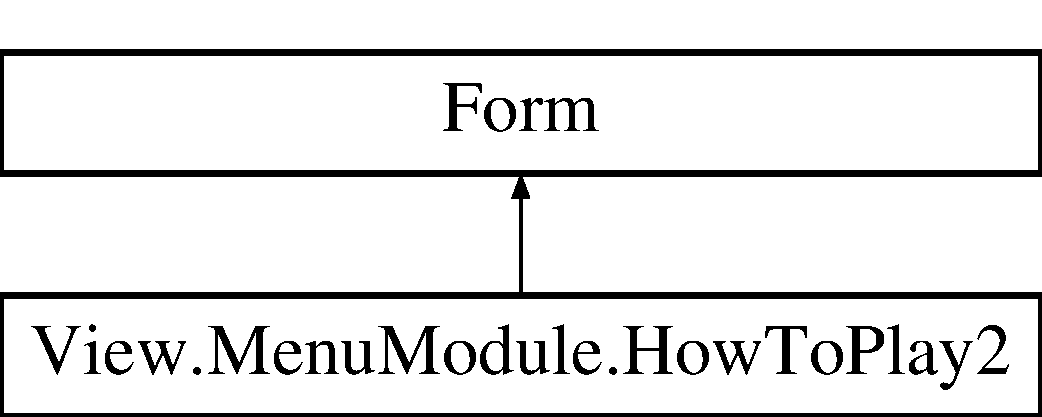
\includegraphics[height=2.000000cm]{class_view_1_1_menu_module_1_1_how_to_play2}
\end{center}
\end{figure}
\subsection*{Public Member Functions}
\begin{DoxyCompactItemize}
\item 
\hyperlink{class_view_1_1_menu_module_1_1_how_to_play2_ac0069718a15c08929de5228baef2b805}{How\+To\+Play2} ()
\item 
void \hyperlink{class_view_1_1_menu_module_1_1_how_to_play2_a937e82de93a8ab6842574109cfc48683}{set\+Quit\+False} ()
\item 
Boolean \hyperlink{class_view_1_1_menu_module_1_1_how_to_play2_af3cfed592dae438daa6edc729fb4893f}{get\+Quit} ()
\item 
void \hyperlink{class_view_1_1_menu_module_1_1_how_to_play2_a05ea9b0ee4a7be839332c4fb6f709b98}{set\+Next\+False} ()
\item 
Boolean \hyperlink{class_view_1_1_menu_module_1_1_how_to_play2_a87c3fef50b6780fbe2ed6d7798849504}{get\+Next} ()
\end{DoxyCompactItemize}
\subsection*{Public Attributes}
\begin{DoxyCompactItemize}
\item 
bool \hyperlink{class_view_1_1_menu_module_1_1_how_to_play2_af31369fd9237a7c96ede9eb79d749223}{quit} = false
\item 
bool \hyperlink{class_view_1_1_menu_module_1_1_how_to_play2_af60010a959740d9fe7089ed0e2a979bc}{next} = false
\end{DoxyCompactItemize}
\subsection*{Protected Member Functions}
\begin{DoxyCompactItemize}
\item 
override void \hyperlink{class_view_1_1_menu_module_1_1_how_to_play2_a697ecda1f98ad4557b3789a36a2c5a8e}{Dispose} (bool disposing)
\begin{DoxyCompactList}\small\item\em Clean up any resources being used. \end{DoxyCompactList}\end{DoxyCompactItemize}


\subsection{Detailed Description}
How to Play Menu 2 is opened with next is clicked on \hyperlink{class_view_1_1_menu_module_1_1_how_to_play}{How\+To\+Play} Menu 



\subsection{Constructor \& Destructor Documentation}
\hypertarget{class_view_1_1_menu_module_1_1_how_to_play2_ac0069718a15c08929de5228baef2b805}{}\label{class_view_1_1_menu_module_1_1_how_to_play2_ac0069718a15c08929de5228baef2b805} 
\index{View\+::\+Menu\+Module\+::\+How\+To\+Play2@{View\+::\+Menu\+Module\+::\+How\+To\+Play2}!How\+To\+Play2@{How\+To\+Play2}}
\index{How\+To\+Play2@{How\+To\+Play2}!View\+::\+Menu\+Module\+::\+How\+To\+Play2@{View\+::\+Menu\+Module\+::\+How\+To\+Play2}}
\subsubsection{\texorpdfstring{How\+To\+Play2()}{HowToPlay2()}}
{\footnotesize\ttfamily View.\+Menu\+Module.\+How\+To\+Play2.\+How\+To\+Play2 (\begin{DoxyParamCaption}{ }\end{DoxyParamCaption})\hspace{0.3cm}{\ttfamily [inline]}}

Constructor for \hyperlink{class_view_1_1_menu_module_1_1_how_to_play2}{How\+To\+Play2} window 

\subsection{Member Function Documentation}
\hypertarget{class_view_1_1_menu_module_1_1_how_to_play2_a697ecda1f98ad4557b3789a36a2c5a8e}{}\label{class_view_1_1_menu_module_1_1_how_to_play2_a697ecda1f98ad4557b3789a36a2c5a8e} 
\index{View\+::\+Menu\+Module\+::\+How\+To\+Play2@{View\+::\+Menu\+Module\+::\+How\+To\+Play2}!Dispose@{Dispose}}
\index{Dispose@{Dispose}!View\+::\+Menu\+Module\+::\+How\+To\+Play2@{View\+::\+Menu\+Module\+::\+How\+To\+Play2}}
\subsubsection{\texorpdfstring{Dispose()}{Dispose()}}
{\footnotesize\ttfamily override void View.\+Menu\+Module.\+How\+To\+Play2.\+Dispose (\begin{DoxyParamCaption}\item[{bool}]{disposing }\end{DoxyParamCaption})\hspace{0.3cm}{\ttfamily [inline]}, {\ttfamily [protected]}}



Clean up any resources being used. 


\begin{DoxyParams}{Parameters}
{\em disposing} & true if managed resources should be disposed; otherwise, false.\\
\hline
\end{DoxyParams}
\hypertarget{class_view_1_1_menu_module_1_1_how_to_play2_a87c3fef50b6780fbe2ed6d7798849504}{}\label{class_view_1_1_menu_module_1_1_how_to_play2_a87c3fef50b6780fbe2ed6d7798849504} 
\index{View\+::\+Menu\+Module\+::\+How\+To\+Play2@{View\+::\+Menu\+Module\+::\+How\+To\+Play2}!get\+Next@{get\+Next}}
\index{get\+Next@{get\+Next}!View\+::\+Menu\+Module\+::\+How\+To\+Play2@{View\+::\+Menu\+Module\+::\+How\+To\+Play2}}
\subsubsection{\texorpdfstring{get\+Next()}{getNext()}}
{\footnotesize\ttfamily Boolean View.\+Menu\+Module.\+How\+To\+Play2.\+get\+Next (\begin{DoxyParamCaption}{ }\end{DoxyParamCaption})\hspace{0.3cm}{\ttfamily [inline]}}

returns if quit button is currently clicked \hypertarget{class_view_1_1_menu_module_1_1_how_to_play2_af3cfed592dae438daa6edc729fb4893f}{}\label{class_view_1_1_menu_module_1_1_how_to_play2_af3cfed592dae438daa6edc729fb4893f} 
\index{View\+::\+Menu\+Module\+::\+How\+To\+Play2@{View\+::\+Menu\+Module\+::\+How\+To\+Play2}!get\+Quit@{get\+Quit}}
\index{get\+Quit@{get\+Quit}!View\+::\+Menu\+Module\+::\+How\+To\+Play2@{View\+::\+Menu\+Module\+::\+How\+To\+Play2}}
\subsubsection{\texorpdfstring{get\+Quit()}{getQuit()}}
{\footnotesize\ttfamily Boolean View.\+Menu\+Module.\+How\+To\+Play2.\+get\+Quit (\begin{DoxyParamCaption}{ }\end{DoxyParamCaption})\hspace{0.3cm}{\ttfamily [inline]}}

returns if quit button is currently clicked \hypertarget{class_view_1_1_menu_module_1_1_how_to_play2_a05ea9b0ee4a7be839332c4fb6f709b98}{}\label{class_view_1_1_menu_module_1_1_how_to_play2_a05ea9b0ee4a7be839332c4fb6f709b98} 
\index{View\+::\+Menu\+Module\+::\+How\+To\+Play2@{View\+::\+Menu\+Module\+::\+How\+To\+Play2}!set\+Next\+False@{set\+Next\+False}}
\index{set\+Next\+False@{set\+Next\+False}!View\+::\+Menu\+Module\+::\+How\+To\+Play2@{View\+::\+Menu\+Module\+::\+How\+To\+Play2}}
\subsubsection{\texorpdfstring{set\+Next\+False()}{setNextFalse()}}
{\footnotesize\ttfamily void View.\+Menu\+Module.\+How\+To\+Play2.\+set\+Next\+False (\begin{DoxyParamCaption}{ }\end{DoxyParamCaption})\hspace{0.3cm}{\ttfamily [inline]}}

checks if Game State is no longer inside How To Play \hypertarget{class_view_1_1_menu_module_1_1_how_to_play2_a937e82de93a8ab6842574109cfc48683}{}\label{class_view_1_1_menu_module_1_1_how_to_play2_a937e82de93a8ab6842574109cfc48683} 
\index{View\+::\+Menu\+Module\+::\+How\+To\+Play2@{View\+::\+Menu\+Module\+::\+How\+To\+Play2}!set\+Quit\+False@{set\+Quit\+False}}
\index{set\+Quit\+False@{set\+Quit\+False}!View\+::\+Menu\+Module\+::\+How\+To\+Play2@{View\+::\+Menu\+Module\+::\+How\+To\+Play2}}
\subsubsection{\texorpdfstring{set\+Quit\+False()}{setQuitFalse()}}
{\footnotesize\ttfamily void View.\+Menu\+Module.\+How\+To\+Play2.\+set\+Quit\+False (\begin{DoxyParamCaption}{ }\end{DoxyParamCaption})\hspace{0.3cm}{\ttfamily [inline]}}

checks if Game State is no longer inside How To Play 

\subsection{Member Data Documentation}
\hypertarget{class_view_1_1_menu_module_1_1_how_to_play2_af60010a959740d9fe7089ed0e2a979bc}{}\label{class_view_1_1_menu_module_1_1_how_to_play2_af60010a959740d9fe7089ed0e2a979bc} 
\index{View\+::\+Menu\+Module\+::\+How\+To\+Play2@{View\+::\+Menu\+Module\+::\+How\+To\+Play2}!next@{next}}
\index{next@{next}!View\+::\+Menu\+Module\+::\+How\+To\+Play2@{View\+::\+Menu\+Module\+::\+How\+To\+Play2}}
\subsubsection{\texorpdfstring{next}{next}}
{\footnotesize\ttfamily bool View.\+Menu\+Module.\+How\+To\+Play2.\+next = false}

boolean that checks if next button is clicked \hypertarget{class_view_1_1_menu_module_1_1_how_to_play2_af31369fd9237a7c96ede9eb79d749223}{}\label{class_view_1_1_menu_module_1_1_how_to_play2_af31369fd9237a7c96ede9eb79d749223} 
\index{View\+::\+Menu\+Module\+::\+How\+To\+Play2@{View\+::\+Menu\+Module\+::\+How\+To\+Play2}!quit@{quit}}
\index{quit@{quit}!View\+::\+Menu\+Module\+::\+How\+To\+Play2@{View\+::\+Menu\+Module\+::\+How\+To\+Play2}}
\subsubsection{\texorpdfstring{quit}{quit}}
{\footnotesize\ttfamily bool View.\+Menu\+Module.\+How\+To\+Play2.\+quit = false}

boolean that checks if quit button is clicked 

The documentation for this class was generated from the following files\+:\begin{DoxyCompactItemize}
\item 
How\+To\+Play2.\+cs\item 
How\+To\+Play2.\+Designer.\+cs\end{DoxyCompactItemize}

\hypertarget{class_view_1_1_menu_module_1_1_how_to_play3}{}\section{View.\+Menu\+Module.\+How\+To\+Play3 Class Reference}
\label{class_view_1_1_menu_module_1_1_how_to_play3}\index{View.\+Menu\+Module.\+How\+To\+Play3@{View.\+Menu\+Module.\+How\+To\+Play3}}


How to Play Menu 3 is opened with next is clicked on \hyperlink{class_view_1_1_menu_module_1_1_how_to_play2}{How\+To\+Play2} Menu  


Inheritance diagram for View.\+Menu\+Module.\+How\+To\+Play3\+:\begin{figure}[H]
\begin{center}
\leavevmode
\includegraphics[height=2.000000cm]{class_view_1_1_menu_module_1_1_how_to_play3}
\end{center}
\end{figure}
\subsection*{Public Member Functions}
\begin{DoxyCompactItemize}
\item 
\hyperlink{class_view_1_1_menu_module_1_1_how_to_play3_ad513e8bee12c26650d728609e59b208d}{How\+To\+Play3} ()
\item 
void \hyperlink{class_view_1_1_menu_module_1_1_how_to_play3_a7fd292034475f8a0fcb57a401808d043}{set\+Quit\+False} ()
\item 
Boolean \hyperlink{class_view_1_1_menu_module_1_1_how_to_play3_a32b39a8045e75e8cae4c94677d1be020}{get\+Quit} ()
\end{DoxyCompactItemize}
\subsection*{Public Attributes}
\begin{DoxyCompactItemize}
\item 
bool \hyperlink{class_view_1_1_menu_module_1_1_how_to_play3_a67ceaf31171526b8fab29a36094e983d}{quit} = false
\end{DoxyCompactItemize}
\subsection*{Protected Member Functions}
\begin{DoxyCompactItemize}
\item 
override void \hyperlink{class_view_1_1_menu_module_1_1_how_to_play3_a8335930fd58168dbcc5eddc120829d60}{Dispose} (bool disposing)
\begin{DoxyCompactList}\small\item\em Clean up any resources being used. \end{DoxyCompactList}\end{DoxyCompactItemize}


\subsection{Detailed Description}
How to Play Menu 3 is opened with next is clicked on \hyperlink{class_view_1_1_menu_module_1_1_how_to_play2}{How\+To\+Play2} Menu 



\subsection{Constructor \& Destructor Documentation}
\hypertarget{class_view_1_1_menu_module_1_1_how_to_play3_ad513e8bee12c26650d728609e59b208d}{}\label{class_view_1_1_menu_module_1_1_how_to_play3_ad513e8bee12c26650d728609e59b208d} 
\index{View\+::\+Menu\+Module\+::\+How\+To\+Play3@{View\+::\+Menu\+Module\+::\+How\+To\+Play3}!How\+To\+Play3@{How\+To\+Play3}}
\index{How\+To\+Play3@{How\+To\+Play3}!View\+::\+Menu\+Module\+::\+How\+To\+Play3@{View\+::\+Menu\+Module\+::\+How\+To\+Play3}}
\subsubsection{\texorpdfstring{How\+To\+Play3()}{HowToPlay3()}}
{\footnotesize\ttfamily View.\+Menu\+Module.\+How\+To\+Play3.\+How\+To\+Play3 (\begin{DoxyParamCaption}{ }\end{DoxyParamCaption})\hspace{0.3cm}{\ttfamily [inline]}}

Constructor for \hyperlink{class_view_1_1_menu_module_1_1_how_to_play3}{How\+To\+Play3} window 

\subsection{Member Function Documentation}
\hypertarget{class_view_1_1_menu_module_1_1_how_to_play3_a8335930fd58168dbcc5eddc120829d60}{}\label{class_view_1_1_menu_module_1_1_how_to_play3_a8335930fd58168dbcc5eddc120829d60} 
\index{View\+::\+Menu\+Module\+::\+How\+To\+Play3@{View\+::\+Menu\+Module\+::\+How\+To\+Play3}!Dispose@{Dispose}}
\index{Dispose@{Dispose}!View\+::\+Menu\+Module\+::\+How\+To\+Play3@{View\+::\+Menu\+Module\+::\+How\+To\+Play3}}
\subsubsection{\texorpdfstring{Dispose()}{Dispose()}}
{\footnotesize\ttfamily override void View.\+Menu\+Module.\+How\+To\+Play3.\+Dispose (\begin{DoxyParamCaption}\item[{bool}]{disposing }\end{DoxyParamCaption})\hspace{0.3cm}{\ttfamily [inline]}, {\ttfamily [protected]}}



Clean up any resources being used. 


\begin{DoxyParams}{Parameters}
{\em disposing} & true if managed resources should be disposed; otherwise, false.\\
\hline
\end{DoxyParams}
\hypertarget{class_view_1_1_menu_module_1_1_how_to_play3_a32b39a8045e75e8cae4c94677d1be020}{}\label{class_view_1_1_menu_module_1_1_how_to_play3_a32b39a8045e75e8cae4c94677d1be020} 
\index{View\+::\+Menu\+Module\+::\+How\+To\+Play3@{View\+::\+Menu\+Module\+::\+How\+To\+Play3}!get\+Quit@{get\+Quit}}
\index{get\+Quit@{get\+Quit}!View\+::\+Menu\+Module\+::\+How\+To\+Play3@{View\+::\+Menu\+Module\+::\+How\+To\+Play3}}
\subsubsection{\texorpdfstring{get\+Quit()}{getQuit()}}
{\footnotesize\ttfamily Boolean View.\+Menu\+Module.\+How\+To\+Play3.\+get\+Quit (\begin{DoxyParamCaption}{ }\end{DoxyParamCaption})\hspace{0.3cm}{\ttfamily [inline]}}

returns if quit button is currently clicked \hypertarget{class_view_1_1_menu_module_1_1_how_to_play3_a7fd292034475f8a0fcb57a401808d043}{}\label{class_view_1_1_menu_module_1_1_how_to_play3_a7fd292034475f8a0fcb57a401808d043} 
\index{View\+::\+Menu\+Module\+::\+How\+To\+Play3@{View\+::\+Menu\+Module\+::\+How\+To\+Play3}!set\+Quit\+False@{set\+Quit\+False}}
\index{set\+Quit\+False@{set\+Quit\+False}!View\+::\+Menu\+Module\+::\+How\+To\+Play3@{View\+::\+Menu\+Module\+::\+How\+To\+Play3}}
\subsubsection{\texorpdfstring{set\+Quit\+False()}{setQuitFalse()}}
{\footnotesize\ttfamily void View.\+Menu\+Module.\+How\+To\+Play3.\+set\+Quit\+False (\begin{DoxyParamCaption}{ }\end{DoxyParamCaption})\hspace{0.3cm}{\ttfamily [inline]}}

checks if Game State is no longer inside How To Play 

\subsection{Member Data Documentation}
\hypertarget{class_view_1_1_menu_module_1_1_how_to_play3_a67ceaf31171526b8fab29a36094e983d}{}\label{class_view_1_1_menu_module_1_1_how_to_play3_a67ceaf31171526b8fab29a36094e983d} 
\index{View\+::\+Menu\+Module\+::\+How\+To\+Play3@{View\+::\+Menu\+Module\+::\+How\+To\+Play3}!quit@{quit}}
\index{quit@{quit}!View\+::\+Menu\+Module\+::\+How\+To\+Play3@{View\+::\+Menu\+Module\+::\+How\+To\+Play3}}
\subsubsection{\texorpdfstring{quit}{quit}}
{\footnotesize\ttfamily bool View.\+Menu\+Module.\+How\+To\+Play3.\+quit = false}

boolean that checks if quit button is clicked 

The documentation for this class was generated from the following files\+:\begin{DoxyCompactItemize}
\item 
How\+To\+Play3.\+cs\item 
How\+To\+Play3.\+Designer.\+cs\end{DoxyCompactItemize}

\hypertarget{class_model_1_1_weapon_module_1_1_iron_sword}{}\section{Model.\+Weapon\+Module.\+Iron\+Sword Class Reference}
\label{class_model_1_1_weapon_module_1_1_iron_sword}\index{Model.\+Weapon\+Module.\+Iron\+Sword@{Model.\+Weapon\+Module.\+Iron\+Sword}}


Melee Physical \hyperlink{interface_model_1_1_weapon_module_1_1_weapon}{Weapon}.  


Inheritance diagram for Model.\+Weapon\+Module.\+Iron\+Sword\+:\begin{figure}[H]
\begin{center}
\leavevmode
\includegraphics[height=2.000000cm]{class_model_1_1_weapon_module_1_1_iron_sword}
\end{center}
\end{figure}
\subsection*{Public Member Functions}
\begin{DoxyCompactItemize}
\item 
\hyperlink{class_model_1_1_weapon_module_1_1_iron_sword_ab4d225fec1f0784f801740c1a4b65a25}{Iron\+Sword} ()
\item 
\hyperlink{namespace_model_1_1_weapon_module_a3390c266f89e3399c2bc7fa31f13cbec}{weapon\+Type} \hyperlink{class_model_1_1_weapon_module_1_1_iron_sword_a886800dd0c3fbebebbf410dab9f91454}{get\+Weap\+Type} ()
\end{DoxyCompactItemize}
\subsection*{Properties}
\begin{DoxyCompactItemize}
\item 
int \hyperlink{class_model_1_1_weapon_module_1_1_iron_sword_ae2b8382a3b1cae70238fa408cf615aa7}{mod\+Str}\hspace{0.3cm}{\ttfamily  \mbox{[}get\mbox{]}}
\item 
int \hyperlink{class_model_1_1_weapon_module_1_1_iron_sword_ab0cfe8f4f6c606284d0e7c91b1696fc7}{mod\+Int}\hspace{0.3cm}{\ttfamily  \mbox{[}get\mbox{]}}
\item 
int \hyperlink{class_model_1_1_weapon_module_1_1_iron_sword_a81527447c2cdeda0e634bb7ac9c2bb90}{mod\+Skill}\hspace{0.3cm}{\ttfamily  \mbox{[}get\mbox{]}}
\item 
string \hyperlink{class_model_1_1_weapon_module_1_1_iron_sword_a57f5bf0fb116a9e6208e36dec42736b6}{name}\hspace{0.3cm}{\ttfamily  \mbox{[}get\mbox{]}}
\item 
int \mbox{[}$\,$\mbox{]} \hyperlink{class_model_1_1_weapon_module_1_1_iron_sword_a0d87a7bfe8e0e2350a18a79525e812d2}{range}\hspace{0.3cm}{\ttfamily  \mbox{[}get\mbox{]}}
\end{DoxyCompactItemize}


\subsection{Detailed Description}
Melee Physical \hyperlink{interface_model_1_1_weapon_module_1_1_weapon}{Weapon}. 

This class represents a melee weapon. It implements the \hyperlink{interface_model_1_1_weapon_module_1_1_weapon}{Weapon} interface. 

\subsection{Constructor \& Destructor Documentation}
\hypertarget{class_model_1_1_weapon_module_1_1_iron_sword_ab4d225fec1f0784f801740c1a4b65a25}{}\label{class_model_1_1_weapon_module_1_1_iron_sword_ab4d225fec1f0784f801740c1a4b65a25} 
\index{Model\+::\+Weapon\+Module\+::\+Iron\+Sword@{Model\+::\+Weapon\+Module\+::\+Iron\+Sword}!Iron\+Sword@{Iron\+Sword}}
\index{Iron\+Sword@{Iron\+Sword}!Model\+::\+Weapon\+Module\+::\+Iron\+Sword@{Model\+::\+Weapon\+Module\+::\+Iron\+Sword}}
\subsubsection{\texorpdfstring{Iron\+Sword()}{IronSword()}}
{\footnotesize\ttfamily Model.\+Weapon\+Module.\+Iron\+Sword.\+Iron\+Sword (\begin{DoxyParamCaption}{ }\end{DoxyParamCaption})\hspace{0.3cm}{\ttfamily [inline]}}

Constructs a Iron Sword weapon with stats\+: 7str, 3skill, 0int, and a range of 1 with name Iron Sword. 

\subsection{Member Function Documentation}
\hypertarget{class_model_1_1_weapon_module_1_1_iron_sword_a886800dd0c3fbebebbf410dab9f91454}{}\label{class_model_1_1_weapon_module_1_1_iron_sword_a886800dd0c3fbebebbf410dab9f91454} 
\index{Model\+::\+Weapon\+Module\+::\+Iron\+Sword@{Model\+::\+Weapon\+Module\+::\+Iron\+Sword}!get\+Weap\+Type@{get\+Weap\+Type}}
\index{get\+Weap\+Type@{get\+Weap\+Type}!Model\+::\+Weapon\+Module\+::\+Iron\+Sword@{Model\+::\+Weapon\+Module\+::\+Iron\+Sword}}
\subsubsection{\texorpdfstring{get\+Weap\+Type()}{getWeapType()}}
{\footnotesize\ttfamily \hyperlink{namespace_model_1_1_weapon_module_a3390c266f89e3399c2bc7fa31f13cbec}{weapon\+Type} Model.\+Weapon\+Module.\+Iron\+Sword.\+get\+Weap\+Type (\begin{DoxyParamCaption}{ }\end{DoxyParamCaption})\hspace{0.3cm}{\ttfamily [inline]}}

Returns the weapon type. 

Implements \hyperlink{interface_model_1_1_weapon_module_1_1_weapon_a175133855ef446d3d87c70d13979be9c}{Model.\+Weapon\+Module.\+Weapon}.



\subsection{Property Documentation}
\hypertarget{class_model_1_1_weapon_module_1_1_iron_sword_ab0cfe8f4f6c606284d0e7c91b1696fc7}{}\label{class_model_1_1_weapon_module_1_1_iron_sword_ab0cfe8f4f6c606284d0e7c91b1696fc7} 
\index{Model\+::\+Weapon\+Module\+::\+Iron\+Sword@{Model\+::\+Weapon\+Module\+::\+Iron\+Sword}!mod\+Int@{mod\+Int}}
\index{mod\+Int@{mod\+Int}!Model\+::\+Weapon\+Module\+::\+Iron\+Sword@{Model\+::\+Weapon\+Module\+::\+Iron\+Sword}}
\subsubsection{\texorpdfstring{mod\+Int}{modInt}}
{\footnotesize\ttfamily int Model.\+Weapon\+Module.\+Iron\+Sword.\+mod\+Int\hspace{0.3cm}{\ttfamily [get]}}

Returns the weapon intelligence. \hypertarget{class_model_1_1_weapon_module_1_1_iron_sword_a81527447c2cdeda0e634bb7ac9c2bb90}{}\label{class_model_1_1_weapon_module_1_1_iron_sword_a81527447c2cdeda0e634bb7ac9c2bb90} 
\index{Model\+::\+Weapon\+Module\+::\+Iron\+Sword@{Model\+::\+Weapon\+Module\+::\+Iron\+Sword}!mod\+Skill@{mod\+Skill}}
\index{mod\+Skill@{mod\+Skill}!Model\+::\+Weapon\+Module\+::\+Iron\+Sword@{Model\+::\+Weapon\+Module\+::\+Iron\+Sword}}
\subsubsection{\texorpdfstring{mod\+Skill}{modSkill}}
{\footnotesize\ttfamily int Model.\+Weapon\+Module.\+Iron\+Sword.\+mod\+Skill\hspace{0.3cm}{\ttfamily [get]}}

Returns the weapon skill. \hypertarget{class_model_1_1_weapon_module_1_1_iron_sword_ae2b8382a3b1cae70238fa408cf615aa7}{}\label{class_model_1_1_weapon_module_1_1_iron_sword_ae2b8382a3b1cae70238fa408cf615aa7} 
\index{Model\+::\+Weapon\+Module\+::\+Iron\+Sword@{Model\+::\+Weapon\+Module\+::\+Iron\+Sword}!mod\+Str@{mod\+Str}}
\index{mod\+Str@{mod\+Str}!Model\+::\+Weapon\+Module\+::\+Iron\+Sword@{Model\+::\+Weapon\+Module\+::\+Iron\+Sword}}
\subsubsection{\texorpdfstring{mod\+Str}{modStr}}
{\footnotesize\ttfamily int Model.\+Weapon\+Module.\+Iron\+Sword.\+mod\+Str\hspace{0.3cm}{\ttfamily [get]}}

Returns the weapon strength. \hypertarget{class_model_1_1_weapon_module_1_1_iron_sword_a57f5bf0fb116a9e6208e36dec42736b6}{}\label{class_model_1_1_weapon_module_1_1_iron_sword_a57f5bf0fb116a9e6208e36dec42736b6} 
\index{Model\+::\+Weapon\+Module\+::\+Iron\+Sword@{Model\+::\+Weapon\+Module\+::\+Iron\+Sword}!name@{name}}
\index{name@{name}!Model\+::\+Weapon\+Module\+::\+Iron\+Sword@{Model\+::\+Weapon\+Module\+::\+Iron\+Sword}}
\subsubsection{\texorpdfstring{name}{name}}
{\footnotesize\ttfamily string Model.\+Weapon\+Module.\+Iron\+Sword.\+name\hspace{0.3cm}{\ttfamily [get]}}

Returns the name of the weapon. \hypertarget{class_model_1_1_weapon_module_1_1_iron_sword_a0d87a7bfe8e0e2350a18a79525e812d2}{}\label{class_model_1_1_weapon_module_1_1_iron_sword_a0d87a7bfe8e0e2350a18a79525e812d2} 
\index{Model\+::\+Weapon\+Module\+::\+Iron\+Sword@{Model\+::\+Weapon\+Module\+::\+Iron\+Sword}!range@{range}}
\index{range@{range}!Model\+::\+Weapon\+Module\+::\+Iron\+Sword@{Model\+::\+Weapon\+Module\+::\+Iron\+Sword}}
\subsubsection{\texorpdfstring{range}{range}}
{\footnotesize\ttfamily int \mbox{[}$\,$\mbox{]} Model.\+Weapon\+Module.\+Iron\+Sword.\+range\hspace{0.3cm}{\ttfamily [get]}}

Return the range of the weapon, where range\mbox{[}minimum range, maximum range\mbox{]}. 

The documentation for this class was generated from the following file\+:\begin{DoxyCompactItemize}
\item 
Iron\+Sword.\+cs\end{DoxyCompactItemize}

\hypertarget{class_model_1_1_weapon_module_1_1_long_bow}{}\section{Model.\+Weapon\+Module.\+Long\+Bow Class Reference}
\label{class_model_1_1_weapon_module_1_1_long_bow}\index{Model.\+Weapon\+Module.\+Long\+Bow@{Model.\+Weapon\+Module.\+Long\+Bow}}


Ranged physical \hyperlink{interface_model_1_1_weapon_module_1_1_weapon}{Weapon}.  


Inheritance diagram for Model.\+Weapon\+Module.\+Long\+Bow\+:\begin{figure}[H]
\begin{center}
\leavevmode
\includegraphics[height=2.000000cm]{class_model_1_1_weapon_module_1_1_long_bow}
\end{center}
\end{figure}
\subsection*{Public Member Functions}
\begin{DoxyCompactItemize}
\item 
\hyperlink{class_model_1_1_weapon_module_1_1_long_bow_adbd4822fe9ff1519a2c226f0a1e8ee85}{Long\+Bow} ()
\item 
\hyperlink{namespace_model_1_1_weapon_module_a3390c266f89e3399c2bc7fa31f13cbec}{weapon\+Type} \hyperlink{class_model_1_1_weapon_module_1_1_long_bow_aca2986d43dcefb1f3d99c6507a4390cd}{get\+Weap\+Type} ()
\end{DoxyCompactItemize}
\subsection*{Properties}
\begin{DoxyCompactItemize}
\item 
int \hyperlink{class_model_1_1_weapon_module_1_1_long_bow_aefa38571f2e824c436833b8fed1b8e65}{mod\+Str}\hspace{0.3cm}{\ttfamily  \mbox{[}get\mbox{]}}
\item 
int \hyperlink{class_model_1_1_weapon_module_1_1_long_bow_a0a9b8b342ba911bc9d39ea5c388a9241}{mod\+Int}\hspace{0.3cm}{\ttfamily  \mbox{[}get\mbox{]}}
\item 
int \hyperlink{class_model_1_1_weapon_module_1_1_long_bow_a11e8c0740b84af41799a81faf98410b3}{mod\+Skill}\hspace{0.3cm}{\ttfamily  \mbox{[}get\mbox{]}}
\item 
string \hyperlink{class_model_1_1_weapon_module_1_1_long_bow_a74c5ca976caf85a52e651746e53c9b62}{name}\hspace{0.3cm}{\ttfamily  \mbox{[}get\mbox{]}}
\item 
int \mbox{[}$\,$\mbox{]} \hyperlink{class_model_1_1_weapon_module_1_1_long_bow_ad1c1cd55b24378a0496c669d66cfc459}{range}\hspace{0.3cm}{\ttfamily  \mbox{[}get\mbox{]}}
\end{DoxyCompactItemize}


\subsection{Detailed Description}
Ranged physical \hyperlink{interface_model_1_1_weapon_module_1_1_weapon}{Weapon}. 

This class represents a ranged weapon. It implements the \hyperlink{interface_model_1_1_weapon_module_1_1_weapon}{Weapon} interface. 

\subsection{Constructor \& Destructor Documentation}
\hypertarget{class_model_1_1_weapon_module_1_1_long_bow_adbd4822fe9ff1519a2c226f0a1e8ee85}{}\label{class_model_1_1_weapon_module_1_1_long_bow_adbd4822fe9ff1519a2c226f0a1e8ee85} 
\index{Model\+::\+Weapon\+Module\+::\+Long\+Bow@{Model\+::\+Weapon\+Module\+::\+Long\+Bow}!Long\+Bow@{Long\+Bow}}
\index{Long\+Bow@{Long\+Bow}!Model\+::\+Weapon\+Module\+::\+Long\+Bow@{Model\+::\+Weapon\+Module\+::\+Long\+Bow}}
\subsubsection{\texorpdfstring{Long\+Bow()}{LongBow()}}
{\footnotesize\ttfamily Model.\+Weapon\+Module.\+Long\+Bow.\+Long\+Bow (\begin{DoxyParamCaption}{ }\end{DoxyParamCaption})\hspace{0.3cm}{\ttfamily [inline]}}

Constructs a \hyperlink{class_model_1_1_weapon_module_1_1_long_bow}{Long\+Bow} weapon with stats\+: 7str, 8skill, 0int, and a range of 2-\/3 with name Long Bows 

\subsection{Member Function Documentation}
\hypertarget{class_model_1_1_weapon_module_1_1_long_bow_aca2986d43dcefb1f3d99c6507a4390cd}{}\label{class_model_1_1_weapon_module_1_1_long_bow_aca2986d43dcefb1f3d99c6507a4390cd} 
\index{Model\+::\+Weapon\+Module\+::\+Long\+Bow@{Model\+::\+Weapon\+Module\+::\+Long\+Bow}!get\+Weap\+Type@{get\+Weap\+Type}}
\index{get\+Weap\+Type@{get\+Weap\+Type}!Model\+::\+Weapon\+Module\+::\+Long\+Bow@{Model\+::\+Weapon\+Module\+::\+Long\+Bow}}
\subsubsection{\texorpdfstring{get\+Weap\+Type()}{getWeapType()}}
{\footnotesize\ttfamily \hyperlink{namespace_model_1_1_weapon_module_a3390c266f89e3399c2bc7fa31f13cbec}{weapon\+Type} Model.\+Weapon\+Module.\+Long\+Bow.\+get\+Weap\+Type (\begin{DoxyParamCaption}{ }\end{DoxyParamCaption})\hspace{0.3cm}{\ttfamily [inline]}}

Returns the weapon type. 

Implements \hyperlink{interface_model_1_1_weapon_module_1_1_weapon_a175133855ef446d3d87c70d13979be9c}{Model.\+Weapon\+Module.\+Weapon}.



\subsection{Property Documentation}
\hypertarget{class_model_1_1_weapon_module_1_1_long_bow_a0a9b8b342ba911bc9d39ea5c388a9241}{}\label{class_model_1_1_weapon_module_1_1_long_bow_a0a9b8b342ba911bc9d39ea5c388a9241} 
\index{Model\+::\+Weapon\+Module\+::\+Long\+Bow@{Model\+::\+Weapon\+Module\+::\+Long\+Bow}!mod\+Int@{mod\+Int}}
\index{mod\+Int@{mod\+Int}!Model\+::\+Weapon\+Module\+::\+Long\+Bow@{Model\+::\+Weapon\+Module\+::\+Long\+Bow}}
\subsubsection{\texorpdfstring{mod\+Int}{modInt}}
{\footnotesize\ttfamily int Model.\+Weapon\+Module.\+Long\+Bow.\+mod\+Int\hspace{0.3cm}{\ttfamily [get]}}

Returns the weapon intelligence. \hypertarget{class_model_1_1_weapon_module_1_1_long_bow_a11e8c0740b84af41799a81faf98410b3}{}\label{class_model_1_1_weapon_module_1_1_long_bow_a11e8c0740b84af41799a81faf98410b3} 
\index{Model\+::\+Weapon\+Module\+::\+Long\+Bow@{Model\+::\+Weapon\+Module\+::\+Long\+Bow}!mod\+Skill@{mod\+Skill}}
\index{mod\+Skill@{mod\+Skill}!Model\+::\+Weapon\+Module\+::\+Long\+Bow@{Model\+::\+Weapon\+Module\+::\+Long\+Bow}}
\subsubsection{\texorpdfstring{mod\+Skill}{modSkill}}
{\footnotesize\ttfamily int Model.\+Weapon\+Module.\+Long\+Bow.\+mod\+Skill\hspace{0.3cm}{\ttfamily [get]}}

Returns the weapon skill. \hypertarget{class_model_1_1_weapon_module_1_1_long_bow_aefa38571f2e824c436833b8fed1b8e65}{}\label{class_model_1_1_weapon_module_1_1_long_bow_aefa38571f2e824c436833b8fed1b8e65} 
\index{Model\+::\+Weapon\+Module\+::\+Long\+Bow@{Model\+::\+Weapon\+Module\+::\+Long\+Bow}!mod\+Str@{mod\+Str}}
\index{mod\+Str@{mod\+Str}!Model\+::\+Weapon\+Module\+::\+Long\+Bow@{Model\+::\+Weapon\+Module\+::\+Long\+Bow}}
\subsubsection{\texorpdfstring{mod\+Str}{modStr}}
{\footnotesize\ttfamily int Model.\+Weapon\+Module.\+Long\+Bow.\+mod\+Str\hspace{0.3cm}{\ttfamily [get]}}

Returns the weapon strength. \hypertarget{class_model_1_1_weapon_module_1_1_long_bow_a74c5ca976caf85a52e651746e53c9b62}{}\label{class_model_1_1_weapon_module_1_1_long_bow_a74c5ca976caf85a52e651746e53c9b62} 
\index{Model\+::\+Weapon\+Module\+::\+Long\+Bow@{Model\+::\+Weapon\+Module\+::\+Long\+Bow}!name@{name}}
\index{name@{name}!Model\+::\+Weapon\+Module\+::\+Long\+Bow@{Model\+::\+Weapon\+Module\+::\+Long\+Bow}}
\subsubsection{\texorpdfstring{name}{name}}
{\footnotesize\ttfamily string Model.\+Weapon\+Module.\+Long\+Bow.\+name\hspace{0.3cm}{\ttfamily [get]}}

Returns the name of the weapon. \hypertarget{class_model_1_1_weapon_module_1_1_long_bow_ad1c1cd55b24378a0496c669d66cfc459}{}\label{class_model_1_1_weapon_module_1_1_long_bow_ad1c1cd55b24378a0496c669d66cfc459} 
\index{Model\+::\+Weapon\+Module\+::\+Long\+Bow@{Model\+::\+Weapon\+Module\+::\+Long\+Bow}!range@{range}}
\index{range@{range}!Model\+::\+Weapon\+Module\+::\+Long\+Bow@{Model\+::\+Weapon\+Module\+::\+Long\+Bow}}
\subsubsection{\texorpdfstring{range}{range}}
{\footnotesize\ttfamily int \mbox{[}$\,$\mbox{]} Model.\+Weapon\+Module.\+Long\+Bow.\+range\hspace{0.3cm}{\ttfamily [get]}}

Return the range of the weapon, where range\mbox{[}minimum range, maximum range\mbox{]}. 

The documentation for this class was generated from the following file\+:\begin{DoxyCompactItemize}
\item 
Long\+Bow.\+cs\end{DoxyCompactItemize}

\hypertarget{class_model_1_1_unit_module_1_1_mage}{}\section{Model.\+Unit\+Module.\+Mage Class Reference}
\label{class_model_1_1_unit_module_1_1_mage}\index{Model.\+Unit\+Module.\+Mage@{Model.\+Unit\+Module.\+Mage}}


The \hyperlink{class_model_1_1_unit_module_1_1_mage}{Mage} model class, extends \hyperlink{interface_model_1_1_unit_module_1_1_unit}{Unit}. ~\newline
 This \hyperlink{interface_model_1_1_unit_module_1_1_unit}{Unit} has strong magical capabilities, and is capable of powerful ranged magic attacks, but makes up with poor physical stats.  


Inheritance diagram for Model.\+Unit\+Module.\+Mage\+:\begin{figure}[H]
\begin{center}
\leavevmode
\includegraphics[height=2.000000cm]{class_model_1_1_unit_module_1_1_mage}
\end{center}
\end{figure}
\subsection*{Public Member Functions}
\begin{DoxyCompactItemize}
\item 
\hyperlink{class_model_1_1_unit_module_1_1_mage_a7ffb443153df0abdc04ceb1da6f1b241}{Mage} (Texture2D sprite\+Image, \hyperlink{class_model_1_1_button}{Button}\mbox{[}$\,$\mbox{]} unit\+Buttons, Texture2D char\+Info, Texture2D char\+Attack\+Info, Vector2 coordinates, Texture2D health\+Bar)
\item 
void \hyperlink{class_model_1_1_unit_module_1_1_mage_a7b16a0324edbd7daa0d54ba5b6bd9735}{set\+Initial\+Stats} ()
\item 
int \hyperlink{class_model_1_1_unit_module_1_1_mage_a85e20ef350f937c14e6de3362c0cdcfb}{get\+Movability} ()
\item 
int \mbox{[}$\,$\mbox{]} \hyperlink{class_model_1_1_unit_module_1_1_mage_aa7cb642ad7aadd1161f1d95e501dfd23}{get\+Stats} ()
\item 
\hyperlink{interface_model_1_1_weapon_module_1_1_weapon}{Weapon} \mbox{[}$\,$\mbox{]} \hyperlink{class_model_1_1_unit_module_1_1_mage_a97144d7360321515956ebb92e8bd0caf}{get\+Equipable\+Weapons} ()
\item 
\hyperlink{namespace_model_1_1_unit_module_aba9769f408747bf38d0d8adca8f68c98}{Unit\+Type} \hyperlink{class_model_1_1_unit_module_1_1_mage_a1fa4709e8927042bfd858a330d8cba22}{get\+Class} ()
\item 
Texture2D \hyperlink{class_model_1_1_unit_module_1_1_mage_a1b771ad25cbaf34997af030b867a5131}{get\+Sprite\+Image} ()
\item 
Texture2D \hyperlink{class_model_1_1_unit_module_1_1_mage_ac15d8706f49bcd67b7492e4e91eff15b}{get\+Button\+Image} (\hyperlink{namespace_model_ac76b3489c9d704f49912608bd36cd0e7}{Button\+Type} button\+Type)
\item 
bool \hyperlink{class_model_1_1_unit_module_1_1_mage_a7a6f09d97b1065dfadd2b7722b80045d}{is\+Button\+Active} (\hyperlink{namespace_model_ac76b3489c9d704f49912608bd36cd0e7}{Button\+Type} button\+Type)
\item 
Texture2D \hyperlink{class_model_1_1_unit_module_1_1_mage_a6c9b2e9f98ed461b77559c1241407c94}{get\+Char\+Info} ()
\item 
Texture2D \hyperlink{class_model_1_1_unit_module_1_1_mage_a69d22e6d54e3f0d7f3cf8b1029755ffe}{get\+Char\+Attack\+Info} ()
\item 
\hyperlink{class_model_1_1_button}{Button} \mbox{[}$\,$\mbox{]} \hyperlink{class_model_1_1_unit_module_1_1_mage_a830affe9a902833c691f89d103b50d31}{get\+Buttons} ()
\item 
\hyperlink{class_model_1_1_button}{Button} \hyperlink{class_model_1_1_unit_module_1_1_mage_a996253aeeb97c7a5d64ad81c03adf0f0}{get\+Button\+Type} (\hyperlink{namespace_model_ac76b3489c9d704f49912608bd36cd0e7}{Button\+Type} button\+Type)
\item 
void \hyperlink{class_model_1_1_unit_module_1_1_mage_a2cbdb537e8039e19367b2d9905847e1b}{set\+Button\+Coordinates} (Vector2 pixel\+Coordinates)
\item 
Rectangle \hyperlink{class_model_1_1_unit_module_1_1_mage_a66ef058e38d7220bc65604504eb25bce}{get\+Current\+Frame} ()
\item 
Texture2D \hyperlink{class_model_1_1_unit_module_1_1_mage_af816450e9803b56a1bf97bb9f04c2008}{get\+Health\+Bar} ()
\item 
int \hyperlink{class_model_1_1_unit_module_1_1_mage_a3b3a869faa3d4014175b79c87d18c865}{get\+Max\+Hp} ()
\end{DoxyCompactItemize}
\subsection*{Properties}
\begin{DoxyCompactItemize}
\item 
bool \hyperlink{class_model_1_1_unit_module_1_1_mage_aedac42cbab6a6e18fef3237f9996552b}{Alive}\hspace{0.3cm}{\ttfamily  \mbox{[}get, set\mbox{]}}
\item 
int \hyperlink{class_model_1_1_unit_module_1_1_mage_af6c66da17b184fbe0fd15ca059cadde3}{Speed}\hspace{0.3cm}{\ttfamily  \mbox{[}get, set\mbox{]}}
\item 
int \hyperlink{class_model_1_1_unit_module_1_1_mage_ab656a61ced3728b765d4239969484422}{Def}\hspace{0.3cm}{\ttfamily  \mbox{[}get, set\mbox{]}}
\item 
int \hyperlink{class_model_1_1_unit_module_1_1_mage_aaf72ba998d643cbb52930d00a44068bb}{Res}\hspace{0.3cm}{\ttfamily  \mbox{[}get, set\mbox{]}}
\item 
int \hyperlink{class_model_1_1_unit_module_1_1_mage_a3ee8585a9a8ef0f49de9e56638c6651e}{Level}\hspace{0.3cm}{\ttfamily  \mbox{[}get, set\mbox{]}}
\item 
\hyperlink{interface_model_1_1_weapon_module_1_1_weapon}{Weapon} \hyperlink{class_model_1_1_unit_module_1_1_mage_abf1f6f69bfaea68af1cee7f5a159221a}{equipped\+Weapon}\hspace{0.3cm}{\ttfamily  \mbox{[}get, set\mbox{]}}
\item 
int \hyperlink{class_model_1_1_unit_module_1_1_mage_a5d6361a991dc1726f5de85d2e2e31afd}{current\+Frame}\hspace{0.3cm}{\ttfamily  \mbox{[}get, set\mbox{]}}
\item 
int \hyperlink{class_model_1_1_unit_module_1_1_mage_a20fd3a8868f4c19b8b3e0373c1133446}{Str}\hspace{0.3cm}{\ttfamily  \mbox{[}get, set\mbox{]}}
\item 
int \hyperlink{class_model_1_1_unit_module_1_1_mage_aff8f2ffa9c6e416278d2ef5a4a39e7ba}{Int}\hspace{0.3cm}{\ttfamily  \mbox{[}get, set\mbox{]}}
\item 
int \hyperlink{class_model_1_1_unit_module_1_1_mage_af61303ab529c005f4fed6707672a905e}{Skill}\hspace{0.3cm}{\ttfamily  \mbox{[}get, set\mbox{]}}
\item 
int \hyperlink{class_model_1_1_unit_module_1_1_mage_a6a68c5f76a92eb24bb171f740a99e681}{Hp}\hspace{0.3cm}{\ttfamily  \mbox{[}get, set\mbox{]}}
\item 
Tuple$<$ int, int $>$ \hyperlink{class_model_1_1_unit_module_1_1_mage_a53b0e4a5a23887d56d2b359f676dafa7}{Position}\hspace{0.3cm}{\ttfamily  \mbox{[}get, set\mbox{]}}
\item 
Vector2 \hyperlink{class_model_1_1_unit_module_1_1_mage_ae115e4497d06b8938ceee7344dd1350d}{Pixel\+Coordinates}\hspace{0.3cm}{\ttfamily  \mbox{[}get, set\mbox{]}}
\end{DoxyCompactItemize}


\subsection{Detailed Description}
The \hyperlink{class_model_1_1_unit_module_1_1_mage}{Mage} model class, extends \hyperlink{interface_model_1_1_unit_module_1_1_unit}{Unit}. ~\newline
 This \hyperlink{interface_model_1_1_unit_module_1_1_unit}{Unit} has strong magical capabilities, and is capable of powerful ranged magic attacks, but makes up with poor physical stats. 



\subsection{Constructor \& Destructor Documentation}
\hypertarget{class_model_1_1_unit_module_1_1_mage_a7ffb443153df0abdc04ceb1da6f1b241}{}\label{class_model_1_1_unit_module_1_1_mage_a7ffb443153df0abdc04ceb1da6f1b241} 
\index{Model\+::\+Unit\+Module\+::\+Mage@{Model\+::\+Unit\+Module\+::\+Mage}!Mage@{Mage}}
\index{Mage@{Mage}!Model\+::\+Unit\+Module\+::\+Mage@{Model\+::\+Unit\+Module\+::\+Mage}}
\subsubsection{\texorpdfstring{Mage()}{Mage()}}
{\footnotesize\ttfamily Model.\+Unit\+Module.\+Mage.\+Mage (\begin{DoxyParamCaption}\item[{Texture2D}]{sprite\+Image,  }\item[{\hyperlink{class_model_1_1_button}{Button} \mbox{[}$\,$\mbox{]}}]{unit\+Buttons,  }\item[{Texture2D}]{char\+Info,  }\item[{Texture2D}]{char\+Attack\+Info,  }\item[{Vector2}]{coordinates,  }\item[{Texture2D}]{health\+Bar }\end{DoxyParamCaption})\hspace{0.3cm}{\ttfamily [inline]}}

The constructor for \hyperlink{interface_model_1_1_unit_module_1_1_unit}{Unit} \hyperlink{class_model_1_1_unit_module_1_1_mage}{Mage}. Stores all relevent data in model. 
\begin{DoxyParams}{Parameters}
{\em sprite\+Image} & The character sprite texture. \\
\hline
{\em unit\+Buttons} & The Texture2D Array containing all the different textures for each button. \\
\hline
{\em char\+Info} & The character info popup texture. \\
\hline
{\em char\+Attack\+Info} & The character attack menu popup texture. \\
\hline
{\em coordinates} & The unit\textquotesingle{}s current vector coordinate on screen. \\
\hline
{\em player} & The player of which the unit belongs to. \\
\hline
\end{DoxyParams}


\subsection{Member Function Documentation}
\hypertarget{class_model_1_1_unit_module_1_1_mage_ac15d8706f49bcd67b7492e4e91eff15b}{}\label{class_model_1_1_unit_module_1_1_mage_ac15d8706f49bcd67b7492e4e91eff15b} 
\index{Model\+::\+Unit\+Module\+::\+Mage@{Model\+::\+Unit\+Module\+::\+Mage}!get\+Button\+Image@{get\+Button\+Image}}
\index{get\+Button\+Image@{get\+Button\+Image}!Model\+::\+Unit\+Module\+::\+Mage@{Model\+::\+Unit\+Module\+::\+Mage}}
\subsubsection{\texorpdfstring{get\+Button\+Image()}{getButtonImage()}}
{\footnotesize\ttfamily Texture2D Model.\+Unit\+Module.\+Mage.\+get\+Button\+Image (\begin{DoxyParamCaption}\item[{\hyperlink{namespace_model_ac76b3489c9d704f49912608bd36cd0e7}{Button\+Type}}]{button\+Type }\end{DoxyParamCaption})\hspace{0.3cm}{\ttfamily [inline]}}

This method returns the texture associated with the buntton\+Type passed in, by going through a switch case and matching it. 
\begin{DoxyParams}{Parameters}
{\em button\+Type} & The buttontype that was clicked. \\
\hline
\end{DoxyParams}


Implements \hyperlink{interface_model_1_1_unit_module_1_1_unit_ac8e47a3f8d13fe8a719f962a3ee9ee46}{Model.\+Unit\+Module.\+Unit}.

\hypertarget{class_model_1_1_unit_module_1_1_mage_a830affe9a902833c691f89d103b50d31}{}\label{class_model_1_1_unit_module_1_1_mage_a830affe9a902833c691f89d103b50d31} 
\index{Model\+::\+Unit\+Module\+::\+Mage@{Model\+::\+Unit\+Module\+::\+Mage}!get\+Buttons@{get\+Buttons}}
\index{get\+Buttons@{get\+Buttons}!Model\+::\+Unit\+Module\+::\+Mage@{Model\+::\+Unit\+Module\+::\+Mage}}
\subsubsection{\texorpdfstring{get\+Buttons()}{getButtons()}}
{\footnotesize\ttfamily \hyperlink{class_model_1_1_button}{Button} \mbox{[}$\,$\mbox{]} Model.\+Unit\+Module.\+Mage.\+get\+Buttons (\begin{DoxyParamCaption}{ }\end{DoxyParamCaption})\hspace{0.3cm}{\ttfamily [inline]}}

Returns the dropdown menu buttons of the unit. 

Implements \hyperlink{interface_model_1_1_unit_module_1_1_unit_a5256d2141e9c59e0454e47ac65246bda}{Model.\+Unit\+Module.\+Unit}.

\hypertarget{class_model_1_1_unit_module_1_1_mage_a996253aeeb97c7a5d64ad81c03adf0f0}{}\label{class_model_1_1_unit_module_1_1_mage_a996253aeeb97c7a5d64ad81c03adf0f0} 
\index{Model\+::\+Unit\+Module\+::\+Mage@{Model\+::\+Unit\+Module\+::\+Mage}!get\+Button\+Type@{get\+Button\+Type}}
\index{get\+Button\+Type@{get\+Button\+Type}!Model\+::\+Unit\+Module\+::\+Mage@{Model\+::\+Unit\+Module\+::\+Mage}}
\subsubsection{\texorpdfstring{get\+Button\+Type()}{getButtonType()}}
{\footnotesize\ttfamily \hyperlink{class_model_1_1_button}{Button} Model.\+Unit\+Module.\+Mage.\+get\+Button\+Type (\begin{DoxyParamCaption}\item[{\hyperlink{namespace_model_ac76b3489c9d704f49912608bd36cd0e7}{Button\+Type}}]{button\+Type }\end{DoxyParamCaption})\hspace{0.3cm}{\ttfamily [inline]}}

This method takes in the button\+Type enum, then returns the object associated with that enum. 
\begin{DoxyParams}{Parameters}
{\em button\+Type} & The button to return (Move, Attack, Item, Wait, and attack confirm). \\
\hline
\end{DoxyParams}


Implements \hyperlink{interface_model_1_1_unit_module_1_1_unit_a6e9528d09bca7702fe99cc95135ede36}{Model.\+Unit\+Module.\+Unit}.

\hypertarget{class_model_1_1_unit_module_1_1_mage_a69d22e6d54e3f0d7f3cf8b1029755ffe}{}\label{class_model_1_1_unit_module_1_1_mage_a69d22e6d54e3f0d7f3cf8b1029755ffe} 
\index{Model\+::\+Unit\+Module\+::\+Mage@{Model\+::\+Unit\+Module\+::\+Mage}!get\+Char\+Attack\+Info@{get\+Char\+Attack\+Info}}
\index{get\+Char\+Attack\+Info@{get\+Char\+Attack\+Info}!Model\+::\+Unit\+Module\+::\+Mage@{Model\+::\+Unit\+Module\+::\+Mage}}
\subsubsection{\texorpdfstring{get\+Char\+Attack\+Info()}{getCharAttackInfo()}}
{\footnotesize\ttfamily Texture2D Model.\+Unit\+Module.\+Mage.\+get\+Char\+Attack\+Info (\begin{DoxyParamCaption}{ }\end{DoxyParamCaption})\hspace{0.3cm}{\ttfamily [inline]}}

Returns the char attack info screen texture. 

Implements \hyperlink{interface_model_1_1_unit_module_1_1_unit_a7c89d9a1dc648b556b7e57cdcdbf2930}{Model.\+Unit\+Module.\+Unit}.

\hypertarget{class_model_1_1_unit_module_1_1_mage_a6c9b2e9f98ed461b77559c1241407c94}{}\label{class_model_1_1_unit_module_1_1_mage_a6c9b2e9f98ed461b77559c1241407c94} 
\index{Model\+::\+Unit\+Module\+::\+Mage@{Model\+::\+Unit\+Module\+::\+Mage}!get\+Char\+Info@{get\+Char\+Info}}
\index{get\+Char\+Info@{get\+Char\+Info}!Model\+::\+Unit\+Module\+::\+Mage@{Model\+::\+Unit\+Module\+::\+Mage}}
\subsubsection{\texorpdfstring{get\+Char\+Info()}{getCharInfo()}}
{\footnotesize\ttfamily Texture2D Model.\+Unit\+Module.\+Mage.\+get\+Char\+Info (\begin{DoxyParamCaption}{ }\end{DoxyParamCaption})\hspace{0.3cm}{\ttfamily [inline]}}

Returns the char info screen texture. 

Implements \hyperlink{interface_model_1_1_unit_module_1_1_unit_a4e2aeae552d85c8938e609729bcd1a44}{Model.\+Unit\+Module.\+Unit}.

\hypertarget{class_model_1_1_unit_module_1_1_mage_a1fa4709e8927042bfd858a330d8cba22}{}\label{class_model_1_1_unit_module_1_1_mage_a1fa4709e8927042bfd858a330d8cba22} 
\index{Model\+::\+Unit\+Module\+::\+Mage@{Model\+::\+Unit\+Module\+::\+Mage}!get\+Class@{get\+Class}}
\index{get\+Class@{get\+Class}!Model\+::\+Unit\+Module\+::\+Mage@{Model\+::\+Unit\+Module\+::\+Mage}}
\subsubsection{\texorpdfstring{get\+Class()}{getClass()}}
{\footnotesize\ttfamily \hyperlink{namespace_model_1_1_unit_module_aba9769f408747bf38d0d8adca8f68c98}{Unit\+Type} Model.\+Unit\+Module.\+Mage.\+get\+Class (\begin{DoxyParamCaption}{ }\end{DoxyParamCaption})\hspace{0.3cm}{\ttfamily [inline]}}

Returns the unit\textquotesingle{}s class. 

Implements \hyperlink{interface_model_1_1_unit_module_1_1_unit_a84dbb2982a68ec530e53662d747da9fa}{Model.\+Unit\+Module.\+Unit}.

\hypertarget{class_model_1_1_unit_module_1_1_mage_a66ef058e38d7220bc65604504eb25bce}{}\label{class_model_1_1_unit_module_1_1_mage_a66ef058e38d7220bc65604504eb25bce} 
\index{Model\+::\+Unit\+Module\+::\+Mage@{Model\+::\+Unit\+Module\+::\+Mage}!get\+Current\+Frame@{get\+Current\+Frame}}
\index{get\+Current\+Frame@{get\+Current\+Frame}!Model\+::\+Unit\+Module\+::\+Mage@{Model\+::\+Unit\+Module\+::\+Mage}}
\subsubsection{\texorpdfstring{get\+Current\+Frame()}{getCurrentFrame()}}
{\footnotesize\ttfamily Rectangle Model.\+Unit\+Module.\+Mage.\+get\+Current\+Frame (\begin{DoxyParamCaption}{ }\end{DoxyParamCaption})\hspace{0.3cm}{\ttfamily [inline]}}

returns the current sprite frame in animation sequence. The rectangle starts at current\+Frame $\ast$ 32, where 32 is the sprite sheet offset between frames, and is 32 high and wide. ~\newline
 {\bfseries Exceptions\+:} ~\newline
 -\/\+Assumes that each sprite frame is 32pixels wide. 

Implements \hyperlink{interface_model_1_1_unit_module_1_1_unit_accb79e396c6066707f2d11f63e3fdd99}{Model.\+Unit\+Module.\+Unit}.

\hypertarget{class_model_1_1_unit_module_1_1_mage_a97144d7360321515956ebb92e8bd0caf}{}\label{class_model_1_1_unit_module_1_1_mage_a97144d7360321515956ebb92e8bd0caf} 
\index{Model\+::\+Unit\+Module\+::\+Mage@{Model\+::\+Unit\+Module\+::\+Mage}!get\+Equipable\+Weapons@{get\+Equipable\+Weapons}}
\index{get\+Equipable\+Weapons@{get\+Equipable\+Weapons}!Model\+::\+Unit\+Module\+::\+Mage@{Model\+::\+Unit\+Module\+::\+Mage}}
\subsubsection{\texorpdfstring{get\+Equipable\+Weapons()}{getEquipableWeapons()}}
{\footnotesize\ttfamily \hyperlink{interface_model_1_1_weapon_module_1_1_weapon}{Weapon} \mbox{[}$\,$\mbox{]} Model.\+Unit\+Module.\+Mage.\+get\+Equipable\+Weapons (\begin{DoxyParamCaption}{ }\end{DoxyParamCaption})\hspace{0.3cm}{\ttfamily [inline]}}

Returns the list weapons the unit can equip (T\+O\+DO). 

Implements \hyperlink{interface_model_1_1_unit_module_1_1_unit_a7b64e60f28d516a5fb4e28a9b7cd8eec}{Model.\+Unit\+Module.\+Unit}.

\hypertarget{class_model_1_1_unit_module_1_1_mage_af816450e9803b56a1bf97bb9f04c2008}{}\label{class_model_1_1_unit_module_1_1_mage_af816450e9803b56a1bf97bb9f04c2008} 
\index{Model\+::\+Unit\+Module\+::\+Mage@{Model\+::\+Unit\+Module\+::\+Mage}!get\+Health\+Bar@{get\+Health\+Bar}}
\index{get\+Health\+Bar@{get\+Health\+Bar}!Model\+::\+Unit\+Module\+::\+Mage@{Model\+::\+Unit\+Module\+::\+Mage}}
\subsubsection{\texorpdfstring{get\+Health\+Bar()}{getHealthBar()}}
{\footnotesize\ttfamily Texture2D Model.\+Unit\+Module.\+Mage.\+get\+Health\+Bar (\begin{DoxyParamCaption}{ }\end{DoxyParamCaption})\hspace{0.3cm}{\ttfamily [inline]}}

Returns the healthbar texture. 

Implements \hyperlink{interface_model_1_1_unit_module_1_1_unit_a5be18da3857bb22525feb89dd49b76b1}{Model.\+Unit\+Module.\+Unit}.

\hypertarget{class_model_1_1_unit_module_1_1_mage_a3b3a869faa3d4014175b79c87d18c865}{}\label{class_model_1_1_unit_module_1_1_mage_a3b3a869faa3d4014175b79c87d18c865} 
\index{Model\+::\+Unit\+Module\+::\+Mage@{Model\+::\+Unit\+Module\+::\+Mage}!get\+Max\+Hp@{get\+Max\+Hp}}
\index{get\+Max\+Hp@{get\+Max\+Hp}!Model\+::\+Unit\+Module\+::\+Mage@{Model\+::\+Unit\+Module\+::\+Mage}}
\subsubsection{\texorpdfstring{get\+Max\+Hp()}{getMaxHp()}}
{\footnotesize\ttfamily int Model.\+Unit\+Module.\+Mage.\+get\+Max\+Hp (\begin{DoxyParamCaption}{ }\end{DoxyParamCaption})\hspace{0.3cm}{\ttfamily [inline]}}

Returns the character\textquotesingle{}s max HP. 

Implements \hyperlink{interface_model_1_1_unit_module_1_1_unit_adee907637c0ce8487149ae4549fb4cf1}{Model.\+Unit\+Module.\+Unit}.

\hypertarget{class_model_1_1_unit_module_1_1_mage_a85e20ef350f937c14e6de3362c0cdcfb}{}\label{class_model_1_1_unit_module_1_1_mage_a85e20ef350f937c14e6de3362c0cdcfb} 
\index{Model\+::\+Unit\+Module\+::\+Mage@{Model\+::\+Unit\+Module\+::\+Mage}!get\+Movability@{get\+Movability}}
\index{get\+Movability@{get\+Movability}!Model\+::\+Unit\+Module\+::\+Mage@{Model\+::\+Unit\+Module\+::\+Mage}}
\subsubsection{\texorpdfstring{get\+Movability()}{getMovability()}}
{\footnotesize\ttfamily int Model.\+Unit\+Module.\+Mage.\+get\+Movability (\begin{DoxyParamCaption}{ }\end{DoxyParamCaption})\hspace{0.3cm}{\ttfamily [inline]}}

Returns the unit\textquotesingle{}s movability range on grid (number of spaces the unit can move in one turn). ~\newline
{\bfseries Exceptions\+:} ~\newline
 -\/\+Negative movement will be treated as 0 in path finding algorithm. 

Implements \hyperlink{interface_model_1_1_unit_module_1_1_unit_a670aae31f46980c871774352f5fe3a3f}{Model.\+Unit\+Module.\+Unit}.

\hypertarget{class_model_1_1_unit_module_1_1_mage_a1b771ad25cbaf34997af030b867a5131}{}\label{class_model_1_1_unit_module_1_1_mage_a1b771ad25cbaf34997af030b867a5131} 
\index{Model\+::\+Unit\+Module\+::\+Mage@{Model\+::\+Unit\+Module\+::\+Mage}!get\+Sprite\+Image@{get\+Sprite\+Image}}
\index{get\+Sprite\+Image@{get\+Sprite\+Image}!Model\+::\+Unit\+Module\+::\+Mage@{Model\+::\+Unit\+Module\+::\+Mage}}
\subsubsection{\texorpdfstring{get\+Sprite\+Image()}{getSpriteImage()}}
{\footnotesize\ttfamily Texture2D Model.\+Unit\+Module.\+Mage.\+get\+Sprite\+Image (\begin{DoxyParamCaption}{ }\end{DoxyParamCaption})\hspace{0.3cm}{\ttfamily [inline]}}

Returns the sprite image of the unit. 

Implements \hyperlink{interface_model_1_1_unit_module_1_1_unit_a797013e0463ea2e8c9ae8171f7d305f0}{Model.\+Unit\+Module.\+Unit}.

\hypertarget{class_model_1_1_unit_module_1_1_mage_aa7cb642ad7aadd1161f1d95e501dfd23}{}\label{class_model_1_1_unit_module_1_1_mage_aa7cb642ad7aadd1161f1d95e501dfd23} 
\index{Model\+::\+Unit\+Module\+::\+Mage@{Model\+::\+Unit\+Module\+::\+Mage}!get\+Stats@{get\+Stats}}
\index{get\+Stats@{get\+Stats}!Model\+::\+Unit\+Module\+::\+Mage@{Model\+::\+Unit\+Module\+::\+Mage}}
\subsubsection{\texorpdfstring{get\+Stats()}{getStats()}}
{\footnotesize\ttfamily int \mbox{[}$\,$\mbox{]} Model.\+Unit\+Module.\+Mage.\+get\+Stats (\begin{DoxyParamCaption}{ }\end{DoxyParamCaption})\hspace{0.3cm}{\ttfamily [inline]}}

Returns all stats as an array, where the index in array corresponds to stats in this order\+: ~\newline
 Level, Strength, Int, Skill, Speed, Def, Res. 

Implements \hyperlink{interface_model_1_1_unit_module_1_1_unit_a32890c6e0bf19a58dde71cc4240576a8}{Model.\+Unit\+Module.\+Unit}.

\hypertarget{class_model_1_1_unit_module_1_1_mage_a7a6f09d97b1065dfadd2b7722b80045d}{}\label{class_model_1_1_unit_module_1_1_mage_a7a6f09d97b1065dfadd2b7722b80045d} 
\index{Model\+::\+Unit\+Module\+::\+Mage@{Model\+::\+Unit\+Module\+::\+Mage}!is\+Button\+Active@{is\+Button\+Active}}
\index{is\+Button\+Active@{is\+Button\+Active}!Model\+::\+Unit\+Module\+::\+Mage@{Model\+::\+Unit\+Module\+::\+Mage}}
\subsubsection{\texorpdfstring{is\+Button\+Active()}{isButtonActive()}}
{\footnotesize\ttfamily bool Model.\+Unit\+Module.\+Mage.\+is\+Button\+Active (\begin{DoxyParamCaption}\item[{\hyperlink{namespace_model_ac76b3489c9d704f49912608bd36cd0e7}{Button\+Type}}]{button\+Type }\end{DoxyParamCaption})\hspace{0.3cm}{\ttfamily [inline]}}

This method takes in the button\+Type specified, and checks if that button is currently active by calling the getter in button. 
\begin{DoxyParams}{Parameters}
{\em button\+Type} & The buttontype that was clicked. \\
\hline
\end{DoxyParams}


Implements \hyperlink{interface_model_1_1_unit_module_1_1_unit_a3931ef1523507e7261411dc79ee4e4af}{Model.\+Unit\+Module.\+Unit}.

\hypertarget{class_model_1_1_unit_module_1_1_mage_a2cbdb537e8039e19367b2d9905847e1b}{}\label{class_model_1_1_unit_module_1_1_mage_a2cbdb537e8039e19367b2d9905847e1b} 
\index{Model\+::\+Unit\+Module\+::\+Mage@{Model\+::\+Unit\+Module\+::\+Mage}!set\+Button\+Coordinates@{set\+Button\+Coordinates}}
\index{set\+Button\+Coordinates@{set\+Button\+Coordinates}!Model\+::\+Unit\+Module\+::\+Mage@{Model\+::\+Unit\+Module\+::\+Mage}}
\subsubsection{\texorpdfstring{set\+Button\+Coordinates()}{setButtonCoordinates()}}
{\footnotesize\ttfamily void Model.\+Unit\+Module.\+Mage.\+set\+Button\+Coordinates (\begin{DoxyParamCaption}\item[{Vector2}]{pixel\+Coordinates }\end{DoxyParamCaption})\hspace{0.3cm}{\ttfamily [inline]}}

Sets the coordinates of menu buttons. One for loop will position the main Drop Down menu (potentailly containing attack, move, item and wait directly 32 pixels to the right of unit (so the tile to right of unit) , and for each active button, increment it downwards by 32 pixels (height of each button). The second for loop is similiar and is for the inventory menu buttons, except it starts 160 pixels offsetted to right (to the right of the main drop down menu). 
\begin{DoxyParams}{Parameters}
{\em pixel\+Coordinates} & The pixel coordinate of the button. \\
\hline
\end{DoxyParams}


Implements \hyperlink{interface_model_1_1_unit_module_1_1_unit_ad48776b3bd231bf80d2eec87b7498302}{Model.\+Unit\+Module.\+Unit}.

\hypertarget{class_model_1_1_unit_module_1_1_mage_a7b16a0324edbd7daa0d54ba5b6bd9735}{}\label{class_model_1_1_unit_module_1_1_mage_a7b16a0324edbd7daa0d54ba5b6bd9735} 
\index{Model\+::\+Unit\+Module\+::\+Mage@{Model\+::\+Unit\+Module\+::\+Mage}!set\+Initial\+Stats@{set\+Initial\+Stats}}
\index{set\+Initial\+Stats@{set\+Initial\+Stats}!Model\+::\+Unit\+Module\+::\+Mage@{Model\+::\+Unit\+Module\+::\+Mage}}
\subsubsection{\texorpdfstring{set\+Initial\+Stats()}{setInitialStats()}}
{\footnotesize\ttfamily void Model.\+Unit\+Module.\+Mage.\+set\+Initial\+Stats (\begin{DoxyParamCaption}{ }\end{DoxyParamCaption})\hspace{0.3cm}{\ttfamily [inline]}}

Sets the initial unit stats before modifiers. 

Implements \hyperlink{interface_model_1_1_unit_module_1_1_unit_a3b67c1b9e929a9f7d4191de20996220a}{Model.\+Unit\+Module.\+Unit}.



\subsection{Property Documentation}
\hypertarget{class_model_1_1_unit_module_1_1_mage_aedac42cbab6a6e18fef3237f9996552b}{}\label{class_model_1_1_unit_module_1_1_mage_aedac42cbab6a6e18fef3237f9996552b} 
\index{Model\+::\+Unit\+Module\+::\+Mage@{Model\+::\+Unit\+Module\+::\+Mage}!Alive@{Alive}}
\index{Alive@{Alive}!Model\+::\+Unit\+Module\+::\+Mage@{Model\+::\+Unit\+Module\+::\+Mage}}
\subsubsection{\texorpdfstring{Alive}{Alive}}
{\footnotesize\ttfamily bool Model.\+Unit\+Module.\+Mage.\+Alive\hspace{0.3cm}{\ttfamily [get]}, {\ttfamily [set]}}

Sets and returns whether or not unit is alive. \hypertarget{class_model_1_1_unit_module_1_1_mage_a5d6361a991dc1726f5de85d2e2e31afd}{}\label{class_model_1_1_unit_module_1_1_mage_a5d6361a991dc1726f5de85d2e2e31afd} 
\index{Model\+::\+Unit\+Module\+::\+Mage@{Model\+::\+Unit\+Module\+::\+Mage}!current\+Frame@{current\+Frame}}
\index{current\+Frame@{current\+Frame}!Model\+::\+Unit\+Module\+::\+Mage@{Model\+::\+Unit\+Module\+::\+Mage}}
\subsubsection{\texorpdfstring{current\+Frame}{currentFrame}}
{\footnotesize\ttfamily int Model.\+Unit\+Module.\+Mage.\+current\+Frame\hspace{0.3cm}{\ttfamily [get]}, {\ttfamily [set]}}

Gets and sets current frame the sprite is on. \hypertarget{class_model_1_1_unit_module_1_1_mage_ab656a61ced3728b765d4239969484422}{}\label{class_model_1_1_unit_module_1_1_mage_ab656a61ced3728b765d4239969484422} 
\index{Model\+::\+Unit\+Module\+::\+Mage@{Model\+::\+Unit\+Module\+::\+Mage}!Def@{Def}}
\index{Def@{Def}!Model\+::\+Unit\+Module\+::\+Mage@{Model\+::\+Unit\+Module\+::\+Mage}}
\subsubsection{\texorpdfstring{Def}{Def}}
{\footnotesize\ttfamily int Model.\+Unit\+Module.\+Mage.\+Def\hspace{0.3cm}{\ttfamily [get]}, {\ttfamily [set]}}

Sets and returns a unit\textquotesingle{}s Defense. ~\newline
 {\bfseries Exceptions\+:} ~\newline
 -\/\+Negative defense will result in an attacker doing more damage than their attack. \hypertarget{class_model_1_1_unit_module_1_1_mage_abf1f6f69bfaea68af1cee7f5a159221a}{}\label{class_model_1_1_unit_module_1_1_mage_abf1f6f69bfaea68af1cee7f5a159221a} 
\index{Model\+::\+Unit\+Module\+::\+Mage@{Model\+::\+Unit\+Module\+::\+Mage}!equipped\+Weapon@{equipped\+Weapon}}
\index{equipped\+Weapon@{equipped\+Weapon}!Model\+::\+Unit\+Module\+::\+Mage@{Model\+::\+Unit\+Module\+::\+Mage}}
\subsubsection{\texorpdfstring{equipped\+Weapon}{equippedWeapon}}
{\footnotesize\ttfamily \hyperlink{interface_model_1_1_weapon_module_1_1_weapon}{Weapon} Model.\+Unit\+Module.\+Mage.\+equipped\+Weapon\hspace{0.3cm}{\ttfamily [get]}, {\ttfamily [set]}}

Gets and sets the unit is currently equipping. \hypertarget{class_model_1_1_unit_module_1_1_mage_a6a68c5f76a92eb24bb171f740a99e681}{}\label{class_model_1_1_unit_module_1_1_mage_a6a68c5f76a92eb24bb171f740a99e681} 
\index{Model\+::\+Unit\+Module\+::\+Mage@{Model\+::\+Unit\+Module\+::\+Mage}!Hp@{Hp}}
\index{Hp@{Hp}!Model\+::\+Unit\+Module\+::\+Mage@{Model\+::\+Unit\+Module\+::\+Mage}}
\subsubsection{\texorpdfstring{Hp}{Hp}}
{\footnotesize\ttfamily int Model.\+Unit\+Module.\+Mage.\+Hp\hspace{0.3cm}{\ttfamily [get]}, {\ttfamily [set]}}

Sets and get a unit\textquotesingle{}s HP. Should HP fall under 0, \hyperlink{interface_model_1_1_unit_module_1_1_unit}{Unit}\textquotesingle{}s Alive Boolean should change to false. \hypertarget{class_model_1_1_unit_module_1_1_mage_aff8f2ffa9c6e416278d2ef5a4a39e7ba}{}\label{class_model_1_1_unit_module_1_1_mage_aff8f2ffa9c6e416278d2ef5a4a39e7ba} 
\index{Model\+::\+Unit\+Module\+::\+Mage@{Model\+::\+Unit\+Module\+::\+Mage}!Int@{Int}}
\index{Int@{Int}!Model\+::\+Unit\+Module\+::\+Mage@{Model\+::\+Unit\+Module\+::\+Mage}}
\subsubsection{\texorpdfstring{Int}{Int}}
{\footnotesize\ttfamily int Model.\+Unit\+Module.\+Mage.\+Int\hspace{0.3cm}{\ttfamily [get]}, {\ttfamily [set]}}

Sets and gets the new intelligence value. ~\newline
 Gets the effective intelligence -\/$>$ \hyperlink{interface_model_1_1_unit_module_1_1_unit}{Unit} intelligence + weapon intelligence ~\newline
 {\bfseries Exceptions\+:} ~\newline
 -\/\+Negative strength will be treated as 0 in damage calculation, as damage dealt can not be negative. \hypertarget{class_model_1_1_unit_module_1_1_mage_a3ee8585a9a8ef0f49de9e56638c6651e}{}\label{class_model_1_1_unit_module_1_1_mage_a3ee8585a9a8ef0f49de9e56638c6651e} 
\index{Model\+::\+Unit\+Module\+::\+Mage@{Model\+::\+Unit\+Module\+::\+Mage}!Level@{Level}}
\index{Level@{Level}!Model\+::\+Unit\+Module\+::\+Mage@{Model\+::\+Unit\+Module\+::\+Mage}}
\subsubsection{\texorpdfstring{Level}{Level}}
{\footnotesize\ttfamily int Model.\+Unit\+Module.\+Mage.\+Level\hspace{0.3cm}{\ttfamily [get]}, {\ttfamily [set]}}

Sets and returns a unit\textquotesingle{}s Level. Currently does not have any use. \hypertarget{class_model_1_1_unit_module_1_1_mage_ae115e4497d06b8938ceee7344dd1350d}{}\label{class_model_1_1_unit_module_1_1_mage_ae115e4497d06b8938ceee7344dd1350d} 
\index{Model\+::\+Unit\+Module\+::\+Mage@{Model\+::\+Unit\+Module\+::\+Mage}!Pixel\+Coordinates@{Pixel\+Coordinates}}
\index{Pixel\+Coordinates@{Pixel\+Coordinates}!Model\+::\+Unit\+Module\+::\+Mage@{Model\+::\+Unit\+Module\+::\+Mage}}
\subsubsection{\texorpdfstring{Pixel\+Coordinates}{PixelCoordinates}}
{\footnotesize\ttfamily Vector2 Model.\+Unit\+Module.\+Mage.\+Pixel\+Coordinates\hspace{0.3cm}{\ttfamily [get]}, {\ttfamily [set]}}

Returns the pixel coordinate of the unit. ~\newline
 sets the pixel coordinate, and also sets Position (which is the tile location of that coordinate). ~\newline
{\bfseries Exceptions\+:} ~\newline
 -\/\+Dead units will still have a position, but won\textquotesingle{}t impact the rest of the game. \hypertarget{class_model_1_1_unit_module_1_1_mage_a53b0e4a5a23887d56d2b359f676dafa7}{}\label{class_model_1_1_unit_module_1_1_mage_a53b0e4a5a23887d56d2b359f676dafa7} 
\index{Model\+::\+Unit\+Module\+::\+Mage@{Model\+::\+Unit\+Module\+::\+Mage}!Position@{Position}}
\index{Position@{Position}!Model\+::\+Unit\+Module\+::\+Mage@{Model\+::\+Unit\+Module\+::\+Mage}}
\subsubsection{\texorpdfstring{Position}{Position}}
{\footnotesize\ttfamily Tuple$<$int, int$>$ Model.\+Unit\+Module.\+Mage.\+Position\hspace{0.3cm}{\ttfamily [get]}, {\ttfamily [set]}}

Gets and sets unit\textquotesingle{}s position by tile. The set also updates pixel\+Coordinate\textquotesingle{}s location by making that vector equivalent to position$\ast$32 (since each tile is 32x32). ~\newline
 {\bfseries Exceptions\+:} ~\newline
 -\/\+Dead units will still have a position, but won\textquotesingle{}t impact the rest of the game. \hypertarget{class_model_1_1_unit_module_1_1_mage_aaf72ba998d643cbb52930d00a44068bb}{}\label{class_model_1_1_unit_module_1_1_mage_aaf72ba998d643cbb52930d00a44068bb} 
\index{Model\+::\+Unit\+Module\+::\+Mage@{Model\+::\+Unit\+Module\+::\+Mage}!Res@{Res}}
\index{Res@{Res}!Model\+::\+Unit\+Module\+::\+Mage@{Model\+::\+Unit\+Module\+::\+Mage}}
\subsubsection{\texorpdfstring{Res}{Res}}
{\footnotesize\ttfamily int Model.\+Unit\+Module.\+Mage.\+Res\hspace{0.3cm}{\ttfamily [get]}, {\ttfamily [set]}}

Sets and returns a unit\textquotesingle{}s Resistance. ~\newline
 {\bfseries Exceptions\+:} ~\newline
 -\/\+Negative resistance will result in an attacker doing more damage than their intelligence. \hypertarget{class_model_1_1_unit_module_1_1_mage_af61303ab529c005f4fed6707672a905e}{}\label{class_model_1_1_unit_module_1_1_mage_af61303ab529c005f4fed6707672a905e} 
\index{Model\+::\+Unit\+Module\+::\+Mage@{Model\+::\+Unit\+Module\+::\+Mage}!Skill@{Skill}}
\index{Skill@{Skill}!Model\+::\+Unit\+Module\+::\+Mage@{Model\+::\+Unit\+Module\+::\+Mage}}
\subsubsection{\texorpdfstring{Skill}{Skill}}
{\footnotesize\ttfamily int Model.\+Unit\+Module.\+Mage.\+Skill\hspace{0.3cm}{\ttfamily [get]}, {\ttfamily [set]}}

Sets and gets the new skill value. ~\newline
 Gets the effective skill -\/$>$ \hyperlink{interface_model_1_1_unit_module_1_1_unit}{Unit} skill + weapon skill ~\newline
 {\bfseries Exceptions\+:} ~\newline
 -\/\+Negative skill will not result in an error, but will most likely result in a 0\% hit and crit rate. \hypertarget{class_model_1_1_unit_module_1_1_mage_af6c66da17b184fbe0fd15ca059cadde3}{}\label{class_model_1_1_unit_module_1_1_mage_af6c66da17b184fbe0fd15ca059cadde3} 
\index{Model\+::\+Unit\+Module\+::\+Mage@{Model\+::\+Unit\+Module\+::\+Mage}!Speed@{Speed}}
\index{Speed@{Speed}!Model\+::\+Unit\+Module\+::\+Mage@{Model\+::\+Unit\+Module\+::\+Mage}}
\subsubsection{\texorpdfstring{Speed}{Speed}}
{\footnotesize\ttfamily int Model.\+Unit\+Module.\+Mage.\+Speed\hspace{0.3cm}{\ttfamily [get]}, {\ttfamily [set]}}

Sets and returns a unit\textquotesingle{}s Speed. ~\newline
 {\bfseries Exceptions\+:} ~\newline
 -\/\+Negative skill will not result in an error as speed is only used for checking double attack boolean, which is binary. \hypertarget{class_model_1_1_unit_module_1_1_mage_a20fd3a8868f4c19b8b3e0373c1133446}{}\label{class_model_1_1_unit_module_1_1_mage_a20fd3a8868f4c19b8b3e0373c1133446} 
\index{Model\+::\+Unit\+Module\+::\+Mage@{Model\+::\+Unit\+Module\+::\+Mage}!Str@{Str}}
\index{Str@{Str}!Model\+::\+Unit\+Module\+::\+Mage@{Model\+::\+Unit\+Module\+::\+Mage}}
\subsubsection{\texorpdfstring{Str}{Str}}
{\footnotesize\ttfamily int Model.\+Unit\+Module.\+Mage.\+Str\hspace{0.3cm}{\ttfamily [get]}, {\ttfamily [set]}}

Sets and gets the new strength value. ~\newline
 Gets the effective strength -\/$>$ \hyperlink{interface_model_1_1_unit_module_1_1_unit}{Unit} strength + weapon strength ~\newline
 {\bfseries Exceptions\+:} ~\newline
 -\/\+Negative strength will be treated as 0 in damage calculation, as damage dealt can not be negative. 

The documentation for this class was generated from the following file\+:\begin{DoxyCompactItemize}
\item 
Mage.\+cs\end{DoxyCompactItemize}

\hypertarget{class_view_1_1_menu_module_1_1_main_menu}{}\section{View.\+Menu\+Module.\+Main\+Menu Class Reference}
\label{class_view_1_1_menu_module_1_1_main_menu}\index{View.\+Menu\+Module.\+Main\+Menu@{View.\+Menu\+Module.\+Main\+Menu}}


The Main Menu class. This window is displayed upon starting game, and can link you to \hyperlink{class_view_1_1_menu_module_1_1_how_to_play}{How\+To\+Play} playing the Game.  


Inheritance diagram for View.\+Menu\+Module.\+Main\+Menu\+:\begin{figure}[H]
\begin{center}
\leavevmode
\includegraphics[height=2.000000cm]{class_view_1_1_menu_module_1_1_main_menu}
\end{center}
\end{figure}
\subsection*{Public Member Functions}
\begin{DoxyCompactItemize}
\item 
\hyperlink{class_view_1_1_menu_module_1_1_main_menu_ad99d87752b73977b41c165162b40b5b2}{Main\+Menu} ()
\item 
void \hyperlink{class_view_1_1_menu_module_1_1_main_menu_aeead85ef08d2596a89b03f16eb65bc21}{set\+Instruct\+False} ()
\item 
Boolean \hyperlink{class_view_1_1_menu_module_1_1_main_menu_a3f0d5695d821475fc57afed16de39982}{get\+Instruct} ()
\end{DoxyCompactItemize}
\subsection*{Public Attributes}
\begin{DoxyCompactItemize}
\item 
bool \hyperlink{class_view_1_1_menu_module_1_1_main_menu_ac97190789e671d423f613617b1ad2480}{start} = false
\item 
bool \hyperlink{class_view_1_1_menu_module_1_1_main_menu_a514b306d7cce15ff72e2ac6be14c2b2a}{instruct} = false
\item 
bool \hyperlink{class_view_1_1_menu_module_1_1_main_menu_addcf92427de2068836c36b3c5de5d28d}{quit} = false
\item 
bool \hyperlink{class_view_1_1_menu_module_1_1_main_menu_a7110a2e6e67e19059e16098e6d0c0760}{load} = false
\end{DoxyCompactItemize}
\subsection*{Protected Member Functions}
\begin{DoxyCompactItemize}
\item 
override void \hyperlink{class_view_1_1_menu_module_1_1_main_menu_a21e64161c2d40559beb8de433d2cd24a}{Dispose} (bool disposing)
\begin{DoxyCompactList}\small\item\em Clean up any resources being used. \end{DoxyCompactList}\end{DoxyCompactItemize}


\subsection{Detailed Description}
The Main Menu class. This window is displayed upon starting game, and can link you to \hyperlink{class_view_1_1_menu_module_1_1_how_to_play}{How\+To\+Play} playing the Game. 



\subsection{Constructor \& Destructor Documentation}
\hypertarget{class_view_1_1_menu_module_1_1_main_menu_ad99d87752b73977b41c165162b40b5b2}{}\label{class_view_1_1_menu_module_1_1_main_menu_ad99d87752b73977b41c165162b40b5b2} 
\index{View\+::\+Menu\+Module\+::\+Main\+Menu@{View\+::\+Menu\+Module\+::\+Main\+Menu}!Main\+Menu@{Main\+Menu}}
\index{Main\+Menu@{Main\+Menu}!View\+::\+Menu\+Module\+::\+Main\+Menu@{View\+::\+Menu\+Module\+::\+Main\+Menu}}
\subsubsection{\texorpdfstring{Main\+Menu()}{MainMenu()}}
{\footnotesize\ttfamily View.\+Menu\+Module.\+Main\+Menu.\+Main\+Menu (\begin{DoxyParamCaption}{ }\end{DoxyParamCaption})\hspace{0.3cm}{\ttfamily [inline]}}

Constructor for Main Menu window 

\subsection{Member Function Documentation}
\hypertarget{class_view_1_1_menu_module_1_1_main_menu_a21e64161c2d40559beb8de433d2cd24a}{}\label{class_view_1_1_menu_module_1_1_main_menu_a21e64161c2d40559beb8de433d2cd24a} 
\index{View\+::\+Menu\+Module\+::\+Main\+Menu@{View\+::\+Menu\+Module\+::\+Main\+Menu}!Dispose@{Dispose}}
\index{Dispose@{Dispose}!View\+::\+Menu\+Module\+::\+Main\+Menu@{View\+::\+Menu\+Module\+::\+Main\+Menu}}
\subsubsection{\texorpdfstring{Dispose()}{Dispose()}}
{\footnotesize\ttfamily override void View.\+Menu\+Module.\+Main\+Menu.\+Dispose (\begin{DoxyParamCaption}\item[{bool}]{disposing }\end{DoxyParamCaption})\hspace{0.3cm}{\ttfamily [inline]}, {\ttfamily [protected]}}



Clean up any resources being used. 


\begin{DoxyParams}{Parameters}
{\em disposing} & true if managed resources should be disposed; otherwise, false.\\
\hline
\end{DoxyParams}
\hypertarget{class_view_1_1_menu_module_1_1_main_menu_a3f0d5695d821475fc57afed16de39982}{}\label{class_view_1_1_menu_module_1_1_main_menu_a3f0d5695d821475fc57afed16de39982} 
\index{View\+::\+Menu\+Module\+::\+Main\+Menu@{View\+::\+Menu\+Module\+::\+Main\+Menu}!get\+Instruct@{get\+Instruct}}
\index{get\+Instruct@{get\+Instruct}!View\+::\+Menu\+Module\+::\+Main\+Menu@{View\+::\+Menu\+Module\+::\+Main\+Menu}}
\subsubsection{\texorpdfstring{get\+Instruct()}{getInstruct()}}
{\footnotesize\ttfamily Boolean View.\+Menu\+Module.\+Main\+Menu.\+get\+Instruct (\begin{DoxyParamCaption}{ }\end{DoxyParamCaption})\hspace{0.3cm}{\ttfamily [inline]}}

returns current instruct boolean \hypertarget{class_view_1_1_menu_module_1_1_main_menu_aeead85ef08d2596a89b03f16eb65bc21}{}\label{class_view_1_1_menu_module_1_1_main_menu_aeead85ef08d2596a89b03f16eb65bc21} 
\index{View\+::\+Menu\+Module\+::\+Main\+Menu@{View\+::\+Menu\+Module\+::\+Main\+Menu}!set\+Instruct\+False@{set\+Instruct\+False}}
\index{set\+Instruct\+False@{set\+Instruct\+False}!View\+::\+Menu\+Module\+::\+Main\+Menu@{View\+::\+Menu\+Module\+::\+Main\+Menu}}
\subsubsection{\texorpdfstring{set\+Instruct\+False()}{setInstructFalse()}}
{\footnotesize\ttfamily void View.\+Menu\+Module.\+Main\+Menu.\+set\+Instruct\+False (\begin{DoxyParamCaption}{ }\end{DoxyParamCaption})\hspace{0.3cm}{\ttfamily [inline]}}

sets instruct to false when no longer on how-\/to-\/play game\+State 

\subsection{Member Data Documentation}
\hypertarget{class_view_1_1_menu_module_1_1_main_menu_a514b306d7cce15ff72e2ac6be14c2b2a}{}\label{class_view_1_1_menu_module_1_1_main_menu_a514b306d7cce15ff72e2ac6be14c2b2a} 
\index{View\+::\+Menu\+Module\+::\+Main\+Menu@{View\+::\+Menu\+Module\+::\+Main\+Menu}!instruct@{instruct}}
\index{instruct@{instruct}!View\+::\+Menu\+Module\+::\+Main\+Menu@{View\+::\+Menu\+Module\+::\+Main\+Menu}}
\subsubsection{\texorpdfstring{instruct}{instruct}}
{\footnotesize\ttfamily bool View.\+Menu\+Module.\+Main\+Menu.\+instruct = false}

boolean that checks if instruct button is clicked \hypertarget{class_view_1_1_menu_module_1_1_main_menu_a7110a2e6e67e19059e16098e6d0c0760}{}\label{class_view_1_1_menu_module_1_1_main_menu_a7110a2e6e67e19059e16098e6d0c0760} 
\index{View\+::\+Menu\+Module\+::\+Main\+Menu@{View\+::\+Menu\+Module\+::\+Main\+Menu}!load@{load}}
\index{load@{load}!View\+::\+Menu\+Module\+::\+Main\+Menu@{View\+::\+Menu\+Module\+::\+Main\+Menu}}
\subsubsection{\texorpdfstring{load}{load}}
{\footnotesize\ttfamily bool View.\+Menu\+Module.\+Main\+Menu.\+load = false}

boolean that checks if load button is clicked \hypertarget{class_view_1_1_menu_module_1_1_main_menu_addcf92427de2068836c36b3c5de5d28d}{}\label{class_view_1_1_menu_module_1_1_main_menu_addcf92427de2068836c36b3c5de5d28d} 
\index{View\+::\+Menu\+Module\+::\+Main\+Menu@{View\+::\+Menu\+Module\+::\+Main\+Menu}!quit@{quit}}
\index{quit@{quit}!View\+::\+Menu\+Module\+::\+Main\+Menu@{View\+::\+Menu\+Module\+::\+Main\+Menu}}
\subsubsection{\texorpdfstring{quit}{quit}}
{\footnotesize\ttfamily bool View.\+Menu\+Module.\+Main\+Menu.\+quit = false}

boolean that checks if quit button is clicked \hypertarget{class_view_1_1_menu_module_1_1_main_menu_ac97190789e671d423f613617b1ad2480}{}\label{class_view_1_1_menu_module_1_1_main_menu_ac97190789e671d423f613617b1ad2480} 
\index{View\+::\+Menu\+Module\+::\+Main\+Menu@{View\+::\+Menu\+Module\+::\+Main\+Menu}!start@{start}}
\index{start@{start}!View\+::\+Menu\+Module\+::\+Main\+Menu@{View\+::\+Menu\+Module\+::\+Main\+Menu}}
\subsubsection{\texorpdfstring{start}{start}}
{\footnotesize\ttfamily bool View.\+Menu\+Module.\+Main\+Menu.\+start = false}

boolean that checks if start button is clicked 

The documentation for this class was generated from the following files\+:\begin{DoxyCompactItemize}
\item 
Main\+Menu.\+cs\item 
Main\+Menu.\+Designer.\+cs\end{DoxyCompactItemize}

\hypertarget{class_controller_1_1_mouse_handler}{}\section{Controller.\+Mouse\+Handler Class Reference}
\label{class_controller_1_1_mouse_handler}\index{Controller.\+Mouse\+Handler@{Controller.\+Mouse\+Handler}}


Handles all user mouse input.  


\subsection*{Static Public Member Functions}
\begin{DoxyCompactItemize}
\item 
static void \hyperlink{class_controller_1_1_mouse_handler_a50940e57cc30125442c3783f8da9ab6e}{update\+Mouse} (\hyperlink{class_model_1_1_map_module_1_1_graph}{Graph} graph, \hyperlink{class_view_1_1_camera}{Camera} camera)
\end{DoxyCompactItemize}


\subsection{Detailed Description}
Handles all user mouse input. 

This class performs appropriate actions in response to user mouse input by updating the \hyperlink{namespace_model}{Model}. ~\newline
It does so by calling \hyperlink{class_controller_1_1_game_function}{Game\+Function} (which is also in the \hyperlink{namespace_controller}{Controller}) to update the \hyperlink{namespace_model}{Model} (state of the game) in reaction to user input. Additionally, it updates Game\+State (in the \hyperlink{namespace_model}{Model}) in order to reflect an update in the game\textquotesingle{}s current status based upon specific conditions in addition to mouse input. ~\newline
All of the mouse handling is done within one function, the \hyperlink{class_controller_1_1_mouse_handler_a50940e57cc30125442c3783f8da9ab6e}{update\+Mouse()} function, as mouse handling only consists of checking conditionals to perform calls to the \hyperlink{class_controller_1_1_game_function}{Game\+Function} (which performs further actions) or an update in the Game\+State. 

\subsection{Member Function Documentation}
\hypertarget{class_controller_1_1_mouse_handler_a50940e57cc30125442c3783f8da9ab6e}{}\label{class_controller_1_1_mouse_handler_a50940e57cc30125442c3783f8da9ab6e} 
\index{Controller\+::\+Mouse\+Handler@{Controller\+::\+Mouse\+Handler}!update\+Mouse@{update\+Mouse}}
\index{update\+Mouse@{update\+Mouse}!Controller\+::\+Mouse\+Handler@{Controller\+::\+Mouse\+Handler}}
\subsubsection{\texorpdfstring{update\+Mouse()}{updateMouse()}}
{\footnotesize\ttfamily static void Controller.\+Mouse\+Handler.\+update\+Mouse (\begin{DoxyParamCaption}\item[{\hyperlink{class_model_1_1_map_module_1_1_graph}{Graph}}]{graph,  }\item[{\hyperlink{class_view_1_1_camera}{Camera}}]{camera }\end{DoxyParamCaption})\hspace{0.3cm}{\ttfamily [inline]}, {\ttfamily [static]}}

Performs appropriate actions in response to mouse input and current state of the game. These actions include updating the Game\+State and calling the \hyperlink{class_controller_1_1_game_function}{Game\+Function} to perform further actions. ~\newline
~\newline
 {\bfseries Mouse} {\bfseries Handling} {\bfseries Actions\+:} 
\begin{DoxyItemize}
\item No reaction to mouse input if the game currently has an animation on the screen (condition checked using Game\+State.\+is\+Animating). ~\newline

\item No reaction if mouse clicks occur outside of the game window (invalid mouse click coordinates). ~\newline

\item Scrolling of map corresponding to the position of the mouse relative to the window. Scrolling occurs through calling \hyperlink{class_controller_1_1_game_function}{Game\+Function}\textquotesingle{}s scroll\+Map(). ~\newline

\item If any unit is selected and a right-\/click occurs, deselect it. ~\newline

\item If no unit is selected and a right-\/click occurs, display the \textquotesingle{}End Turn\textquotesingle{} button. ~\newline

\item If \textquotesingle{}End Turn\textquotesingle{} button is displayed and a left-\/click occurs on it, call \hyperlink{class_controller_1_1_game_function}{Game\+Function}\textquotesingle{}s end\+Turn() to end the current player\textquotesingle{}s turn. ~\newline

\item If screen currently displays \textquotesingle{}\hyperlink{class_controller_1_1_game}{Game} Over\textquotesingle{}, check if a left-\/click occurs on the \textquotesingle{}Exit \hyperlink{class_controller_1_1_game}{Game}\textquotesingle{} button. If so, set Game\+State\textquotesingle{}s exit\+Game\+Clicked to true. ~\newline

\item If an enemy unit is selected and a left-\/click occurs, deselect it. ~\newline

\item If a playable unit is selected and a left-\/click occurs\+: ~\newline

\begin{DoxyEnumerate}
\item Check if the click occured on a menu button; if so, update Game\+State\textquotesingle{}s Turn\+State. ~\newline

\item Check if the click occured on a valid moveable node (by checking if \hyperlink{class_controller_1_1_game_function}{Game\+Function}\textquotesingle{}s path\+Finder() function does not return null) and if Game\+State\textquotesingle{}s Turn\+State is currently Move. If so, call \hyperlink{class_controller_1_1_game_function}{Game\+Function}\textquotesingle{}s update\+Unit\+Position() to move the unit. Else, deselect the unit. ~\newline

\item Check if the click occured on an enemy unit within attack range (by using \hyperlink{class_controller_1_1_game_function}{Game\+Function}\textquotesingle{}s is\+Enemy\+Unit\+In\+Range()) and if Game\+State\textquotesingle{}s Turn\+State is currently Attack. If so, prompt the Attack Confirm (by updating Game\+State\textquotesingle{}s attack\+Confirm\+Open) and set Game\+State\textquotesingle{}s unit\+To\+Attack. Else, deselect the unit. ~\newline

\end{DoxyEnumerate}
\item If no unit is selected and a left-\/click occurs, check if the user clicked on a unit. If the user clicked on a playable unit, set Game\+State\textquotesingle{}s selected\+Unit. If the user clicked on an enemy unit, set Game\+State\textquotesingle{}s selected\+Enemy\+Unit. Else, do nothing. 
\begin{DoxyParams}{Parameters}
{\em graph} & The Graph representing the current game map (see Graph class). Requires the graph in order to verify conditions that may lead to a change in the \hyperlink{namespace_model}{Model}. \\
\hline
{\em camera} & The camera of the game. Requires the camera in order to scroll the map upon satisfactory circumstances (see Mouse Handling Actions bullet 3). \\
\hline
\end{DoxyParams}

\end{DoxyItemize}

The documentation for this class was generated from the following file\+:\begin{DoxyCompactItemize}
\item 
Mouse\+Handler.\+cs\end{DoxyCompactItemize}

\hypertarget{class_model_1_1_map_module_1_1_node}{}\section{Model.\+Map\+Module.\+Node Class Reference}
\label{class_model_1_1_map_module_1_1_node}\index{Model.\+Map\+Module.\+Node@{Model.\+Map\+Module.\+Node}}


Structure that represents a tile on the game map grid.  


\subsection*{Public Member Functions}
\begin{DoxyCompactItemize}
\item 
\hyperlink{class_model_1_1_map_module_1_1_node_a519d0765e3b91e7e19c1aa0db44696d9}{Node} (int x, int y)
\item 
Vector2 \hyperlink{class_model_1_1_map_module_1_1_node_ac584afe840f0eccf88221ba551b47e3a}{get\+Position} ()
\item 
int \hyperlink{class_model_1_1_map_module_1_1_node_aafda1d229261c9bb17d16bf3f33f8362}{get\+PositionX} ()
\item 
int \hyperlink{class_model_1_1_map_module_1_1_node_a6c0463ae7d2efde9eab77d67b520bce4}{get\+PositionY} ()
\item 
bool \hyperlink{class_model_1_1_map_module_1_1_node_a1f48521054f542a83331e7d35b1340bb}{is\+Occupied} ()
\end{DoxyCompactItemize}
\subsection*{Properties}
\begin{DoxyCompactItemize}
\item 
int \hyperlink{class_model_1_1_map_module_1_1_node_a73c035dbce10c987f99e1d99a8abf928}{movability\+Obstruction}\hspace{0.3cm}{\ttfamily  \mbox{[}get, set\mbox{]}}
\item 
bool \hyperlink{class_model_1_1_map_module_1_1_node_adebdc4bf4bee0c34caadc3d8cc9e1d35}{is\+Obstacle}\hspace{0.3cm}{\ttfamily  \mbox{[}get, set\mbox{]}}
\item 
\hyperlink{interface_model_1_1_unit_module_1_1_unit}{Unit} \hyperlink{class_model_1_1_map_module_1_1_node_a0998a1b014ec056f419e0510ec8c0e26}{unit\+On\+Node}\hspace{0.3cm}{\ttfamily  \mbox{[}get, set\mbox{]}}
\end{DoxyCompactItemize}


\subsection{Detailed Description}
Structure that represents a tile on the game map grid. 

Programmatical representation of a tile on the map grid. Holds information pertaining to the tile. 

\subsection{Constructor \& Destructor Documentation}
\hypertarget{class_model_1_1_map_module_1_1_node_a519d0765e3b91e7e19c1aa0db44696d9}{}\label{class_model_1_1_map_module_1_1_node_a519d0765e3b91e7e19c1aa0db44696d9} 
\index{Model\+::\+Map\+Module\+::\+Node@{Model\+::\+Map\+Module\+::\+Node}!Node@{Node}}
\index{Node@{Node}!Model\+::\+Map\+Module\+::\+Node@{Model\+::\+Map\+Module\+::\+Node}}
\subsubsection{\texorpdfstring{Node()}{Node()}}
{\footnotesize\ttfamily Model.\+Map\+Module.\+Node.\+Node (\begin{DoxyParamCaption}\item[{int}]{x,  }\item[{int}]{y }\end{DoxyParamCaption})\hspace{0.3cm}{\ttfamily [inline]}}

Creates a node at position x,y, with default set to not being an obstacle or movability\+Obstruction. 
\begin{DoxyParams}{Parameters}
{\em x} & X position of the node on the graph (by node). \\
\hline
{\em y} & Y position of the node on the graph (by node). \\
\hline
\end{DoxyParams}


\subsection{Member Function Documentation}
\hypertarget{class_model_1_1_map_module_1_1_node_ac584afe840f0eccf88221ba551b47e3a}{}\label{class_model_1_1_map_module_1_1_node_ac584afe840f0eccf88221ba551b47e3a} 
\index{Model\+::\+Map\+Module\+::\+Node@{Model\+::\+Map\+Module\+::\+Node}!get\+Position@{get\+Position}}
\index{get\+Position@{get\+Position}!Model\+::\+Map\+Module\+::\+Node@{Model\+::\+Map\+Module\+::\+Node}}
\subsubsection{\texorpdfstring{get\+Position()}{getPosition()}}
{\footnotesize\ttfamily Vector2 Model.\+Map\+Module.\+Node.\+get\+Position (\begin{DoxyParamCaption}{ }\end{DoxyParamCaption})\hspace{0.3cm}{\ttfamily [inline]}}

Returns the Vector position of the node on the graph. \hypertarget{class_model_1_1_map_module_1_1_node_aafda1d229261c9bb17d16bf3f33f8362}{}\label{class_model_1_1_map_module_1_1_node_aafda1d229261c9bb17d16bf3f33f8362} 
\index{Model\+::\+Map\+Module\+::\+Node@{Model\+::\+Map\+Module\+::\+Node}!get\+PositionX@{get\+PositionX}}
\index{get\+PositionX@{get\+PositionX}!Model\+::\+Map\+Module\+::\+Node@{Model\+::\+Map\+Module\+::\+Node}}
\subsubsection{\texorpdfstring{get\+Position\+X()}{getPositionX()}}
{\footnotesize\ttfamily int Model.\+Map\+Module.\+Node.\+get\+PositionX (\begin{DoxyParamCaption}{ }\end{DoxyParamCaption})\hspace{0.3cm}{\ttfamily [inline]}}

Returns the X position of the node on the graph. \hypertarget{class_model_1_1_map_module_1_1_node_a6c0463ae7d2efde9eab77d67b520bce4}{}\label{class_model_1_1_map_module_1_1_node_a6c0463ae7d2efde9eab77d67b520bce4} 
\index{Model\+::\+Map\+Module\+::\+Node@{Model\+::\+Map\+Module\+::\+Node}!get\+PositionY@{get\+PositionY}}
\index{get\+PositionY@{get\+PositionY}!Model\+::\+Map\+Module\+::\+Node@{Model\+::\+Map\+Module\+::\+Node}}
\subsubsection{\texorpdfstring{get\+Position\+Y()}{getPositionY()}}
{\footnotesize\ttfamily int Model.\+Map\+Module.\+Node.\+get\+PositionY (\begin{DoxyParamCaption}{ }\end{DoxyParamCaption})\hspace{0.3cm}{\ttfamily [inline]}}

Returns the Y position of the node on the graph. \hypertarget{class_model_1_1_map_module_1_1_node_a1f48521054f542a83331e7d35b1340bb}{}\label{class_model_1_1_map_module_1_1_node_a1f48521054f542a83331e7d35b1340bb} 
\index{Model\+::\+Map\+Module\+::\+Node@{Model\+::\+Map\+Module\+::\+Node}!is\+Occupied@{is\+Occupied}}
\index{is\+Occupied@{is\+Occupied}!Model\+::\+Map\+Module\+::\+Node@{Model\+::\+Map\+Module\+::\+Node}}
\subsubsection{\texorpdfstring{is\+Occupied()}{isOccupied()}}
{\footnotesize\ttfamily bool Model.\+Map\+Module.\+Node.\+is\+Occupied (\begin{DoxyParamCaption}{ }\end{DoxyParamCaption})\hspace{0.3cm}{\ttfamily [inline]}}

Indicates whether the node is occupied by a unit. 

\subsection{Property Documentation}
\hypertarget{class_model_1_1_map_module_1_1_node_adebdc4bf4bee0c34caadc3d8cc9e1d35}{}\label{class_model_1_1_map_module_1_1_node_adebdc4bf4bee0c34caadc3d8cc9e1d35} 
\index{Model\+::\+Map\+Module\+::\+Node@{Model\+::\+Map\+Module\+::\+Node}!is\+Obstacle@{is\+Obstacle}}
\index{is\+Obstacle@{is\+Obstacle}!Model\+::\+Map\+Module\+::\+Node@{Model\+::\+Map\+Module\+::\+Node}}
\subsubsection{\texorpdfstring{is\+Obstacle}{isObstacle}}
{\footnotesize\ttfamily bool Model.\+Map\+Module.\+Node.\+is\+Obstacle\hspace{0.3cm}{\ttfamily [get]}, {\ttfamily [set]}}

Indicates whether a unit can stand inside the tile. \hypertarget{class_model_1_1_map_module_1_1_node_a73c035dbce10c987f99e1d99a8abf928}{}\label{class_model_1_1_map_module_1_1_node_a73c035dbce10c987f99e1d99a8abf928} 
\index{Model\+::\+Map\+Module\+::\+Node@{Model\+::\+Map\+Module\+::\+Node}!movability\+Obstruction@{movability\+Obstruction}}
\index{movability\+Obstruction@{movability\+Obstruction}!Model\+::\+Map\+Module\+::\+Node@{Model\+::\+Map\+Module\+::\+Node}}
\subsubsection{\texorpdfstring{movability\+Obstruction}{movabilityObstruction}}
{\footnotesize\ttfamily int Model.\+Map\+Module.\+Node.\+movability\+Obstruction\hspace{0.3cm}{\ttfamily [get]}, {\ttfamily [set]}}

Index for hindrance of the movability of a unit. The higher the index, the less a unit can move through the tile. Set to 0 by default (no hindrance). \hypertarget{class_model_1_1_map_module_1_1_node_a0998a1b014ec056f419e0510ec8c0e26}{}\label{class_model_1_1_map_module_1_1_node_a0998a1b014ec056f419e0510ec8c0e26} 
\index{Model\+::\+Map\+Module\+::\+Node@{Model\+::\+Map\+Module\+::\+Node}!unit\+On\+Node@{unit\+On\+Node}}
\index{unit\+On\+Node@{unit\+On\+Node}!Model\+::\+Map\+Module\+::\+Node@{Model\+::\+Map\+Module\+::\+Node}}
\subsubsection{\texorpdfstring{unit\+On\+Node}{unitOnNode}}
{\footnotesize\ttfamily \hyperlink{interface_model_1_1_unit_module_1_1_unit}{Unit} Model.\+Map\+Module.\+Node.\+unit\+On\+Node\hspace{0.3cm}{\ttfamily [get]}, {\ttfamily [set]}}

Gets and sets the unit that is on the node. 

The documentation for this class was generated from the following file\+:\begin{DoxyCompactItemize}
\item 
Node.\+cs\end{DoxyCompactItemize}

\hypertarget{class_model_1_1_player}{}\section{Model.\+Player Class Reference}
\label{class_model_1_1_player}\index{Model.\+Player@{Model.\+Player}}


Represents a \hyperlink{class_model_1_1_player}{Player} in the game.  


\subsection*{Public Member Functions}
\begin{DoxyCompactItemize}
\item 
\hyperlink{class_model_1_1_player_a7d58b47184f288c3e9edffbbe1580170}{Player} ()
\item 
Linked\+List$<$ \hyperlink{interface_model_1_1_unit_module_1_1_unit}{Unit} $>$ \hyperlink{class_model_1_1_player_a3c61df9a7f3755ed7355e4a3cd4e685a}{get\+Units} ()
\item 
int \hyperlink{class_model_1_1_player_ad128636680b101f6c4462d6630368a56}{get\+Num\+Of\+Units} ()
\item 
bool \hyperlink{class_model_1_1_player_a13d973c52472d7f54e4a3451ae16236e}{owns\+Unit} (\hyperlink{interface_model_1_1_unit_module_1_1_unit}{Unit} unit)
\item 
void \hyperlink{class_model_1_1_player_a6eb0891c6c56bc41c87b3ebd4bbe3cb0}{add\+Unit} (\hyperlink{interface_model_1_1_unit_module_1_1_unit}{Unit} unit)
\item 
void \hyperlink{class_model_1_1_player_a3f76bd1d64c2e53f7d70842140a703b3}{remove\+Unit} (\hyperlink{interface_model_1_1_unit_module_1_1_unit}{Unit} unit)
\end{DoxyCompactItemize}


\subsection{Detailed Description}
Represents a \hyperlink{class_model_1_1_player}{Player} in the game. 

Holds information pertaining to a \hyperlink{class_model_1_1_player}{Player} in the game. 

\subsection{Constructor \& Destructor Documentation}
\hypertarget{class_model_1_1_player_a7d58b47184f288c3e9edffbbe1580170}{}\label{class_model_1_1_player_a7d58b47184f288c3e9edffbbe1580170} 
\index{Model\+::\+Player@{Model\+::\+Player}!Player@{Player}}
\index{Player@{Player}!Model\+::\+Player@{Model\+::\+Player}}
\subsubsection{\texorpdfstring{Player()}{Player()}}
{\footnotesize\ttfamily Model.\+Player.\+Player (\begin{DoxyParamCaption}{ }\end{DoxyParamCaption})\hspace{0.3cm}{\ttfamily [inline]}}

Creates a player. Initializes a list of player owned units. 

\subsection{Member Function Documentation}
\hypertarget{class_model_1_1_player_a6eb0891c6c56bc41c87b3ebd4bbe3cb0}{}\label{class_model_1_1_player_a6eb0891c6c56bc41c87b3ebd4bbe3cb0} 
\index{Model\+::\+Player@{Model\+::\+Player}!add\+Unit@{add\+Unit}}
\index{add\+Unit@{add\+Unit}!Model\+::\+Player@{Model\+::\+Player}}
\subsubsection{\texorpdfstring{add\+Unit()}{addUnit()}}
{\footnotesize\ttfamily void Model.\+Player.\+add\+Unit (\begin{DoxyParamCaption}\item[{\hyperlink{interface_model_1_1_unit_module_1_1_unit}{Unit}}]{unit }\end{DoxyParamCaption})\hspace{0.3cm}{\ttfamily [inline]}}

Adds the specified unit to the player\textquotesingle{}s units. 
\begin{DoxyParams}{Parameters}
{\em unit} & Unit to be added. \\
\hline
\end{DoxyParams}
\hypertarget{class_model_1_1_player_ad128636680b101f6c4462d6630368a56}{}\label{class_model_1_1_player_ad128636680b101f6c4462d6630368a56} 
\index{Model\+::\+Player@{Model\+::\+Player}!get\+Num\+Of\+Units@{get\+Num\+Of\+Units}}
\index{get\+Num\+Of\+Units@{get\+Num\+Of\+Units}!Model\+::\+Player@{Model\+::\+Player}}
\subsubsection{\texorpdfstring{get\+Num\+Of\+Units()}{getNumOfUnits()}}
{\footnotesize\ttfamily int Model.\+Player.\+get\+Num\+Of\+Units (\begin{DoxyParamCaption}{ }\end{DoxyParamCaption})\hspace{0.3cm}{\ttfamily [inline]}}

Returns the total number of player owned units. \hypertarget{class_model_1_1_player_a3c61df9a7f3755ed7355e4a3cd4e685a}{}\label{class_model_1_1_player_a3c61df9a7f3755ed7355e4a3cd4e685a} 
\index{Model\+::\+Player@{Model\+::\+Player}!get\+Units@{get\+Units}}
\index{get\+Units@{get\+Units}!Model\+::\+Player@{Model\+::\+Player}}
\subsubsection{\texorpdfstring{get\+Units()}{getUnits()}}
{\footnotesize\ttfamily Linked\+List$<$\hyperlink{interface_model_1_1_unit_module_1_1_unit}{Unit}$>$ Model.\+Player.\+get\+Units (\begin{DoxyParamCaption}{ }\end{DoxyParamCaption})\hspace{0.3cm}{\ttfamily [inline]}}

Returns all player owned units. \hypertarget{class_model_1_1_player_a13d973c52472d7f54e4a3451ae16236e}{}\label{class_model_1_1_player_a13d973c52472d7f54e4a3451ae16236e} 
\index{Model\+::\+Player@{Model\+::\+Player}!owns\+Unit@{owns\+Unit}}
\index{owns\+Unit@{owns\+Unit}!Model\+::\+Player@{Model\+::\+Player}}
\subsubsection{\texorpdfstring{owns\+Unit()}{ownsUnit()}}
{\footnotesize\ttfamily bool Model.\+Player.\+owns\+Unit (\begin{DoxyParamCaption}\item[{\hyperlink{interface_model_1_1_unit_module_1_1_unit}{Unit}}]{unit }\end{DoxyParamCaption})\hspace{0.3cm}{\ttfamily [inline]}}

Indicates whether the player owns the specified unit. 
\begin{DoxyParams}{Parameters}
{\em unit} & Specified unit. \\
\hline
\end{DoxyParams}
\hypertarget{class_model_1_1_player_a3f76bd1d64c2e53f7d70842140a703b3}{}\label{class_model_1_1_player_a3f76bd1d64c2e53f7d70842140a703b3} 
\index{Model\+::\+Player@{Model\+::\+Player}!remove\+Unit@{remove\+Unit}}
\index{remove\+Unit@{remove\+Unit}!Model\+::\+Player@{Model\+::\+Player}}
\subsubsection{\texorpdfstring{remove\+Unit()}{removeUnit()}}
{\footnotesize\ttfamily void Model.\+Player.\+remove\+Unit (\begin{DoxyParamCaption}\item[{\hyperlink{interface_model_1_1_unit_module_1_1_unit}{Unit}}]{unit }\end{DoxyParamCaption})\hspace{0.3cm}{\ttfamily [inline]}}

Removes the specified unit from the player\textquotesingle{}s units. 
\begin{DoxyParams}{Parameters}
{\em unit} & Unit to be removed. \\
\hline
\end{DoxyParams}


The documentation for this class was generated from the following file\+:\begin{DoxyCompactItemize}
\item 
Player.\+cs\end{DoxyCompactItemize}

\hypertarget{class_model_1_1_weapon_module_1_1_short_bow}{}\section{Model.\+Weapon\+Module.\+Short\+Bow Class Reference}
\label{class_model_1_1_weapon_module_1_1_short_bow}\index{Model.\+Weapon\+Module.\+Short\+Bow@{Model.\+Weapon\+Module.\+Short\+Bow}}


Ranged physical \hyperlink{interface_model_1_1_weapon_module_1_1_weapon}{Weapon}.  


Inheritance diagram for Model.\+Weapon\+Module.\+Short\+Bow\+:\begin{figure}[H]
\begin{center}
\leavevmode
\includegraphics[height=2.000000cm]{class_model_1_1_weapon_module_1_1_short_bow}
\end{center}
\end{figure}
\subsection*{Public Member Functions}
\begin{DoxyCompactItemize}
\item 
\hyperlink{class_model_1_1_weapon_module_1_1_short_bow_a2b49cb683d778bb89ceed9bd2cec92c6}{Short\+Bow} ()
\item 
\hyperlink{namespace_model_1_1_weapon_module_a3390c266f89e3399c2bc7fa31f13cbec}{weapon\+Type} \hyperlink{class_model_1_1_weapon_module_1_1_short_bow_a50b5acd4e433303752e04397aeea86df}{get\+Weap\+Type} ()
\end{DoxyCompactItemize}
\subsection*{Properties}
\begin{DoxyCompactItemize}
\item 
int \hyperlink{class_model_1_1_weapon_module_1_1_short_bow_a8b72cafa7bda999d4f89917fd3d53336}{mod\+Str}\hspace{0.3cm}{\ttfamily  \mbox{[}get\mbox{]}}
\item 
int \hyperlink{class_model_1_1_weapon_module_1_1_short_bow_a194e2a18288333ab473162ecc0e03f06}{mod\+Int}\hspace{0.3cm}{\ttfamily  \mbox{[}get\mbox{]}}
\item 
int \hyperlink{class_model_1_1_weapon_module_1_1_short_bow_a7a263e41527b007e5d26e9a6e420d0b7}{mod\+Skill}\hspace{0.3cm}{\ttfamily  \mbox{[}get\mbox{]}}
\item 
string \hyperlink{class_model_1_1_weapon_module_1_1_short_bow_a9b44d9d2d2df34bed52509ed217aee68}{name}\hspace{0.3cm}{\ttfamily  \mbox{[}get\mbox{]}}
\item 
int \mbox{[}$\,$\mbox{]} \hyperlink{class_model_1_1_weapon_module_1_1_short_bow_aa08fd974333e0b465cf712e4f4d25505}{range}\hspace{0.3cm}{\ttfamily  \mbox{[}get\mbox{]}}
\end{DoxyCompactItemize}


\subsection{Detailed Description}
Ranged physical \hyperlink{interface_model_1_1_weapon_module_1_1_weapon}{Weapon}. 

This class represents a ranged weapon. It implements the \hyperlink{interface_model_1_1_weapon_module_1_1_weapon}{Weapon} interface. 

\subsection{Constructor \& Destructor Documentation}
\hypertarget{class_model_1_1_weapon_module_1_1_short_bow_a2b49cb683d778bb89ceed9bd2cec92c6}{}\label{class_model_1_1_weapon_module_1_1_short_bow_a2b49cb683d778bb89ceed9bd2cec92c6} 
\index{Model\+::\+Weapon\+Module\+::\+Short\+Bow@{Model\+::\+Weapon\+Module\+::\+Short\+Bow}!Short\+Bow@{Short\+Bow}}
\index{Short\+Bow@{Short\+Bow}!Model\+::\+Weapon\+Module\+::\+Short\+Bow@{Model\+::\+Weapon\+Module\+::\+Short\+Bow}}
\subsubsection{\texorpdfstring{Short\+Bow()}{ShortBow()}}
{\footnotesize\ttfamily Model.\+Weapon\+Module.\+Short\+Bow.\+Short\+Bow (\begin{DoxyParamCaption}{ }\end{DoxyParamCaption})\hspace{0.3cm}{\ttfamily [inline]}}

Constructs a \hyperlink{class_model_1_1_weapon_module_1_1_fireball}{Fireball} weapon with stats\+: 7str, 10skill, 0int, and a range of 1-\/2 with name Short Bows 

\subsection{Member Function Documentation}
\hypertarget{class_model_1_1_weapon_module_1_1_short_bow_a50b5acd4e433303752e04397aeea86df}{}\label{class_model_1_1_weapon_module_1_1_short_bow_a50b5acd4e433303752e04397aeea86df} 
\index{Model\+::\+Weapon\+Module\+::\+Short\+Bow@{Model\+::\+Weapon\+Module\+::\+Short\+Bow}!get\+Weap\+Type@{get\+Weap\+Type}}
\index{get\+Weap\+Type@{get\+Weap\+Type}!Model\+::\+Weapon\+Module\+::\+Short\+Bow@{Model\+::\+Weapon\+Module\+::\+Short\+Bow}}
\subsubsection{\texorpdfstring{get\+Weap\+Type()}{getWeapType()}}
{\footnotesize\ttfamily \hyperlink{namespace_model_1_1_weapon_module_a3390c266f89e3399c2bc7fa31f13cbec}{weapon\+Type} Model.\+Weapon\+Module.\+Short\+Bow.\+get\+Weap\+Type (\begin{DoxyParamCaption}{ }\end{DoxyParamCaption})\hspace{0.3cm}{\ttfamily [inline]}}

Returns the weapon type. 

Implements \hyperlink{interface_model_1_1_weapon_module_1_1_weapon_a175133855ef446d3d87c70d13979be9c}{Model.\+Weapon\+Module.\+Weapon}.



\subsection{Property Documentation}
\hypertarget{class_model_1_1_weapon_module_1_1_short_bow_a194e2a18288333ab473162ecc0e03f06}{}\label{class_model_1_1_weapon_module_1_1_short_bow_a194e2a18288333ab473162ecc0e03f06} 
\index{Model\+::\+Weapon\+Module\+::\+Short\+Bow@{Model\+::\+Weapon\+Module\+::\+Short\+Bow}!mod\+Int@{mod\+Int}}
\index{mod\+Int@{mod\+Int}!Model\+::\+Weapon\+Module\+::\+Short\+Bow@{Model\+::\+Weapon\+Module\+::\+Short\+Bow}}
\subsubsection{\texorpdfstring{mod\+Int}{modInt}}
{\footnotesize\ttfamily int Model.\+Weapon\+Module.\+Short\+Bow.\+mod\+Int\hspace{0.3cm}{\ttfamily [get]}}

Returns the weapon intelligence. \hypertarget{class_model_1_1_weapon_module_1_1_short_bow_a7a263e41527b007e5d26e9a6e420d0b7}{}\label{class_model_1_1_weapon_module_1_1_short_bow_a7a263e41527b007e5d26e9a6e420d0b7} 
\index{Model\+::\+Weapon\+Module\+::\+Short\+Bow@{Model\+::\+Weapon\+Module\+::\+Short\+Bow}!mod\+Skill@{mod\+Skill}}
\index{mod\+Skill@{mod\+Skill}!Model\+::\+Weapon\+Module\+::\+Short\+Bow@{Model\+::\+Weapon\+Module\+::\+Short\+Bow}}
\subsubsection{\texorpdfstring{mod\+Skill}{modSkill}}
{\footnotesize\ttfamily int Model.\+Weapon\+Module.\+Short\+Bow.\+mod\+Skill\hspace{0.3cm}{\ttfamily [get]}}

Returns the weapon skill. \hypertarget{class_model_1_1_weapon_module_1_1_short_bow_a8b72cafa7bda999d4f89917fd3d53336}{}\label{class_model_1_1_weapon_module_1_1_short_bow_a8b72cafa7bda999d4f89917fd3d53336} 
\index{Model\+::\+Weapon\+Module\+::\+Short\+Bow@{Model\+::\+Weapon\+Module\+::\+Short\+Bow}!mod\+Str@{mod\+Str}}
\index{mod\+Str@{mod\+Str}!Model\+::\+Weapon\+Module\+::\+Short\+Bow@{Model\+::\+Weapon\+Module\+::\+Short\+Bow}}
\subsubsection{\texorpdfstring{mod\+Str}{modStr}}
{\footnotesize\ttfamily int Model.\+Weapon\+Module.\+Short\+Bow.\+mod\+Str\hspace{0.3cm}{\ttfamily [get]}}

Returns the weapon strength. \hypertarget{class_model_1_1_weapon_module_1_1_short_bow_a9b44d9d2d2df34bed52509ed217aee68}{}\label{class_model_1_1_weapon_module_1_1_short_bow_a9b44d9d2d2df34bed52509ed217aee68} 
\index{Model\+::\+Weapon\+Module\+::\+Short\+Bow@{Model\+::\+Weapon\+Module\+::\+Short\+Bow}!name@{name}}
\index{name@{name}!Model\+::\+Weapon\+Module\+::\+Short\+Bow@{Model\+::\+Weapon\+Module\+::\+Short\+Bow}}
\subsubsection{\texorpdfstring{name}{name}}
{\footnotesize\ttfamily string Model.\+Weapon\+Module.\+Short\+Bow.\+name\hspace{0.3cm}{\ttfamily [get]}}

Returns the name of the weapon. \hypertarget{class_model_1_1_weapon_module_1_1_short_bow_aa08fd974333e0b465cf712e4f4d25505}{}\label{class_model_1_1_weapon_module_1_1_short_bow_aa08fd974333e0b465cf712e4f4d25505} 
\index{Model\+::\+Weapon\+Module\+::\+Short\+Bow@{Model\+::\+Weapon\+Module\+::\+Short\+Bow}!range@{range}}
\index{range@{range}!Model\+::\+Weapon\+Module\+::\+Short\+Bow@{Model\+::\+Weapon\+Module\+::\+Short\+Bow}}
\subsubsection{\texorpdfstring{range}{range}}
{\footnotesize\ttfamily int \mbox{[}$\,$\mbox{]} Model.\+Weapon\+Module.\+Short\+Bow.\+range\hspace{0.3cm}{\ttfamily [get]}}

Return the range of the weapon, where range\mbox{[}minimum range, maximum range\mbox{]}. 

The documentation for this class was generated from the following file\+:\begin{DoxyCompactItemize}
\item 
Short\+Bow.\+cs\end{DoxyCompactItemize}

\hypertarget{class_view_1_1_sounds}{}\section{View.\+Sounds Class Reference}
\label{class_view_1_1_sounds}\index{View.\+Sounds@{View.\+Sounds}}


Sound class containing methods to play all different sounds to be used in the game  


\subsection*{Static Public Member Functions}
\begin{DoxyCompactItemize}
\item 
static void \hyperlink{class_view_1_1_sounds_a4d37e8e53cdd408544b924d1d8343ad7}{attack\+Sound} (\hyperlink{interface_model_1_1_unit_module_1_1_unit}{Unit} unit)
\item 
static void \hyperlink{class_view_1_1_sounds_aa798fd781b805d8497ff19819fe97088}{walking\+Sound} ()
\item 
static void \hyperlink{class_view_1_1_sounds_a375e38c529895c398a8b96bd358bcabc}{play\+Menu\+Song} (bool play)
\item 
static void \hyperlink{class_view_1_1_sounds_a00111a18d755859f6c1e7e619cedd636}{play\+Map\+Song} (bool play)
\item 
static void \hyperlink{class_view_1_1_sounds_ada712efeff25692ef207a76d1833dad1}{play\+Game\+Over\+Song} ()
\end{DoxyCompactItemize}


\subsection{Detailed Description}
Sound class containing methods to play all different sounds to be used in the game 



\subsection{Member Function Documentation}
\hypertarget{class_view_1_1_sounds_a4d37e8e53cdd408544b924d1d8343ad7}{}\label{class_view_1_1_sounds_a4d37e8e53cdd408544b924d1d8343ad7} 
\index{View\+::\+Sounds@{View\+::\+Sounds}!attack\+Sound@{attack\+Sound}}
\index{attack\+Sound@{attack\+Sound}!View\+::\+Sounds@{View\+::\+Sounds}}
\subsubsection{\texorpdfstring{attack\+Sound()}{attackSound()}}
{\footnotesize\ttfamily static void View.\+Sounds.\+attack\+Sound (\begin{DoxyParamCaption}\item[{\hyperlink{interface_model_1_1_unit_module_1_1_unit}{Unit}}]{unit }\end{DoxyParamCaption})\hspace{0.3cm}{\ttfamily [inline]}, {\ttfamily [static]}}

This method takes in a unit, and plays an attacking sound corresponding to the unit\textquotesingle{}s weapon. The weapon sounds include Sword, Bow, and Magic. /param unit The unit who\textquotesingle{}s weapon sound will be played. \hypertarget{class_view_1_1_sounds_ada712efeff25692ef207a76d1833dad1}{}\label{class_view_1_1_sounds_ada712efeff25692ef207a76d1833dad1} 
\index{View\+::\+Sounds@{View\+::\+Sounds}!play\+Game\+Over\+Song@{play\+Game\+Over\+Song}}
\index{play\+Game\+Over\+Song@{play\+Game\+Over\+Song}!View\+::\+Sounds@{View\+::\+Sounds}}
\subsubsection{\texorpdfstring{play\+Game\+Over\+Song()}{playGameOverSong()}}
{\footnotesize\ttfamily static void View.\+Sounds.\+play\+Game\+Over\+Song (\begin{DoxyParamCaption}{ }\end{DoxyParamCaption})\hspace{0.3cm}{\ttfamily [inline]}, {\ttfamily [static]}}

This method plays the Game Over Song. \hypertarget{class_view_1_1_sounds_a00111a18d755859f6c1e7e619cedd636}{}\label{class_view_1_1_sounds_a00111a18d755859f6c1e7e619cedd636} 
\index{View\+::\+Sounds@{View\+::\+Sounds}!play\+Map\+Song@{play\+Map\+Song}}
\index{play\+Map\+Song@{play\+Map\+Song}!View\+::\+Sounds@{View\+::\+Sounds}}
\subsubsection{\texorpdfstring{play\+Map\+Song()}{playMapSong()}}
{\footnotesize\ttfamily static void View.\+Sounds.\+play\+Map\+Song (\begin{DoxyParamCaption}\item[{bool}]{play }\end{DoxyParamCaption})\hspace{0.3cm}{\ttfamily [inline]}, {\ttfamily [static]}}

This method takes in the bool play, and either plays the instance of Main Map Song if true, or stops it from playing if false. 
\begin{DoxyParams}{Parameters}
{\em play} & The Boolean determining if music should be played or stopped. \\
\hline
\end{DoxyParams}
\hypertarget{class_view_1_1_sounds_a375e38c529895c398a8b96bd358bcabc}{}\label{class_view_1_1_sounds_a375e38c529895c398a8b96bd358bcabc} 
\index{View\+::\+Sounds@{View\+::\+Sounds}!play\+Menu\+Song@{play\+Menu\+Song}}
\index{play\+Menu\+Song@{play\+Menu\+Song}!View\+::\+Sounds@{View\+::\+Sounds}}
\subsubsection{\texorpdfstring{play\+Menu\+Song()}{playMenuSong()}}
{\footnotesize\ttfamily static void View.\+Sounds.\+play\+Menu\+Song (\begin{DoxyParamCaption}\item[{bool}]{play }\end{DoxyParamCaption})\hspace{0.3cm}{\ttfamily [inline]}, {\ttfamily [static]}}

This method takes in the bool play, and either plays the instance of Menu song if true, or stops it from playing if false. 
\begin{DoxyParams}{Parameters}
{\em play} & The Boolean determining if music should be played or stopped. \\
\hline
\end{DoxyParams}
\hypertarget{class_view_1_1_sounds_aa798fd781b805d8497ff19819fe97088}{}\label{class_view_1_1_sounds_aa798fd781b805d8497ff19819fe97088} 
\index{View\+::\+Sounds@{View\+::\+Sounds}!walking\+Sound@{walking\+Sound}}
\index{walking\+Sound@{walking\+Sound}!View\+::\+Sounds@{View\+::\+Sounds}}
\subsubsection{\texorpdfstring{walking\+Sound()}{walkingSound()}}
{\footnotesize\ttfamily static void View.\+Sounds.\+walking\+Sound (\begin{DoxyParamCaption}{ }\end{DoxyParamCaption})\hspace{0.3cm}{\ttfamily [inline]}, {\ttfamily [static]}}

This method plays a single walking step sound. 

The documentation for this class was generated from the following file\+:\begin{DoxyCompactItemize}
\item 
Sounds.\+cs\end{DoxyCompactItemize}

\hypertarget{interface_model_1_1_unit_module_1_1_unit}{}\section{Model.\+Unit\+Module.\+Unit Interface Reference}
\label{interface_model_1_1_unit_module_1_1_unit}\index{Model.\+Unit\+Module.\+Unit@{Model.\+Unit\+Module.\+Unit}}


\hyperlink{interface_model_1_1_unit_module_1_1_unit}{Unit} Interface for \hyperlink{class_model_1_1_unit_module_1_1_warrior}{Warrior}, \hyperlink{class_model_1_1_unit_module_1_1_mage}{Mage}, and \hyperlink{class_model_1_1_unit_module_1_1_archer}{Archer}.  


Inheritance diagram for Model.\+Unit\+Module.\+Unit\+:\begin{figure}[H]
\begin{center}
\leavevmode
\includegraphics[height=2.000000cm]{interface_model_1_1_unit_module_1_1_unit}
\end{center}
\end{figure}
\subsection*{Public Member Functions}
\begin{DoxyCompactItemize}
\item 
int \hyperlink{interface_model_1_1_unit_module_1_1_unit_a670aae31f46980c871774352f5fe3a3f}{get\+Movability} ()
\item 
int \mbox{[}$\,$\mbox{]} \hyperlink{interface_model_1_1_unit_module_1_1_unit_a32890c6e0bf19a58dde71cc4240576a8}{get\+Stats} ()
\item 
void \hyperlink{interface_model_1_1_unit_module_1_1_unit_a3b67c1b9e929a9f7d4191de20996220a}{set\+Initial\+Stats} ()
\item 
bool \hyperlink{interface_model_1_1_unit_module_1_1_unit_a3931ef1523507e7261411dc79ee4e4af}{is\+Button\+Active} (\hyperlink{namespace_model_ac76b3489c9d704f49912608bd36cd0e7}{Button\+Type} button\+Type)
\item 
void \hyperlink{interface_model_1_1_unit_module_1_1_unit_ad48776b3bd231bf80d2eec87b7498302}{set\+Button\+Coordinates} (Vector2 pixel\+Coordinates)
\item 
Texture2D \hyperlink{interface_model_1_1_unit_module_1_1_unit_a797013e0463ea2e8c9ae8171f7d305f0}{get\+Sprite\+Image} ()
\item 
Texture2D \hyperlink{interface_model_1_1_unit_module_1_1_unit_ac8e47a3f8d13fe8a719f962a3ee9ee46}{get\+Button\+Image} (\hyperlink{namespace_model_ac76b3489c9d704f49912608bd36cd0e7}{Button\+Type} button\+Type)
\item 
Texture2D \hyperlink{interface_model_1_1_unit_module_1_1_unit_a4e2aeae552d85c8938e609729bcd1a44}{get\+Char\+Info} ()
\item 
Texture2D \hyperlink{interface_model_1_1_unit_module_1_1_unit_a7c89d9a1dc648b556b7e57cdcdbf2930}{get\+Char\+Attack\+Info} ()
\item 
\hyperlink{class_model_1_1_button}{Button} \mbox{[}$\,$\mbox{]} \hyperlink{interface_model_1_1_unit_module_1_1_unit_a5256d2141e9c59e0454e47ac65246bda}{get\+Buttons} ()
\item 
\hyperlink{class_model_1_1_button}{Button} \hyperlink{interface_model_1_1_unit_module_1_1_unit_a6e9528d09bca7702fe99cc95135ede36}{get\+Button\+Type} (\hyperlink{namespace_model_ac76b3489c9d704f49912608bd36cd0e7}{Button\+Type} button\+Type)
\item 
Rectangle \hyperlink{interface_model_1_1_unit_module_1_1_unit_accb79e396c6066707f2d11f63e3fdd99}{get\+Current\+Frame} ()
\item 
\hyperlink{interface_model_1_1_weapon_module_1_1_weapon}{Weapon} \mbox{[}$\,$\mbox{]} \hyperlink{interface_model_1_1_unit_module_1_1_unit_a7b64e60f28d516a5fb4e28a9b7cd8eec}{get\+Equipable\+Weapons} ()
\item 
\hyperlink{namespace_model_1_1_unit_module_aba9769f408747bf38d0d8adca8f68c98}{Unit\+Type} \hyperlink{interface_model_1_1_unit_module_1_1_unit_a84dbb2982a68ec530e53662d747da9fa}{get\+Class} ()
\item 
Texture2D \hyperlink{interface_model_1_1_unit_module_1_1_unit_a5be18da3857bb22525feb89dd49b76b1}{get\+Health\+Bar} ()
\item 
int \hyperlink{interface_model_1_1_unit_module_1_1_unit_adee907637c0ce8487149ae4549fb4cf1}{get\+Max\+Hp} ()
\end{DoxyCompactItemize}
\subsection*{Properties}
\begin{DoxyCompactItemize}
\item 
bool \hyperlink{interface_model_1_1_unit_module_1_1_unit_ad86bbb877967345a444213ccde760304}{Alive}\hspace{0.3cm}{\ttfamily  \mbox{[}get, set\mbox{]}}
\item 
int \hyperlink{interface_model_1_1_unit_module_1_1_unit_a7faf3a9c000fc65d380d2f07d888e2b1}{Hp}\hspace{0.3cm}{\ttfamily  \mbox{[}get, set\mbox{]}}
\item 
int \hyperlink{interface_model_1_1_unit_module_1_1_unit_a16473931cf7f2034db057631ad03aee8}{Str}\hspace{0.3cm}{\ttfamily  \mbox{[}get, set\mbox{]}}
\item 
int \hyperlink{interface_model_1_1_unit_module_1_1_unit_a5d4c43aadb3c632713839ff4a9181c3b}{Int}\hspace{0.3cm}{\ttfamily  \mbox{[}get, set\mbox{]}}
\item 
int \hyperlink{interface_model_1_1_unit_module_1_1_unit_a0a880a792432d9b3bbcab7bb7502a60b}{Skill}\hspace{0.3cm}{\ttfamily  \mbox{[}get, set\mbox{]}}
\item 
int \hyperlink{interface_model_1_1_unit_module_1_1_unit_a2ece6cbfd8d6df05edf6b24ffad2c0e8}{Speed}\hspace{0.3cm}{\ttfamily  \mbox{[}get, set\mbox{]}}
\item 
int \hyperlink{interface_model_1_1_unit_module_1_1_unit_ab7f2b040f7c5d88f1d2885be81f42b11}{Def}\hspace{0.3cm}{\ttfamily  \mbox{[}get, set\mbox{]}}
\item 
int \hyperlink{interface_model_1_1_unit_module_1_1_unit_a2502fd4f033d014dbe3c15f884730d70}{Res}\hspace{0.3cm}{\ttfamily  \mbox{[}get, set\mbox{]}}
\item 
int \hyperlink{interface_model_1_1_unit_module_1_1_unit_a0f39c9d9a4c24b80025483e82611d69c}{Level}\hspace{0.3cm}{\ttfamily  \mbox{[}get, set\mbox{]}}
\item 
\hyperlink{interface_model_1_1_weapon_module_1_1_weapon}{Weapon} \hyperlink{interface_model_1_1_unit_module_1_1_unit_adc2957db8ce505040b48200ae1db9c4b}{equipped\+Weapon}\hspace{0.3cm}{\ttfamily  \mbox{[}get, set\mbox{]}}
\item 
int \hyperlink{interface_model_1_1_unit_module_1_1_unit_ad882bd1108f451dfbfdcfd5fa66a5fcd}{current\+Frame}\hspace{0.3cm}{\ttfamily  \mbox{[}get, set\mbox{]}}
\item 
Tuple$<$ int, int $>$ \hyperlink{interface_model_1_1_unit_module_1_1_unit_ad27310abf1f0ffb35774c6a4ec4a923b}{Position}\hspace{0.3cm}{\ttfamily  \mbox{[}get, set\mbox{]}}
\item 
Vector2 \hyperlink{interface_model_1_1_unit_module_1_1_unit_a6e4318baed5214203b0af5edd7e0deab}{Pixel\+Coordinates}\hspace{0.3cm}{\ttfamily  \mbox{[}get, set\mbox{]}}
\end{DoxyCompactItemize}


\subsection{Detailed Description}
\hyperlink{interface_model_1_1_unit_module_1_1_unit}{Unit} Interface for \hyperlink{class_model_1_1_unit_module_1_1_warrior}{Warrior}, \hyperlink{class_model_1_1_unit_module_1_1_mage}{Mage}, and \hyperlink{class_model_1_1_unit_module_1_1_archer}{Archer}. 

This is the interface for the 3 playable unit classes, where the only differences in the units will be their statistics and graphical assets 

\subsection{Member Function Documentation}
\hypertarget{interface_model_1_1_unit_module_1_1_unit_ac8e47a3f8d13fe8a719f962a3ee9ee46}{}\label{interface_model_1_1_unit_module_1_1_unit_ac8e47a3f8d13fe8a719f962a3ee9ee46} 
\index{Model\+::\+Unit\+Module\+::\+Unit@{Model\+::\+Unit\+Module\+::\+Unit}!get\+Button\+Image@{get\+Button\+Image}}
\index{get\+Button\+Image@{get\+Button\+Image}!Model\+::\+Unit\+Module\+::\+Unit@{Model\+::\+Unit\+Module\+::\+Unit}}
\subsubsection{\texorpdfstring{get\+Button\+Image()}{getButtonImage()}}
{\footnotesize\ttfamily Texture2D Model.\+Unit\+Module.\+Unit.\+get\+Button\+Image (\begin{DoxyParamCaption}\item[{\hyperlink{namespace_model_ac76b3489c9d704f49912608bd36cd0e7}{Button\+Type}}]{button\+Type }\end{DoxyParamCaption})}

Returns the button texture at index i. 

Implemented in \hyperlink{class_model_1_1_unit_module_1_1_archer_a6890f21c7dd51b1e22fed4047906f85f}{Model.\+Unit\+Module.\+Archer}, \hyperlink{class_model_1_1_unit_module_1_1_mage_ac15d8706f49bcd67b7492e4e91eff15b}{Model.\+Unit\+Module.\+Mage}, and \hyperlink{class_model_1_1_unit_module_1_1_warrior_a57f0ec7afa2f99e178b63fa0e4f455d5}{Model.\+Unit\+Module.\+Warrior}.

\hypertarget{interface_model_1_1_unit_module_1_1_unit_a5256d2141e9c59e0454e47ac65246bda}{}\label{interface_model_1_1_unit_module_1_1_unit_a5256d2141e9c59e0454e47ac65246bda} 
\index{Model\+::\+Unit\+Module\+::\+Unit@{Model\+::\+Unit\+Module\+::\+Unit}!get\+Buttons@{get\+Buttons}}
\index{get\+Buttons@{get\+Buttons}!Model\+::\+Unit\+Module\+::\+Unit@{Model\+::\+Unit\+Module\+::\+Unit}}
\subsubsection{\texorpdfstring{get\+Buttons()}{getButtons()}}
{\footnotesize\ttfamily \hyperlink{class_model_1_1_button}{Button} \mbox{[}$\,$\mbox{]} Model.\+Unit\+Module.\+Unit.\+get\+Buttons (\begin{DoxyParamCaption}{ }\end{DoxyParamCaption})}

Returns the dropdown menu buttons of the unit. 

Implemented in \hyperlink{class_model_1_1_unit_module_1_1_archer_a8306cd02babf69626ce85bed7e76d089}{Model.\+Unit\+Module.\+Archer}, \hyperlink{class_model_1_1_unit_module_1_1_mage_a830affe9a902833c691f89d103b50d31}{Model.\+Unit\+Module.\+Mage}, and \hyperlink{class_model_1_1_unit_module_1_1_warrior_af234ef405cb908c373946d012bac57be}{Model.\+Unit\+Module.\+Warrior}.

\hypertarget{interface_model_1_1_unit_module_1_1_unit_a6e9528d09bca7702fe99cc95135ede36}{}\label{interface_model_1_1_unit_module_1_1_unit_a6e9528d09bca7702fe99cc95135ede36} 
\index{Model\+::\+Unit\+Module\+::\+Unit@{Model\+::\+Unit\+Module\+::\+Unit}!get\+Button\+Type@{get\+Button\+Type}}
\index{get\+Button\+Type@{get\+Button\+Type}!Model\+::\+Unit\+Module\+::\+Unit@{Model\+::\+Unit\+Module\+::\+Unit}}
\subsubsection{\texorpdfstring{get\+Button\+Type()}{getButtonType()}}
{\footnotesize\ttfamily \hyperlink{class_model_1_1_button}{Button} Model.\+Unit\+Module.\+Unit.\+get\+Button\+Type (\begin{DoxyParamCaption}\item[{\hyperlink{namespace_model_ac76b3489c9d704f49912608bd36cd0e7}{Button\+Type}}]{button\+Type }\end{DoxyParamCaption})}

Method takes in the button\+Type enum, then returns the object associated with that enum. 
\begin{DoxyParams}{Parameters}
{\em button\+Type} & The button to return (Move, Attack, Item, Wait, and attack confirm). \\
\hline
\end{DoxyParams}


Implemented in \hyperlink{class_model_1_1_unit_module_1_1_archer_af4d544ecd34e57d071a129fb7d0f155d}{Model.\+Unit\+Module.\+Archer}, \hyperlink{class_model_1_1_unit_module_1_1_mage_a996253aeeb97c7a5d64ad81c03adf0f0}{Model.\+Unit\+Module.\+Mage}, and \hyperlink{class_model_1_1_unit_module_1_1_warrior_ab0bfca3f6dc3b86e966afb7e9ef8cead}{Model.\+Unit\+Module.\+Warrior}.

\hypertarget{interface_model_1_1_unit_module_1_1_unit_a7c89d9a1dc648b556b7e57cdcdbf2930}{}\label{interface_model_1_1_unit_module_1_1_unit_a7c89d9a1dc648b556b7e57cdcdbf2930} 
\index{Model\+::\+Unit\+Module\+::\+Unit@{Model\+::\+Unit\+Module\+::\+Unit}!get\+Char\+Attack\+Info@{get\+Char\+Attack\+Info}}
\index{get\+Char\+Attack\+Info@{get\+Char\+Attack\+Info}!Model\+::\+Unit\+Module\+::\+Unit@{Model\+::\+Unit\+Module\+::\+Unit}}
\subsubsection{\texorpdfstring{get\+Char\+Attack\+Info()}{getCharAttackInfo()}}
{\footnotesize\ttfamily Texture2D Model.\+Unit\+Module.\+Unit.\+get\+Char\+Attack\+Info (\begin{DoxyParamCaption}{ }\end{DoxyParamCaption})}

Returns the char attack info screen texture. 

Implemented in \hyperlink{class_model_1_1_unit_module_1_1_archer_aafb7e46f581d1710a16d054dfef03ddf}{Model.\+Unit\+Module.\+Archer}, \hyperlink{class_model_1_1_unit_module_1_1_mage_a69d22e6d54e3f0d7f3cf8b1029755ffe}{Model.\+Unit\+Module.\+Mage}, and \hyperlink{class_model_1_1_unit_module_1_1_warrior_a6774680a84b9fea3ac5e95f0fc8ad9a7}{Model.\+Unit\+Module.\+Warrior}.

\hypertarget{interface_model_1_1_unit_module_1_1_unit_a4e2aeae552d85c8938e609729bcd1a44}{}\label{interface_model_1_1_unit_module_1_1_unit_a4e2aeae552d85c8938e609729bcd1a44} 
\index{Model\+::\+Unit\+Module\+::\+Unit@{Model\+::\+Unit\+Module\+::\+Unit}!get\+Char\+Info@{get\+Char\+Info}}
\index{get\+Char\+Info@{get\+Char\+Info}!Model\+::\+Unit\+Module\+::\+Unit@{Model\+::\+Unit\+Module\+::\+Unit}}
\subsubsection{\texorpdfstring{get\+Char\+Info()}{getCharInfo()}}
{\footnotesize\ttfamily Texture2D Model.\+Unit\+Module.\+Unit.\+get\+Char\+Info (\begin{DoxyParamCaption}{ }\end{DoxyParamCaption})}

Returns the char info screen texture. 

Implemented in \hyperlink{class_model_1_1_unit_module_1_1_archer_acfcb3e900ee60c0bd9ed800efc9abcac}{Model.\+Unit\+Module.\+Archer}, \hyperlink{class_model_1_1_unit_module_1_1_mage_a6c9b2e9f98ed461b77559c1241407c94}{Model.\+Unit\+Module.\+Mage}, and \hyperlink{class_model_1_1_unit_module_1_1_warrior_a4b5e10506a23aff7acb02896e4762da7}{Model.\+Unit\+Module.\+Warrior}.

\hypertarget{interface_model_1_1_unit_module_1_1_unit_a84dbb2982a68ec530e53662d747da9fa}{}\label{interface_model_1_1_unit_module_1_1_unit_a84dbb2982a68ec530e53662d747da9fa} 
\index{Model\+::\+Unit\+Module\+::\+Unit@{Model\+::\+Unit\+Module\+::\+Unit}!get\+Class@{get\+Class}}
\index{get\+Class@{get\+Class}!Model\+::\+Unit\+Module\+::\+Unit@{Model\+::\+Unit\+Module\+::\+Unit}}
\subsubsection{\texorpdfstring{get\+Class()}{getClass()}}
{\footnotesize\ttfamily \hyperlink{namespace_model_1_1_unit_module_aba9769f408747bf38d0d8adca8f68c98}{Unit\+Type} Model.\+Unit\+Module.\+Unit.\+get\+Class (\begin{DoxyParamCaption}{ }\end{DoxyParamCaption})}

Returns unit\textquotesingle{}s class (warrior, mage, archer). 

Implemented in \hyperlink{class_model_1_1_unit_module_1_1_archer_a2211d99610a907939dac87cb75c3afb1}{Model.\+Unit\+Module.\+Archer}, \hyperlink{class_model_1_1_unit_module_1_1_mage_a1fa4709e8927042bfd858a330d8cba22}{Model.\+Unit\+Module.\+Mage}, and \hyperlink{class_model_1_1_unit_module_1_1_warrior_ad075c71e62a88cc0cd5f93c9600ac952}{Model.\+Unit\+Module.\+Warrior}.

\hypertarget{interface_model_1_1_unit_module_1_1_unit_accb79e396c6066707f2d11f63e3fdd99}{}\label{interface_model_1_1_unit_module_1_1_unit_accb79e396c6066707f2d11f63e3fdd99} 
\index{Model\+::\+Unit\+Module\+::\+Unit@{Model\+::\+Unit\+Module\+::\+Unit}!get\+Current\+Frame@{get\+Current\+Frame}}
\index{get\+Current\+Frame@{get\+Current\+Frame}!Model\+::\+Unit\+Module\+::\+Unit@{Model\+::\+Unit\+Module\+::\+Unit}}
\subsubsection{\texorpdfstring{get\+Current\+Frame()}{getCurrentFrame()}}
{\footnotesize\ttfamily Rectangle Model.\+Unit\+Module.\+Unit.\+get\+Current\+Frame (\begin{DoxyParamCaption}{ }\end{DoxyParamCaption})}

Returns the current sprite frame in animation sequence. The rectangle starts at current\+Frame $\ast$ 32, where 32 is the sprite sheet offset between frames, and is 32 high and wide. ~\newline
 {\bfseries Exceptions\+:} ~\newline
 -\/\+Assumes that each sprite frame is 32pixels wide. 

Implemented in \hyperlink{class_model_1_1_unit_module_1_1_archer_ac116699a7276c0549d2be5c3998d8813}{Model.\+Unit\+Module.\+Archer}, \hyperlink{class_model_1_1_unit_module_1_1_mage_a66ef058e38d7220bc65604504eb25bce}{Model.\+Unit\+Module.\+Mage}, and \hyperlink{class_model_1_1_unit_module_1_1_warrior_ab6a358a386cb1a55b619b8517b084ef7}{Model.\+Unit\+Module.\+Warrior}.

\hypertarget{interface_model_1_1_unit_module_1_1_unit_a7b64e60f28d516a5fb4e28a9b7cd8eec}{}\label{interface_model_1_1_unit_module_1_1_unit_a7b64e60f28d516a5fb4e28a9b7cd8eec} 
\index{Model\+::\+Unit\+Module\+::\+Unit@{Model\+::\+Unit\+Module\+::\+Unit}!get\+Equipable\+Weapons@{get\+Equipable\+Weapons}}
\index{get\+Equipable\+Weapons@{get\+Equipable\+Weapons}!Model\+::\+Unit\+Module\+::\+Unit@{Model\+::\+Unit\+Module\+::\+Unit}}
\subsubsection{\texorpdfstring{get\+Equipable\+Weapons()}{getEquipableWeapons()}}
{\footnotesize\ttfamily \hyperlink{interface_model_1_1_weapon_module_1_1_weapon}{Weapon} \mbox{[}$\,$\mbox{]} Model.\+Unit\+Module.\+Unit.\+get\+Equipable\+Weapons (\begin{DoxyParamCaption}{ }\end{DoxyParamCaption})}

T\+O\+DO -\/ Not yet used ~\newline
Returns array of equipable weapons. ~\newline
 {\bfseries Exceptions\+:} ~\newline
 -\/\+If this array is empty, unit cannot equip any weapons. 

Implemented in \hyperlink{class_model_1_1_unit_module_1_1_archer_a470c428226089a8872e1bc3901388196}{Model.\+Unit\+Module.\+Archer}, \hyperlink{class_model_1_1_unit_module_1_1_mage_a97144d7360321515956ebb92e8bd0caf}{Model.\+Unit\+Module.\+Mage}, and \hyperlink{class_model_1_1_unit_module_1_1_warrior_a881ad4fa5437c4353abd62a56d0ab37d}{Model.\+Unit\+Module.\+Warrior}.

\hypertarget{interface_model_1_1_unit_module_1_1_unit_a5be18da3857bb22525feb89dd49b76b1}{}\label{interface_model_1_1_unit_module_1_1_unit_a5be18da3857bb22525feb89dd49b76b1} 
\index{Model\+::\+Unit\+Module\+::\+Unit@{Model\+::\+Unit\+Module\+::\+Unit}!get\+Health\+Bar@{get\+Health\+Bar}}
\index{get\+Health\+Bar@{get\+Health\+Bar}!Model\+::\+Unit\+Module\+::\+Unit@{Model\+::\+Unit\+Module\+::\+Unit}}
\subsubsection{\texorpdfstring{get\+Health\+Bar()}{getHealthBar()}}
{\footnotesize\ttfamily Texture2D Model.\+Unit\+Module.\+Unit.\+get\+Health\+Bar (\begin{DoxyParamCaption}{ }\end{DoxyParamCaption})}

Returns the health\+Bar Texture. 

Implemented in \hyperlink{class_model_1_1_unit_module_1_1_archer_a113518d26ecdbf45aca30fed1f884b3b}{Model.\+Unit\+Module.\+Archer}, \hyperlink{class_model_1_1_unit_module_1_1_mage_af816450e9803b56a1bf97bb9f04c2008}{Model.\+Unit\+Module.\+Mage}, and \hyperlink{class_model_1_1_unit_module_1_1_warrior_a4a2706ae17e29c3c22c30b057786e63f}{Model.\+Unit\+Module.\+Warrior}.

\hypertarget{interface_model_1_1_unit_module_1_1_unit_adee907637c0ce8487149ae4549fb4cf1}{}\label{interface_model_1_1_unit_module_1_1_unit_adee907637c0ce8487149ae4549fb4cf1} 
\index{Model\+::\+Unit\+Module\+::\+Unit@{Model\+::\+Unit\+Module\+::\+Unit}!get\+Max\+Hp@{get\+Max\+Hp}}
\index{get\+Max\+Hp@{get\+Max\+Hp}!Model\+::\+Unit\+Module\+::\+Unit@{Model\+::\+Unit\+Module\+::\+Unit}}
\subsubsection{\texorpdfstring{get\+Max\+Hp()}{getMaxHp()}}
{\footnotesize\ttfamily int Model.\+Unit\+Module.\+Unit.\+get\+Max\+Hp (\begin{DoxyParamCaption}{ }\end{DoxyParamCaption})}

Returns the unit\textquotesingle{}s max HP. 

Implemented in \hyperlink{class_model_1_1_unit_module_1_1_archer_abbb5c6501863bea35613df66a094b490}{Model.\+Unit\+Module.\+Archer}, \hyperlink{class_model_1_1_unit_module_1_1_mage_a3b3a869faa3d4014175b79c87d18c865}{Model.\+Unit\+Module.\+Mage}, and \hyperlink{class_model_1_1_unit_module_1_1_warrior_a1f8dded5d374af5e7e2f68a6977a19c3}{Model.\+Unit\+Module.\+Warrior}.

\hypertarget{interface_model_1_1_unit_module_1_1_unit_a670aae31f46980c871774352f5fe3a3f}{}\label{interface_model_1_1_unit_module_1_1_unit_a670aae31f46980c871774352f5fe3a3f} 
\index{Model\+::\+Unit\+Module\+::\+Unit@{Model\+::\+Unit\+Module\+::\+Unit}!get\+Movability@{get\+Movability}}
\index{get\+Movability@{get\+Movability}!Model\+::\+Unit\+Module\+::\+Unit@{Model\+::\+Unit\+Module\+::\+Unit}}
\subsubsection{\texorpdfstring{get\+Movability()}{getMovability()}}
{\footnotesize\ttfamily int Model.\+Unit\+Module.\+Unit.\+get\+Movability (\begin{DoxyParamCaption}{ }\end{DoxyParamCaption})}

Returns the unit\textquotesingle{}s movability range on grid (number of spaces the unit can move in one turn) ~\newline
{\bfseries Exceptions\+:} ~\newline
 -\/\+Negative movement will be treated as 0 in path finding algorithm 

Implemented in \hyperlink{class_model_1_1_unit_module_1_1_archer_a54970d1557f24e41507c5bd056ac1f03}{Model.\+Unit\+Module.\+Archer}, \hyperlink{class_model_1_1_unit_module_1_1_mage_a85e20ef350f937c14e6de3362c0cdcfb}{Model.\+Unit\+Module.\+Mage}, and \hyperlink{class_model_1_1_unit_module_1_1_warrior_a2c9d4bae73598731bd6378add6a377e7}{Model.\+Unit\+Module.\+Warrior}.

\hypertarget{interface_model_1_1_unit_module_1_1_unit_a797013e0463ea2e8c9ae8171f7d305f0}{}\label{interface_model_1_1_unit_module_1_1_unit_a797013e0463ea2e8c9ae8171f7d305f0} 
\index{Model\+::\+Unit\+Module\+::\+Unit@{Model\+::\+Unit\+Module\+::\+Unit}!get\+Sprite\+Image@{get\+Sprite\+Image}}
\index{get\+Sprite\+Image@{get\+Sprite\+Image}!Model\+::\+Unit\+Module\+::\+Unit@{Model\+::\+Unit\+Module\+::\+Unit}}
\subsubsection{\texorpdfstring{get\+Sprite\+Image()}{getSpriteImage()}}
{\footnotesize\ttfamily Texture2D Model.\+Unit\+Module.\+Unit.\+get\+Sprite\+Image (\begin{DoxyParamCaption}{ }\end{DoxyParamCaption})}

Returns the sprite image of the unit. 

Implemented in \hyperlink{class_model_1_1_unit_module_1_1_archer_a2a400bdeef5aaaa34ffe6428ecaaf2c2}{Model.\+Unit\+Module.\+Archer}, \hyperlink{class_model_1_1_unit_module_1_1_mage_a1b771ad25cbaf34997af030b867a5131}{Model.\+Unit\+Module.\+Mage}, and \hyperlink{class_model_1_1_unit_module_1_1_warrior_afb4b568eb1d84ec9adca68e8ca8c79b4}{Model.\+Unit\+Module.\+Warrior}.

\hypertarget{interface_model_1_1_unit_module_1_1_unit_a32890c6e0bf19a58dde71cc4240576a8}{}\label{interface_model_1_1_unit_module_1_1_unit_a32890c6e0bf19a58dde71cc4240576a8} 
\index{Model\+::\+Unit\+Module\+::\+Unit@{Model\+::\+Unit\+Module\+::\+Unit}!get\+Stats@{get\+Stats}}
\index{get\+Stats@{get\+Stats}!Model\+::\+Unit\+Module\+::\+Unit@{Model\+::\+Unit\+Module\+::\+Unit}}
\subsubsection{\texorpdfstring{get\+Stats()}{getStats()}}
{\footnotesize\ttfamily int \mbox{[}$\,$\mbox{]} Model.\+Unit\+Module.\+Unit.\+get\+Stats (\begin{DoxyParamCaption}{ }\end{DoxyParamCaption})}

returns all stats as an array 

Implemented in \hyperlink{class_model_1_1_unit_module_1_1_archer_a1b339759429e0a031aadf2b3e2505e66}{Model.\+Unit\+Module.\+Archer}, \hyperlink{class_model_1_1_unit_module_1_1_mage_aa7cb642ad7aadd1161f1d95e501dfd23}{Model.\+Unit\+Module.\+Mage}, and \hyperlink{class_model_1_1_unit_module_1_1_warrior_ad058a6586b28d7d23075e557a99712aa}{Model.\+Unit\+Module.\+Warrior}.

\hypertarget{interface_model_1_1_unit_module_1_1_unit_a3931ef1523507e7261411dc79ee4e4af}{}\label{interface_model_1_1_unit_module_1_1_unit_a3931ef1523507e7261411dc79ee4e4af} 
\index{Model\+::\+Unit\+Module\+::\+Unit@{Model\+::\+Unit\+Module\+::\+Unit}!is\+Button\+Active@{is\+Button\+Active}}
\index{is\+Button\+Active@{is\+Button\+Active}!Model\+::\+Unit\+Module\+::\+Unit@{Model\+::\+Unit\+Module\+::\+Unit}}
\subsubsection{\texorpdfstring{is\+Button\+Active()}{isButtonActive()}}
{\footnotesize\ttfamily bool Model.\+Unit\+Module.\+Unit.\+is\+Button\+Active (\begin{DoxyParamCaption}\item[{\hyperlink{namespace_model_ac76b3489c9d704f49912608bd36cd0e7}{Button\+Type}}]{button\+Type }\end{DoxyParamCaption})}

Indicates whether a button has already been previously selected or not. 

Implemented in \hyperlink{class_model_1_1_unit_module_1_1_archer_ae3a17a1d3f60e9e35e0d25c45158a8eb}{Model.\+Unit\+Module.\+Archer}, \hyperlink{class_model_1_1_unit_module_1_1_mage_a7a6f09d97b1065dfadd2b7722b80045d}{Model.\+Unit\+Module.\+Mage}, and \hyperlink{class_model_1_1_unit_module_1_1_warrior_a6727d75c6005f0d8e72d64ad302e4fec}{Model.\+Unit\+Module.\+Warrior}.

\hypertarget{interface_model_1_1_unit_module_1_1_unit_ad48776b3bd231bf80d2eec87b7498302}{}\label{interface_model_1_1_unit_module_1_1_unit_ad48776b3bd231bf80d2eec87b7498302} 
\index{Model\+::\+Unit\+Module\+::\+Unit@{Model\+::\+Unit\+Module\+::\+Unit}!set\+Button\+Coordinates@{set\+Button\+Coordinates}}
\index{set\+Button\+Coordinates@{set\+Button\+Coordinates}!Model\+::\+Unit\+Module\+::\+Unit@{Model\+::\+Unit\+Module\+::\+Unit}}
\subsubsection{\texorpdfstring{set\+Button\+Coordinates()}{setButtonCoordinates()}}
{\footnotesize\ttfamily void Model.\+Unit\+Module.\+Unit.\+set\+Button\+Coordinates (\begin{DoxyParamCaption}\item[{Vector2}]{pixel\+Coordinates }\end{DoxyParamCaption})}

Sets the coordinates of menu buttons. One for loop will position the main Drop Down menu (potentailly containing attack, move, item and wait directly 32 pixels to the right of unit (so the tile to right of unit) , and for each active button, increment it downwards by 32 pixels (height of each button). The second for loop is similiar and is for the inventory menu buttons, except it starts 160 pixels offsetted to right (to the right of the main drop down menu). 
\begin{DoxyParams}{Parameters}
{\em pixel\+Coordinates} & The pixel coordinates of the button. \\
\hline
\end{DoxyParams}


Implemented in \hyperlink{class_model_1_1_unit_module_1_1_archer_ad1e9c182bc11a0ea83134421a24c7987}{Model.\+Unit\+Module.\+Archer}, \hyperlink{class_model_1_1_unit_module_1_1_mage_a2cbdb537e8039e19367b2d9905847e1b}{Model.\+Unit\+Module.\+Mage}, and \hyperlink{class_model_1_1_unit_module_1_1_warrior_ac988bd449f7f88fd8108278107cdba77}{Model.\+Unit\+Module.\+Warrior}.

\hypertarget{interface_model_1_1_unit_module_1_1_unit_a3b67c1b9e929a9f7d4191de20996220a}{}\label{interface_model_1_1_unit_module_1_1_unit_a3b67c1b9e929a9f7d4191de20996220a} 
\index{Model\+::\+Unit\+Module\+::\+Unit@{Model\+::\+Unit\+Module\+::\+Unit}!set\+Initial\+Stats@{set\+Initial\+Stats}}
\index{set\+Initial\+Stats@{set\+Initial\+Stats}!Model\+::\+Unit\+Module\+::\+Unit@{Model\+::\+Unit\+Module\+::\+Unit}}
\subsubsection{\texorpdfstring{set\+Initial\+Stats()}{setInitialStats()}}
{\footnotesize\ttfamily void Model.\+Unit\+Module.\+Unit.\+set\+Initial\+Stats (\begin{DoxyParamCaption}{ }\end{DoxyParamCaption})}

sets initial unit stats upon creation 

Implemented in \hyperlink{class_model_1_1_unit_module_1_1_archer_acd305143313040a061b7482039c7a9b6}{Model.\+Unit\+Module.\+Archer}, \hyperlink{class_model_1_1_unit_module_1_1_mage_a7b16a0324edbd7daa0d54ba5b6bd9735}{Model.\+Unit\+Module.\+Mage}, and \hyperlink{class_model_1_1_unit_module_1_1_warrior_a3a55c013bad5ebd5f6e4402fc8b1f887}{Model.\+Unit\+Module.\+Warrior}.



\subsection{Property Documentation}
\hypertarget{interface_model_1_1_unit_module_1_1_unit_ad86bbb877967345a444213ccde760304}{}\label{interface_model_1_1_unit_module_1_1_unit_ad86bbb877967345a444213ccde760304} 
\index{Model\+::\+Unit\+Module\+::\+Unit@{Model\+::\+Unit\+Module\+::\+Unit}!Alive@{Alive}}
\index{Alive@{Alive}!Model\+::\+Unit\+Module\+::\+Unit@{Model\+::\+Unit\+Module\+::\+Unit}}
\subsubsection{\texorpdfstring{Alive}{Alive}}
{\footnotesize\ttfamily bool Model.\+Unit\+Module.\+Unit.\+Alive\hspace{0.3cm}{\ttfamily [get]}, {\ttfamily [set]}}

Sets and returns whether or not unit is alive \hypertarget{interface_model_1_1_unit_module_1_1_unit_ad882bd1108f451dfbfdcfd5fa66a5fcd}{}\label{interface_model_1_1_unit_module_1_1_unit_ad882bd1108f451dfbfdcfd5fa66a5fcd} 
\index{Model\+::\+Unit\+Module\+::\+Unit@{Model\+::\+Unit\+Module\+::\+Unit}!current\+Frame@{current\+Frame}}
\index{current\+Frame@{current\+Frame}!Model\+::\+Unit\+Module\+::\+Unit@{Model\+::\+Unit\+Module\+::\+Unit}}
\subsubsection{\texorpdfstring{current\+Frame}{currentFrame}}
{\footnotesize\ttfamily int Model.\+Unit\+Module.\+Unit.\+current\+Frame\hspace{0.3cm}{\ttfamily [get]}, {\ttfamily [set]}}

Sets and gets the current frame of the animation sequence. \hypertarget{interface_model_1_1_unit_module_1_1_unit_ab7f2b040f7c5d88f1d2885be81f42b11}{}\label{interface_model_1_1_unit_module_1_1_unit_ab7f2b040f7c5d88f1d2885be81f42b11} 
\index{Model\+::\+Unit\+Module\+::\+Unit@{Model\+::\+Unit\+Module\+::\+Unit}!Def@{Def}}
\index{Def@{Def}!Model\+::\+Unit\+Module\+::\+Unit@{Model\+::\+Unit\+Module\+::\+Unit}}
\subsubsection{\texorpdfstring{Def}{Def}}
{\footnotesize\ttfamily int Model.\+Unit\+Module.\+Unit.\+Def\hspace{0.3cm}{\ttfamily [get]}, {\ttfamily [set]}}

Sets and returns a unit\textquotesingle{}s Defense ~\newline
 {\bfseries Exceptions\+:} ~\newline
 -\/\+Negative defense will result in an attacker doing more damage than their attack \hypertarget{interface_model_1_1_unit_module_1_1_unit_adc2957db8ce505040b48200ae1db9c4b}{}\label{interface_model_1_1_unit_module_1_1_unit_adc2957db8ce505040b48200ae1db9c4b} 
\index{Model\+::\+Unit\+Module\+::\+Unit@{Model\+::\+Unit\+Module\+::\+Unit}!equipped\+Weapon@{equipped\+Weapon}}
\index{equipped\+Weapon@{equipped\+Weapon}!Model\+::\+Unit\+Module\+::\+Unit@{Model\+::\+Unit\+Module\+::\+Unit}}
\subsubsection{\texorpdfstring{equipped\+Weapon}{equippedWeapon}}
{\footnotesize\ttfamily \hyperlink{interface_model_1_1_weapon_module_1_1_weapon}{Weapon} Model.\+Unit\+Module.\+Unit.\+equipped\+Weapon\hspace{0.3cm}{\ttfamily [get]}, {\ttfamily [set]}}

Returns weapon the unit is currently equipping. \hypertarget{interface_model_1_1_unit_module_1_1_unit_a7faf3a9c000fc65d380d2f07d888e2b1}{}\label{interface_model_1_1_unit_module_1_1_unit_a7faf3a9c000fc65d380d2f07d888e2b1} 
\index{Model\+::\+Unit\+Module\+::\+Unit@{Model\+::\+Unit\+Module\+::\+Unit}!Hp@{Hp}}
\index{Hp@{Hp}!Model\+::\+Unit\+Module\+::\+Unit@{Model\+::\+Unit\+Module\+::\+Unit}}
\subsubsection{\texorpdfstring{Hp}{Hp}}
{\footnotesize\ttfamily int Model.\+Unit\+Module.\+Unit.\+Hp\hspace{0.3cm}{\ttfamily [get]}, {\ttfamily [set]}}

Sets and returns a unit\textquotesingle{}s HP. Should HP fall under 0, \hyperlink{interface_model_1_1_unit_module_1_1_unit}{Unit}\textquotesingle{}s Alive Boolean should change to false \hypertarget{interface_model_1_1_unit_module_1_1_unit_a5d4c43aadb3c632713839ff4a9181c3b}{}\label{interface_model_1_1_unit_module_1_1_unit_a5d4c43aadb3c632713839ff4a9181c3b} 
\index{Model\+::\+Unit\+Module\+::\+Unit@{Model\+::\+Unit\+Module\+::\+Unit}!Int@{Int}}
\index{Int@{Int}!Model\+::\+Unit\+Module\+::\+Unit@{Model\+::\+Unit\+Module\+::\+Unit}}
\subsubsection{\texorpdfstring{Int}{Int}}
{\footnotesize\ttfamily int Model.\+Unit\+Module.\+Unit.\+Int\hspace{0.3cm}{\ttfamily [get]}, {\ttfamily [set]}}

Sets and returns a unit\textquotesingle{}s Intelliegence ~\newline
 {\bfseries Exceptions\+:} ~\newline
 -\/\+Negative strength will be treated as 0 in damage calculation, as damage dealt can not be negative \hypertarget{interface_model_1_1_unit_module_1_1_unit_a0f39c9d9a4c24b80025483e82611d69c}{}\label{interface_model_1_1_unit_module_1_1_unit_a0f39c9d9a4c24b80025483e82611d69c} 
\index{Model\+::\+Unit\+Module\+::\+Unit@{Model\+::\+Unit\+Module\+::\+Unit}!Level@{Level}}
\index{Level@{Level}!Model\+::\+Unit\+Module\+::\+Unit@{Model\+::\+Unit\+Module\+::\+Unit}}
\subsubsection{\texorpdfstring{Level}{Level}}
{\footnotesize\ttfamily int Model.\+Unit\+Module.\+Unit.\+Level\hspace{0.3cm}{\ttfamily [get]}, {\ttfamily [set]}}

Sets and returns a unit\textquotesingle{}s Level. Currently does not have any use \hypertarget{interface_model_1_1_unit_module_1_1_unit_a6e4318baed5214203b0af5edd7e0deab}{}\label{interface_model_1_1_unit_module_1_1_unit_a6e4318baed5214203b0af5edd7e0deab} 
\index{Model\+::\+Unit\+Module\+::\+Unit@{Model\+::\+Unit\+Module\+::\+Unit}!Pixel\+Coordinates@{Pixel\+Coordinates}}
\index{Pixel\+Coordinates@{Pixel\+Coordinates}!Model\+::\+Unit\+Module\+::\+Unit@{Model\+::\+Unit\+Module\+::\+Unit}}
\subsubsection{\texorpdfstring{Pixel\+Coordinates}{PixelCoordinates}}
{\footnotesize\ttfamily Vector2 Model.\+Unit\+Module.\+Unit.\+Pixel\+Coordinates\hspace{0.3cm}{\ttfamily [get]}, {\ttfamily [set]}}

Returns the pixel coordinate of the unit, sets the pixel coordinate, and also sets Position (which is the tile location of that coordinate). ~\newline
{\bfseries Exceptions\+:} ~\newline
 -\/\+Dead units will still have a position, but won\textquotesingle{}t impact the rest of the game. \hypertarget{interface_model_1_1_unit_module_1_1_unit_ad27310abf1f0ffb35774c6a4ec4a923b}{}\label{interface_model_1_1_unit_module_1_1_unit_ad27310abf1f0ffb35774c6a4ec4a923b} 
\index{Model\+::\+Unit\+Module\+::\+Unit@{Model\+::\+Unit\+Module\+::\+Unit}!Position@{Position}}
\index{Position@{Position}!Model\+::\+Unit\+Module\+::\+Unit@{Model\+::\+Unit\+Module\+::\+Unit}}
\subsubsection{\texorpdfstring{Position}{Position}}
{\footnotesize\ttfamily Tuple$<$int, int$>$ Model.\+Unit\+Module.\+Unit.\+Position\hspace{0.3cm}{\ttfamily [get]}, {\ttfamily [set]}}

Gets and sets unit\textquotesingle{}s position by tile. The set also updates pixel\+Coordinate\textquotesingle{}s location by making that vector equivalent to position$\ast$32 (since each tile is 32x32). ~\newline
 {\bfseries Exceptions\+:} ~\newline
 -\/\+Dead units will still have a position, but won\textquotesingle{}t impact the rest of the game \hypertarget{interface_model_1_1_unit_module_1_1_unit_a2502fd4f033d014dbe3c15f884730d70}{}\label{interface_model_1_1_unit_module_1_1_unit_a2502fd4f033d014dbe3c15f884730d70} 
\index{Model\+::\+Unit\+Module\+::\+Unit@{Model\+::\+Unit\+Module\+::\+Unit}!Res@{Res}}
\index{Res@{Res}!Model\+::\+Unit\+Module\+::\+Unit@{Model\+::\+Unit\+Module\+::\+Unit}}
\subsubsection{\texorpdfstring{Res}{Res}}
{\footnotesize\ttfamily int Model.\+Unit\+Module.\+Unit.\+Res\hspace{0.3cm}{\ttfamily [get]}, {\ttfamily [set]}}

Sets and returns a unit\textquotesingle{}s Resistance ~\newline
 {\bfseries Exceptions\+:} ~\newline
 -\/\+Negative resistance will result in an attacker doing more damage than their intelligence \hypertarget{interface_model_1_1_unit_module_1_1_unit_a0a880a792432d9b3bbcab7bb7502a60b}{}\label{interface_model_1_1_unit_module_1_1_unit_a0a880a792432d9b3bbcab7bb7502a60b} 
\index{Model\+::\+Unit\+Module\+::\+Unit@{Model\+::\+Unit\+Module\+::\+Unit}!Skill@{Skill}}
\index{Skill@{Skill}!Model\+::\+Unit\+Module\+::\+Unit@{Model\+::\+Unit\+Module\+::\+Unit}}
\subsubsection{\texorpdfstring{Skill}{Skill}}
{\footnotesize\ttfamily int Model.\+Unit\+Module.\+Unit.\+Skill\hspace{0.3cm}{\ttfamily [get]}, {\ttfamily [set]}}

Sets and returns a unit\textquotesingle{}s Skill ~\newline
 {\bfseries Exceptions\+:} ~\newline
 -\/\+Negative skill will not result in an error, but will most likely result in a 0\% hit and crit rate \hypertarget{interface_model_1_1_unit_module_1_1_unit_a2ece6cbfd8d6df05edf6b24ffad2c0e8}{}\label{interface_model_1_1_unit_module_1_1_unit_a2ece6cbfd8d6df05edf6b24ffad2c0e8} 
\index{Model\+::\+Unit\+Module\+::\+Unit@{Model\+::\+Unit\+Module\+::\+Unit}!Speed@{Speed}}
\index{Speed@{Speed}!Model\+::\+Unit\+Module\+::\+Unit@{Model\+::\+Unit\+Module\+::\+Unit}}
\subsubsection{\texorpdfstring{Speed}{Speed}}
{\footnotesize\ttfamily int Model.\+Unit\+Module.\+Unit.\+Speed\hspace{0.3cm}{\ttfamily [get]}, {\ttfamily [set]}}

Sets and returns a unit\textquotesingle{}s Speed ~\newline
 {\bfseries Exceptions\+:} ~\newline
 -\/\+Negative skill will not result in an error as speed is only used for checking double attack boolean, which is binary \hypertarget{interface_model_1_1_unit_module_1_1_unit_a16473931cf7f2034db057631ad03aee8}{}\label{interface_model_1_1_unit_module_1_1_unit_a16473931cf7f2034db057631ad03aee8} 
\index{Model\+::\+Unit\+Module\+::\+Unit@{Model\+::\+Unit\+Module\+::\+Unit}!Str@{Str}}
\index{Str@{Str}!Model\+::\+Unit\+Module\+::\+Unit@{Model\+::\+Unit\+Module\+::\+Unit}}
\subsubsection{\texorpdfstring{Str}{Str}}
{\footnotesize\ttfamily int Model.\+Unit\+Module.\+Unit.\+Str\hspace{0.3cm}{\ttfamily [get]}, {\ttfamily [set]}}

Sets and returns a unit\textquotesingle{}s Strength ~\newline
 {\bfseries Exceptions\+:} ~\newline
 -\/\+Negative strength will be treated as 0 in damage calculation, as damage dealt can not be negative 

The documentation for this interface was generated from the following file\+:\begin{DoxyCompactItemize}
\item 
Unit.\+cs\end{DoxyCompactItemize}

\hypertarget{class_model_1_1_unit_module_1_1_warrior}{}\section{Model.\+Unit\+Module.\+Warrior Class Reference}
\label{class_model_1_1_unit_module_1_1_warrior}\index{Model.\+Unit\+Module.\+Warrior@{Model.\+Unit\+Module.\+Warrior}}


The \hyperlink{class_model_1_1_unit_module_1_1_warrior}{Warrior} model class, extends \hyperlink{interface_model_1_1_unit_module_1_1_unit}{Unit}. This unit excels in dealing melee physical damage, with a high defense, but suffers from lack of any magical attack or resistance.  


Inheritance diagram for Model.\+Unit\+Module.\+Warrior\+:\begin{figure}[H]
\begin{center}
\leavevmode
\includegraphics[height=2.000000cm]{class_model_1_1_unit_module_1_1_warrior}
\end{center}
\end{figure}
\subsection*{Public Member Functions}
\begin{DoxyCompactItemize}
\item 
\hyperlink{class_model_1_1_unit_module_1_1_warrior_ade02c516e012f06440b011ea0b62dbc4}{Warrior} (Texture2D sprite\+Image, \hyperlink{class_model_1_1_button}{Button}\mbox{[}$\,$\mbox{]} unit\+Buttons, Texture2D char\+Info, Texture2D char\+Attack\+Info, Vector2 coordinates, Texture2D health\+Bar)
\item 
void \hyperlink{class_model_1_1_unit_module_1_1_warrior_a3a55c013bad5ebd5f6e4402fc8b1f887}{set\+Initial\+Stats} ()
\item 
int \hyperlink{class_model_1_1_unit_module_1_1_warrior_a2c9d4bae73598731bd6378add6a377e7}{get\+Movability} ()
\item 
int \mbox{[}$\,$\mbox{]} \hyperlink{class_model_1_1_unit_module_1_1_warrior_ad058a6586b28d7d23075e557a99712aa}{get\+Stats} ()
\item 
\hyperlink{interface_model_1_1_weapon_module_1_1_weapon}{Weapon} \mbox{[}$\,$\mbox{]} \hyperlink{class_model_1_1_unit_module_1_1_warrior_a881ad4fa5437c4353abd62a56d0ab37d}{get\+Equipable\+Weapons} ()
\item 
\hyperlink{namespace_model_1_1_unit_module_aba9769f408747bf38d0d8adca8f68c98}{Unit\+Type} \hyperlink{class_model_1_1_unit_module_1_1_warrior_ad075c71e62a88cc0cd5f93c9600ac952}{get\+Class} ()
\item 
Texture2D \hyperlink{class_model_1_1_unit_module_1_1_warrior_afb4b568eb1d84ec9adca68e8ca8c79b4}{get\+Sprite\+Image} ()
\item 
Texture2D \hyperlink{class_model_1_1_unit_module_1_1_warrior_a57f0ec7afa2f99e178b63fa0e4f455d5}{get\+Button\+Image} (\hyperlink{namespace_model_ac76b3489c9d704f49912608bd36cd0e7}{Button\+Type} button\+Type)
\item 
bool \hyperlink{class_model_1_1_unit_module_1_1_warrior_a6727d75c6005f0d8e72d64ad302e4fec}{is\+Button\+Active} (\hyperlink{namespace_model_ac76b3489c9d704f49912608bd36cd0e7}{Button\+Type} button\+Type)
\item 
Texture2D \hyperlink{class_model_1_1_unit_module_1_1_warrior_a4b5e10506a23aff7acb02896e4762da7}{get\+Char\+Info} ()
\item 
Texture2D \hyperlink{class_model_1_1_unit_module_1_1_warrior_a6774680a84b9fea3ac5e95f0fc8ad9a7}{get\+Char\+Attack\+Info} ()
\item 
\hyperlink{class_model_1_1_button}{Button} \mbox{[}$\,$\mbox{]} \hyperlink{class_model_1_1_unit_module_1_1_warrior_af234ef405cb908c373946d012bac57be}{get\+Buttons} ()
\item 
\hyperlink{class_model_1_1_button}{Button} \hyperlink{class_model_1_1_unit_module_1_1_warrior_ab0bfca3f6dc3b86e966afb7e9ef8cead}{get\+Button\+Type} (\hyperlink{namespace_model_ac76b3489c9d704f49912608bd36cd0e7}{Button\+Type} button\+Type)
\item 
void \hyperlink{class_model_1_1_unit_module_1_1_warrior_ac988bd449f7f88fd8108278107cdba77}{set\+Button\+Coordinates} (Vector2 pixel\+Coordinates)
\item 
Rectangle \hyperlink{class_model_1_1_unit_module_1_1_warrior_ab6a358a386cb1a55b619b8517b084ef7}{get\+Current\+Frame} ()
\item 
Texture2D \hyperlink{class_model_1_1_unit_module_1_1_warrior_a4a2706ae17e29c3c22c30b057786e63f}{get\+Health\+Bar} ()
\item 
int \hyperlink{class_model_1_1_unit_module_1_1_warrior_a1f8dded5d374af5e7e2f68a6977a19c3}{get\+Max\+Hp} ()
\end{DoxyCompactItemize}
\subsection*{Properties}
\begin{DoxyCompactItemize}
\item 
bool \hyperlink{class_model_1_1_unit_module_1_1_warrior_a3529dbe19047ce3959f02aa28a9aa578}{Alive}\hspace{0.3cm}{\ttfamily  \mbox{[}get, set\mbox{]}}
\item 
int \hyperlink{class_model_1_1_unit_module_1_1_warrior_a3ed930a9ff5f32dfd418d5e5a9744dd1}{Speed}\hspace{0.3cm}{\ttfamily  \mbox{[}get, set\mbox{]}}
\item 
int \hyperlink{class_model_1_1_unit_module_1_1_warrior_a497f0b65d1e1159a57636f4ae279fa86}{Def}\hspace{0.3cm}{\ttfamily  \mbox{[}get, set\mbox{]}}
\item 
int \hyperlink{class_model_1_1_unit_module_1_1_warrior_ab785b88f81227bef086caa537e725887}{Res}\hspace{0.3cm}{\ttfamily  \mbox{[}get, set\mbox{]}}
\item 
int \hyperlink{class_model_1_1_unit_module_1_1_warrior_a178c1a9edf70bbea02f655ef5bae6c2a}{Level}\hspace{0.3cm}{\ttfamily  \mbox{[}get, set\mbox{]}}
\item 
\hyperlink{interface_model_1_1_weapon_module_1_1_weapon}{Weapon} \hyperlink{class_model_1_1_unit_module_1_1_warrior_aa99d785534eabc453977f56cd207aea6}{equipped\+Weapon}\hspace{0.3cm}{\ttfamily  \mbox{[}get, set\mbox{]}}
\item 
int \hyperlink{class_model_1_1_unit_module_1_1_warrior_a3f55509bf1b16090b81dce4b3be23f05}{current\+Frame}\hspace{0.3cm}{\ttfamily  \mbox{[}get, set\mbox{]}}
\item 
int \hyperlink{class_model_1_1_unit_module_1_1_warrior_a61bcdb9427a17cd9bab664d8001b45a6}{Str}\hspace{0.3cm}{\ttfamily  \mbox{[}get, set\mbox{]}}
\item 
int \hyperlink{class_model_1_1_unit_module_1_1_warrior_ae739f9a2f57a2c8788337c55677b778c}{Int}\hspace{0.3cm}{\ttfamily  \mbox{[}get, set\mbox{]}}
\item 
int \hyperlink{class_model_1_1_unit_module_1_1_warrior_a4a3abc882f238c8e781b4cd61cdf7452}{Skill}\hspace{0.3cm}{\ttfamily  \mbox{[}get, set\mbox{]}}
\item 
int \hyperlink{class_model_1_1_unit_module_1_1_warrior_af8c7aa90b8bbd046bea9d400d9f479d2}{Hp}\hspace{0.3cm}{\ttfamily  \mbox{[}get, set\mbox{]}}
\item 
Tuple$<$ int, int $>$ \hyperlink{class_model_1_1_unit_module_1_1_warrior_ad740dd04bc1b284e66e0f01a9597bb83}{Position}\hspace{0.3cm}{\ttfamily  \mbox{[}get, set\mbox{]}}
\item 
Vector2 \hyperlink{class_model_1_1_unit_module_1_1_warrior_a98c38047e2e0c9cca83d36d06d61da83}{Pixel\+Coordinates}\hspace{0.3cm}{\ttfamily  \mbox{[}get, set\mbox{]}}
\end{DoxyCompactItemize}


\subsection{Detailed Description}
The \hyperlink{class_model_1_1_unit_module_1_1_warrior}{Warrior} model class, extends \hyperlink{interface_model_1_1_unit_module_1_1_unit}{Unit}. This unit excels in dealing melee physical damage, with a high defense, but suffers from lack of any magical attack or resistance. 



\subsection{Constructor \& Destructor Documentation}
\hypertarget{class_model_1_1_unit_module_1_1_warrior_ade02c516e012f06440b011ea0b62dbc4}{}\label{class_model_1_1_unit_module_1_1_warrior_ade02c516e012f06440b011ea0b62dbc4} 
\index{Model\+::\+Unit\+Module\+::\+Warrior@{Model\+::\+Unit\+Module\+::\+Warrior}!Warrior@{Warrior}}
\index{Warrior@{Warrior}!Model\+::\+Unit\+Module\+::\+Warrior@{Model\+::\+Unit\+Module\+::\+Warrior}}
\subsubsection{\texorpdfstring{Warrior()}{Warrior()}}
{\footnotesize\ttfamily Model.\+Unit\+Module.\+Warrior.\+Warrior (\begin{DoxyParamCaption}\item[{Texture2D}]{sprite\+Image,  }\item[{\hyperlink{class_model_1_1_button}{Button} \mbox{[}$\,$\mbox{]}}]{unit\+Buttons,  }\item[{Texture2D}]{char\+Info,  }\item[{Texture2D}]{char\+Attack\+Info,  }\item[{Vector2}]{coordinates,  }\item[{Texture2D}]{health\+Bar }\end{DoxyParamCaption})\hspace{0.3cm}{\ttfamily [inline]}}

The constructor for \hyperlink{interface_model_1_1_unit_module_1_1_unit}{Unit} \hyperlink{class_model_1_1_unit_module_1_1_warrior}{Warrior}. Stores all relevent data in model. 
\begin{DoxyParams}{Parameters}
{\em sprite\+Image} & The character sprite texture. \\
\hline
{\em unit\+Buttons} & The Texture2D Array containing all the different textures for each button. \\
\hline
{\em char\+Info} & The character info popup texture. \\
\hline
{\em char\+Attack\+Info} & The character attack menu popup texture. \\
\hline
{\em coordinates} & The unit\textquotesingle{}s current vector coordinate on screen. \\
\hline
{\em player} & The player of which the unit belongs to. \\
\hline
\end{DoxyParams}


\subsection{Member Function Documentation}
\hypertarget{class_model_1_1_unit_module_1_1_warrior_a57f0ec7afa2f99e178b63fa0e4f455d5}{}\label{class_model_1_1_unit_module_1_1_warrior_a57f0ec7afa2f99e178b63fa0e4f455d5} 
\index{Model\+::\+Unit\+Module\+::\+Warrior@{Model\+::\+Unit\+Module\+::\+Warrior}!get\+Button\+Image@{get\+Button\+Image}}
\index{get\+Button\+Image@{get\+Button\+Image}!Model\+::\+Unit\+Module\+::\+Warrior@{Model\+::\+Unit\+Module\+::\+Warrior}}
\subsubsection{\texorpdfstring{get\+Button\+Image()}{getButtonImage()}}
{\footnotesize\ttfamily Texture2D Model.\+Unit\+Module.\+Warrior.\+get\+Button\+Image (\begin{DoxyParamCaption}\item[{\hyperlink{namespace_model_ac76b3489c9d704f49912608bd36cd0e7}{Button\+Type}}]{button\+Type }\end{DoxyParamCaption})\hspace{0.3cm}{\ttfamily [inline]}}

This method returns the texture associated with the buntton\+Type passed in, by going through a switch case and matching it. 
\begin{DoxyParams}{Parameters}
{\em button\+Type} & The buttontype that was clicked. \\
\hline
\end{DoxyParams}


Implements \hyperlink{interface_model_1_1_unit_module_1_1_unit_ac8e47a3f8d13fe8a719f962a3ee9ee46}{Model.\+Unit\+Module.\+Unit}.

\hypertarget{class_model_1_1_unit_module_1_1_warrior_af234ef405cb908c373946d012bac57be}{}\label{class_model_1_1_unit_module_1_1_warrior_af234ef405cb908c373946d012bac57be} 
\index{Model\+::\+Unit\+Module\+::\+Warrior@{Model\+::\+Unit\+Module\+::\+Warrior}!get\+Buttons@{get\+Buttons}}
\index{get\+Buttons@{get\+Buttons}!Model\+::\+Unit\+Module\+::\+Warrior@{Model\+::\+Unit\+Module\+::\+Warrior}}
\subsubsection{\texorpdfstring{get\+Buttons()}{getButtons()}}
{\footnotesize\ttfamily \hyperlink{class_model_1_1_button}{Button} \mbox{[}$\,$\mbox{]} Model.\+Unit\+Module.\+Warrior.\+get\+Buttons (\begin{DoxyParamCaption}{ }\end{DoxyParamCaption})\hspace{0.3cm}{\ttfamily [inline]}}

Returns the dropdown menu buttons of the unit. 

Implements \hyperlink{interface_model_1_1_unit_module_1_1_unit_a5256d2141e9c59e0454e47ac65246bda}{Model.\+Unit\+Module.\+Unit}.

\hypertarget{class_model_1_1_unit_module_1_1_warrior_ab0bfca3f6dc3b86e966afb7e9ef8cead}{}\label{class_model_1_1_unit_module_1_1_warrior_ab0bfca3f6dc3b86e966afb7e9ef8cead} 
\index{Model\+::\+Unit\+Module\+::\+Warrior@{Model\+::\+Unit\+Module\+::\+Warrior}!get\+Button\+Type@{get\+Button\+Type}}
\index{get\+Button\+Type@{get\+Button\+Type}!Model\+::\+Unit\+Module\+::\+Warrior@{Model\+::\+Unit\+Module\+::\+Warrior}}
\subsubsection{\texorpdfstring{get\+Button\+Type()}{getButtonType()}}
{\footnotesize\ttfamily \hyperlink{class_model_1_1_button}{Button} Model.\+Unit\+Module.\+Warrior.\+get\+Button\+Type (\begin{DoxyParamCaption}\item[{\hyperlink{namespace_model_ac76b3489c9d704f49912608bd36cd0e7}{Button\+Type}}]{button\+Type }\end{DoxyParamCaption})\hspace{0.3cm}{\ttfamily [inline]}}

This method takes in the button\+Type enum, then returns the object associated with that enum. 
\begin{DoxyParams}{Parameters}
{\em button\+Type} & The button to return (Move, Attack, Item, Wait, and attack confirm). \\
\hline
\end{DoxyParams}


Implements \hyperlink{interface_model_1_1_unit_module_1_1_unit_a6e9528d09bca7702fe99cc95135ede36}{Model.\+Unit\+Module.\+Unit}.

\hypertarget{class_model_1_1_unit_module_1_1_warrior_a6774680a84b9fea3ac5e95f0fc8ad9a7}{}\label{class_model_1_1_unit_module_1_1_warrior_a6774680a84b9fea3ac5e95f0fc8ad9a7} 
\index{Model\+::\+Unit\+Module\+::\+Warrior@{Model\+::\+Unit\+Module\+::\+Warrior}!get\+Char\+Attack\+Info@{get\+Char\+Attack\+Info}}
\index{get\+Char\+Attack\+Info@{get\+Char\+Attack\+Info}!Model\+::\+Unit\+Module\+::\+Warrior@{Model\+::\+Unit\+Module\+::\+Warrior}}
\subsubsection{\texorpdfstring{get\+Char\+Attack\+Info()}{getCharAttackInfo()}}
{\footnotesize\ttfamily Texture2D Model.\+Unit\+Module.\+Warrior.\+get\+Char\+Attack\+Info (\begin{DoxyParamCaption}{ }\end{DoxyParamCaption})\hspace{0.3cm}{\ttfamily [inline]}}

Returns the char attack info screen texture. 

Implements \hyperlink{interface_model_1_1_unit_module_1_1_unit_a7c89d9a1dc648b556b7e57cdcdbf2930}{Model.\+Unit\+Module.\+Unit}.

\hypertarget{class_model_1_1_unit_module_1_1_warrior_a4b5e10506a23aff7acb02896e4762da7}{}\label{class_model_1_1_unit_module_1_1_warrior_a4b5e10506a23aff7acb02896e4762da7} 
\index{Model\+::\+Unit\+Module\+::\+Warrior@{Model\+::\+Unit\+Module\+::\+Warrior}!get\+Char\+Info@{get\+Char\+Info}}
\index{get\+Char\+Info@{get\+Char\+Info}!Model\+::\+Unit\+Module\+::\+Warrior@{Model\+::\+Unit\+Module\+::\+Warrior}}
\subsubsection{\texorpdfstring{get\+Char\+Info()}{getCharInfo()}}
{\footnotesize\ttfamily Texture2D Model.\+Unit\+Module.\+Warrior.\+get\+Char\+Info (\begin{DoxyParamCaption}{ }\end{DoxyParamCaption})\hspace{0.3cm}{\ttfamily [inline]}}

Returns the char info screen texture. 

Implements \hyperlink{interface_model_1_1_unit_module_1_1_unit_a4e2aeae552d85c8938e609729bcd1a44}{Model.\+Unit\+Module.\+Unit}.

\hypertarget{class_model_1_1_unit_module_1_1_warrior_ad075c71e62a88cc0cd5f93c9600ac952}{}\label{class_model_1_1_unit_module_1_1_warrior_ad075c71e62a88cc0cd5f93c9600ac952} 
\index{Model\+::\+Unit\+Module\+::\+Warrior@{Model\+::\+Unit\+Module\+::\+Warrior}!get\+Class@{get\+Class}}
\index{get\+Class@{get\+Class}!Model\+::\+Unit\+Module\+::\+Warrior@{Model\+::\+Unit\+Module\+::\+Warrior}}
\subsubsection{\texorpdfstring{get\+Class()}{getClass()}}
{\footnotesize\ttfamily \hyperlink{namespace_model_1_1_unit_module_aba9769f408747bf38d0d8adca8f68c98}{Unit\+Type} Model.\+Unit\+Module.\+Warrior.\+get\+Class (\begin{DoxyParamCaption}{ }\end{DoxyParamCaption})\hspace{0.3cm}{\ttfamily [inline]}}

Returns the unit\textquotesingle{}s class. 

Implements \hyperlink{interface_model_1_1_unit_module_1_1_unit_a84dbb2982a68ec530e53662d747da9fa}{Model.\+Unit\+Module.\+Unit}.

\hypertarget{class_model_1_1_unit_module_1_1_warrior_ab6a358a386cb1a55b619b8517b084ef7}{}\label{class_model_1_1_unit_module_1_1_warrior_ab6a358a386cb1a55b619b8517b084ef7} 
\index{Model\+::\+Unit\+Module\+::\+Warrior@{Model\+::\+Unit\+Module\+::\+Warrior}!get\+Current\+Frame@{get\+Current\+Frame}}
\index{get\+Current\+Frame@{get\+Current\+Frame}!Model\+::\+Unit\+Module\+::\+Warrior@{Model\+::\+Unit\+Module\+::\+Warrior}}
\subsubsection{\texorpdfstring{get\+Current\+Frame()}{getCurrentFrame()}}
{\footnotesize\ttfamily Rectangle Model.\+Unit\+Module.\+Warrior.\+get\+Current\+Frame (\begin{DoxyParamCaption}{ }\end{DoxyParamCaption})\hspace{0.3cm}{\ttfamily [inline]}}

returns the current sprite frame in animation sequence. The rectangle starts at current\+Frame $\ast$ 32, where 32 is the sprite sheet offset between frames, and is 32 high and wide. ~\newline
 {\bfseries Exceptions\+:} ~\newline
 -\/\+Assumes that each sprite frame is 32pixels wide. 

Implements \hyperlink{interface_model_1_1_unit_module_1_1_unit_accb79e396c6066707f2d11f63e3fdd99}{Model.\+Unit\+Module.\+Unit}.

\hypertarget{class_model_1_1_unit_module_1_1_warrior_a881ad4fa5437c4353abd62a56d0ab37d}{}\label{class_model_1_1_unit_module_1_1_warrior_a881ad4fa5437c4353abd62a56d0ab37d} 
\index{Model\+::\+Unit\+Module\+::\+Warrior@{Model\+::\+Unit\+Module\+::\+Warrior}!get\+Equipable\+Weapons@{get\+Equipable\+Weapons}}
\index{get\+Equipable\+Weapons@{get\+Equipable\+Weapons}!Model\+::\+Unit\+Module\+::\+Warrior@{Model\+::\+Unit\+Module\+::\+Warrior}}
\subsubsection{\texorpdfstring{get\+Equipable\+Weapons()}{getEquipableWeapons()}}
{\footnotesize\ttfamily \hyperlink{interface_model_1_1_weapon_module_1_1_weapon}{Weapon} \mbox{[}$\,$\mbox{]} Model.\+Unit\+Module.\+Warrior.\+get\+Equipable\+Weapons (\begin{DoxyParamCaption}{ }\end{DoxyParamCaption})\hspace{0.3cm}{\ttfamily [inline]}}

Returns the list weapons the unit can equip (T\+O\+DO). 

Implements \hyperlink{interface_model_1_1_unit_module_1_1_unit_a7b64e60f28d516a5fb4e28a9b7cd8eec}{Model.\+Unit\+Module.\+Unit}.

\hypertarget{class_model_1_1_unit_module_1_1_warrior_a4a2706ae17e29c3c22c30b057786e63f}{}\label{class_model_1_1_unit_module_1_1_warrior_a4a2706ae17e29c3c22c30b057786e63f} 
\index{Model\+::\+Unit\+Module\+::\+Warrior@{Model\+::\+Unit\+Module\+::\+Warrior}!get\+Health\+Bar@{get\+Health\+Bar}}
\index{get\+Health\+Bar@{get\+Health\+Bar}!Model\+::\+Unit\+Module\+::\+Warrior@{Model\+::\+Unit\+Module\+::\+Warrior}}
\subsubsection{\texorpdfstring{get\+Health\+Bar()}{getHealthBar()}}
{\footnotesize\ttfamily Texture2D Model.\+Unit\+Module.\+Warrior.\+get\+Health\+Bar (\begin{DoxyParamCaption}{ }\end{DoxyParamCaption})\hspace{0.3cm}{\ttfamily [inline]}}

Returns the healthbar texture. 

Implements \hyperlink{interface_model_1_1_unit_module_1_1_unit_a5be18da3857bb22525feb89dd49b76b1}{Model.\+Unit\+Module.\+Unit}.

\hypertarget{class_model_1_1_unit_module_1_1_warrior_a1f8dded5d374af5e7e2f68a6977a19c3}{}\label{class_model_1_1_unit_module_1_1_warrior_a1f8dded5d374af5e7e2f68a6977a19c3} 
\index{Model\+::\+Unit\+Module\+::\+Warrior@{Model\+::\+Unit\+Module\+::\+Warrior}!get\+Max\+Hp@{get\+Max\+Hp}}
\index{get\+Max\+Hp@{get\+Max\+Hp}!Model\+::\+Unit\+Module\+::\+Warrior@{Model\+::\+Unit\+Module\+::\+Warrior}}
\subsubsection{\texorpdfstring{get\+Max\+Hp()}{getMaxHp()}}
{\footnotesize\ttfamily int Model.\+Unit\+Module.\+Warrior.\+get\+Max\+Hp (\begin{DoxyParamCaption}{ }\end{DoxyParamCaption})\hspace{0.3cm}{\ttfamily [inline]}}

Returns the character\textquotesingle{}s max HP. 

Implements \hyperlink{interface_model_1_1_unit_module_1_1_unit_adee907637c0ce8487149ae4549fb4cf1}{Model.\+Unit\+Module.\+Unit}.

\hypertarget{class_model_1_1_unit_module_1_1_warrior_a2c9d4bae73598731bd6378add6a377e7}{}\label{class_model_1_1_unit_module_1_1_warrior_a2c9d4bae73598731bd6378add6a377e7} 
\index{Model\+::\+Unit\+Module\+::\+Warrior@{Model\+::\+Unit\+Module\+::\+Warrior}!get\+Movability@{get\+Movability}}
\index{get\+Movability@{get\+Movability}!Model\+::\+Unit\+Module\+::\+Warrior@{Model\+::\+Unit\+Module\+::\+Warrior}}
\subsubsection{\texorpdfstring{get\+Movability()}{getMovability()}}
{\footnotesize\ttfamily int Model.\+Unit\+Module.\+Warrior.\+get\+Movability (\begin{DoxyParamCaption}{ }\end{DoxyParamCaption})\hspace{0.3cm}{\ttfamily [inline]}}

Returns the unit\textquotesingle{}s movability range on grid (number of spaces the unit can move in one turn). ~\newline
{\bfseries Exceptions\+:} ~\newline
 -\/\+Negative movement will be treated as 0 in path finding algorithm. 

Implements \hyperlink{interface_model_1_1_unit_module_1_1_unit_a670aae31f46980c871774352f5fe3a3f}{Model.\+Unit\+Module.\+Unit}.

\hypertarget{class_model_1_1_unit_module_1_1_warrior_afb4b568eb1d84ec9adca68e8ca8c79b4}{}\label{class_model_1_1_unit_module_1_1_warrior_afb4b568eb1d84ec9adca68e8ca8c79b4} 
\index{Model\+::\+Unit\+Module\+::\+Warrior@{Model\+::\+Unit\+Module\+::\+Warrior}!get\+Sprite\+Image@{get\+Sprite\+Image}}
\index{get\+Sprite\+Image@{get\+Sprite\+Image}!Model\+::\+Unit\+Module\+::\+Warrior@{Model\+::\+Unit\+Module\+::\+Warrior}}
\subsubsection{\texorpdfstring{get\+Sprite\+Image()}{getSpriteImage()}}
{\footnotesize\ttfamily Texture2D Model.\+Unit\+Module.\+Warrior.\+get\+Sprite\+Image (\begin{DoxyParamCaption}{ }\end{DoxyParamCaption})\hspace{0.3cm}{\ttfamily [inline]}}

Returns the sprite image of the unit. 

Implements \hyperlink{interface_model_1_1_unit_module_1_1_unit_a797013e0463ea2e8c9ae8171f7d305f0}{Model.\+Unit\+Module.\+Unit}.

\hypertarget{class_model_1_1_unit_module_1_1_warrior_ad058a6586b28d7d23075e557a99712aa}{}\label{class_model_1_1_unit_module_1_1_warrior_ad058a6586b28d7d23075e557a99712aa} 
\index{Model\+::\+Unit\+Module\+::\+Warrior@{Model\+::\+Unit\+Module\+::\+Warrior}!get\+Stats@{get\+Stats}}
\index{get\+Stats@{get\+Stats}!Model\+::\+Unit\+Module\+::\+Warrior@{Model\+::\+Unit\+Module\+::\+Warrior}}
\subsubsection{\texorpdfstring{get\+Stats()}{getStats()}}
{\footnotesize\ttfamily int \mbox{[}$\,$\mbox{]} Model.\+Unit\+Module.\+Warrior.\+get\+Stats (\begin{DoxyParamCaption}{ }\end{DoxyParamCaption})\hspace{0.3cm}{\ttfamily [inline]}}

Returns all stats as an array, where the index in array corresponds to stats in this order\+: ~\newline
 Level, Strength, Int, Skill, Speed, Def, Res. 

Implements \hyperlink{interface_model_1_1_unit_module_1_1_unit_a32890c6e0bf19a58dde71cc4240576a8}{Model.\+Unit\+Module.\+Unit}.

\hypertarget{class_model_1_1_unit_module_1_1_warrior_a6727d75c6005f0d8e72d64ad302e4fec}{}\label{class_model_1_1_unit_module_1_1_warrior_a6727d75c6005f0d8e72d64ad302e4fec} 
\index{Model\+::\+Unit\+Module\+::\+Warrior@{Model\+::\+Unit\+Module\+::\+Warrior}!is\+Button\+Active@{is\+Button\+Active}}
\index{is\+Button\+Active@{is\+Button\+Active}!Model\+::\+Unit\+Module\+::\+Warrior@{Model\+::\+Unit\+Module\+::\+Warrior}}
\subsubsection{\texorpdfstring{is\+Button\+Active()}{isButtonActive()}}
{\footnotesize\ttfamily bool Model.\+Unit\+Module.\+Warrior.\+is\+Button\+Active (\begin{DoxyParamCaption}\item[{\hyperlink{namespace_model_ac76b3489c9d704f49912608bd36cd0e7}{Button\+Type}}]{button\+Type }\end{DoxyParamCaption})\hspace{0.3cm}{\ttfamily [inline]}}

This method takes in the button\+Type specified, and checks if that button is currently active by calling the getter in button. 
\begin{DoxyParams}{Parameters}
{\em button\+Type} & The buttontype that was clicked. \\
\hline
\end{DoxyParams}


Implements \hyperlink{interface_model_1_1_unit_module_1_1_unit_a3931ef1523507e7261411dc79ee4e4af}{Model.\+Unit\+Module.\+Unit}.

\hypertarget{class_model_1_1_unit_module_1_1_warrior_ac988bd449f7f88fd8108278107cdba77}{}\label{class_model_1_1_unit_module_1_1_warrior_ac988bd449f7f88fd8108278107cdba77} 
\index{Model\+::\+Unit\+Module\+::\+Warrior@{Model\+::\+Unit\+Module\+::\+Warrior}!set\+Button\+Coordinates@{set\+Button\+Coordinates}}
\index{set\+Button\+Coordinates@{set\+Button\+Coordinates}!Model\+::\+Unit\+Module\+::\+Warrior@{Model\+::\+Unit\+Module\+::\+Warrior}}
\subsubsection{\texorpdfstring{set\+Button\+Coordinates()}{setButtonCoordinates()}}
{\footnotesize\ttfamily void Model.\+Unit\+Module.\+Warrior.\+set\+Button\+Coordinates (\begin{DoxyParamCaption}\item[{Vector2}]{pixel\+Coordinates }\end{DoxyParamCaption})\hspace{0.3cm}{\ttfamily [inline]}}

Sets the coordinates of menu buttons. One for loop will position the main Drop Down menu (potentailly containing attack, move, item and wait directly 32 pixels to the right of unit (so the tile to right of unit) , and for each active button, increment it downwards by 32 pixels (height of each button). The second for loop is similiar and is for the inventory menu buttons, except it starts 160 pixels offsetted to right (to the right of the main drop down menu). 
\begin{DoxyParams}{Parameters}
{\em pixel\+Coordinates} & The pixel coordinate of the button. \\
\hline
\end{DoxyParams}


Implements \hyperlink{interface_model_1_1_unit_module_1_1_unit_ad48776b3bd231bf80d2eec87b7498302}{Model.\+Unit\+Module.\+Unit}.

\hypertarget{class_model_1_1_unit_module_1_1_warrior_a3a55c013bad5ebd5f6e4402fc8b1f887}{}\label{class_model_1_1_unit_module_1_1_warrior_a3a55c013bad5ebd5f6e4402fc8b1f887} 
\index{Model\+::\+Unit\+Module\+::\+Warrior@{Model\+::\+Unit\+Module\+::\+Warrior}!set\+Initial\+Stats@{set\+Initial\+Stats}}
\index{set\+Initial\+Stats@{set\+Initial\+Stats}!Model\+::\+Unit\+Module\+::\+Warrior@{Model\+::\+Unit\+Module\+::\+Warrior}}
\subsubsection{\texorpdfstring{set\+Initial\+Stats()}{setInitialStats()}}
{\footnotesize\ttfamily void Model.\+Unit\+Module.\+Warrior.\+set\+Initial\+Stats (\begin{DoxyParamCaption}{ }\end{DoxyParamCaption})\hspace{0.3cm}{\ttfamily [inline]}}

Sets the initial unit stats before modifiers. 

Implements \hyperlink{interface_model_1_1_unit_module_1_1_unit_a3b67c1b9e929a9f7d4191de20996220a}{Model.\+Unit\+Module.\+Unit}.



\subsection{Property Documentation}
\hypertarget{class_model_1_1_unit_module_1_1_warrior_a3529dbe19047ce3959f02aa28a9aa578}{}\label{class_model_1_1_unit_module_1_1_warrior_a3529dbe19047ce3959f02aa28a9aa578} 
\index{Model\+::\+Unit\+Module\+::\+Warrior@{Model\+::\+Unit\+Module\+::\+Warrior}!Alive@{Alive}}
\index{Alive@{Alive}!Model\+::\+Unit\+Module\+::\+Warrior@{Model\+::\+Unit\+Module\+::\+Warrior}}
\subsubsection{\texorpdfstring{Alive}{Alive}}
{\footnotesize\ttfamily bool Model.\+Unit\+Module.\+Warrior.\+Alive\hspace{0.3cm}{\ttfamily [get]}, {\ttfamily [set]}}

Sets and returns whether or not unit is alive. \hypertarget{class_model_1_1_unit_module_1_1_warrior_a3f55509bf1b16090b81dce4b3be23f05}{}\label{class_model_1_1_unit_module_1_1_warrior_a3f55509bf1b16090b81dce4b3be23f05} 
\index{Model\+::\+Unit\+Module\+::\+Warrior@{Model\+::\+Unit\+Module\+::\+Warrior}!current\+Frame@{current\+Frame}}
\index{current\+Frame@{current\+Frame}!Model\+::\+Unit\+Module\+::\+Warrior@{Model\+::\+Unit\+Module\+::\+Warrior}}
\subsubsection{\texorpdfstring{current\+Frame}{currentFrame}}
{\footnotesize\ttfamily int Model.\+Unit\+Module.\+Warrior.\+current\+Frame\hspace{0.3cm}{\ttfamily [get]}, {\ttfamily [set]}}

Gets and sets current frame the sprite is on. \hypertarget{class_model_1_1_unit_module_1_1_warrior_a497f0b65d1e1159a57636f4ae279fa86}{}\label{class_model_1_1_unit_module_1_1_warrior_a497f0b65d1e1159a57636f4ae279fa86} 
\index{Model\+::\+Unit\+Module\+::\+Warrior@{Model\+::\+Unit\+Module\+::\+Warrior}!Def@{Def}}
\index{Def@{Def}!Model\+::\+Unit\+Module\+::\+Warrior@{Model\+::\+Unit\+Module\+::\+Warrior}}
\subsubsection{\texorpdfstring{Def}{Def}}
{\footnotesize\ttfamily int Model.\+Unit\+Module.\+Warrior.\+Def\hspace{0.3cm}{\ttfamily [get]}, {\ttfamily [set]}}

Sets and returns a unit\textquotesingle{}s Defense. ~\newline
 {\bfseries Exceptions\+:} ~\newline
 -\/\+Negative defense will result in an attacker doing more damage than their attack. \hypertarget{class_model_1_1_unit_module_1_1_warrior_aa99d785534eabc453977f56cd207aea6}{}\label{class_model_1_1_unit_module_1_1_warrior_aa99d785534eabc453977f56cd207aea6} 
\index{Model\+::\+Unit\+Module\+::\+Warrior@{Model\+::\+Unit\+Module\+::\+Warrior}!equipped\+Weapon@{equipped\+Weapon}}
\index{equipped\+Weapon@{equipped\+Weapon}!Model\+::\+Unit\+Module\+::\+Warrior@{Model\+::\+Unit\+Module\+::\+Warrior}}
\subsubsection{\texorpdfstring{equipped\+Weapon}{equippedWeapon}}
{\footnotesize\ttfamily \hyperlink{interface_model_1_1_weapon_module_1_1_weapon}{Weapon} Model.\+Unit\+Module.\+Warrior.\+equipped\+Weapon\hspace{0.3cm}{\ttfamily [get]}, {\ttfamily [set]}}

Gets and sets the unit is currently equipping. \hypertarget{class_model_1_1_unit_module_1_1_warrior_af8c7aa90b8bbd046bea9d400d9f479d2}{}\label{class_model_1_1_unit_module_1_1_warrior_af8c7aa90b8bbd046bea9d400d9f479d2} 
\index{Model\+::\+Unit\+Module\+::\+Warrior@{Model\+::\+Unit\+Module\+::\+Warrior}!Hp@{Hp}}
\index{Hp@{Hp}!Model\+::\+Unit\+Module\+::\+Warrior@{Model\+::\+Unit\+Module\+::\+Warrior}}
\subsubsection{\texorpdfstring{Hp}{Hp}}
{\footnotesize\ttfamily int Model.\+Unit\+Module.\+Warrior.\+Hp\hspace{0.3cm}{\ttfamily [get]}, {\ttfamily [set]}}

Sets and get a unit\textquotesingle{}s HP. Should HP fall under 0, \hyperlink{interface_model_1_1_unit_module_1_1_unit}{Unit}\textquotesingle{}s Alive Boolean should change to false. \hypertarget{class_model_1_1_unit_module_1_1_warrior_ae739f9a2f57a2c8788337c55677b778c}{}\label{class_model_1_1_unit_module_1_1_warrior_ae739f9a2f57a2c8788337c55677b778c} 
\index{Model\+::\+Unit\+Module\+::\+Warrior@{Model\+::\+Unit\+Module\+::\+Warrior}!Int@{Int}}
\index{Int@{Int}!Model\+::\+Unit\+Module\+::\+Warrior@{Model\+::\+Unit\+Module\+::\+Warrior}}
\subsubsection{\texorpdfstring{Int}{Int}}
{\footnotesize\ttfamily int Model.\+Unit\+Module.\+Warrior.\+Int\hspace{0.3cm}{\ttfamily [get]}, {\ttfamily [set]}}

Sets and gets the new intelligence value. ~\newline
 Gets the effective intelligence -\/$>$ \hyperlink{interface_model_1_1_unit_module_1_1_unit}{Unit} intelligence + weapon intelligence ~\newline
 {\bfseries Exceptions\+:} ~\newline
 -\/\+Negative strength will be treated as 0 in damage calculation, as damage dealt can not be negative. \hypertarget{class_model_1_1_unit_module_1_1_warrior_a178c1a9edf70bbea02f655ef5bae6c2a}{}\label{class_model_1_1_unit_module_1_1_warrior_a178c1a9edf70bbea02f655ef5bae6c2a} 
\index{Model\+::\+Unit\+Module\+::\+Warrior@{Model\+::\+Unit\+Module\+::\+Warrior}!Level@{Level}}
\index{Level@{Level}!Model\+::\+Unit\+Module\+::\+Warrior@{Model\+::\+Unit\+Module\+::\+Warrior}}
\subsubsection{\texorpdfstring{Level}{Level}}
{\footnotesize\ttfamily int Model.\+Unit\+Module.\+Warrior.\+Level\hspace{0.3cm}{\ttfamily [get]}, {\ttfamily [set]}}

Sets and returns a unit\textquotesingle{}s Level. Currently does not have any use. \hypertarget{class_model_1_1_unit_module_1_1_warrior_a98c38047e2e0c9cca83d36d06d61da83}{}\label{class_model_1_1_unit_module_1_1_warrior_a98c38047e2e0c9cca83d36d06d61da83} 
\index{Model\+::\+Unit\+Module\+::\+Warrior@{Model\+::\+Unit\+Module\+::\+Warrior}!Pixel\+Coordinates@{Pixel\+Coordinates}}
\index{Pixel\+Coordinates@{Pixel\+Coordinates}!Model\+::\+Unit\+Module\+::\+Warrior@{Model\+::\+Unit\+Module\+::\+Warrior}}
\subsubsection{\texorpdfstring{Pixel\+Coordinates}{PixelCoordinates}}
{\footnotesize\ttfamily Vector2 Model.\+Unit\+Module.\+Warrior.\+Pixel\+Coordinates\hspace{0.3cm}{\ttfamily [get]}, {\ttfamily [set]}}

Returns the pixel coordinate of the unit. ~\newline
 sets the pixel coordinate, and also sets Position (which is the tile location of that coordinate). ~\newline
{\bfseries Exceptions\+:} ~\newline
 -\/\+Dead units will still have a position, but won\textquotesingle{}t impact the rest of the game. \hypertarget{class_model_1_1_unit_module_1_1_warrior_ad740dd04bc1b284e66e0f01a9597bb83}{}\label{class_model_1_1_unit_module_1_1_warrior_ad740dd04bc1b284e66e0f01a9597bb83} 
\index{Model\+::\+Unit\+Module\+::\+Warrior@{Model\+::\+Unit\+Module\+::\+Warrior}!Position@{Position}}
\index{Position@{Position}!Model\+::\+Unit\+Module\+::\+Warrior@{Model\+::\+Unit\+Module\+::\+Warrior}}
\subsubsection{\texorpdfstring{Position}{Position}}
{\footnotesize\ttfamily Tuple$<$int, int$>$ Model.\+Unit\+Module.\+Warrior.\+Position\hspace{0.3cm}{\ttfamily [get]}, {\ttfamily [set]}}

Gets and sets unit\textquotesingle{}s position by tile. The set also updates pixel\+Coordinate\textquotesingle{}s location by making that vector equivalent to position$\ast$32 (since each tile is 32x32). ~\newline
 {\bfseries Exceptions\+:} ~\newline
 -\/\+Dead units will still have a position, but won\textquotesingle{}t impact the rest of the game. \hypertarget{class_model_1_1_unit_module_1_1_warrior_ab785b88f81227bef086caa537e725887}{}\label{class_model_1_1_unit_module_1_1_warrior_ab785b88f81227bef086caa537e725887} 
\index{Model\+::\+Unit\+Module\+::\+Warrior@{Model\+::\+Unit\+Module\+::\+Warrior}!Res@{Res}}
\index{Res@{Res}!Model\+::\+Unit\+Module\+::\+Warrior@{Model\+::\+Unit\+Module\+::\+Warrior}}
\subsubsection{\texorpdfstring{Res}{Res}}
{\footnotesize\ttfamily int Model.\+Unit\+Module.\+Warrior.\+Res\hspace{0.3cm}{\ttfamily [get]}, {\ttfamily [set]}}

Sets and returns a unit\textquotesingle{}s Resistance. ~\newline
 {\bfseries Exceptions\+:} ~\newline
 -\/\+Negative resistance will result in an attacker doing more damage than their intelligence. \hypertarget{class_model_1_1_unit_module_1_1_warrior_a4a3abc882f238c8e781b4cd61cdf7452}{}\label{class_model_1_1_unit_module_1_1_warrior_a4a3abc882f238c8e781b4cd61cdf7452} 
\index{Model\+::\+Unit\+Module\+::\+Warrior@{Model\+::\+Unit\+Module\+::\+Warrior}!Skill@{Skill}}
\index{Skill@{Skill}!Model\+::\+Unit\+Module\+::\+Warrior@{Model\+::\+Unit\+Module\+::\+Warrior}}
\subsubsection{\texorpdfstring{Skill}{Skill}}
{\footnotesize\ttfamily int Model.\+Unit\+Module.\+Warrior.\+Skill\hspace{0.3cm}{\ttfamily [get]}, {\ttfamily [set]}}

Sets and gets the new skill value. ~\newline
 Gets the effective skill -\/$>$ \hyperlink{interface_model_1_1_unit_module_1_1_unit}{Unit} skill + weapon skill ~\newline
 {\bfseries Exceptions\+:} ~\newline
 -\/\+Negative skill will not result in an error, but will most likely result in a 0\% hit and crit rate. \hypertarget{class_model_1_1_unit_module_1_1_warrior_a3ed930a9ff5f32dfd418d5e5a9744dd1}{}\label{class_model_1_1_unit_module_1_1_warrior_a3ed930a9ff5f32dfd418d5e5a9744dd1} 
\index{Model\+::\+Unit\+Module\+::\+Warrior@{Model\+::\+Unit\+Module\+::\+Warrior}!Speed@{Speed}}
\index{Speed@{Speed}!Model\+::\+Unit\+Module\+::\+Warrior@{Model\+::\+Unit\+Module\+::\+Warrior}}
\subsubsection{\texorpdfstring{Speed}{Speed}}
{\footnotesize\ttfamily int Model.\+Unit\+Module.\+Warrior.\+Speed\hspace{0.3cm}{\ttfamily [get]}, {\ttfamily [set]}}

Sets and returns a unit\textquotesingle{}s Speed. ~\newline
 {\bfseries Exceptions\+:} ~\newline
 -\/\+Negative skill will not result in an error as speed is only used for checking double attack boolean, which is binary. \hypertarget{class_model_1_1_unit_module_1_1_warrior_a61bcdb9427a17cd9bab664d8001b45a6}{}\label{class_model_1_1_unit_module_1_1_warrior_a61bcdb9427a17cd9bab664d8001b45a6} 
\index{Model\+::\+Unit\+Module\+::\+Warrior@{Model\+::\+Unit\+Module\+::\+Warrior}!Str@{Str}}
\index{Str@{Str}!Model\+::\+Unit\+Module\+::\+Warrior@{Model\+::\+Unit\+Module\+::\+Warrior}}
\subsubsection{\texorpdfstring{Str}{Str}}
{\footnotesize\ttfamily int Model.\+Unit\+Module.\+Warrior.\+Str\hspace{0.3cm}{\ttfamily [get]}, {\ttfamily [set]}}

Sets and gets the new strength value. ~\newline
 Gets the effective strength -\/$>$ \hyperlink{interface_model_1_1_unit_module_1_1_unit}{Unit} strength + weapon strength ~\newline
 {\bfseries Exceptions\+:} ~\newline
 -\/\+Negative strength will be treated as 0 in damage calculation, as damage dealt can not be negative. 

The documentation for this class was generated from the following file\+:\begin{DoxyCompactItemize}
\item 
Warrior.\+cs\end{DoxyCompactItemize}

\hypertarget{interface_model_1_1_weapon_module_1_1_weapon}{}\section{Model.\+Weapon\+Module.\+Weapon Interface Reference}
\label{interface_model_1_1_weapon_module_1_1_weapon}\index{Model.\+Weapon\+Module.\+Weapon@{Model.\+Weapon\+Module.\+Weapon}}


\hyperlink{interface_model_1_1_weapon_module_1_1_weapon}{Weapon} Interface to be implemented when creating new weapons.  


Inheritance diagram for Model.\+Weapon\+Module.\+Weapon\+:\begin{figure}[H]
\begin{center}
\leavevmode
\includegraphics[height=0.822320cm]{interface_model_1_1_weapon_module_1_1_weapon}
\end{center}
\end{figure}
\subsection*{Public Member Functions}
\begin{DoxyCompactItemize}
\item 
\hyperlink{namespace_model_1_1_weapon_module_a3390c266f89e3399c2bc7fa31f13cbec}{weapon\+Type} \hyperlink{interface_model_1_1_weapon_module_1_1_weapon_a175133855ef446d3d87c70d13979be9c}{get\+Weap\+Type} ()
\end{DoxyCompactItemize}
\subsection*{Properties}
\begin{DoxyCompactItemize}
\item 
String \hyperlink{interface_model_1_1_weapon_module_1_1_weapon_a936ccba78ba21dbfb324794f80d90d14}{name}\hspace{0.3cm}{\ttfamily  \mbox{[}get\mbox{]}}
\item 
int \hyperlink{interface_model_1_1_weapon_module_1_1_weapon_a80957476be2d0f5fe7c18a59debf6386}{mod\+Str}\hspace{0.3cm}{\ttfamily  \mbox{[}get\mbox{]}}
\item 
int \hyperlink{interface_model_1_1_weapon_module_1_1_weapon_ac832d8b53ee20443375fd0a679d47814}{mod\+Int}\hspace{0.3cm}{\ttfamily  \mbox{[}get\mbox{]}}
\item 
int \hyperlink{interface_model_1_1_weapon_module_1_1_weapon_a6718e7fbef49311b7649db6c7af46243}{mod\+Skill}\hspace{0.3cm}{\ttfamily  \mbox{[}get\mbox{]}}
\item 
int \mbox{[}$\,$\mbox{]} \hyperlink{interface_model_1_1_weapon_module_1_1_weapon_ae96061ff5fea0e732d63d5b9da0b392c}{range}\hspace{0.3cm}{\ttfamily  \mbox{[}get\mbox{]}}
\end{DoxyCompactItemize}


\subsection{Detailed Description}
\hyperlink{interface_model_1_1_weapon_module_1_1_weapon}{Weapon} Interface to be implemented when creating new weapons. 

This is the interface to be used when creating new weapons. The only differences in weapons will be their statistics. 

\subsection{Member Function Documentation}
\hypertarget{interface_model_1_1_weapon_module_1_1_weapon_a175133855ef446d3d87c70d13979be9c}{}\label{interface_model_1_1_weapon_module_1_1_weapon_a175133855ef446d3d87c70d13979be9c} 
\index{Model\+::\+Weapon\+Module\+::\+Weapon@{Model\+::\+Weapon\+Module\+::\+Weapon}!get\+Weap\+Type@{get\+Weap\+Type}}
\index{get\+Weap\+Type@{get\+Weap\+Type}!Model\+::\+Weapon\+Module\+::\+Weapon@{Model\+::\+Weapon\+Module\+::\+Weapon}}
\subsubsection{\texorpdfstring{get\+Weap\+Type()}{getWeapType()}}
{\footnotesize\ttfamily \hyperlink{namespace_model_1_1_weapon_module_a3390c266f89e3399c2bc7fa31f13cbec}{weapon\+Type} Model.\+Weapon\+Module.\+Weapon.\+get\+Weap\+Type (\begin{DoxyParamCaption}{ }\end{DoxyParamCaption})}

Returns the weapon type. 

Implemented in \hyperlink{class_model_1_1_weapon_module_1_1_bronze_sword_a3b8efec8bd8cfe293f0bf96dc024a46a}{Model.\+Weapon\+Module.\+Bronze\+Sword}, \hyperlink{class_model_1_1_weapon_module_1_1_fireball_aa979cf9b7c07e36b3fb55ee6d6a43e8b}{Model.\+Weapon\+Module.\+Fireball}, \hyperlink{class_model_1_1_weapon_module_1_1_fireblast_a90f93c7c190cf7e7d1b55b48b56face9}{Model.\+Weapon\+Module.\+Fireblast}, \hyperlink{class_model_1_1_weapon_module_1_1_iron_sword_a886800dd0c3fbebebbf410dab9f91454}{Model.\+Weapon\+Module.\+Iron\+Sword}, \hyperlink{class_model_1_1_weapon_module_1_1_long_bow_aca2986d43dcefb1f3d99c6507a4390cd}{Model.\+Weapon\+Module.\+Long\+Bow}, and \hyperlink{class_model_1_1_weapon_module_1_1_short_bow_a50b5acd4e433303752e04397aeea86df}{Model.\+Weapon\+Module.\+Short\+Bow}.



\subsection{Property Documentation}
\hypertarget{interface_model_1_1_weapon_module_1_1_weapon_ac832d8b53ee20443375fd0a679d47814}{}\label{interface_model_1_1_weapon_module_1_1_weapon_ac832d8b53ee20443375fd0a679d47814} 
\index{Model\+::\+Weapon\+Module\+::\+Weapon@{Model\+::\+Weapon\+Module\+::\+Weapon}!mod\+Int@{mod\+Int}}
\index{mod\+Int@{mod\+Int}!Model\+::\+Weapon\+Module\+::\+Weapon@{Model\+::\+Weapon\+Module\+::\+Weapon}}
\subsubsection{\texorpdfstring{mod\+Int}{modInt}}
{\footnotesize\ttfamily int Model.\+Weapon\+Module.\+Weapon.\+mod\+Int\hspace{0.3cm}{\ttfamily [get]}}

Returns the weapon intelligence. \hypertarget{interface_model_1_1_weapon_module_1_1_weapon_a6718e7fbef49311b7649db6c7af46243}{}\label{interface_model_1_1_weapon_module_1_1_weapon_a6718e7fbef49311b7649db6c7af46243} 
\index{Model\+::\+Weapon\+Module\+::\+Weapon@{Model\+::\+Weapon\+Module\+::\+Weapon}!mod\+Skill@{mod\+Skill}}
\index{mod\+Skill@{mod\+Skill}!Model\+::\+Weapon\+Module\+::\+Weapon@{Model\+::\+Weapon\+Module\+::\+Weapon}}
\subsubsection{\texorpdfstring{mod\+Skill}{modSkill}}
{\footnotesize\ttfamily int Model.\+Weapon\+Module.\+Weapon.\+mod\+Skill\hspace{0.3cm}{\ttfamily [get]}}

Returns the weapon skill. \hypertarget{interface_model_1_1_weapon_module_1_1_weapon_a80957476be2d0f5fe7c18a59debf6386}{}\label{interface_model_1_1_weapon_module_1_1_weapon_a80957476be2d0f5fe7c18a59debf6386} 
\index{Model\+::\+Weapon\+Module\+::\+Weapon@{Model\+::\+Weapon\+Module\+::\+Weapon}!mod\+Str@{mod\+Str}}
\index{mod\+Str@{mod\+Str}!Model\+::\+Weapon\+Module\+::\+Weapon@{Model\+::\+Weapon\+Module\+::\+Weapon}}
\subsubsection{\texorpdfstring{mod\+Str}{modStr}}
{\footnotesize\ttfamily int Model.\+Weapon\+Module.\+Weapon.\+mod\+Str\hspace{0.3cm}{\ttfamily [get]}}

Returns the weapon strength. \hypertarget{interface_model_1_1_weapon_module_1_1_weapon_a936ccba78ba21dbfb324794f80d90d14}{}\label{interface_model_1_1_weapon_module_1_1_weapon_a936ccba78ba21dbfb324794f80d90d14} 
\index{Model\+::\+Weapon\+Module\+::\+Weapon@{Model\+::\+Weapon\+Module\+::\+Weapon}!name@{name}}
\index{name@{name}!Model\+::\+Weapon\+Module\+::\+Weapon@{Model\+::\+Weapon\+Module\+::\+Weapon}}
\subsubsection{\texorpdfstring{name}{name}}
{\footnotesize\ttfamily String Model.\+Weapon\+Module.\+Weapon.\+name\hspace{0.3cm}{\ttfamily [get]}}

Returns the name of the weapon. \hypertarget{interface_model_1_1_weapon_module_1_1_weapon_ae96061ff5fea0e732d63d5b9da0b392c}{}\label{interface_model_1_1_weapon_module_1_1_weapon_ae96061ff5fea0e732d63d5b9da0b392c} 
\index{Model\+::\+Weapon\+Module\+::\+Weapon@{Model\+::\+Weapon\+Module\+::\+Weapon}!range@{range}}
\index{range@{range}!Model\+::\+Weapon\+Module\+::\+Weapon@{Model\+::\+Weapon\+Module\+::\+Weapon}}
\subsubsection{\texorpdfstring{range}{range}}
{\footnotesize\ttfamily int \mbox{[}$\,$\mbox{]} Model.\+Weapon\+Module.\+Weapon.\+range\hspace{0.3cm}{\ttfamily [get]}}

Return the range of the weapon, where range\mbox{[}minimum range, maximum range\mbox{]}. 

The documentation for this interface was generated from the following file\+:\begin{DoxyCompactItemize}
\item 
Weapon.\+cs\end{DoxyCompactItemize}

%--- End generated contents ---

% Index
\backmatter
\newpage
\phantomsection
\clearemptydoublepage
\addcontentsline{toc}{chapter}{Index}
\printindex

\end{document}
